\RequirePackage{snapshot}
\documentclass{article}


% if you need to pass options to natbib, use, e.g.:
\PassOptionsToPackage{numbers, compress}{natbib}
% before loading neurips_2022


% ready for submission
\usepackage[final]{neurips_2023}


% to compile a preprint version, e.g., for submission to arXiv, add add the
% [preprint] option:
%     \usepackage[preprint]{neurips_2022}


% to compile a camera-ready version, add the [final] option, e.g.:
%     \usepackage[final]{neurips_2022}


% to avoid loading the natbib package, add option nonatbib:
%    \usepackage[nonatbib]{neurips_2022}


\usepackage[utf8]{inputenc} % allow utf-8 input
\usepackage[T1]{fontenc}    % use 8-bit T1 fonts
\usepackage{hyperref}       % hyperlinks
\usepackage{url}            % simple URL typesetting
\usepackage{booktabs}       % professional-quality tables
\usepackage{amsfonts}       % blackboard math symbols
\usepackage{nicefrac}       % compact symbols for 1/2, etc.
\usepackage{microtype}      % microtypography
\usepackage{xcolor}         % colors
\input{preamble}

\title{Marginal Density Ratio for Off-Policy Evaluation in Contextual Bandits}


% The \author macro works with any number of authors. There are two commands
% used to separate the names and addresses of multiple authors: \And and \AND.
%
% Using \And between authors leaves it to LaTeX to determine where to break the
% lines. Using \AND forces a line break at that point. So, if LaTeX puts 3 of 4
% authors names on the first line, and the last on the second line, try using
% \AND instead of \And before the third author name.


\author{%
  Muhammad Faaiz Taufiq\thanks{Part of the work was done during an internship at ByteDance Research. \\
  Correspondence to \texttt{muhammad.taufiq@stats.ox.ac.uk} and \texttt{jeanfrancois@bytedance.com}} \\
  Department of Statistics\\
  University of Oxford\\
   \And
   Arnaud Doucet \\
   Department of Statistics \\
   University of Oxford\\
  % examples of more authors
   \AND
   Rob Cornish \\
   Department of Statistics \\
   University of Oxford\\
   \And
   Jean-Fran\c cois Ton \\
   % ByteDance\\
   ByteDance Research \\
   ByteDance\\
}


\begin{document}


\maketitle

% \section{Motivation}

\begin{abstract}
% Off-Policy Evaluation (OPE) in contextual bandits enables assessing new policies using existing data without experimentation. Current OPE methods, such as Inverse Probability Weighting (IPW) and Doubly Robust (DR) estimators, suffer from high variance, particularly when there is low overlap between target and behavior policies or large action and context spaces. In this paper, we propose a novel OPE estimator, the Marginal Ratio (MR) estimator, which focuses on the shift in the marginal distribution of outcomes $Y$ rather than the policies themselves. We theoretically show that the MR estimator is more efficient and has lower variance compared to conventional methods like IPW and DR. Furthermore, we establish a connection between the MR estimator and the state-of-the-art Marginalized Inverse Propensity Score (MIPS) estimator, demonstrating that MR achieves the lowest variance among a generalized family of MIPS estimators. We also demonstrate the applicability of the MR estimator in causal inference settings for estimating Average Treatment Effects (ATE), where it outperforms state-of-the-art methods. Our contributions are supported by theoretical analyses and experiments on synthetic and real-world datasets, highlighting the improved performance of the MR estimator.

% Off-Policy Evaluation (OPE) in contextual bandits is crucial for assessing new policies using existing data without costly experimentation. However, current OPE methods, such as Inverse Probability Weighting (IPW) and Doubly Robust (DR) estimators, suffer from high variance, particularly in cases of low overlap between target and behavior policies or large action and context spaces. In this paper, we introduce a new OPE estimator for contextual bandits, the Marginal Ratio (MR) estimator, which focuses on the shift in the marginal distribution of outcomes $Y$ instead of the policies themselves. Through rigorous theoretical analysis, we demonstrate the benefits of MR estimator compared to conventional methods like IPW and DR in terms of variance reduction. Additionally, we establish a connection between our MR estimator and the state-of-the-art Marginalized Inverse Propensity Score (MIPS) estimator, proving that MR attains the lowest variance among a generalized family of MIPS estimators. We further showcase the versatility of the MR estimator in causal inference settings, where it surpasses current state-of-the-art methods in estimating Average Treatment Effects (ATE). Our extensive experiments on synthetic and real-world datasets corroborate our theoretical findings, emphasizing the superiority of the MR estimator in performance and practical applicability, making it a compelling choice for OPE in contextual bandits.


Off-Policy Evaluation (OPE) in contextual bandits is crucial for assessing new policies using existing data without costly experimentation. However, current OPE methods, such as Inverse Probability Weighting (IPW) and Doubly Robust (DR) estimators, suffer from high variance, particularly in cases of low overlap between target and behavior policies or large action and context spaces. In this paper, we introduce a new OPE estimator for contextual bandits, the Marginal Ratio (MR) estimator, which focuses on the shift in the marginal distribution of outcomes $Y$ instead of the policies themselves. Through rigorous theoretical analysis, we demonstrate the benefits of the MR estimator compared to conventional methods like IPW and DR in terms of variance reduction. Additionally, we establish a connection between the MR estimator and the state-of-the-art Marginalized Inverse Propensity Score (MIPS) estimator, proving that MR achieves lower variance among a generalized family of MIPS estimators. We further illustrate the utility of the MR estimator in causal inference settings, where it exhibits enhanced performance in estimating Average Treatment Effects (ATE). Our experiments on synthetic and real-world datasets corroborate our theoretical findings and highlight the practical advantages of the MR estimator in OPE for contextual bandits. 
\end{abstract}
% \emph{Off-Policy Evaluation (OPE)} evaluates the performance of a new target policy which has not been deployed, only using the available observational data. 
% Various OPE methods have been proposed in the literature \citep{thomas2016data,saito2021evaluating,saito2022off,wang2017optimal}. However, these methods often suffer from high variance, leading to unreliable estimates when the data size is not large. Many methods have thus been proposed to alleviate this problem using methods such as Double robust methods \citep{dudik2014doubly}, however, the variance in these estimators can still increase as the variance of contexts or actions increases. In this paper, we propose \emph{marginal ratio (MR)} estimator, an alternative method of off-policy evaluation which does not depend on the context/action variance, and only considers the shift in distribution of outcomes as a result of the policy shift. We prove that our proposed OPE estimator has lower variance compared to the most commonly used OPE estimator, the Inverse Probability Weighting (IPW) estimator.
\section{Introduction} 
% \begin{itemize}
%     \item In contextual bandits the goal is to take an action A based on some contextual information X to then maximize the outcome Y.
%     \item This setup is common in many real-world settings such as healthcare, personalized recommendation systems, and online advertising, etc \citep{li2010contextual, bastani2019online, xu2020contextual}, where the goal is to take actions i.e. taking a drug or recommending an item which subsequently leads to a desirable outcome such as the patients health or click in recommendations.
%     \item However a question arises when we want to change and update the policy. Hence, in the recent years much of research has been spent on evaluating how a new policy will do based on the collected data up to now. In particular, this is also known as the field of off-policy evaluation.
% \end{itemize}
% \begin{wrapfigure}{r}{0.5\textwidth}
%     \centering
%     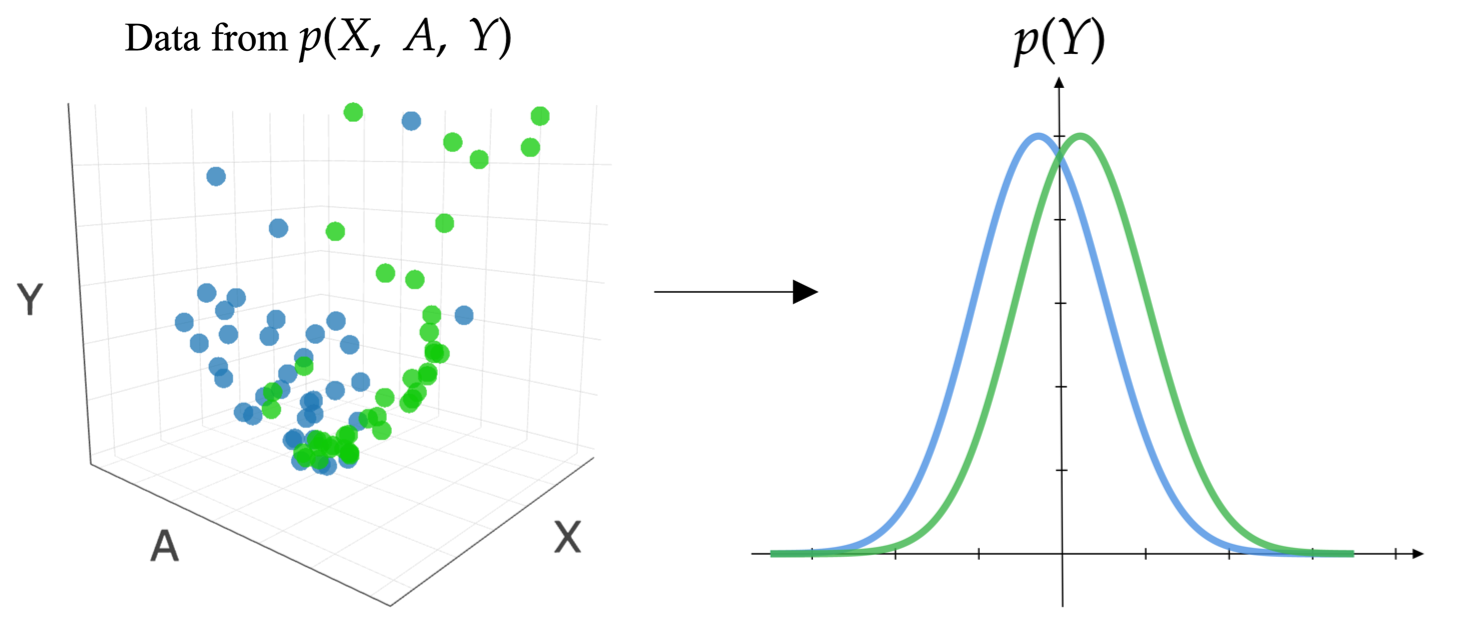
\includegraphics[width=0.5\textwidth]{figures/mr/main_pic.png}
%     \caption{Caption}
%     % \vspace{-1cm}
%     \label{fig:my_label}
% \end{wrapfigure}
In contextual bandits, the objective is to select an action $A$, guided by contextual information $X$, to maximize the resulting outcome $Y$. This paradigm is prevalent in many real-world applications such as healthcare, personalized recommendation systems, or online advertising \citep{li2010contextual, bastani2019online, xu2020contextual}. The objective is to perform actions, such as prescribing medication or recommending items, which lead to desired outcomes like improved patient health or higher click-through rates. Nonetheless, updating the policy presents challenges, as na\"ively implementing a new, untested policy may raise ethical or financial concerns. For instance, prescribing a drug based on a new policy poses risks, as it may result in unexpected side effects. As a result, recent research \citep{swaminathan2015counterfactual, wang2017optimal, farajtabar2018more, su2019continuous, metelli2021subgaussian, liu2019triply, sugiyama2012machine, swaminathan2017off} has concentrated on evaluating the performance of new policies (target policy) using only existing data that was generated using the current policy (behaviour policy). This problem is known as Off-Policy Evaluation (OPE).


Current OPE methods in contextual bandits, such as the Inverse Probability Weighting (IPW) \citep{horvitz1952generalization} and Doubly Robust (DR) \citep{dudik2014doubly} estimators primarily account for the policy shift by re-weighting the data using the ratio of the target and behaviour polices to estimate the target policy value. This can be problematic as it may lead to high variance in the estimators in cases of substantial policy shifts. The issue is further exacerbated in situations with large action or context spaces \citep{saito2022off}, since in these cases the estimation of policy ratios is even more difficult leading to extreme bias and variance.
% The problem is worsened in the policy ratios are even harder to estimate in these cases. 
% even when the distribution of outcome $Y$ changes minimally.
% \jef{Nonetheless, these methods possess a fundamental limitation, as they explicitly account for the shift between behavior and target policies when estimating the expected target policy value.} 
% As a result, the estimators may demonstrate high variance in cases of substantial policy shifts, even when the outcome distribution in $Y$ changes minimally. 
% This high variance in estimators can lead to unreliable and potentially vacuous outputs. 

% In light of these concerns, since our goal is to estimate the expected outcome $Y$ under a new target policy, we show that directly considering the shift in the marginal distribution of outcomes $Y$ rather than the shift in the policies leads to a more efficient estimator.

% Given our goal of estimating the expected outcome $Y$ under a new target policy, we show that directly considering the shift in the marginal distribution of outcomes $Y$

In this work we show that this problem of high variance in OPE can be alleviated by using methods which directly consider the shift in the marginal distribution of the outcome $Y$ resulting from the policy shift, instead of considering the policy shift itself (as in IPW and DR). To this end, we propose a new OPE estimator for contextual bandits called the Marginal Ratio (MR) estimator, which weights the data directly based on the shift in the marginal distribution of outcomes $Y$ and consequently is much more robust to increasing sizes of action and context spaces than existing methods like IPW or DR. 
% Since our goal is to estimate the expected outcome $Y$ under a new target policy, we show that 
% the problem of high variance that arises as a result of weighting the data using policy ratios can be circumvented by instead weighting the data directly based on the shift in the marginal distribution of outcomes $Y$.
% the problem of high variance can be alleviated by weighting the data directly based on the shift in the marginal distribution of outcomes $Y$ resulting from the policy shift rather than the policy ratios (as in IPW or DR).
% directly considering the shift in the marginal distribution of outcomes $Y$ rather than 
% To this end, we propose a new OPE estimator for contextual bandits called the Marginal Ratio (MR) estimator, which directly takes into account the shift in the marginal distribution of the outcome and consequently is much more robust to increasing sizes of action and context spaces than existing methods like IPW or DR. 
Our extensive theoretical analyses show that MR enjoys better variance properties than the existing methods making it highly attractive for a variety of applications in addition to OPE. One such application is the estimation of Average Treatment Effect (ATE) in causal inference, for which we show that MR provides greater sample efficiency than the most commonly used methods.

Our contributions in this paper are as follows:
% and can also be used in domains like causal inference for the estimation of Average Treatment Effect (ATE) where it leads to desirable properties such as increased sample efficiency 
% Additionally, we theoretically show that MR enjoys better variance properties than
% achieves significant variance reduction compared to 
% conventional methods (like IPW or DR) and consequently is much more robust to increasing sizes of action and context spaces.
% Additionally, we also show that the MR estimator can be applied in causal inference for the estimation of Average Treatment Effect (ATE). We demonstrate theoretically and empirically that the MR estimator is more sample efficient than existing methods. Our contributions in this paper are:



% by weighting the samples based on how relevant the observed \emph{outcome} is to the target outcome distribution.

% Our proposed method aims to offer a more robust solution, mitigating the adverse effects of high variance and providing a reliable alternative to existing OPE techniques. 
% At a high level, instead of weighting the samples based on the policy shift as in IPW, the MR estimator weights the samples based on how relevant the observed \emph{outcome} is to target outcome distribution.

% Current OPE methods in contextual bandits, such as the inverse propensity weighting (IPW) \citep{horvitz1952generalization} and doubly robust (DR) \citep{dudik2014doubly} estimators, have gained considerable popularity in practice due to their ability to estimate the expected value of a modified policy. However, these methods have an inherent limitation, as they explicitly consider the shift between behavior and target policies when estimating the target policy value. Consequently, the estimators can exhibit high variance when there is a significant policy shift, even if the change in the outcome distribution is minimal. This issue can be especially pronounced in scenarios with large action or context spaces \citep{saito2022off}.



% Contextual bandits are a prevalent framework \jef{need to rewrite this banditS are A framework doesnt sound right} used in several real-world applications, including healthcare, personalized recommendation systems, and online advertising \citep{li2010contextual, bastani2019online, xu2020contextual}\faaiz{more refs}. In this setup, an agent takes actions $A$ based on contextual information $X$, and receives outcomes $Y$ accordingly. In such settings \jef{Two times start with IN}, evaluating the effectiveness of a new policy without actually deploying it is often desirable \jef{Due to potential financial or ethical reasons + refs}. \jef{Would start this with: Hence, in recent years, researchers have ... }Off-policy evaluation (OPE) is a popular approach that estimates the expected value of a \jef{a or the?} random variable $Y$ under a target policy $\tar$, without deploying the target policy \citep{swaminathan2015counterfactual, wang2017optimal, farajtabar2018more, su2019continuous, metelli2021subgaussian, liu2019triply, sugiyama2012machine, swaminathan2017off}.

% Current OPE methods in contextual bandits focus on the shift in the joint distribution of the context, action, and outcome when estimating the expected value \jef{this sentence is coming out of nowhere}. These methods, such as the inverse propensity weighting (IPW) \citep{horvitz1952generalization} and doubly robust (DR) \citep{dudik2014doubly} estimators, have been highly popular in practice \jef{This should come first}. However, they have a fundamental limitation: they explicitly take the shift between behaviour and target policies into account when estimating target policy value. \jef{we might want to be more vague here in case people do not understand the problem of the ratios, or we have to be way more concrete}


% \jef{I will use AB review from now on :) }


% do not only take the shift in the distribution of the outcome into account, but also the shift in the distribution of the actions. 
% As a result, the estimators can have high variance when the policy shift is large, even if the shift in the outcome distribution is small. This issue can be particularly pronounced in large action or context spaces \citep{saito2022off}.

% To address this limitation, we propose a new OPE estimator for contextual bandits that only takes into account the shift in the marginal distribution of the outcome as a result of the policy shift. Our estimator, called Marginal Ratio (MR) estimator, utilizes the available logged data more efficiently and leads to lower variance than the current state-of-the-art methods. At a high level, instead of weighting the samples based on the policy shift as in IPW, the MR estimator weights the samples based on how relevant the observed \emph{outcome} is to target outcome distribution.
% assigns high weights to the samples where the observed outcomes are most relevant to the target outcome distribution.  

\begin{itemize}
    \item Firstly, we introduce MR, an OPE estimator for contextual bandits, that focuses on the shift in the marginal distribution of $Y$ rather than the joint distribution of $(X, A, Y)$. 
    \flag{We show that MR has favourable theoretical properties compared to existing methods like IPW and DR. Our analysis also encompasses theory on the approximation errors of our estimator. 
    % that MR achieves lower variance than conventional OPE methods like IPW.
    }
    % We provide extensive theoretical comparisons to show  the variance reduction properties of MR compared to existing approaches such as IPW and DR.
    % at MR achieves lower variance than IPW and DR estimators. 
    
    \item Secondly, we explicitly lay out the connection between MR and  Marginalized Inverse Propensity Score (MIPS) \cite{saito2022off}, a recent state-of-the-art contextual bandits OPE method, and prove that MR attains lowest variance among a generalized family of MIPS estimators. 
    \item Thirdly, we show that the MR estimator can be applied in the setting of causal inference to estimate average treatment effects (ATE), and theoretically prove that the resulting estimator is more data-efficient with higher accuracy and lower variance than commonly used methods. 
    \item Finally, we verify all our theoretical analyses through a variety of experiments on synthetic and real-world datasets and empirically demonstrate that the MR estimator achieves better overall performance compared to current state-of-the-art methods. 
\end{itemize}
% Firstly, we introduce MR, an OPE estimator for contextual bandits that focuses on the shift in the marginal distribution of $Y$ rather than the joint distribution of $(X, A, Y)$. Specifically, we provide extensive theoretical comparisons which show that MR achieves lower variance than classical importance-weighted estimators like IPW and DR. Our analysis also encompasses theory on the estimation errors of our estimator. Secondly, we explicitly layout the connection between MR and  Marginalized Inverse Propensity Score (MIPS) \cite{saito2022off}, a recent state-of-the-art contextual bandits OPE method, and demonstrate that MR attains lowest variance among a generalized family of MIPS estimators. Thirdly, we show that the MR estimator can be applied in the setting of causal inference to estimate average treatment effects (ATE), and theoretically prove that the resulting estimator is more data-efficient with higher accuracy and lower variance than commonly used methods. Finally, we verify all our theoretical analyses through a variety of experiments on synthetic and real-world datasets and empirically demonstrate that the MR estimator achieves better overall performance compared to current state-of-the-art methods. 

%  Our contributions in this paper are fourfold.
% \begin{enumerate}[label=\roman*.]
%     \item We introduce MR, an OPE estimator for contextual bandits that focuses on the shift in the marginal distribution of $Y$ rather than the joint distribution of $(X, A, Y)$. Specifically, we provide extensive theoretical comparisons 
%     which show that MR achieves lower variance than classical importance-weighted estimators like IPW and DR.
%     Our analysis also encompasses theory on the estimation errors of our estimator.
%     % In addition, we provide convergence rates for our estimator.
%     % Moreover, we show that MR is likely to achieve lower variance than the DR method when the dimensions of context $X$ are large.
%     % \item We provide theoretical results comparing the performance of MR against the most commonly used OPE estimators for contextual bandits. We prove that the variance of our estimator is lower than that of the classical importance-weighted estimator (IPW). Additionally, we contrast MR against the recently proposed MIPS estimator \citep{saito2022off} and show that MR achieves the optimal variance over the class of all MIPS estimators.
%     \item We explicitly layout the connection between MR and  Marginalized Inverse Propensity Score (MIPS) \cite{saito2022off}, a current state-of-the-art contextual bandits OPE method, and demonstrate that MR attains lowest variance among a generalized family of MIPS estimators.
%     \item We show that the MR estimator can be applied in the setting of causal inference to estimate average treatment effects (ATE), and theoretically prove that the resulting estimator is more data-efficient with higher accuracy and lower variance than commonly used methods.
%     \item We verify all our theoretical analyses through a variety of experiments on synthetic and real-world datasets and empirically demonstrate that the MR estimator achieves better overall performance compared to current state-of-the-art methods.
%     % \item We show that the MR estimator can be applied in the setting of causal inference to estimate average treatment effects (ATE), and leads to a more data-efficient estimator with higher accuracy and lower variance than the most commonly used methods.
%     % \item We verify our analysis on a variety of experiments on synthetic datasets as well as real-world datasets. We empirically show that MR achieves better performance overall compared to the current state-of-the-art methods.
% \end{enumerate}

% First, we propose a new off-policy evaluation (OPE) estimator, called MR, which only takes into account the shift in the marginal distribution of $Y$ instead of the joint distribution of $(X, A, Y)$. Second, we provide theoretical results comparing the performance of MR against the most commonly used OPE estimators for contextual bandits. We prove that the variance of our estimator is lower than that of the classical importance-weighted estimator (IPW). Additionally, we contrast MR against the recently proposed MIPS estimator \citep{saito2022off} and show that MR achieves the optimal variance over the class of all MIPS estimators. Third, we show that the MR estimator can be applied in the setting of causal inference to estimate average treatment effects (ATE), and leads to a more data-efficient estimator with high accuracy and low variance than the most commonly used methods.  Finally, we verify our analysis on a variety of experiments on synthetic datasets as well as real-world datasets. We empirically show that MR achieves better performance overall compared to the current state-of-the-art methods. 
% Our proposed method, MR, can therefore be seen as a significant contribution to the field of off-policy evaluation for contextual bandits.

% Specifically, we provide theoretical results showing that the variance of MR is lower than those of the classical IPW estimator, and the recently proposed MIPS estimator \citep{saito2022off}. We also show that MR achieves the optimal variance over the class of all MIPS estimators.

% In addition to the theoretical analysis, we evaluate the performance of MR on both synthetic and real-world classification datasets. Our experiments demonstrate that MR achieves better performance overall compared to the existing methods. Overall, our proposed MR estimator presents a significant contribution to the OPE problem in contextual bandits, providing a more efficient and accurate way to estimate the expected value of a random variable under a target policy


\section{Background}
\subsection{Setup and Notation} \label{sec:setup_notation}
We consider the standard contextual bandit setting. Let $X\in\Xspace$ be a context vector (e.g., user features), $A\in \Aspace$ denote an action (e.g., recommended website to the user), and $Y\in \Yspace$ denote a scalar reward or outcome (e.g., whether the user clicks on the website). The outcome and context are sampled from unknown probability distributions $p(y\mid x, a)$ and $p(x)$ respectively. Let $\D\coloneqq \{(x_i, a_i, y_i)\}_{i=1}^n$ be a historically logged dataset with $n$ observations, generated by a (possibly unknown) \emph{behaviour policy} $\beh(a\mid x)$.
Specifically, $\D$ consists of i.i.d. samples from the joint density under\textit{ behaviour policy},
\begin{align}
    \pbeh(x, a, y) \coloneqq p(y\mid x, a)\, \textcolor{blue}{\beh(a\mid x)}\,p(x). \label{eq:behav-joint-factorisation}
\end{align}
We denote the joint density of $(X, A, Y)$ under the \textit{target policy} as
\begin{align}
    \ptar(x, a, y) \coloneqq p(y\mid x, a)\, \textcolor{red}{\tar(a\mid x)}\,p(x). \label{eq:tar-joint-factorisation}
\end{align}

Moreover, we use $\pbeh(y)$ to denote the marginal density of $Y$ under the behaviour policy, 
\begin{align*}
    \pbeh(y) &= \int_{\Aspace \times \Xspace} \pbeh(x, a, y)\, \mathrm{d}a \, \mathrm{d}x,
\end{align*}
and likewise for the target policy $\tar$. Similarly, we use $\Ebeh$ and $\Etar$ to denote the expectations under the joint densities $\pbeh(x, a, y)$ and $\ptar(x, a, y)$ respectively.


\myparagraph{Off-policy evaluation (OPE)}
The main objective of OPE is to estimate the expectation of the outcome $Y$ under a given target policy $\tar$, i.e., $\Etar [Y]$, using only the logged data $\D$.
% \[
% \Etar [Y] \coloneqq \E_{(X, A, Y) \sim \ptar}[Y].
% \]


% \paragraph{Notation}
% We use $\pbeh(x, a, y)$ to denote the joint density of $(X, A, Y)$ under the behaviour policy, and $\ptar(x, a, y)$ to denote the joint density under target policy. The joint densities, whose factorisation only differs in the policies, can be written as follows:
% \begin{align}\label{eq:pxay}
%     \pbeh(x, a, y) &= p(y\mid x, a)\, \textcolor{blue}{\beh(a\mid x)}\,p(x), \\
%     \ptar(x, a, y) &= p(y\mid x, a)\, \textcolor{red}{\tar(a\mid x)}\,p(x).
% \end{align}
% The historical logged data $\D$ comprises i.i.d. realisations from the joint density $\pbeh(x, a, y)$.
% Moreover, we use $\pbeh(y)$ to denote the marginal density of $Y$ under the behaviour policy, 
% \begin{align*}
%     \pbeh(y) &= \int_{\Aspace, \Xspace} \pbeh(x, a, y)\, \mathrm{d}a \, \mathrm{d}x,
% \end{align*}
% and likewise for the target policy $\tar$. Similarly, we use $\Ebeh$ and $\Etar$ to denote the expectations under the joint densities $\pbeh(x, a, y)$ and $\ptar(x, a, y)$ respectively.

% \paragraph{Off-policy evaluation}
% Given logged data $\D$, our goal is to estimate the following expectation
% \[
% \Etar [Y] \coloneqq \E_{(X, A, Y) \sim \ptar}[Y].
% \]

Throughout this work, we assume that the support of the target policy $\tar$ is included in the support of the behaviour policy $\beh$. This is to ensure that importance sampling yields unbiased off-policy estimators, and is satisfied for exploratory behaviour policies such as the $\epsilon$-greedy policies. 
\begin{assumption}[Support]
    For any $x \in \Xspace, a \in \Aspace$,  $\tar(a\mid x) >0 \implies \beh(a\mid x) >0$. 
\end{assumption}
% This is a mild assumption which
 

\subsection{Existing off-policy evaluation methodologies}
Next, we will present some of the most commonly used OPE estimators before outlining the limitations of these methodologies. This motivates our proposal of an alternative OPE estimator. 

The value of the target policy can be expressed as the expectation of outcome $Y$ under the target data distribution $\ptar(x, a, y)$.
% The policy value of target policy $\tar$ can be written as:
% \[
% \Etar[Y] = \int_{\Xspace, \Aspace, \Yspace} y\, \ptar(x, a, y) \, \mathrm{d}x \, \mathrm{d}a \, \mathrm{d}y.
% \]
However in most cases, we do not have access to samples from this target distribution and hence we have to resort to importance sampling methods.
\paragraph{Inverse Probability Weighting (IPW) estimator}
One way to compute the target policy value, $\Etar[Y]$, when only given data generated from $\pbeh(x, a, y)$ is to rewrite the policy value as follows:
% _{\Xspace, \Aspace, \Yspace}
\begin{small}
\begin{align*}
    \Etarred[Y] =
    \int y \, \ptar(x, a, y) \,\mathrm{d}y \, \mathrm{d}a\, \mathrm{d}x   =
    \int y \, \underbrace{\frac{\ptar(x, a, y)}{\pbeh(x, a, y)}}_{\rho(a,x)}\, \pbeh(x, a, y) \,\mathrm{d}y \, \mathrm{d}a\, \mathrm{d}x =
    % \Ebehblue\left[Y\,\frac{\ptar(X, A, Y)}{\pbeh(X, A, Y)} \right] = 
    \Ebehblue\left[Y\,\rho(A, X)\right],
\end{align*}
\end{small} 
where 
$
\rho(a, x) \coloneqq \frac{\ptar(x, a, y)}{\pbeh(x, a, y)} = \frac{\tar(a|x)}{\beh(a|x)}
$, given the factorizations in Eqns. \eqref{eq:behav-joint-factorisation} and \eqref{eq:tar-joint-factorisation}.
This leads to the commonly used \emph{Inverse Probability Weighting (IPW)} \citep{horvitz1952generalization} estimator:
\[
\thetaipw \coloneqq \frac{1}{n}\sum_{i=1}^n \rho(a_i, x_i)\,y_i.
\]
When the behaviour policy is known, IPW is an unbiased and consistent estimator. However, it can suffer from high variance, especially as the overlap between the behaviour and target policies decreases. 

\myparagraph{Doubly Robust (DR) estimator} 
To alleviate the high variance of IPW, \cite{dudik2014doubly} proposed a \emph{Doubly Robust (DR)} estimator for OPE. 
DR uses an estimate of the conditional mean $\hat{\mu}(a, x) \approx\E[Y\mid X=x, A=a]$ (\emph{outcome model}), as a control variate to decrease the variance of IPW. It is also doubly robust in that it yields accurate value estimates if either the importance weights $\rho(a, x)$ or the outcome model $\hat{\mu}(a, x)$ is well estimated \citep{dudik2014doubly, jiang2016doubly}. 
The DR estimator for $\Etar[Y]$ can be written as follows:
\[
\thetadr = \frac{1}{n} \sum_{i=1}^n \rho(a_i, x_i)\,(y_i - \hat{\mu}(a_i, x_i)) + \hat{\eta}(\tar),
% \vspace{-0.7mm}
\]
where
$
\hat{\eta}(\tar) = \frac{1}{n} \sum_{i=1}^n \sum_{a'\in \Aspace} \hat{\mu}(a', x_i) \tar(a'\mid x_i) \approx \E_{\tar}[\hat{\mu}(A, X)]$. Here, $\hat{\eta}(\tar)$ is referred to as the Direct Method (DM) as it uses $\hat{\mu}(a, x)$ directly to estimate target policy value. 

\subsection{Limitation of existing methodologies} 
To estimate the value of the target policy $\tar$, the existing methodologies consider the shift in the joint distribution of $(X, A, Y)$  as a result of the policy shift (by weighting samples by policy ratios). As we show in Section \ref{subsec:comparison}, considering the joint shift can lead to inefficient policy evaluation and high variance especially as the policy shift increases \citep{li2018addressing}.
Since our goal is to estimate $\Etar[Y]$, we will show in the next section that considering only the shift in the marginal distribution of the outcomes $Y$ from $\pbeh(Y)$ to $\ptar(Y)$, leads to a more efficient OPE methodology compared to existing approaches.

To better comprehend why only considering the shift in the marginal distribution is advantageous, let us examine an extreme example where we assume that $Y \indep A \mid X$, i.e., the outcome $Y$ for a user $X$ is independent of the action $A$ taken. In this specific instance, $\Etar[Y] = \Ebeh[Y] \approx 1/n\sum_{i=1}^n y_i,$ indicating that an unweighted empirical mean serves as a suitable unbiased estimator of $\Etar[Y]$. However, IPW and DR estimators use policy ratios $\rho(a, x)  = \frac{\tar(a \mid x)}{\beh(a \mid x)}$ as importance weights. In case of large policy shifts, these ratios may vary significantly, leading to high variance in IPW and DR.

In this particular example, the shift in policies is inconsequential as it does not impact the distribution of outcomes $Y$. Hence, IPW and DR estimators introduce additional variance due to the policy ratios when they are not actually required. This limitation is not exclusive to this special case; in general, methodologies like IPW and DR exhibit high variance when there is low overlap between target and behavior policies \citep{li2018addressing} even if the resulting shift in marginals of the outcome $Y$ is not significant.
% This limitation is not exclusive to this special case; in general, methodologies like IPW and DR that use policy ratios as importance weights exhibit high variance when there is low overlap between target and behavior policies \citep{li2018addressing} or when the action and/or context spaces are large \citep{saito2022off}.

Therefore, we propose the \emph{Marginal Ratio (MR)} OPE estimator for contextual bandits in the subsequent section, which circumvents these issues by focusing on the shift in the marginal distribution of the outcomes $Y$. Additionally, we provide extensive theoretical insights on the comparison of MR to existing state-of-the-art methods, such as IPW and DR.

% To estimate the value of the target policy $\tar$, the existing methodologies consider the shift in the joint distribution of $(X, A, Y)$ as a result of the policy shift. As we show in Section \ref{subsec:comparison}, considering the joint shift can lead to inefficient policy evaluation and high variance especially as the policy shift increases \citep{li2018addressing}.
% Since our goal is to estimate $\Etar[Y]$, we will show in the next section that considering only the shift in the marginal distribution of the outcomes $Y$ from $\pbeh(Y)$ to $\ptar(Y)$, leads to a more efficient OPE methodology compared to existing approaches.

% To gain a better intuitive understanding why only considering the shift in the marginal distribution, let us take this extreme example, where we assume that $Y \indep A \mid X$, i.e. the outcome $Y$ of a user $X$ does not depend on the action taken. In this special example, $\Etar[Y] = \Ebeh[Y] \approx 1/n\sum_{i=1}^n y_i,$ and therefore, an unweighted empirical mean should be a good unbiased estimator of $\Etar[Y]$. However, the IPW and DR estimators use the policy ratios as importance weights since $\ptar(x, a, y)/\pbeh(x, a, y) = \tar(a \mid x)/\beh(a \mid x)$, and hence yield a higher variance estimator. 

% In this specific example, the shift in policies is meaningless as it has no effect on the distribution of outcomes $Y$, and therefore, the IPW and DR estimators incur extra variance due to the importance ratios when they are in fact not needed. This limitation is not restricted to this special case and in general, methodologies like IPW and DR which use policy ratios as importance weights will have high variance whenever there is low overlap between target and behaviour policies \citep{li2018addressing} or whenever the action and/or context spaces are large \citep{saito2022off}.

% Hence, we propose \emph{Marginal Ratio (MR)} OPE estimator for contextual bandits in the next section, which avoids these problems by only considering the shift in the marginal distribution of the outcomes $Y$. In addition, using the MR estimator, we are able to gain novel theoretical insights compared to existing SOTA methods such as IPW and DR methods in terms of variance reduction.






% Since our goal is to estimate $\Etar[Y]$, it suffices to consider only the shift in the marginal distribution of the outcomes $Y$ from $\pbeh(y)$ to $\ptar(y)$. Instead, methodologies like IPW and DR consider the shift in the joint distribution of $(X, A, Y)$ which can lead to inefficient policy evaluation and high variance especially as the policy shift increases \citep{li2018addressing}.
% In the next section, we propose \emph{Marginal Ratio (MR)} OPE estimator which circumvents the limitations outlined above, by only considering the shift in the marginal distribution of the outcomes $Y$. 
% Similarly, we could also consider another example, where the action $a \in [-100, 100]$ is related to $Y$ through a simple function such as $Y=x$ for $a < 0$ and $Y=-x$ for $a > 0$. In this case, modelling the ratio of the policy which for ever action, would unnecessarily complicate as computation. \jef{to be completed}
% \jef{TODO} The following special case makes this idea more concrete. Assume that $Y \indep A \mid X$, i.e. the outcome $Y$ of a user $X$ does not depend on the action taken. In this case $\Etar[Y] = \Ebeh[Y] \approx 1/n\sum_{i=1}^n y_i,$ and therefore, an unweighted empirical mean should be a good unbiased estimator of $\Etar[Y]$. However, the IPW and DR estimators use the policy ratios as importance weights since $\ptar(x, a, y)/\pbeh(x, a, y) = \tar(a \mid x)/\beh(a \mid x)$, and hence yield a weighted estimator. \faaiz{to be fixed}

\section{Marginal Ratio (MR) estimator}
 
% \subsection{Marginal Ratio (MR) estimator}
% The main insight of our methodology is to weight the outcomes using the ratio of marginal density of the outcome $Y$, i.e.,
Our method's key insight involves weighting outcomes by the marginal density ratio of outcome $Y$:
\begin{align*}
\Etarred[Y] &= \int_{\Yspace} y \, \ptar(y)\, \mathrm{d}y = \int_\Yspace y\, \frac{\ptar(y)}{\pbeh(y)} \, \pbeh(y) \, \mathrm{d}y = \Ebehblue\left[Y\, w(Y) \right],
\end{align*}
where 
$
w(y) \coloneqq \frac{\ptar(y)}{\pbeh(y)}.
$
This leads to the Marginal Ratio OPE estimator:
\begin{align*}
    \thetamr \coloneqq \frac{1}{n}\sum_{i=1}^n w(y_i) \, y_i.
\end{align*}

In Section \ref{subsec:comparison} we prove that by only considering the shift in the marginal distribution of outcomes, the MR estimator achieves a lower variance than the standard OPE methods. In fact, this estimator does not depend on the shift between target and behaviour policies directly. Instead, it depends on the shift between the marginals $\pbeh(y)$ and $\ptar(y)$.
% Moreover, when the weights $w(y)$ are known exactly, the MR estimator is unbiased and consistent.
% \jef{I recon we can chuck this}
% \jef{Need to change and think as well} Recall that in our previous example with $Y \indep A\mid X$, any policy shift has no effect on the marginal outcome distribution and the weights $w(y)\equiv 1$ for any target and behaviour policies. Therefore $\thetamr = 1/n \sum_{i=1}^n y_i$, i.e., MR leads to an unweighted estimator which is unbiased and does not incur any extra variance arising from the importance weights $\tar(a\mid x)/\beh(a\mid x)$.
% Before we go on to prove the variance reduction, we first outline how to efficiently compute the weights $w(y)$ using the logged data $\D$.
% To start, let us outline an efficient way to estimate the weights $w(y)$ using the logged data $\D$, before moving on to prove the variance reduction.

\myparagraph{Estimation of $w(y)$} When the weights $w(y)$ are known exactly, the MR estimator is unbiased and consistent. However, in practice the weights $w(y)$ are often not known and must be estimated using the logged data $\D$. Here, we outline an efficient way to estimate $w(y)$ by first representing it as a conditional expectation, which can subsequently be expressed as the solution to a regression problem.
% \jef{Add references as mentioned by Arnaud}
% \begin{align}\label{eq:ratioidentity}
%     w(y)=\frac{\ptar(y)}{\pbeh(y)} =\int_{\Xspace, \Aspace} \frac{\ptar(x,a,y)}{\pbeh(x,a,y)}\,\pbeh(a, x|y)\,\mathrm{d}a\, \mathrm{d}x  
%     % &=\int_{\Xspace, \Aspace} \frac{\pi^{\ast}(a|x)}{\beh (a|x)}\,\pbeh(a, x|y)\,\mathrm{d}a \,\mathrm{d}x \nonumber\\
%     &= \Ebeh\Bigg[ \frac{\pi^{\ast}(A|X)}{\beh (A|X)} \Bigg| \,Y=y \Bigg]. 
% \end{align}
% \faaiz{make this a complete sentence}
\begin{lemma}\label{lemma:weights-est}
Let $w(y)=\frac{\ptar(y)}{\pbeh(y)}$ and $\rho(a, x) = \frac{\tar(a\mid x)}{\beh(a\mid x)}$, then $w(y) = \Ebeh\left[ \rho(A, X) \mid \,Y=y \right]$, and,
% \[
% w(y)= \Ebeh\left[ \rho(A, X) \mid \,Y=y \right], \quad \textup{and consequently,} \quad w = \arg\min_{f} \, \Ebeh \left[(\rho(A, X)-f(Y))^2\right]. 
% \]
% Additionally,
\begin{align}
 w = \arg\min_{f} \, \Ebeh \left[(\rho(A, X)-f(Y))^2\right]. \label{eq:weights-obj}
\end{align}
\end{lemma}
% \vspace{-2mm}
Lemma \ref{lemma:weights-est} allows us to approximate $w(y)$ using a parametric family $\{f_\phi: \mathbb{R}\rightarrow \mathbb{R} \mid \phi \in \Phi\}$ (e.g.\ neural networks) and defining $\hat{w}(y)\coloneqq f_{\phi^*}(y)$, where $\phi^*$ solves the regression problem in Eq. \eqref{eq:weights-obj}. 

% Hence, the weights $w(y)$ can be estimated by solving the regression problem in Eq. \eqref{eq:weights-obj}. 
% Similar techniques of estimating ratios of marginal densities have also been used in areas like likelihood-free inference \citep{brehmer2020mining}.
% Similar techniques have also been used in areas like likelihood-free inference \citep{brehmer2020mining} to estimate the ratio of marginal densities.

% \paragraph{Proof of Lemma \ref{prop:weights-est}}
% This follows directly from the identity \eqref{eq:ratioidentity}. 
% We prove it here for the sake of completeness.
% \begin{align}
%     &\Ebeh \Bigg[\frac{\pi^{\ast}(A|X)}{\beh (A|X)}-f(Y)\Bigg]^2 \nonumber \\
%     &= \mathbb{E}_{X,Y \sim P^{\beh}_{X,Y}} \Big[\E_{A \sim P^{\beh}_{A\mid X,Y}} \Big|\Big|\frac{\pi^{\ast}(A|X)}{\beh (A|X)}-f(X,Y)\Big|\Big|^2\Big] \nonumber \\
%     &= \mathbb{E}_{X,Y \sim P^{\beh}_{X,Y}} \Big[\textup{Var}_{A \sim P^{\beh}_{A\mid X,Y}}\Big[ \frac{\pi^{\ast}(A|X)}{\beh (A|X)} \Big] + \left(\E_{A \sim P^{\beh}_{A\mid X,Y}}\Big[ \frac{\pi^{\ast}(A|X)}{\beh (A|X)} \Big] - f(X,Y) \right)^2 \Big].
%      \label{eq:w-reg}
% \end{align}
% Where, \eqref{eq:w-reg} is minimized if $f(x, y) = \E_{A \sim P^{\beh}_{A\mid X=x,Y=y}}\Big[ \frac{\pi^{\ast}(A|x)}{\beh (A|x)} \Big] = w(x,y)$.

% \begin{align}
%     \theta^* \coloneqq \arg \min_{\theta} \Ebeh \Bigg(\frac{\pi^{\ast}(A|X)}{\beh (A|X)}-f_\theta(Y)\Bigg)^2 \label{eq:weights-loss}
% \end{align}

Note that MR can also be estimated alternatively by directly estimating $h(y) \coloneqq w(y)\,y$ 
% (instead of estimating the weights $w(y)$) 
using a similar regression technique as above and computing $\thetamr = 1/n \sum_{i=1}^n h(y_i)$. We include additional details along with empirical comparisons in Appendix \ref{sec:alt-estimation-method}. 
% In the next section, we provide theoretical analysis comparing the MR estimator with the existing methodologies. 

\begin{comment}
\subsubsection{Alternative estimation method}\label{sec:alt-estimation-method}
When estimating the MR estimator, we can alternatively estimate $h(y) \coloneqq y\,w(y)$ using 
\begin{align*}
    h = \arg\min_{f} \, \Ebeh \Bigg(Y\,\frac{\tar(A|X)}{\beh (A|X)}-f(Y)\Bigg)^2.
\end{align*}
Subsequently, the MR estimator can be written as:
\[
\thetamr = \frac{1}{n}\sum_{i=1}^n h(y_i).
\]
\paragraph{Remark}
These methods outline two different methodologies of estimating MR. In general, it is difficult to say which of the two methods will perform better. Intuitively speaking, in cases where the behaviour of the quantity $Y\,\frac{\tar(A|X)}{\beh (A|X)}$ with varying $Y$ is `smoother' than that of $\frac{\tar(A|X)}{\beh (A|X)}$, the alternative method is expected to perform better. Our empirical results in Appendix \ref{app:experiments} shows that the relative performance of the two methods varies for different data generating mechanisms.

% \faaiz{talk about the comparison between the two methods}

\rob{We could alternatively write $\Etar[Y] = \Ebeh[\Ebeh[Y \, \frac{\pi^\ast(A|X)}{\beh(A|X)} \mid Y]]$, regress $h_\theta(y) \approx \Ebeh[Y \, \frac{\pi^\ast(A|X)}{\beh(A|X)} \mid Y = y]$, and approximate $\Etar[Y] \approx \frac{1}{n} \sum_{i=1}^n h_\theta(Y_i)$. Is there a reason not to prefer this approach?}

\arnaud{indeed Rob, actually i conjecture that this should be better - think of a case where the policy ratio is high in regions where the outcome is null - with Rob's approach you won't need to bother approximating the ratio of marginal returns in those regions... i think that then the theoretical result will be less elegant -- in any case, this should be tried and mentioned in the paper}
\end{comment}

\subsection{Theoretical analysis}\label{subsec:comparison}
Recall that the traditional OPE estimators like IPW and DR use importance weights which account for the the shift in the joint distributions of $(X, A, Y)$. In this section, we prove that by considering only the shift in the marginal distribution of $Y$ instead, MR achieves better variance properties than these estimators.
% , which considers the shift in the marginal distribution of $Y$, achieves lower variance than the existing methods. 
Our analysis in this subsection assumes that the ratios $\rho(a, x)$ and $w(y)$ are known exactly. Since the OPE estimators considered are unbiased in this case, 
our analysis of variance is analogous to that of the mean squared error (MSE) here.
% Since the OPE estimators considered are unbiased in this case, we only need to compare the variance of these estimators. 
We address the case where the weights are not known exactly in Section \ref{subsec:weight-estimation-error}.
First, we make precise our intuition that the shift in the joint distribution of $(X, A, Y)$ is `greater' than the shift in the marginal distribution of outcomes $Y$. 
We formalise this using the notion of $f$-divergences.
\begin{proposition}\label{tv_prop}
Let $f:[0, \infty) \rightarrow \mathbb{R}$ be a convex function with $f(1)=0$, and $\textup{D}_f(P || Q)$ denotes the $f$-divergence between distributions $P$ and $Q$. Then,
\[
\textup{D}_f\left(\ptar(x,a,y)\,||\, \pbeh(x,a,y)\right) \geq \textup{D}_f\left(\ptar(y)\,||\, \pbeh(y)\right).
\]
\end{proposition}

\begin{comment}
\begin{proposition}\label{tv_prop}
Let $\textup{TV}(P, Q)$ denote the total variation distance between densities $P$ and $Q$. Then,
$$
\textup{TV}\left(\pbeh(x, a, y), \ptar(x, a, y)\right) \geq \textup{TV}\left(\pbeh(y), \ptar(y)\right).
$$
\end{proposition}
\begin{proof}
\begin{align}
    \textup{TV}\left(\pbeh(x, a, y), \ptar(x, a, y)\right) &= 1/2 \int_{\Xspace, \Aspace,\Yspace} |\pbeh(x, a, y) - \ptar(x, a, y) | \, \mathrm{d}x \,\mathrm{d}a \, \mathrm{d}y \nonumber\\
    &\geq 1/2 \int_\Yspace\left| \int_{\Xspace,\Aspace} \pbeh(x, a, y) - \ptar(x, a, y) \, \mathrm{d}a \, \mathrm{d}x \right| \mathrm{d}y \nonumber\\
    &= 1/2 \int_\Yspace |\pbeh(y) - \ptar(y)|\, \mathrm{d}y \nonumber\\
    &= \textup{TV}\left(\pbeh(y), \ptar(y)\right) \nonumber
\end{align}
\end{proof}
\end{comment}
\paragraph{Intuition}
Proposition \ref{tv_prop} shows that the shift in the joint distributions is at least as `large' as the shift in the marginals of the outcome $Y$. Traditional OPE estimators, therefore take into consideration more of a distribution shift than needed, and consequently lead to inefficient estimators. In contrast, the MR estimator mitigates this problem by only considering the shift in the marginal distributions of outcomes resulting from the policy shift. 
% This intuition is made precise in \faaiz{ref}, which shows that the number of datapoints needed for accurate importance sampling estimates is directly related to the KL-divergence between two distributions
This provides further intuition on why the MR estimator has lower variance compared to existing methods. 
% Moreover, this result can also be used to prove that th
% \flag{This intuition is also supported by \cite{chatterjee2018sample}.}
% , which shows that the accuracy of an importance sampling mean estimate is directly related to the KL-divergence (which is an $f$-divergence) between the data distribution and the target distribution.
% For instance, in our example with $Y \indep A\mid X$, the weights $w(y)\equiv 1$ for any target and behaviour policies as any policy shift has no effect on the marginal outcome distribution, and therefore $\thetamr = 1/n \sum_{i=1}^n y_i$. 

% \jef{possible remove}
% Additionally, we emphasise the generality of Proposition \ref{tv_prop}, as it holds for the large class of $f$-divergences which includes the most commonly used divergences such as KL-divergence, total variation distance and $\chi^2$-divergences. In particular, by using $f(x) = (x-1)^2$ in Proposition \ref{tv_prop} we obtain that the variance of marginal density ratios $w(Y)$ is smaller than that of the policy ratio $\rho(A, X)$. This provides further intuition on why the MR estimator has lower variance compared to existing methods.
% This also results in the MR estimator having a lower variance than the IPW estimator. 

\begin{comment}
    
In fact, as we show next, Proposition \ref{tv_prop} implies that on average the marginal density ratio is closer to 1 than the joint density ratio (i.e., the policy ratio), and moreover, the variance of marginal density ratio is also smaller than that of the policy ratio. 
% using $f(x) = |x - 1|$ it follows straightforwardly from Proposition \ref{tv_prop} that on average the marginal density ratio is closer to 1 than the joint density ratio (i.e., the policy ratio). We formalise this in the following corollary.
\begin{corollary}
\begin{align*}
    f(x) = |x-1| \quad\textup{in Proposition \ref{tv_prop}} &\implies \Ebeh\left|\rho(A, X) - 1 \right| \geq \Ebeh\left|w(Y) - 1 \right|,\\
    f(x) = (x-1)^2 \quad\textup{in Proposition \ref{tv_prop}} &\implies \Vbeh(\rho(A, X)) \geq \Vbeh(w(Y)),
\end{align*}
where $\rho(a, x) \coloneqq \frac{\ptar(x, a, y)}{\pbeh(x, a, y)} =\frac{\tar(a|x)}{\beh(a|x)}$.
% Using $f(x) = |x-1|$ in Proposition \ref{tv_prop}: $\Ebeh\left|\rho(A, X) - 1 \right| \geq \Ebeh\left|w(Y) - 1 \right|$.\\
% Using $f(x) = (x-1)^2$ in Proposition \ref{tv_prop}: $\Vbeh(\rho(A, X)) \geq \Vbeh(w(Y))$.
% % \begin{align}
% %     \Ebeh\left|\rho(A, X) - 1 \right| \geq \Ebeh\left|w(Y) - 1 \right|
% % \end{align}
\end{corollary}
\paragraph{Intuition} As a consequence of only considering the marginal shift, the weights $w(Y)$ are `closer' to 1 on average than the ratio of joint distributions $\rho(A, X)$, and the variance of $w(Y)$ is smaller than that of $\rho(A, X)$. This also results in the MR estimator having a lower variance than the IPW estimator.
% \faaiz{we can also similarly prove that variance of $\rho(A, X)$ is greater than that of $w(Y)$ using $f(x) = (x-1)^2$.}
\end{comment}

\begin{proposition}[Variance comparison with IPW estimator]\label{prop:var_mr}
When the weights $\rho(a, x)$ and $w(y)$ are known exactly, we have that $\Vbeh[\thetamr] \leq \Vbeh[\thetaipw]$. In particular,
\begin{align*}
    \Vbeh[\thetaipw] - \Vbeh[\thetamr]
    = \frac{1}{n} \Ebeh \left[ \Vbeh\left[ \rho(A, X) \mid Y \right]\, Y^2 \right] \geq 0.
\end{align*}
\end{proposition}
\myparagraph{Intuition}
Proposition \ref{prop:var_mr} shows that the variance of MR estimator is smaller than that of the IPW estimator when the weights are known exactly. 
% Since MR is unbiased in this case, our analysis in this section mainly focuses on the variance. We also address the case where the weights are not known exactly in Section \ref{subsec:weight-estimation-error} by analysing the resulting bias and variance of MR. 
Moreover, the proposition also shows that the difference between the two variances will increases as the variance $\Vbeh\left[ \rho(A, X) \mid Y \right]$ increases. This variance is likely to be large when the policy shift between $\beh$ and $\tar$ is large, or when the dimensions of contexts $X$ and/or the actions $A$ is large, and therefore in these cases the MR estimator will perform increasingly better than the IPW estimator.
% The proposition therefore suggests that the MR estimator performs increasingly better than the IPW estimator as the difference between target and behaviour policy increases or the dimension of $\Xspace$ and/or $\Aspace$ increases. 
A similar phenomenon occurs for DR as we show next, even though in this case the variance of MR is not in general smaller than that of DR. 

\begin{proposition}[Variance comparison with DR estimator]\label{prop:var_dr}
When the weights $\rho(a, x)$ and $w(y)$ are known exactly and $\mu(A, X) \coloneqq \E[Y\mid X, A]$, we have that,
\begin{align*}
     \Vbeh[\thetadr] - \Vbeh[\thetamr]
    \geq \frac{1}{n} \Ebeh \left[ \Vbeh\left[\rho(A, X)\,Y \mid Y \right] -  \Vbeh\left[\rho(A, X)\,\mu(A, X) \mid X \right] \right].
\end{align*}
\end{proposition}
\paragraph{Intuition}
Proposition \ref{prop:var_dr} shows that if $\Vbeh\left[ \rho(A, X)\,Y \mid Y \right]$ is greater than $\Vbeh\left[ \rho(A, X)\,\mu(A, X) \mid X \right]$ on average, the variance of the MR estimator will be less than that of the DR estimator. 
% In other words, 
% the MR estimator will achieve lower variance 
% will not always have lower variance than DR, however, 
Intuitively, this will occur when the dimension of context space $\Xspace$ is high because in this case the conditional variance over $X$ and $A$, $\Vbeh\left[\rho(A, X)\,Y \mid Y \right]$ is likely to be greater than the conditional variance over $A$, $\Vbeh\left[ \rho(A, X)\,\mu(A, X) \mid X \right]$. Our empirical results in Appendix \ref{subsec:mips-empirical} are consistent with this intuition.
Additionally, we also provide theoretical comparisons with other extensions of DR, such as Switch-DR \citep{wang2017optimal} and DR with Optimistic Shrinkage (DRos) \citep{su2020doubly} in Appendix \ref{sec:dr-extensions}, and show that a similar intuition applies for these results. 
\flag{We emphasise that the well known results in \cite{wang2017optimal} which show that IPW and DR estimators achieve the optimal \emph{worst case} variance (where the worst case is taken over a class of possible outcome distributions $Y\mid X, A$) are not at odds with our results presented here (as the distribution of $Y\mid X, A$ is fixed in our setting).}
% We can also show that in the special case when $Y \indep (A, X)$, we have that $\Vbeh[\thetadr] \geq \Vbeh[\thetamr]$ \faaiz{show this}. 
% This may not be the case in practice and in Section \faaiz{ref} we consider the case where the weights are not known.

\subsubsection{Comparison with Marginalised Inverse Propensity Score (MIPS) \citep{saito2022off}}\label{subsec:mips-comparison}
In this section, we compare MR against the recently proposed Marginalised Inverse Propensity Score (MIPS) estimator \citep{saito2022off}, which uses a marginalisation technique to reduce variance and provides a robust OPE estimate specifically in contextual bandits with large action spaces. We prove that the MR estimator achieves lower variance than the MIPS estimator and doesn't require new assumptions.
% If the goal is to obtain OPE estimators with low variance, various analogues of the MR estimator can be considered which use marginalisation techniques to reduce the variance of the resulting estimators. The recently proposed Marginalised Inverse Propensity Score (MIPS) estimator \citep{saito2022off} is one such method which uses a marginalisation technique to reduce variance and provide robust OPE estimates specifically in contextual bandits with large action spaces. 


% We prove that the MR estimator achieves a lower variance than the MIPS estimator and unlike the MIPS estimator, does not require introducing any new assumptions. 

\myparagraph{MIPS estimator}
As we mentioned earlier, the variance of the IPW estimator may be high when the action $A$ is high dimensional. To mitigate this, the MIPS estimator assumes the existence of a (potentially lower dimensional) action embedding $E$, which summarises all `relevant' information about the action $A$. Formally, this assumption can be written as follows: 
\begin{assumption}\label{assum:indep-mips}
    The action $A$ has no direct effect on the outcome $Y$, i.e., 
    $$Y \indep A \mid X, E.$$
\end{assumption}
For example, in the setting of a recommendation system where $A$ corresponds to the items recommended, $E$ may correspond to the item categories. Assumption \ref{assum:indep-mips} then intuitively means that item category $E$ encodes all relevant information about the item $A$ which determines the outcome $Y$. Assuming that such action embedding $E$ exists, \cite{saito2022off} prove that the MIPS estimator $\hat{\theta}_{\textup{MIPS}}$, defined as
\[
\hat{\theta}_{\textup{MIPS}} \coloneqq \frac{1}{n}\sum_{i=1}^n \frac{\ptar(e_i, x_i)}{\pbeh(e_i, x_i)}\, y_i = \frac{1}{n}\sum_{i=1}^n \frac{\ptar(e_i\mid x_i)}{\pbeh(e_i \mid x_i)}\, y_i,
\]
provides an unbiased estimator of target policy value $\Etar[Y]$. Moreover,
$\Vbeh[\hat{\theta}_{\textup{MIPS}}] \leq \Vbeh[\thetaipw]$.

\begin{figure}[ht]
% \begin{wrapfigure}{l}{0.4\textwidth}
\centering
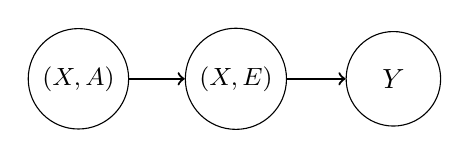
\begin{tikzpicture}

\node[circle,draw, minimum size=1.2cm] (R0) at (0,0) {\begin{small}$(X, A)$\end{small}
};
\node[circle,draw, minimum size=1.2cm] (R1) at (2,0) {\begin{small}$(X, E)$\end{small}};
\node[circle,draw, minimum size=1.2cm] (Y) at (4,0) {$Y$};

\path[->, thick] (R0) edge (R1);
\path[->, thick] (R1) edge (Y);

\end{tikzpicture}
\caption{Bayesian network corresponding to Assumption \ref{assum:indep-mips}.}
\label{fig:embedding_mips}
\vspace{-0.2cm}
% \end{wrapfigure}
\end{figure}


\myparagraph{Intuition}
The context-embedding pair $(X, E)$ can be seen as a representation of the context-action pair $(X, A)$ which contains less `redundant information' regarding the outcome $Y$. Intuitively, the MIPS estimator, which only considers the shift in the distribution of $(X, E)$ is therefore more efficient than the IPW estimator (which considers the shift in the distribution of $(X, A)$ instead). 
% In fact, as the representation $(X, E)$ gets closer to the outcome $Y$ in terms of information content, the variance of the MIPS estimator decreases. We formalise this in Appendix \faaiz{ref}. 

\myparagraph{MR achieves lower variance than MIPS}
Given the intuition above, we should achieve greater variance reduction as the amount of redundant information in the representation $(X, E)$ decreases. We formalise this in Appendix \ref{app:gmips} and show that the variance of MIPS estimator decreases as the representation gets closer to $Y$ in terms of information content. As a result, we achieve the greatest variance reduction by considering the marginal shift in the outcome $Y$ itself (as in MR) rather than the shift in the representation $(X, E)$ (as in MIPS). The following result formalizes this finding. 
% \jef{Ask Arnaud and Rob}
% As such, the greatest variance reduction is achieved when instead of considering the shift in the representation $(X, E)$ as in MIPS, we consider the marginal shift in the outcome $Y$ itself as in the MR estimator. The following results formalises this:
\begin{theorem}\label{prop:mips_main_text}
    When the weights $w(y)$, $\frac{\ptar(e, x)}{\pbeh(e, x)}$ and $\rho(a, x)$ are known exactly, then under Assumption \ref{assum:indep-mips}, 
    \begin{align*}
        \Ebeh[\thetamr] = \Ebeh[\hat{\theta}_{\textup{MIPS}}] = \Etar[Y], \quad \textup{and} \quad \Vbeh[\thetamr] \leq \Vbeh[\hat{\theta}_{\textup{MIPS}}] \leq \Vbeh[\thetaipw].
    \end{align*}
    % \[
    % \Vbeh[\thetamr] \leq \Vbeh[\hat{\theta}_{\textup{MIPS}}] \leq \Vbeh[\thetaipw].
    % \]
\end{theorem}
% \paragraph{Intuition}
This analysis provides a link between the MR and MIPS estimators in the framework of contextual bandits, and shows that the MR estimator achieves lower variance than MIPS estimator while not requiring any additional assumptions (e.g.\ Assumption \ref{assum:indep-mips} as in MIPS). We also verify this empirically in Section \ref{sec:exp-synth} by reproducing the experimental setup in \cite{saito2022off} along with the MR baseline.
% Proposition \ref{prop:mips_main_text} provides us an alternative perspective of the MR estimator. Both, the MIPS and the MR estimators lead to variance reduction by considering a representation of the context-action pair $(X, A)$ which contains less redundant information. However, in the case of the MR estimator, the representation under consideration is the outcome $Y$ itself and therefore it contains precisely the least amount of information necessary to obtain the outcome $Y$. Consequently, the variance of MR estimator is . Additionally, unlike the MIPS estimator, the MR estimator does not require any additional conditional independence assumptions.

% we replace the representation $(X, E)$ by the outcome $Y$ itself. In fact, this recovers the MR estimator.

% In fact, if instead of considering representations of 

% The intuitive reason behind the variance reduction is that the MIPS estimator considers the shift in the joint distribution of $(X, E)$ resulting from the policy shift.

\subsubsection{Weight estimation error}\label{subsec:weight-estimation-error}
% So far our analysis assumes that the behaviour policy $\beh$ and the marginal ratios $w(y)$ are known. However, in practice, both quantities may be unknown and must be estimated from data. To do so, we first split the available logged data $\D$ into training data $\Dtr = \{(x^\tr_i, a^\tr_i, y^\tr_i)\}_{i=1}^m$, which is used for weight estimation, and evaluation data $\Dev = \{(x_i, a_i, y_i)\}_{i=1}^n$, which is used to compute the OPE estimate. 
% % We then estimate the weights $w(y)$ using $\Dtr$ as follows:
% The estimation of weights $w(y)$ involves a two-step process, exclusively utilizing data from $\Dtr$ in each step:
Our analysis so far assumes prior knowledge of the behavior policy $\beh$ and the marginal ratios $w(y)$. However, in practice, both quantities are often unknown and must be estimated from data. To this end, we assume access to an additional training dataset $\Dtr = \{(x^\tr_i, a^\tr_i, y^\tr_i)\}_{i=1}^m$ (for weight estimation), in addition to the evaluation dataset $\D = \{(x_i, a_i, y_i)\}_{i=1}^n$ (for computing the OPE estimate). 
% More generally, these datasets can be obtained by splitting the available logged data.
% we first split the available logged data $\D$ into two subsets: the training data $\Dtr = \{(x^\tr_i, a^\tr_i, y^\tr_i)\}_{i=1}^m$ for weight estimation, and the evaluation data $\Dev = \{(x_i, a_i, y_i)\}_{i=1}^n$ for computing the OPE estimate.
The estimation of $\hat{w}(y)$ involves a two-step process that exclusively utilizes data from $\Dtr$:
% The weights $w(y)$ are then estimated using $\Dtr$ as follows:
% In practice, often the behaviour policy $\beh$ is not known and must be estimated through the logged observational data. 
\begin{enumerate}[label=(\roman*)]
    \item First, we estimate the policy ratio $\hat{\rho}(a, x) \approx \frac{\tar(a | x)}{\beh(a | x)}$. This can be achieved by estimating the behaviour policy $\hatbeh$, and defining $\hat{\rho}(a, x)\coloneqq \frac{\tar(a\mid x)}{\hatbeh(a\mid x)}$. Alternatively, $\hat{\rho}(a, x)$ can also be estimated directly by using density ratio estimation techniques as in \cite{sondhi2020balanced}.
    \item Secondly, we estimate the weights $\hat{w}(y)$ using Eq. \eqref{eq:weights-obj} with $\hat{\rho}$ instead of $\rho$.
\end{enumerate}

    % First, we estimate the behaviour policy $\hatbeh$, and define the policy ratio 
    % $
    % \hat{\rho}(A, X)\coloneqq \frac{\tar(a\mid x)}{\hatbeh(a\mid x)}.$
    % and use it to define the estimated ratios $\hat{\rho}(a, x)\coloneqq \tar(a\mid x)/\hatbeh(a\mid x)$.
 
% In this case, the policy ratio $\rho(a, x)$ is not known, and we resort to the use of estimated ratios $\hat{\rho}(a, x)\coloneqq \tar(a\mid x)/\hatbeh(a\mid x)$ instead.
% % This means the policy ratio $\rho(a, x)$ is not known, and must be estimated using the estimated behaviour policy, i.e.\ $\hat{\rho}(a, x)\coloneqq \tar(a\mid x)/\hatbeh(a\mid x)$. 
% The use of this ratio estimate $\hat{\rho}(a, x)$ may introduce bias in the IPW estimator. This also means that we have to rely on the estimated policy $\hatbeh$ to estimate the marginal ratio $w(y)$, which may also introduce a bias in the MR estimator. 

In practice, one may consider splitting $\Dtr$ for each estimation step outlined above. Moreover,
each approximation step may introduce bias and therefore, the MR estimator may have two sources of bias.
% the MR estimator may have two sources of bias: estimation of the behaviour policy $\hatbeh$, and the estimation of weights $\hat{w}(y)$.
% $$
% \hat{w}(y) \approx \Ebeh[\hat{\rho}(A, X)\mid Y=y] \qquad \textup{where, } \qquad  \hat{\rho}(a, x) \coloneqq \frac{\tar(a\mid x)}{\hatbeh(a\mid x)}.
% $$
While classical OPE methods like IPW and DR also suffer from bias because of $\hat{\rho}$ estimation, the estimation of $\hat{w}(y)$ is specific to MR. However, we show below
that given any policy ratio estimate $\hat{\rho}$, if $\hat{w}(y)$ approximates $\Ebeh[\hat{\rho}(A, X)\mid Y=y]$ `well enough' (i.e., the estimation step (ii) shown above is `accurate enough'), 
then MR achieves a lower variance than IPW and incurs little extra bias.

\begin{proposition}\label{prop:bias-and-var-main}
Suppose that the IPW and MR estimators are defined as,
\[
\approxipw \coloneqq \frac{1}{n}\sum_{i=1}^n\hat{\rho}(a_i, x_i)\, y_i, \quad \textup{and }\quad \approxmr \coloneqq \frac{1}{n}\sum_{i=1}^n\hat{w}(y_i)\, y_i,
\]
and define the approximation error as $\epsilon \coloneqq \hat{w}(Y) - \tilde{w}(Y)$, where $\tilde{w}(Y) \coloneqq \Ebeh[\hat{\rho}(A, X)\mid Y]$. Then we have that, $\textup{Bias}(\approxmr) - \textup{Bias}(\approxipw) = \Ebeh[\epsilon\,Y]$. Moreover,
% $\Ebeh[\epsilon] = 0$ and 
% $\epsilon \indep Y$. Then, 
% \begin{align*}
%     \textup{Bias}(\thetamr) &= \textup{Bias}(\thetaipw) \quad \textup{and,} \\
%     n (\Vbeh[\thetaipw] - \Vbeh[\thetamr]) 
%     &= \E_{Y\sim \pbeh(Y)} \left[ \Vbeh\left[ \hat{\rho}(A, X) \mid Y \right]\, Y^2 \right] - \Vbeh[\epsilon]\,\Ebeh[Y^2].
% \end{align*}
\begin{small}
\begin{align}
    \Vbeh[\approxipw] - \Vbeh[\approxmr]
    % &= \frac{1}{n}\left(\underbrace{\Ebeh[\Vbeh[\hat{\rho}(A, X)\,Y\mid Y]]}_{\geq 0} - \Vbeh[\epsilon\,Y] - 2\,\textup{Cov}(\tilde{w}(Y)\,Y, \epsilon\,Y)\right). \label{eq:var-difference-approximate-weights}
    &= \frac{1}{n}(\underbrace{\Ebeh[\Vbeh[\hat{\rho}(A, X)\,Y\mid Y]]}_{\geq 0} - \Vbeh[\epsilon\,Y] - 2\,\textup{Cov}(\tilde{w}(Y)\,Y, \epsilon\,Y)). \label{eq:var-difference-approximate-weights}
\end{align}
\end{small}
% and,
% \begin{align*}
%     &n (\Vbeh[\approxipw] - \Vbeh[\approxmr]) \\
%     &\quad= \Ebeh[\Vbeh[\hat{\rho}(A, X)\mid Y]\,Y^2] - \Vbeh[\epsilon\,Y] - 2\,\textup{Cov}(\Ebeh[\hat{\rho}(A, X)\mid Y]\,Y, \epsilon\,Y).
% \end{align*}
\end{proposition}
% if $\Ebeh[\hat{\rho}(A, X)\mid Y]$ is estimated `well enough', MR achieves a lower variance than IPW and does not incur any extra bias compared to IPW.
\myparagraph{Intuition} The $\epsilon$ term defined in Proposition \ref{prop:bias-and-var-main} denotes the error of the second approximation step outlined above. 
As a direct consequence of this result, we show in Appendix \ref{sec:wide_nns_weight_estimation} that as the error $\epsilon$ becomes small (specifically as $\Ebeh[\epsilon^2]\rightarrow 0$), the difference between biases of MR and IPW estimator becomes negligible.
% The result shows that as the error $\epsilon$ becomes small, i.e. $\epsilon \overset{\textup{a.s.}}{\rightarrow}0$, the difference between biases of MR and IPW estimator decreases. 
Likewise, the terms $\Vbeh[\epsilon\,Y]$ and $\textup{Cov}(\tilde{w}(Y)\,Y, \epsilon\,Y)$ in Eq. \eqref{eq:var-difference-approximate-weights} will also be small and as a result the variance of MR will be lower than that of IPW (as the first term is positive). 

In fact, using recent results regarding the generalisation error of neural networks \citep{lai2023generalization}, we show that when using 2-layer wide neural networks to approximate the weights $\hat{w}(y)$, the estimation error $\epsilon$ declines with increasing training data size $m$. Specifically, under certain regularity assumptions we obtain $\Ebeh[\epsilon^2] = O(m^{-2/3})$. Using this we show that as the training data size $m$ increases, the biases of MR and IPW estimators become roughly equal with a high probability, and
\[
\Vbeh[\approxipw] - \Vbeh[\approxmr] = \frac{1}{n}\,\Ebeh[\Vbeh[\hat{\rho}(A, X)\,Y\mid Y]] + O(m^{-1/3}).
\]
Therefore the variance of MR estimator falls below that of IPW for large enough $m$. The empirical results shown in Appendix \ref{subsec:mips-empirical} are consistent with this result. Due to space constraints, the main technical result has been included in Appendix \ref{sec:wide_nns_weight_estimation}.

% number of training samples $m$ increases, the biases of MR and IPW estimators become roughly equal, whereas the variance of MR estimator falls below that of the IPW estimator. The empirical results shown in Appendix \ref{subsec:additional-experiments} are consistent with this result.
% Moreover, in Theorem \ref{prop:informal}, the estimated policy ratio $\hat{\rho}(a, x)$ is fixed for increasing $m$, i.e., we do not update $\hat{\rho}(a, x)$ as more training data becomes available. While this may seem as a disadvantage for the IPW estimator, we point out that the result also holds when the policy ratio is exact (i.e., $\hat{\rho}(a, x) = \rho(a, x)$) and hence the IPW estimator is unbiased.

% In fact, using recent results regarding the generalisation error of wide neural networks \citep{lai2023generalization}, we can show that when using 2-layer wide neural networks to approximate the weights $\hat{w}(y)$, the estimation error of the second approximation step above scales as $O(m^{-1/3})$ where $m$ is the number of training data used to approximate $\hat{w}(y)$.
% % Using recent results regarding the generalisation error of wide neural networks \citep{lai2023generalization}, we show that when using 2-layer wide neural networks to approximate the weights $\hat{w}(y)$, then under mild assumptions, $\Ebeh[\epsilon^2]\leq O(m^{-2/3})$. Here $m$ is the number of training data used to approximate $\hat{w}(y)$. 
% Due to space constraints, we include an informal statement of the result here. The main technical result has been included in Appendix \ref{sec:wide_nns_weight_estimation}.

% \begin{theorem}[Informal Statement]\label{prop:informal}
% % Let $\mathcal{D}_{tr}$ be training data with $m$ samples $\{(x^\tr_i, a^\tr_i, y^\tr_i)\}_{i=1}^m$.
% Suppose that the IPW and MR estimators are defined as,
% \[
% \approxipw \coloneqq \frac{1}{n}\sum_{i=1}^n\hat{\rho}(a_i, x_i)\, y_i, \quad \textup{and }\quad \approxmr \coloneqq \frac{1}{n}\sum_{i=1}^n\hat{w}(y_i)\, y_i,
% \]
% % and let
% % \[
% % \thetamr = \frac{1}{n}\sum_{i=1}^n\hat{w}(y_i)\, y_i,
% % \]
% where $\hat{w}(y)$ is approximated by minimising the following empirical loss on a training dataset of size $m$, $\mathcal{D}_{tr}\coloneqq \{(x^\tr_i, a^\tr_i, y^\tr_i)\}_{i=1}^m$ (disjoint from evaluation dataset $\{(x_i, a_i, y_i)\}_{i=1}^n$):
% % \[
% %     \mathcal{L}(\theta) = \E_{\mathcal{D}_{tr}}(\hat{\rho}(A, X) - f_\phi(Y))^2.
% % \]
% \[
%     \mathcal{L}(\phi) = \E_{(X, A, Y)\sim \mathcal{D}_{tr}} \left[\left(\hat{\rho}(A, X) - f_{\phi}(Y)\right)^2\right].
% \]
% If $f_\phi$ is a two-layer neural network with large enough width and for sufficiently large $m$, then under the regularity assumptions provided in Appendix \ref{sec:wide_nns_weight_estimation}, the following holds with high probability,
% \begin{align*}
%     |\textup{Bias}(\approxmr) - \textup{Bias}(\approxipw)| &= O(m^{-1/3}),\\
%     \Vbeh[\approxipw] - \Vbeh[\approxmr] &= \frac{1}{n}\underbrace{\Ebeh[\Vbeh[\hat{\rho}(A, X)\mid Y]\, Y^2]}_{\geq 0} + O(m^{-2/3}).
% \end{align*}
% % holds with high probability. 
% \end{theorem}

% \myparagraph{Intuition} This theorem shows that as the number of training samples $m$ increases, the biases of MR and IPW estimators become roughly equal, whereas the variance of MR estimator falls below that of the IPW estimator. The empirical results shown in Appendix \ref{subsec:additional-experiments} are consistent with this result.
% Moreover, in Theorem \ref{prop:informal}, the estimated policy ratio $\hat{\rho}(a, x)$ is fixed for increasing $m$, i.e., we do not update $\hat{\rho}(a, x)$ as more training data becomes available. While this may seem as a disadvantage for the IPW estimator, we point out that the result also holds when the policy ratio is exact (i.e., $\hat{\rho}(a, x) = \rho(a, x)$) and hence the IPW estimator is unbiased.
 
% In this section, we show that under certain assumptions, the use of the estimated importance weights $\hat{w}(y)$ rather than $\hat{\rho}(a, x)$ does not worsen the bias of the resulting OPE estimator. Moreover, if $\hat{w}(y)$ are estimated `well enough', the variance of MR estimator will be lower than that of IPW estimator in this case as well. The following result formalises this:
% \begin{align}
%     \hat{w} = \arg\min_{f} \, \Ebeh \Bigg[\frac{\tar(A|X)}{\hatbeh (A|X)}-f(Y)\Bigg]^2, \label{eq:estimated-marginal-ratio}
% \end{align}
% then the bias in the MR estimator will be equal to the bias in the IPW estimator. This means that in the case when $\beh$ is approximated and the marginal ratio estimate $\hat{w}(y)$ are obtained by exactly regressing to the approximate policy ratios $\hat{\rho}(a, x)$, the biases of the MR and IPW estimators will be identical. Additionally, the result in Proposition \ref{prop:var_mr} straightforwardly extends to this case, showing that if the marginal ratios $\hat{w}(y)$ are estimated `well enough', the variance of MR estimator will be lower than that of IPW estimator in this case as well.

\subsection{Application to causal inference}\label{subsec:application-to-causal-inference}
 Beyond contextual bandits, the variance reduction properties of the MR estimator make it highly useful in a wide variety of other applications. Here, we show one such application in the field of causal inference, where MR can be used for the estimation of average treatment effect (ATE) \citep{pearl2009causality} and leads to some desirable properties in comparison to the conventional ATE estimation approaches. Specifically, we illustrate that the MR estimator for ATE utilizes the evaluation data $\D$ more efficiently and achieves lower variance than state-of-the-art ATE estimators and consequently provides more accurate ATE estimates.
% leads to a significantly more data efficient methodology with  
% This comparative advantage of MR becomes even more apparent when the observational data size is small.
% We show, both theoretically and empirically, that our methodology provides more reliable ATE estimation overall, and performs especially better than other baselines when the number of data is low.
% The MR estimator can also be applied in the setting of causal inference for estimation of average treatment effect (ATE) and leads to more data efficient methodology than many state-of-the-art ATE estimators.
To be concrete, the goal in this setting is to estimate ATE, defined as follows:
% Off-Policy evaluation is widely applied sin causal inference, where often the goal is to estimate the average treatment effect (ATE), defined as follows:
\[
\ate \coloneqq \E[Y(1)-Y(0)].
\]
Here $Y(a)$ corresponds to the outcome under a deterministic policy $\pi_a(a'\mid x) \coloneqq \ind(a'=a)$. Hence any OPE estimator can be used to estimate $\E[Y(a)]$ (and therefore ATE) by considering target policy $\tar = \pi_a$.
% Given an OPE estimator, $\E[Y(a)]$ 
% We can use any OPE estimator with deterministic target policies to estimate the ATE. 
% We provide explicit expressions of ATE estimators using MR, IPW and DR in Appendix \ref{app:causal-inference}.
An important distinction between MR and existing approaches (like IPW or DR) is that, when estimating $\E[Y(a)]$, the existing approaches only use datapoints in $\D$ with $A=a$. To see why this is the case, we note that the policy ratios $\frac{\tar(A|X)}{\beh(A|X)} = \frac{\ind(A=a)}{\beh(A|X)}$ are zero when $A\neq a$. In contrast, the MR weights $\frac{\ptar(Y)}{\pbeh(Y)}$ are not necessarily zero for datapoints with $A\neq a$, and therefore the MR estimator uses all evaluation datapoints when estimating $\E[Y(a)]$. 

As such we show that MR applied to ATE estimation leads to a smaller variance than the existing approaches. Moreover, because MR is able to use all datapoints when estimating $\E[Y(a)]$, MR will generally be more accurate than the existing methods especially in the setting where the data is imbalanced, i.e., the number of datapoints with $A=a$ is small for a specific action $a$.
In Appendix \ref{app:causal-inference}, we formalise this variance reduction of the MR ATE estimator compared to IPW and DR estimators, by deriving analogous results to Propositions \ref{prop:var_mr} and \ref{prop:var_dr}. In addition, we also show empirically in Section \ref{subsec:causal-experiments} that the MR ATE estimator outperforms the most commonly used ATE estimators.
\begin{comment}

\begin{proposition}\label{prop:bias-and-var}
Let 
\[
\thetaipw = \frac{1}{n}\hat{\rho}(a_i, x_i)\, y_i,
\]
where $\hat{\rho}(a, x)\coloneqq \tar(a\mid x)/\hatbeh(a\mid x)$. Additionally, let
\[
\thetamr = \frac{1}{n}\hat{w}(y_i)\, y_i,
\]
where $\hat{w}(y)$ satisfies Eq. $\eqref{eq:estimated-marginal-ratio}$. Then, 
\begin{align*}
    \textup{Bias}(\thetamr) &= \textup{Bias}(\thetaipw) \qquad \textup{and,} \\
    n (\Vbeh[\thetaipw] - \Vbeh[\thetamr]) 
    &= \E_{Y\sim \pbeh(Y)} \left[ \Vbeh\left[ \hat{\rho}(A, X) \mid Y \right]\, Y^2 \right].
\end{align*}
\end{proposition}
More generally, if $\hat{w}$ is a `noisy' estimate of the conditional expectation $\Ebeh[\hat{\rho}(A, X)\mid Y]$, we can obtain similar results regarding the bias and variance of the MR estimators under certain assumptions. 
\end{comment}


% Using recent results regarding the generalisation error of wide neural networks \citep{lai2023generalization}, we show that when using 2-layer wide neural networks to approximate the weights $\hat{w}(y)$, then under mild assumptions, $\Ebeh[\epsilon^2]\leq O(m^{-2/3})$. Here $m$ is the number of training data used to approximate $\hat{w}(y)$. Due to space constraints, we include an informal statement of the result here. The main technical result has been included in Appendix \ref{sec:wide_nns_weight_estimation}.

% Additionally, replacing the true behaviour policy $\beh$ by the estimate $\hatbeh$ in Eq. \eqref{eq:weights-obj} will 

% if we approximate the marginal ratio $w(y)$ using the approximate 



\begin{comment}
    

Specifically, the traditional IPW estimator applied to ATE estimation yields:
\[
\ateipw = \frac{1}{n} \sum_{i=1}^n \rho_{\ate}(a_i, x_i) \times y_i, \qquad \textup{where, } \qquad \rho_{\ate}(a, x) \coloneqq \frac{\mathbbm{1}(a=1) - \mathbbm{1}(a=0)}{\beh (a|x)}.
\]

Simlarly, the MR estimator can be written as
$$
\atemr = \frac{1}{n}\sum_{i=1}^n w_{\ate}(y_i)\times y_i, \qquad \textup{where, } \qquad w_{\ate}(y) = \frac{p_{\pi^{(1)}}(y) - p_{\pi^{(0)}}(y)}{\pbeh(y)},
$$ 
and $\pi^{(a)}(a'\mid x) \coloneqq \mathbbm{1}(a'=a)$ for $a\in \{0,1\}$, and $w_{\ate}(y)$ can be estimated using regression similar to Eq. \eqref{eq:weights-obj}.
\end{comment}
% Again, using the fact that $w_{\ate}(Y) \eqas \E[\rho_{\ate}(A, X)\mid Y]$, we can obtain $w_{\ate}$ by minimising a simple mean-squared loss:
% \begin{align*}
%     w_{\ate} =\arg \min_{f} \Ebeh \Big[\frac{\mathbbm{1}(A=1)- \mathbbm{1}(A=0)}{\beh (A|X)}-f(Y)\Big]^2
% \end{align*}

% For the MR estimator, we don't need to estimate weights for $Y(1)$ and $Y(0)$ separately, as we can combine the two as follows:
% \begin{align}
%     w_{\ate} =\arg \min_{f} \Ebeh \Big[\frac{\mathbbm{1}(A=1)- \mathbbm{1}(A=0)}{\beh (A|X)}-f(Y)\Big]^2 \label{eq:ate-weights-loss}
% \end{align}
% It follows straightforwardly from Lemma \ref{prop:weights-est}, that the function that minimises  \eqref{eq:ate-weights-loss} is equal to 
% \[
% w_{\ate}(y) = \frac{p_{\pi^{(1)}}(y) - p_{\pi^{(0)}}(y)}{\pbeh(y)},
% \] 
% where $\pi^{(a)}(a'\mid x) \coloneqq \mathbbm{1}(a'=a)$ for $a\in \{0,1\}$.
% Then, the MR estimator can be written as
% $$\atemr = \frac{1}{n}\sum_{i=1}^n w_{\ate}(y_i)\times y_i.$$ 
% In contrast, the traditional IPW estimator is of the form:
% \[
% \ateipw = \frac{1}{n} \sum_{i=1}^n \rho_{\ate}(a_i, x_i) \times y_i,
% \]
% where 
% \[
% \rho_{\ate}(a, x) \coloneqq \frac{\mathbbm{1}(a=1) - \mathbbm{1}(a=0)}{\beh (a|x)}.
% \]

\section{Related Work}
Off-Policy evaluation is a central problem both in contextual bandits \citep{dudik2014doubly, wang2017optimal, liu2018breaking, farajtabar2018more, su2019continuous, su2020doubly, kallus2021optimal, metelli2021subgaussian, saito2020open} and in RL \citep{thomas2016data, xie2019advances, kallus2020off, liu2020understanding}. 
Existing OPE methodologies can be broadly categorised into Direct Method (DM), Inverse Probability Weighting (IPW), and Doubly Robust (DR). 
While DM typically has a low variance, it suffers from high bias when the reward model is misspecified \citep{voloshin2021empirical}. 
On the other hand, IPW \citep{horvitz1952generalization} and DR \citep{dudik2014doubly, wang2017optimal, su2020doubly} use policy ratios as importance weights when estimating policy value and suffer from high variance as overlap between behaviour and target policies increases or as the action/context space gets larger \citep{sachdeva2020off, saito2022off}. To circumvent this problem, techniques like weight clipping or normalisation \citep{swaminathan2015counterfactual, swaminathan2015the, chaudhuri2019london} are often employed, however, these can often increase bias.

% The IPW estimator \citep{horvitz1952generalization} can have low bias but suffers from high variance as overlap between behaviour and target policies increases or as the action/context space gets larger \citep{sachdeva2020off, saito2022off}. To circumvent this problem, techniques like weight clipping or normalisation \citep{swaminathan2015counterfactual, swaminathan2015the} are often employed, however, these can often lead to the worsening of bias.



% The second class of methodologies, called the Inverse Probability Weighting (IPW) \citep{horvitz1952generalization}, uses importance weights to estimate the value of the target policy. If the behaviour policy is well-estimated, the IPW estimator will have a low bias. However, IPW can suffer from a high variance especially as the overlap between behaviour and target policies increases, or as the size of action and/or context space increases \citep{sachdeva2020off}. To circumvent this problem, techniques like weight clipping or normalisation \citep{swaminathan2015counterfactual, swaminathan2015the} are often employed, however, these can often lead to the worsening of bias. 

% The DR method \citep{dudik2014doubly} and its extensions \citep{wang2017optimal, su2020doubly} combine the direct method with importance sampling and achieves better overall bias and variance than the IPW method. However, like the IPW method these DR methods also take the shift of joint distributions of $(X, A, Y)$ into consideration when estimating policy value. As we show in Section \ref{subsec:comparison}, this can lead to high variance especially as the policy shift increases or the action and/or context space gets larger. 

In contrast to these approaches, \cite{saito2022off} propose MIPS, which considers the marginal shift in the distribution of a lower dimensional embedding of the action space. While this approach reduces the variance associated with IPW, we show in Section \ref{subsec:mips-comparison} that the MR estimator achieves a lower variance than MIPS while not requiring any additional assumptions (like Assumption \ref{assum:indep-mips}).
% it requires conditional independence assumptions on the embedding $R$, the violation of which may lead to high bias. 
% We show in Section \ref{subsec:mips-comparison} that in comparison, the MR estimator does not require any such conditional independence assumptions, and achieves a lower variance than the MIPS estimator by only considering the shift in the marginal distribution of the reward $Y$. 

In the context of Reinforcement Learning (RL), various marginalisation techniques of importance weights have been used to propose OPE methodologies.
% OPE methodologies using marginalised importance weighting have been proposed 
% \citep{liu2018breaking, xie2019advances, Fujimoto2021deep, rowland2020conditional}
% \citep{thomas2016data, xie2019advances, kallus2020off, liu2020understanding}. 
\cite{liu2018breaking, xie2019advances, kallus2020off} use methods which considers the shift in the marginal distribution of the states, and applies importance weighting with respect to this marginal shift rather than the trajectory distribution. Similarly, \cite{Fujimoto2021deep} use marginalisation for OPE in deep RL, where the goal is to consider the shift in marginal distributions of state and action. Although marginalization is a key trick of these estimators, these techniques do not consider the marginal shift in reward as in MR and are aimed at resolving the curse of horizon, a problem specific to RL. Apart from this, \cite{rowland2020conditional} propose a general framework of OPE based on conditional expectations of importance ratios for variance reduction. While their proposed framework includes reward conditioned importance ratios, this is not the main focus and there is little theoretical and empirical comparison of their proposed methodology with existing state-of-the-art methods like DR. 

Finally we note that the idea of approximating the ratio of intractable marginal densities via leveraging the fact that this ratio can be reformulated as the conditional expectation of a ratio of tractable densities is a standard idea in computational statistics \cite{meng1996simulating} and has been exploited more recently to perform likelihood-free inference \cite{brehmer2020mining}. In particular, while  \cite{meng1996simulating} typically approximates this expectation through Markov chain Monte Carlo, \cite{brehmer2020mining} uses regression instead, however without any theory.
% of this approach has been carried out in \cite{brehmer2020mining}.

% Our work introduces the marginal ratio estimator for OPE in contextual bandits. We provide extensive theoretical and empirical comparisons of our proposed estimator with existing methods, and show that the MR estimator performs especially better than the other methods in large actions and/or context spaces. 
% \faaiz{@Arnaud and Rob: what are your thoughts about this characterisation of \cite{rowland2020conditional}?}

% Our work proposes an OPE methodology for contextual bandits which only considers the shift in the marginal distribution of rewards. In addition, we include extensive theoretical and empirical comparisons of our proposed estimator with existing methods, and show that the MR estimator performs especially better than the other methods in large actions and/or context spaces. 

\begin{comment}
\begin{itemize}
    \item IPW
    \item Double robust methods
    \item Debiased methods 
    \item See related works in \cite{saito2022off}
\end{itemize}
\subsection{Baselines in Contextual Bandits setting}
\begin{itemize}
    \item \cite{thomas2016data, saito2021evaluating, saito2022off,wang2017optimal}
    \item Using ideas from \cite{saito2022off},  we can show that our methodology requires common support of $\pbeh(Y\mid X)$ and $\ptar(Y\mid X)$ which is weaker than requiring common supports of $\beh(A\mid X)$ and $\tar(A\mid X)$, which is needed for IPW estimator. We can show that our estimator has a smaller variance than the methodology proposed by \cite{saito2022off}. Moreover, we should show empirically that, as a consequence of this, our estimator is more robust to heavy-tailed policy ratios. The baselines considered in this paper are the ones to compare against.
    \item \cite{wang2017optimal} proposes a SWITCH estimator for policy evaluation, and show that this estimator is minimax optimal when the hyperparameter $\tau$ is chosen appropriately. Moreover, this estimator is more robust to large (or heavy-tailed) importance weights. It also includes an expression for the variance of the DR estimator which could be useful.
    \item \cite{saito2021evaluating}: In this work, the authors develop Interpretable Evaluation for Offline Evaluation (IEOE), an experimental procedure to evaluate OPE estimators’ robustness to changes in hyperparameters and/or evaluation policies in an interpretable manner. This is more of a review paper.
    \item \cite{liu2019triply}: Could be an interesting baseline. The background section of this paper seems interesting. 
\end{itemize}
\subsection{Marginalised Importance Sampling in Reinforcement Learning}
The main difference between this line of work and our idea is that these works consider the marginal distribution over the states. Instead, we propose considering the marginal distribution over rewards directly. 
\begin{itemize}
    \item \cite{liu2018breaking}: The paper originally proposed avoiding the long horizon problem by computing MIS over state distributions rather than entire trajectories. The marginal ratio in these works is different to ours.  
    \item \cite{Fujimoto2021deep}: Applies the MIS idea to deep RL setting: Marginalized importance sampling (MIS), which measures the density ratio between the state-action occupancy of a target policy and that of a sampling distribution, is a promising approach for off-policy evaluation. However, current state-of-the-art MIS methods rely on complex optimization tricks and succeed mostly on simple toy problems. This paper bridges the gap between MIS and deep reinforcement learning by observing that the density ratio can be computed from the successor representation of the target policy. 
    \item \cite{kallus2020off}: The related works section of this paper is very useful. In this work, the authors propose the use of a marginal importance sampling estimator which is somewhat similar to ours (although not the same). Would be useful to read this in depth.
    \item \cite{xie2019advances}: Avoiding the long horizon problem by computing IS over state distributions rather than trajectories - was already introduced in \cite{liu2018breaking}, which the authors cite sufficiently often in the text. However, the approach the authors take to leveraging this idea is original. The estimation technique for the ratios is also different -- the authors propose a recursive estimation technique to estimate the marginal distribution ratios over states. 
    \item \cite{liu2020understanding} also references MIS estimators. 
    \item \cite{rowland2020conditional}: This paper proposes conditional importance sampling for variance reduction in RL setting. The paper considers a general conditioning strategy, based on conditioning importance weights on different statistics. They also mention reward conditional importance sampling. \textbf{Important paper.} 
\end{itemize}
\end{comment}


\section{Empirical Evaluation}
In this section, we provide empirical evidence to support our theoretical results by investigating the performance of our MR estimator against the current state-of-the-art OPE methods. The code to reproduce our experiments has been made available at: \href{https://github.com/faaizT/MR-OPE}{\textcolor{blue}{github.com/faaizT/MR-OPE}}.
% Here, we present a synthetic data experiment and also consider an application of MR to causal inference. 
% Additional experiments that support our proposed method MR on real-world classification datasets are provided in Appendix \ref{app:experiments} due to space constraints. \faaiz{Squeeze in classification exps in main}
% We first consider a synthetic setup to conduct extensive ablation study
% We evaluate MR estimator on synthetic data to identify the cases where it offers more accurate off-policy evaluation. These experiments are conducted using the \emph{OpenBanditPipeline} (OBP)
% % \footnote{\url{https://github.com/st-tech/zr-obp}}
% , an open-source package for OPE developed by \cite{saito2020open}.

\subsection{Experiments on synthetic data}\label{sec:exp-synth}
For our synthetic data experiment, we reproduce the experimental setup for the synthetic data experiment in \cite{saito2022off} by reusing their code with minor modifications.
% We use synthetically generated dataset for this experiment. 
Specifically, $\Xspace \subseteq \mathbb{R}^d$, for various values of $d$ as described below. Likewise, the action space $\Aspace = \{0, \dots, n_a-1\}$, with $n_a$ taking a range of different values. Additional details regarding the reward function, behaviour policy $\beh$, and the estimation of weights $\hat{w}(y)$ have been included in Appendix \ref{subsec:mips-empirical} for completeness. 

% $d$-dimensional context vectors $x$ are sampled from a standard normal distribution, i.e.\ $\Xspace \subseteq \mathbb{R}^d$, for various values of $d$ as described below. Likewise, the action space is finite and comprises of $n_a$ actions, i.e.\ $\Aspace = \{0, \dots, n_a-1\}$, with $n_a$ taking a range of different values. 
% Due to space constraints, we include additional details regarding the reward function, behaviour policy $\beh$, and the estimation of weights $\hat{w}(y)$ in Appendix \ref{sec:app-additional-results}. 


\myparagraph{Target policies} 
To investigate the effect of increasing policy shift, we define a class of policies,
\[
% \vspace{-0.05cm}
\pi^{\alpha^\ast}(a | x) = \alpha^\ast\,\ind(a = \arg\max_{a'\in \Aspace} q(x, a')) + \frac{1-\alpha^\ast}{|\Aspace|} \quad \textup{where} \quad q(x, a) \coloneqq \E[Y\mid X=x, A=a],
% \vspace{-0.05cm}
\]
where $\alpha^\ast \in [0, 1]$ allows us to control the shift between $\beh$ and $\tar$. In particular, as we show later, the shift between $\beh$ and $\tar$ increases as $\alpha^\ast \rightarrow 1$. Using the ground truth behaviour policy $\beh$, we generate a dataset which is split into training and evaluation datasets of sizes $m$ and $n$ respectively. 


% \paragraph{Reward function}
% The expected reward $q(x, a)\coloneqq\E[Y\mid x, a]$ for these experiments is defined as follows:
% \[
%     q(x, a) = \sin \left(a \cdot ||x||_2 \right). 
% \]
% The reward $Y$ is obtained by adding a normal noise random variable to $q(x, a)$
% \[
% Y = q(X, A) + \epsilon, 
% \]
% where $\epsilon \sim \mathcal{N}(0, 0.01)$.

% \paragraph{Behaviour and target policies}
% We first define a behaviour policy by applying softmax function to $q(x, a)$ as
% \[
% \beh(a\mid x) = \frac{\exp{(q(x, a))}}{\sum_{a' \in \Aspace} \exp{(q(x, a'))}}.
% \]

% where $\beta$ controls the optimality and entropy of the policy $\pi_\beta$. A large positive value of $\beta$ leads to a near-deterministic and well-performing policy, while lower values make the policy increasingly worse and `noisy'. 
% In this experiment, we define the behaviour policy as $\beh = \pi_{\beta^b}$ for $\beta^b = 0.5$ and target policies as $\tar= \pi_{\beta^\ast}$ for $\beta^\ast \in \{0.0, 0.5, 1.0, \ldots, 5.0 \}$.
% In contrast, for the target policy, we define the class of parametric policies,
% \[
% \pi^{\alpha^\ast}(a | x) = \alpha^\ast\,\ind(a = \arg\max_{a'\in \Aspace} q(x, a')) + \frac{1-\alpha^\ast}{|\Aspace|},
% \]
% where $\alpha^\ast \in [0, 1]$ controls the quality of $\pi^{\alpha^\ast}$. In particular, as $\alpha^\ast \rightarrow 1$, the target policy approaches the optimal policy. 


\myparagraph{Baselines} 
We compare our estimator with DM, IPW, DR and MIPS estimators. Our setup includes action embeddings $E$ satisfying Assumption \ref{assum:indep-mips}, and so MIPS is unbiased.
% Since there is no natural action embedding $E$ in our setup which satisfies Assumption \ref{assum:indep-mips}, we instead consider a generalised version of MIPS (defined as G-MIPS in Appendix \ref{app:gmips}) which uses an embedding of context-action pair $(X, A)$ rather than an embedding of the action $A$.
% \footnote{We also compare against the original MIPS estimator in Appendix \ref{subsec:mips-empirical} by reproducing the setup of \cite{saito2022off}}
Additional baselines have been considered in Appendix \ref{subsec:mips-empirical}.
For MR, we split the training data to estimate $\hatbeh$ and $\hat{w}(y)$, whereas for all other baselines we use the entire training data to estimate $\hatbeh$ for a fair comparison.
% In addition, we also consider Switch-DR \citep{wang2017optimal} and DR with Optimistic Shrinkage (DRos) \citep{su2020doubly}. 
% To estimate $\hat{q}(x, a)$ for DM and DR estimators, we use multi-layer perceptrons (MLPs). \jef{last sentence not needed}
% \jef{I personally think having the legend at the top is better as now it is asymetric ... not a big deal though lol (fig2)
% }
\begin{figure}[t]
     \centering
     \begin{subfigure}[b]{0.5\textwidth}
         \centering
         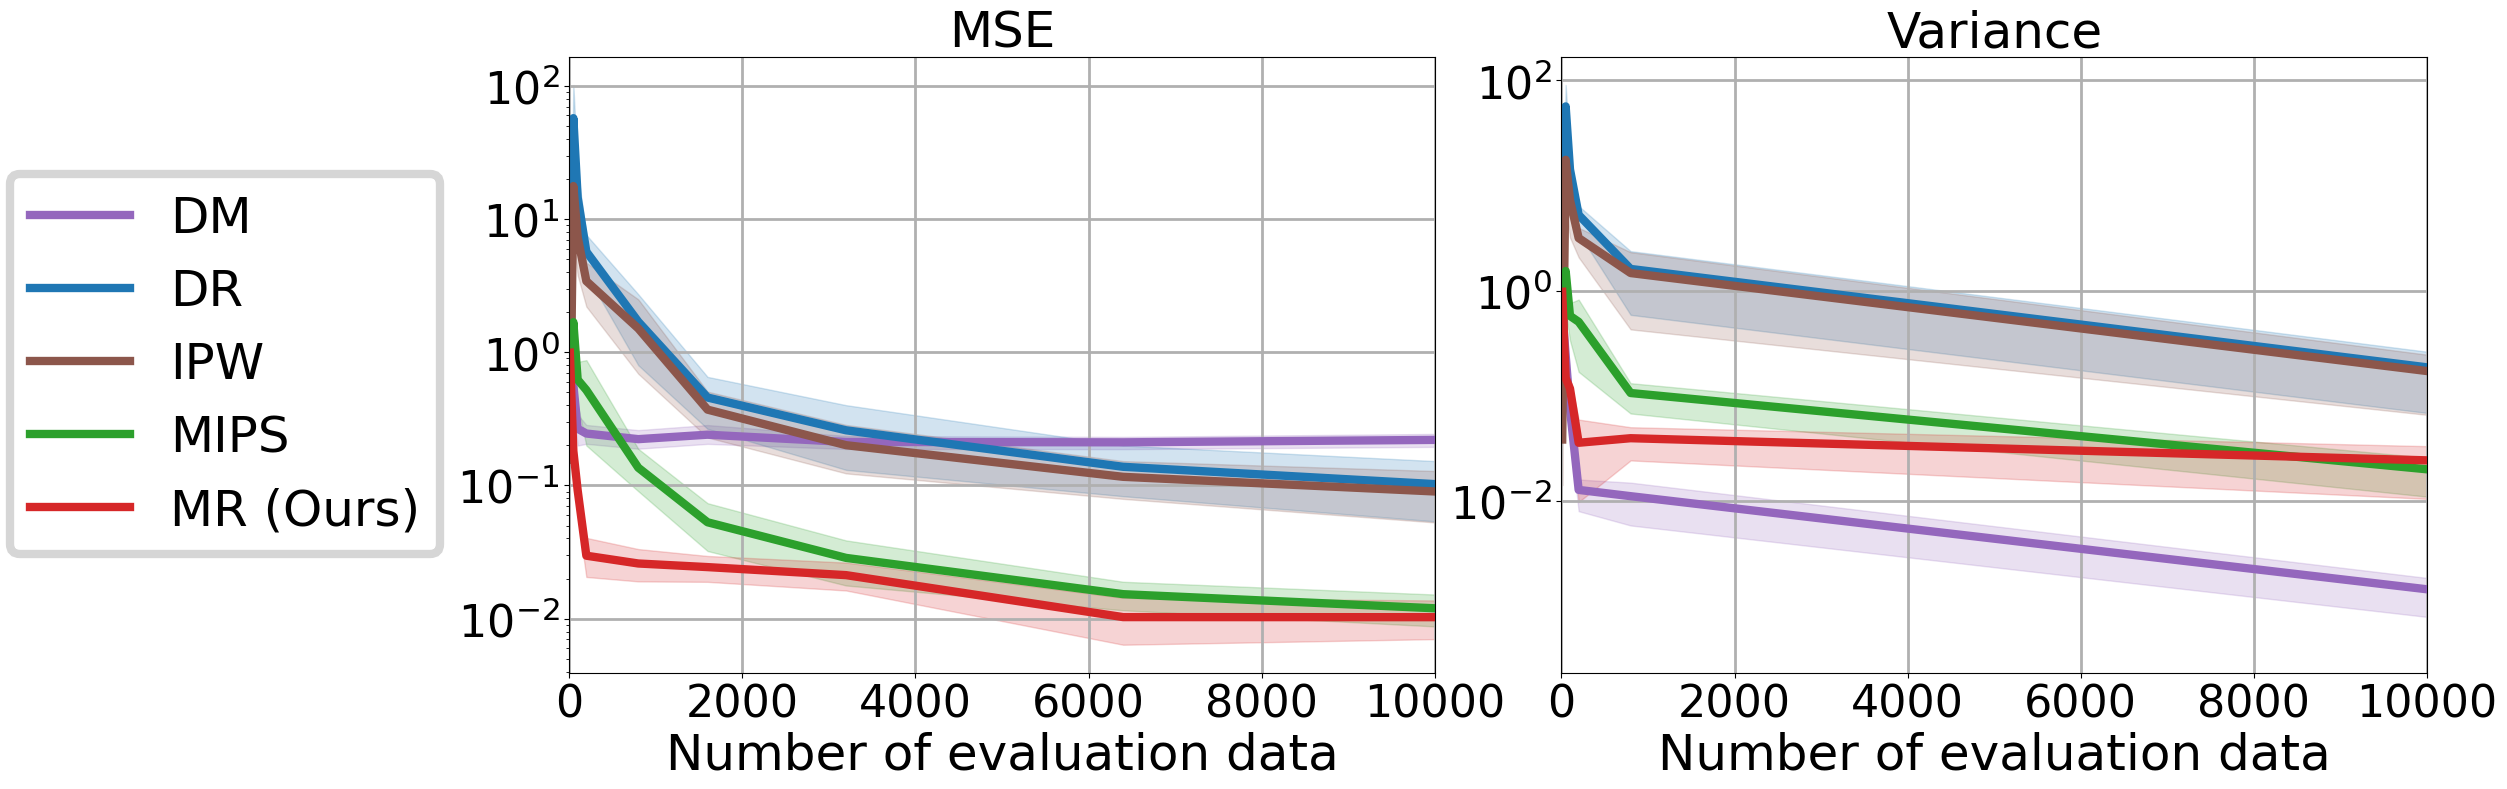
\includegraphics[height=1.06in]{figures/mr/ope_vs_neval_nac_100_alphatar_0_8_dimc_1000_untrunc.png}
         \caption{Results with varying evaluation data size $n$.}
         \label{fig:mse-vs-neval}
     \end{subfigure}%
     \begin{subfigure}[b]{0.5\textwidth}
         \centering
         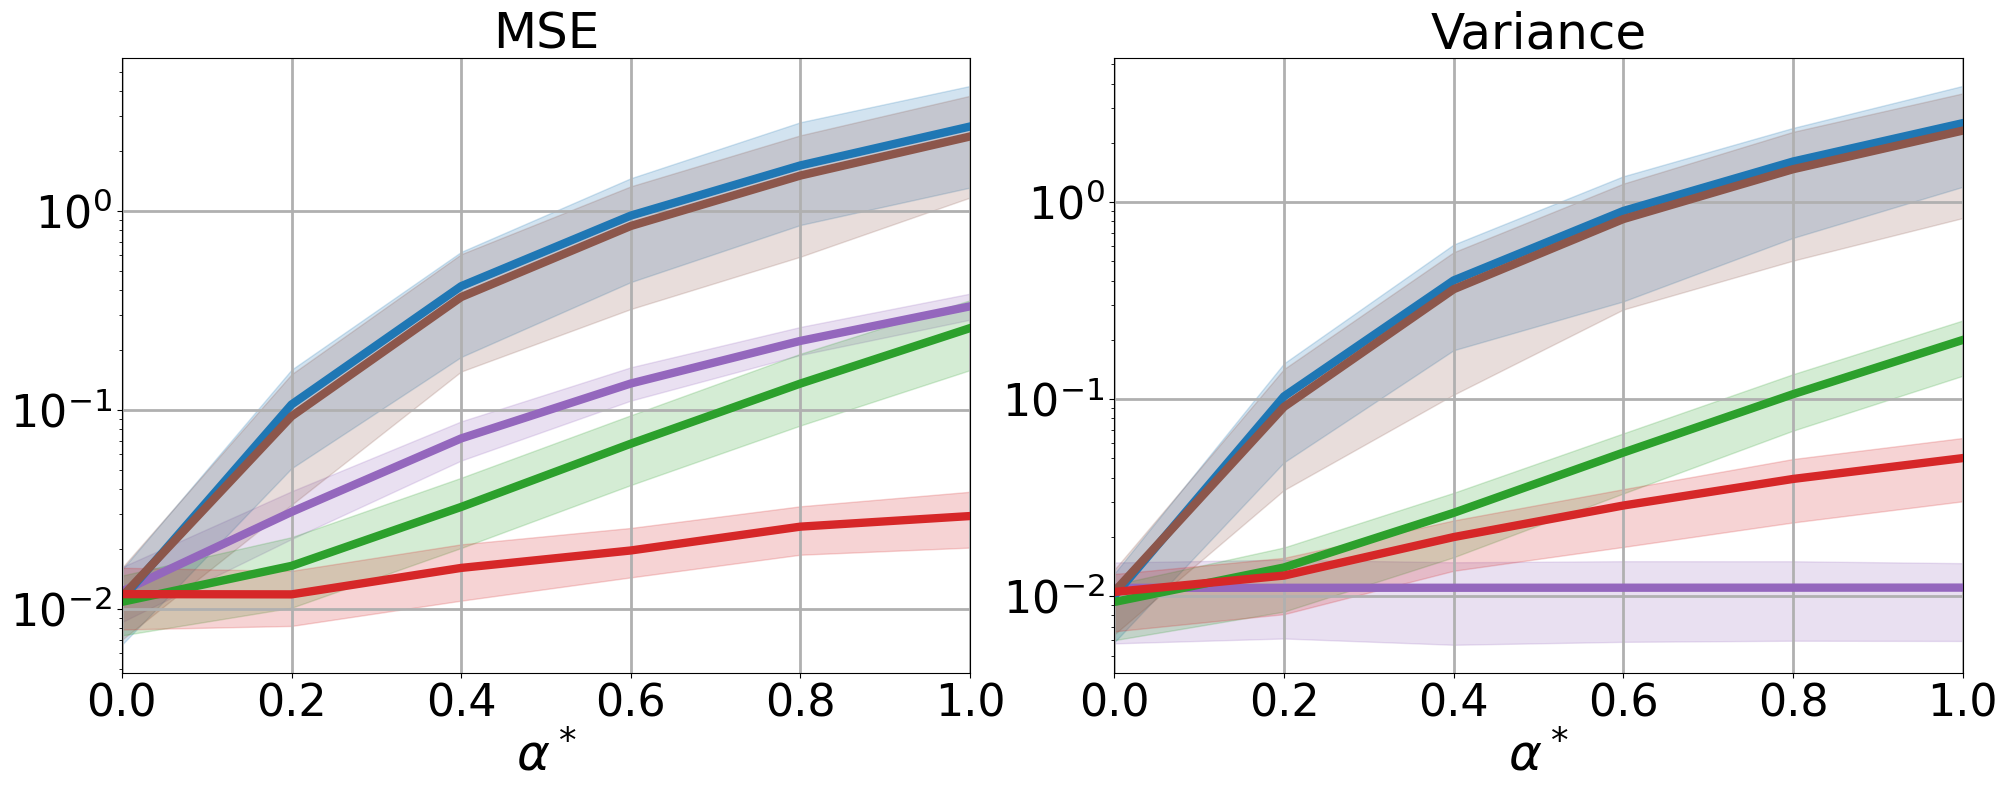
\includegraphics[height=1.06in]{figures/mr/ope_vs_alphatar_nac_100_neval_800_dimc_1000.png}
         \caption{Results with varying $\alpha^\ast$.}
         \label{fig:mse-vs-betatar}
     \end{subfigure}\\
    \caption{Results for synthetic data experiment. In \ref{fig:mse-vs-neval} we have $\alpha^\ast=0.8$ and in \ref{fig:mse-vs-betatar} we have $n = 800$.}
    \label{fig:syn_results1}
\end{figure}

% \begin{figure}[t]
%      \centering
%      \begin{subfigure}[b]{1\textwidth}
%          \centering
%          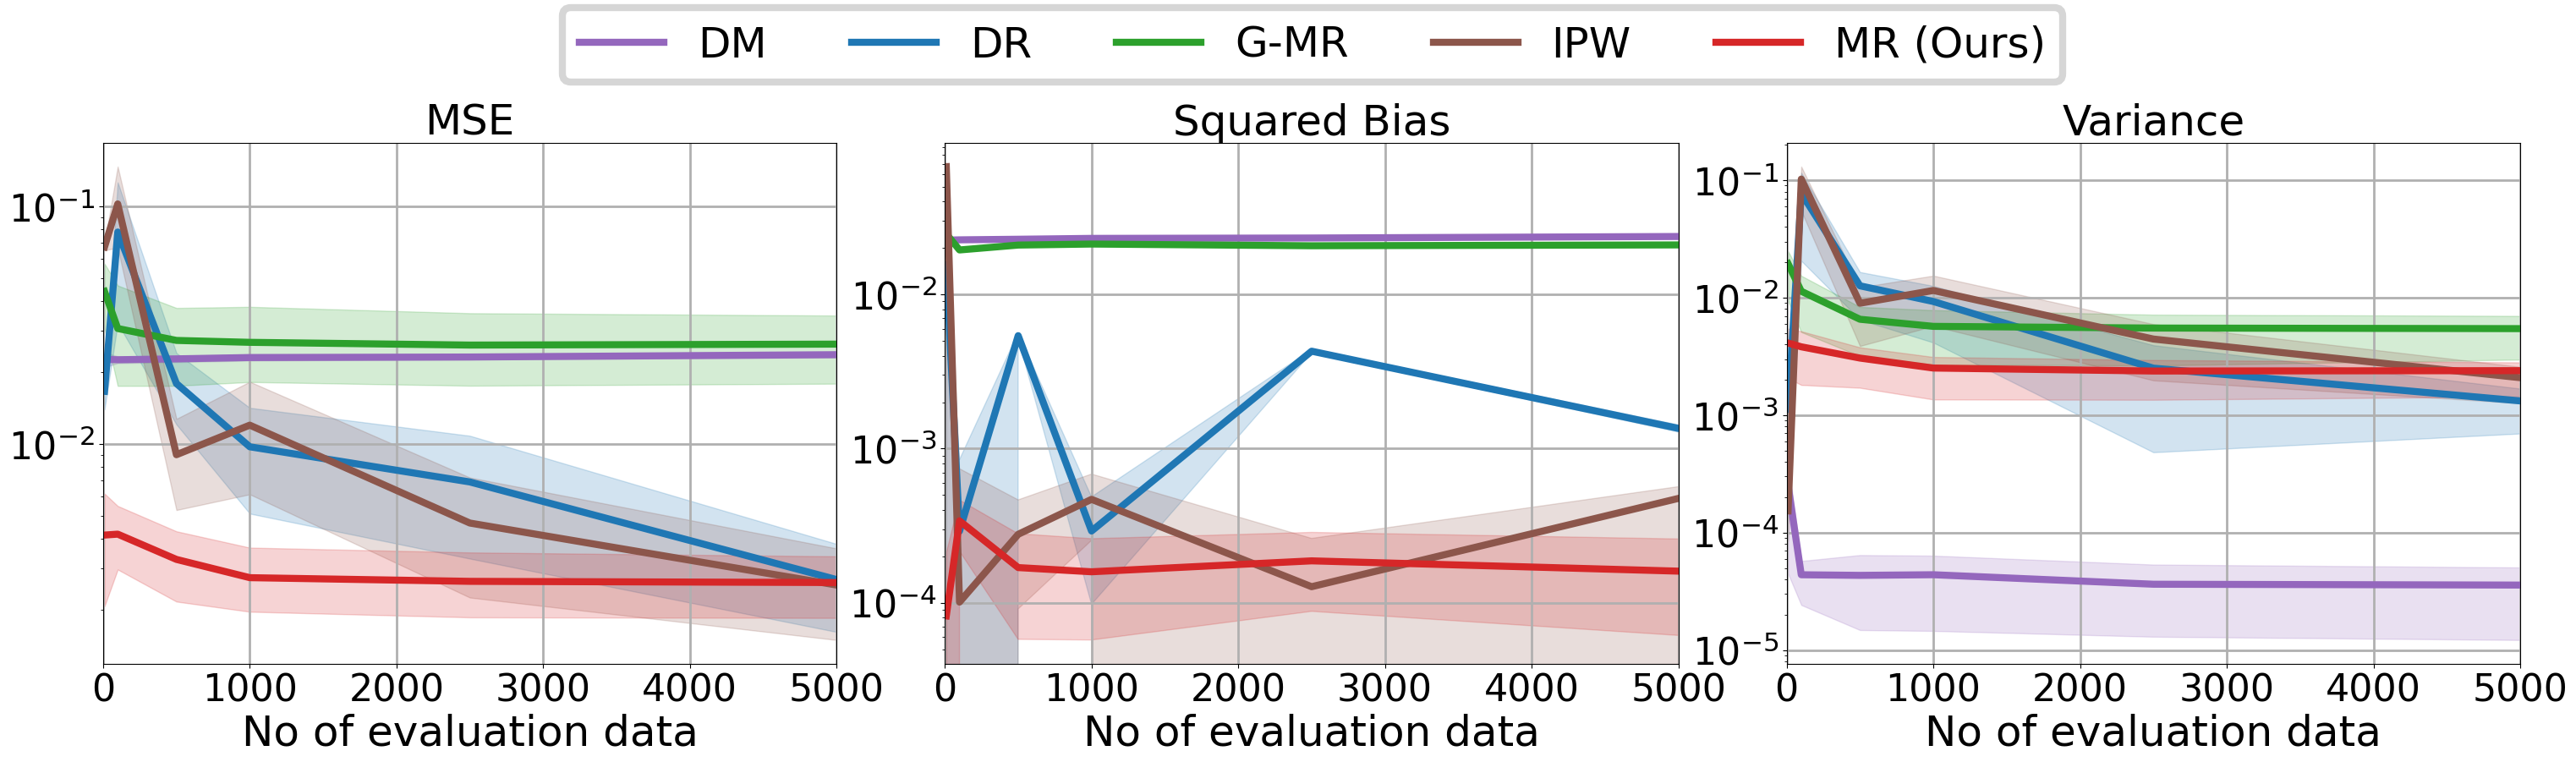
\includegraphics[width=0.75\textwidth]{figures/mr/ope_vs_neval_nac_100_alphatar_0_8_dimc_100_ntrain_100000.png}
%          \caption{Results with varying size of evaluation dataset $n$ for $\alpha^\ast = 0.8$.}
%          \label{fig:mse-vs-neval}
%      \end{subfigure}\\
%      \begin{subfigure}[b]{1\textwidth}
%          \centering
%          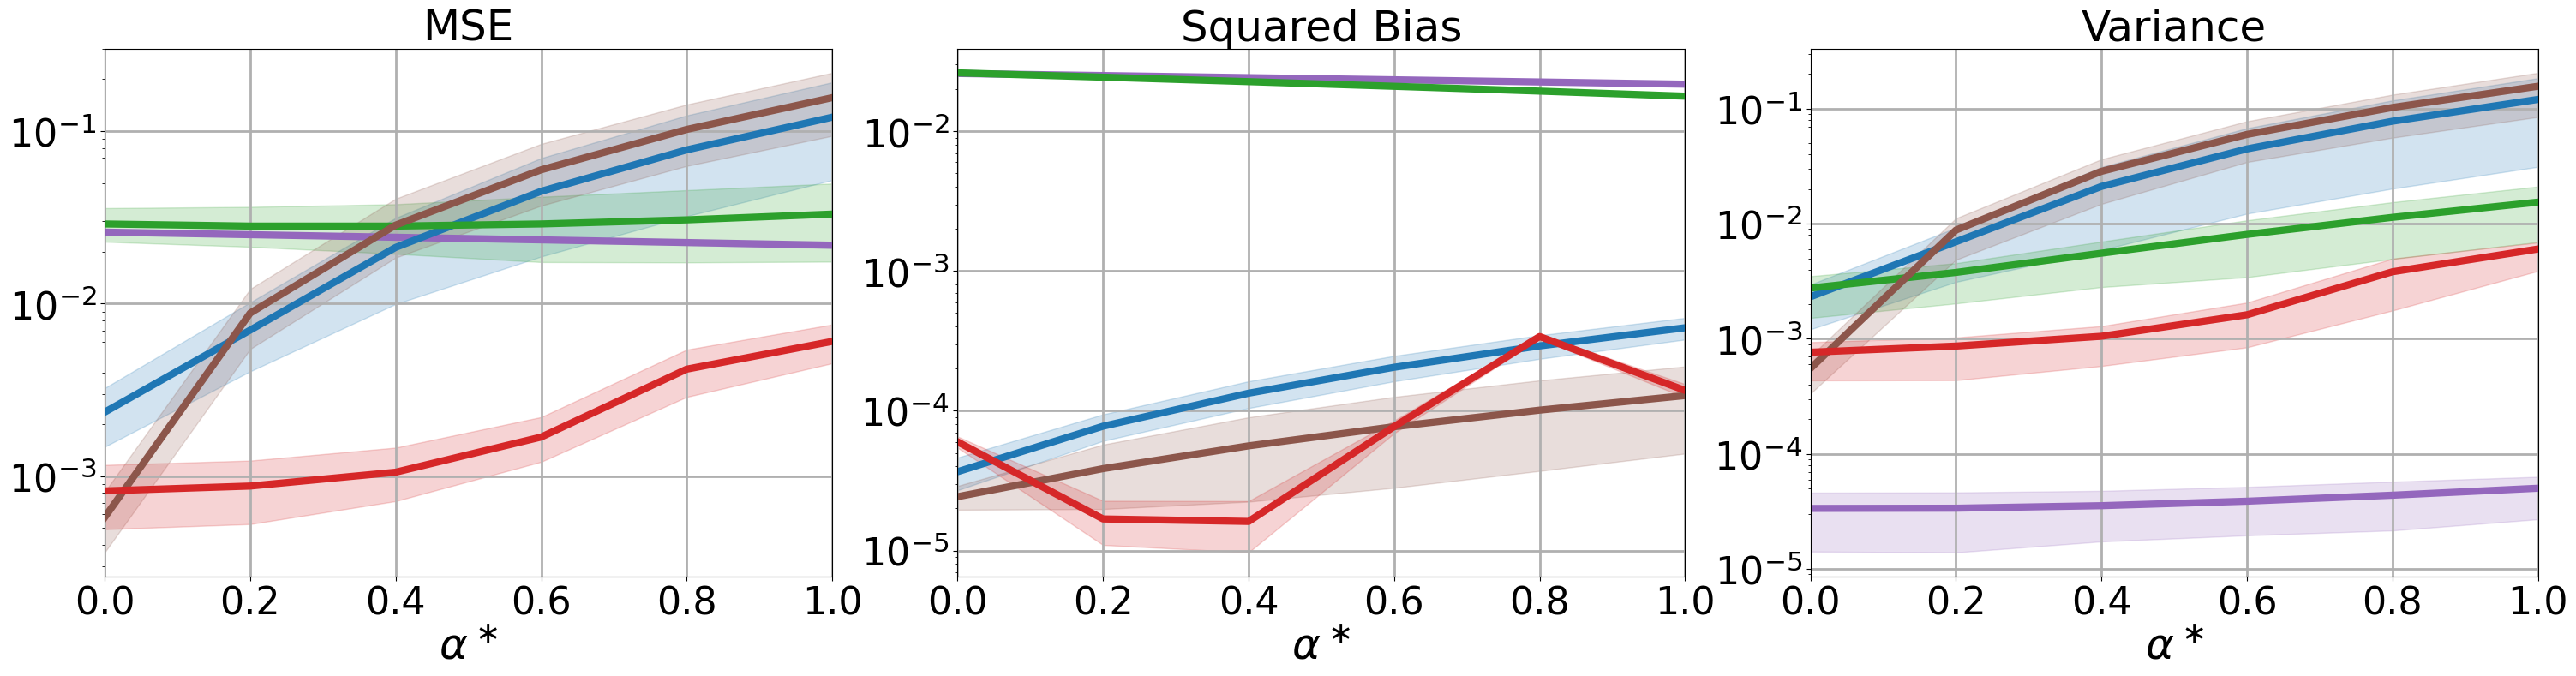
\includegraphics[width=0.75\textwidth]{figures/mr/ope_vs_alphatar_nac_100_neval_100_dimc_100_ntrain_100000.png}
%          \caption{Results with varying $\alpha^\ast$ for $n = 100$.}
%          \label{fig:mse-vs-betatar}
%      \end{subfigure}\\
%     \caption{Results with increasing $n$ and $\alpha^\ast$.}
%     \label{fig:syn_results1}
% \end{figure}
\myparagraph{Results}
We compute the target policy value using the $n$ evaluation datapoints. Here, the MSE of the estimators is computed over 10 different sets of logged data replicated with different seeds. The results presented have context dimension $d=1000$, number of actions $n_a=100$ and training data size $m=5000$. More experiments for a variety of parameter values are included in Appendix \ref{subsec:mips-empirical}.


% \begin{figure}
%      \centering
%      \begin{subfigure}[b]{1\textwidth}
%          \centering
%          \includegraphics[width=\textwidth]{figures/mr/latest/ope_vs_neval_nac_100_alphatar_0.2_dimc_100_ntrain_100000.png}
%          \caption{Results with varying size of evaluation dataset $n$ for $d=100$, $n_{a}=100$, $\alpha^\ast = 0.2$.}
%          \label{fig:mse-vs-neval}
%      \end{subfigure}\\
%      \begin{subfigure}[b]{1\textwidth}
%          \centering
%          \includegraphics[width=\textwidth]{figures/mr/latest/ope_vs_alphatar_dimc_100_nac_100_neval_100_ntrain_10000.png}
%          \caption{Results with varying $\alpha^\ast$ for $d=100$, $n_{a}=100$, $n = 100$.}
%          \label{fig:mse-vs-betatar}
%      \end{subfigure}\\
%      \begin{subfigure}[b]{1\textwidth}
%          \centering
%          \includegraphics[width=\textwidth]{figures/mr/latest/ope_vs_dimc_nac_100_alphatar_0.2_neval_100_ntrain_100000.png}
%          \caption{Results with varying context dimensions $d$ for $n_{a}=100$, $n = 100$, $\alpha^\ast = 0.2$.}
%          \label{fig:mse-vs-d}
%      \end{subfigure}\\
%      \begin{subfigure}[b]{1\textwidth}
%          \centering
%          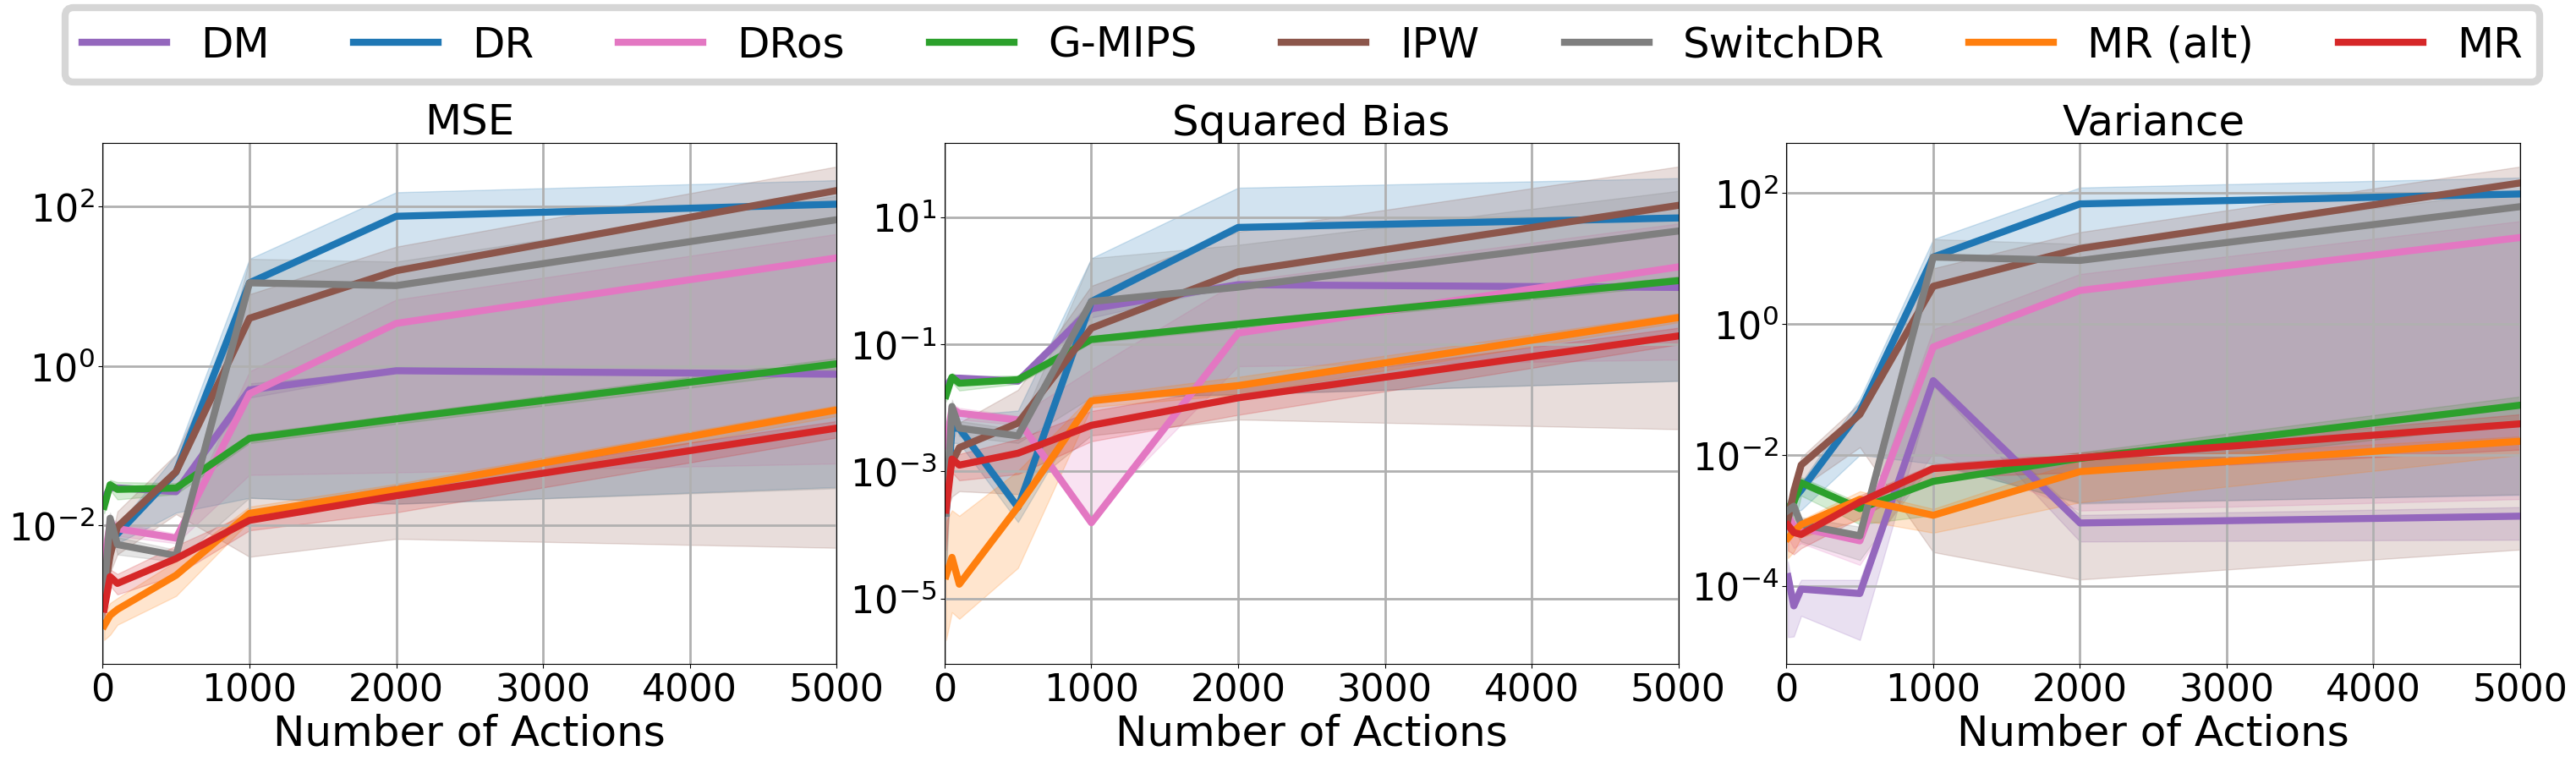
\includegraphics[width=\textwidth]{figures/mr/latest/ope_vs_nac_dimc_100_alphatar_0.2_neval_100_ntrain_100000.png}
%          \caption{Results with varying number of actions $n_{a}$ for $d=100$, $n = 100$, $\alpha^\ast = 0.2$.}
%          \label{fig:mse-vs-nac}
%      \end{subfigure}
%         \caption{Results for synthetic data experiments}
%         \label{fig:syn_results}
% \end{figure}

\myparagraph{Varying number of evaluation data $n$} 
In Figure \ref{fig:mse-vs-neval} we plot the results with increasing size of evaluation data $n$ increases. MR achieves the smallest MSE among all the baselines considered when $n$ is small, with the MSE of MR being at least an order of magnitude smaller than every baseline for $n\leq 500$. This shows that MR is significantly more accurate than the baselines when the size of the evaluation data is small. As $n\rightarrow \infty$, the difference between the results for MR and MIPS decreases. However, MR attains smaller variance and MSE than MIPS generally, verifying our analysis in Section \ref{subsec:mips-comparison}.
% IPW and DR become increasingly accurate because of their consistency and therefore the difference between MR and these baselines becomes less pronounced. 
% Additionally, it can be seen that the MR estimator also achieves the smallest squared bias overall. 
% In contrast, G-MR has a high squared bias as a result of the estimation error of the marginal ratio $\ptar(r)/\pbeh(r)$, which is more difficult to estimate the marginal ratio $\ptar(y)/\pbeh(y)$ as $r$ is two dimensional. The variance of G-MR estimator, on the other hand, is smaller than that of IPW when $n < 2000$, as suggested by Proposition \ref{prop:mips_var_reduction}.
Moreover, Figure \ref{fig:mse-vs-neval} shows that while the variance of MR is greater than that of DM, it still achieves the lowest MSE overall, owing to the high bias of DM.

\begin{wrapfigure}{r}{0.35\textwidth}
    \centering
    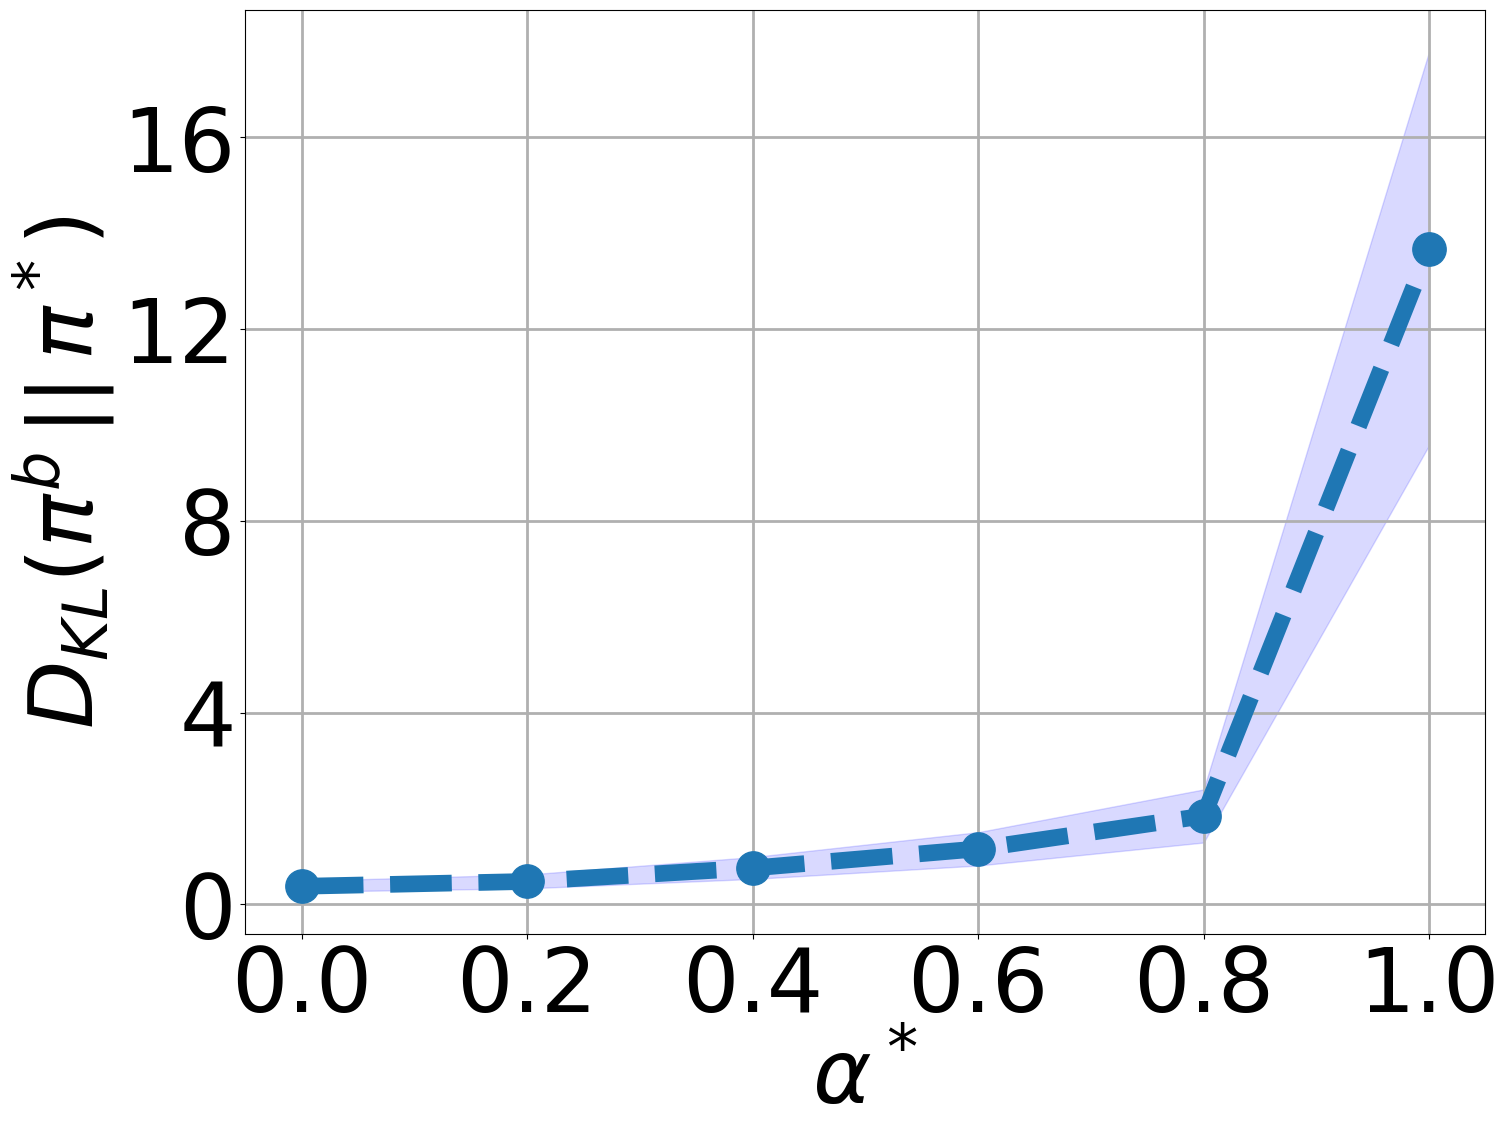
\includegraphics[width=0.35\textwidth]{figures/mr/kl-divergence-w-uncertainty.png}
    % \vspace{-0.75cm}
    % \caption{$D_{\textup{KL}}(\beh \,||\, \tar)$ with increasing $\alpha^\ast$}
    % \label{fig:kl-div-synthetic-data}
\end{wrapfigure}
\myparagraph{Varying $\alpha^\ast$}
As $\alpha^\ast$ parameter of the target policy increases, so does the shift between the policies $\beh$ and $\pi^{\alpha^\ast}$ as illustrated by the figure on the right, which plots the KL-divergence $D_{\textup{KL}}(\beh\, || \, \pi^{\alpha^\ast})$ as a function of $\alpha$.
% To analyse the shift between the policies $\beh$ and $\pi^{\alpha^\ast}$, the figure on the right plots the KL-divergence between the two policies as $\alpha^\ast$ increases. 
% \ref{fig:kl-div-synthetic-data}. 
% The figure shows that the shift between target and behaviour policies increases with increasing $\alpha^\ast$.
Figure \ref{fig:mse-vs-betatar} plots the results for increasing policy shift. 
Overall, the MSE of MR estimator is lowest among all the baselines. Moreover, while the MSE and variance of all estimators increase with increasing $\alpha^\ast$ the increase in these quantities is lower for the MR estimator than for the other baselines. Therefore, the relative performance of MR estimator improves with increasing policy shift and MR remains robust to increase in policy shift.
% It can be seen that the MSE of MR remains roughly the same with increasing $\alpha^\ast$, whereas the MSE of all other baselines increases. Moreover, both the squared bias and variance of the MR estimator becomes comparatively better than those of other baselines as the policy shift increases. 
% While the MSE and variances of all baselines increases with increasing $\beta^\ast$, the MSE and variance of MR estimator remains relatively small. Moreover, while the MSE of DM does not change noticeably with changing  $\beta^\ast$, it is still at least 2 orders of magnitude larger than that of MR. 
% This shows that MR remains significantly robust to increase in policy shift, relative to the other baselines.

\myparagraph{Additional ablation studies}
In Appendix \ref{subsec:mips-empirical}, we investigate the effect of varying context dimensions $d$, number of actions $n_a$ and number of training data $m$. In every case, we observe that the MR estimator has a smaller MSE than all other baselines considered. In particular, MR remains robust to increasing $n_a$ whereas the MSE and variance of IPW and DR estimators degrade substantially when $n_a \geq 2000$. Likewise, MR outperforms the baselines even when the training data size $m$ is small.

% \begin{figure}[t]
%      \centering
%      \begin{subfigure}[b]{0.5\textwidth}
%          \centering
%          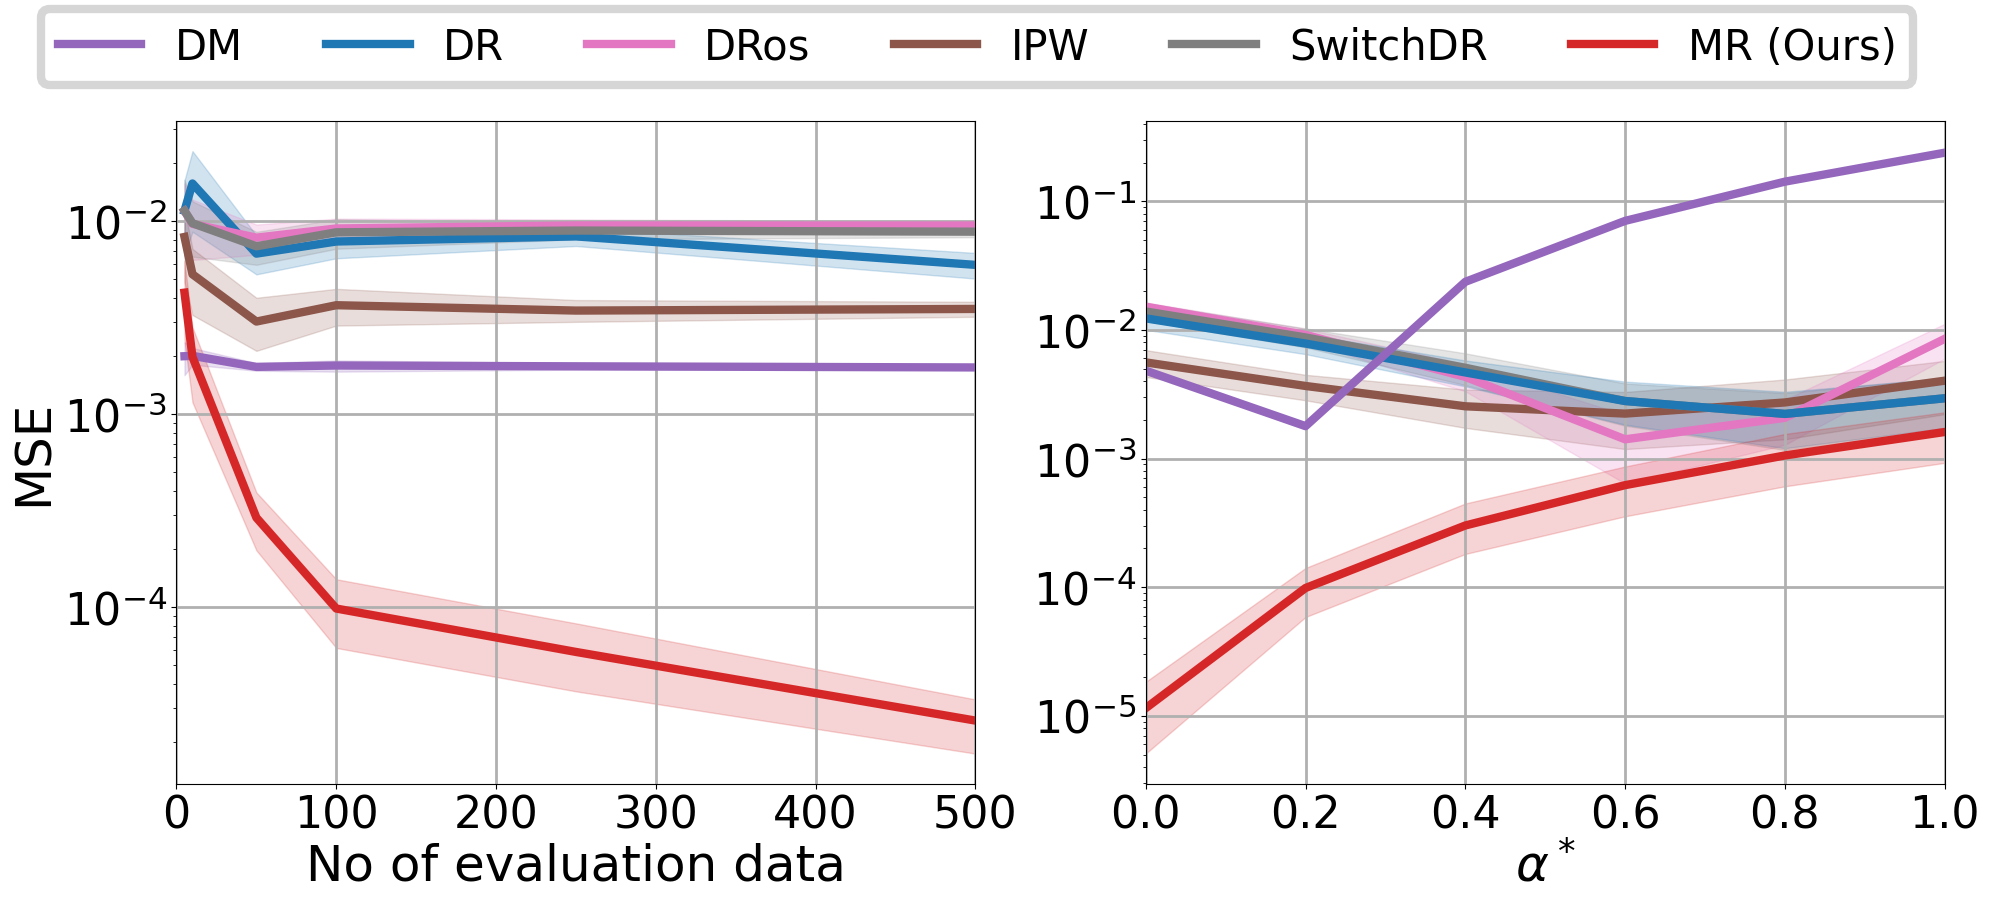
\includegraphics[height=0.92in]{figures/mr/pendigits_main.png}
%          \caption{Results for PenDigits dataset}
%          \label{fig:pendigits-main}
%      \end{subfigure}%
%      \begin{subfigure}[b]{0.5\textwidth}
%          \centering
%          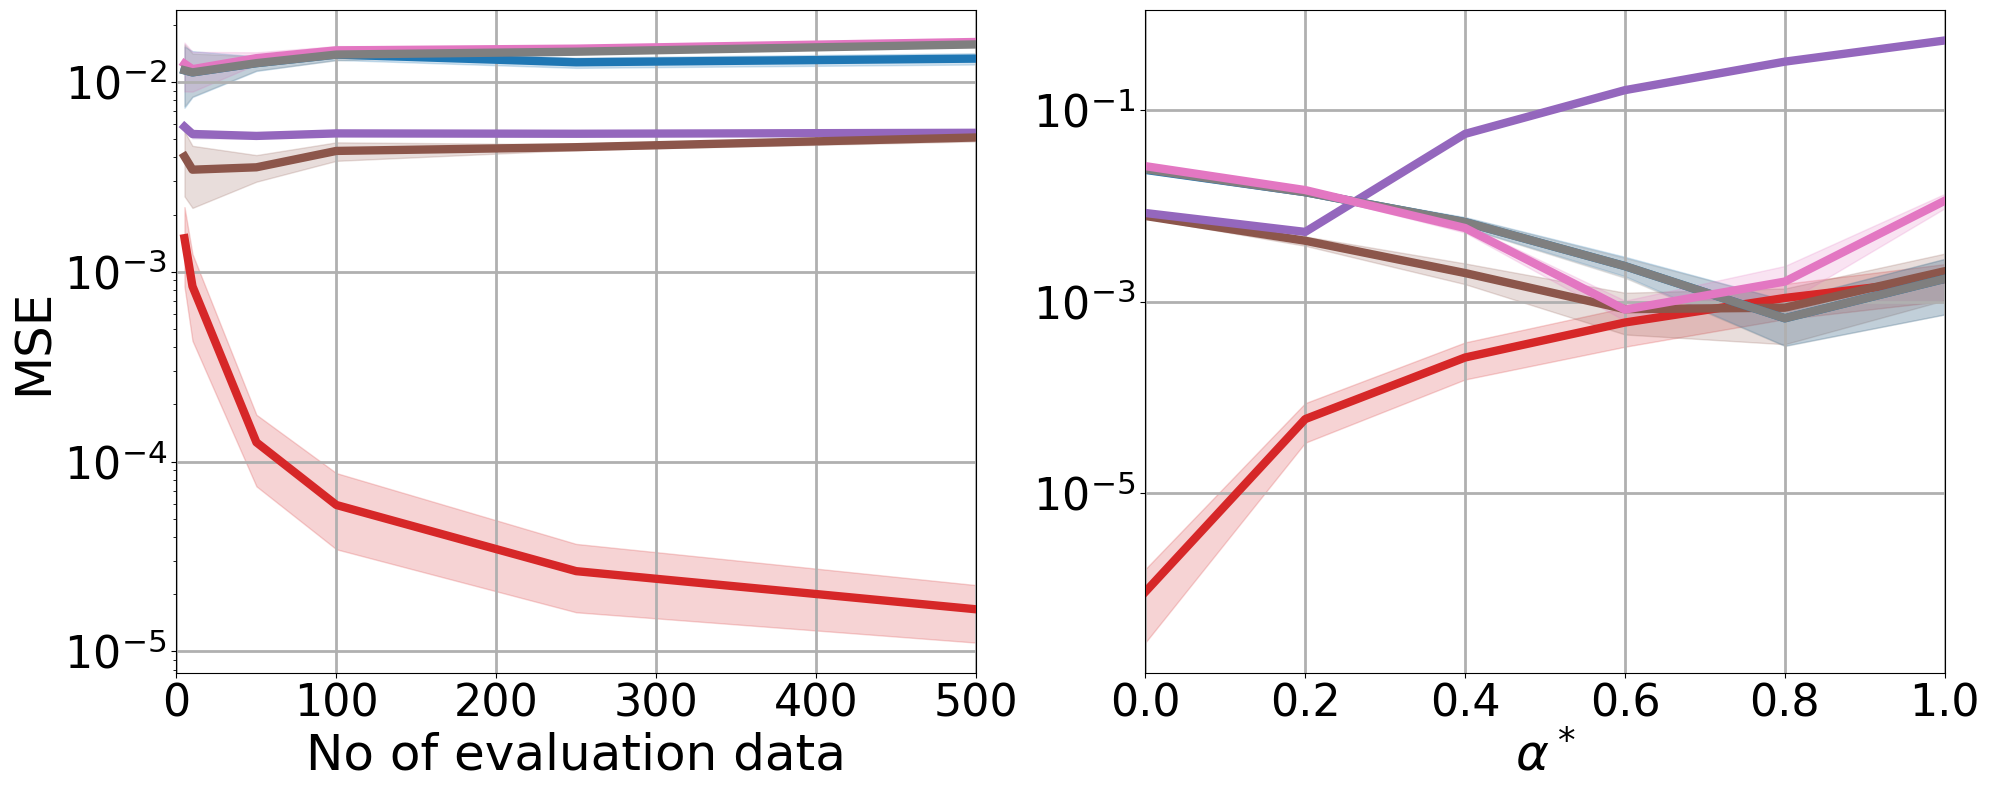
\includegraphics[height=0.92in]{figures/mr/mnist_main.png}
%          \caption{Results for mnist dataset.}
%          \label{fig:mnist-main}
%      \end{subfigure}\\
%     \caption{Results for synthetic data experiment. In \ref{fig:mse-vs-neval} we have $\alpha^\ast=0.8$ and in \ref{fig:mse-vs-betatar} we have $n = 100$.}
%     \label{fig:multiclass-main}
% \end{figure}
% \begin{table}[t]
%     \centering
%     \caption{Mean squared error of target policy value with standard errors over 10 different seeds for different classification datasets. Here, number of evaluation data $n=100$, and $\alpha^\ast=0.2$.}
%     \label{tab:classification-dataset-results}
%     \begin{tiny}
% \begin{tabular}{lllllll}
% \toprule
% Dataset & Digits & Letter & Mnist & OptDigits & PenDigits & SatImage \\
% \midrule
% DM & 0.00505$\pm$0.00016 & 0.01255$\pm$0.00011 & 0.00536$\pm$0.00009 & 0.00240$\pm$0.00009 & 0.00179$\pm$0.00011 & 0.00114$\pm$0.00005 \\
% DR & 0.01768$\pm$0.00058 & 0.00279$\pm$0.00093 & 0.01394$\pm$0.00084 & 0.00590$\pm$0.00089 & 0.00784$\pm$0.00128 & 0.02249$\pm$0.00660 \\
% DRos & 0.01721$\pm$0.00054 & 0.00281$\pm$0.00070 & 0.01467$\pm$0.00068 & 0.00788$\pm$0.00055 & 0.00916$\pm$0.00100 & 0.02160$\pm$0.00237 \\
% IPW & 0.00523$\pm$0.00030 & 0.00142$\pm$0.00062 & 0.00433$\pm$0.00044 & 0.00197$\pm$0.00035 & 0.00367$\pm$0.00077 & 0.01292$\pm$0.00455 \\
% SwitchDR & 0.01768$\pm$0.00058 & 0.00310$\pm$0.00087 & 0.01394$\pm$0.00084 & 0.00709$\pm$0.00054 & 0.00875$\pm$0.00135 & 0.02035$\pm$0.00289 \\
% MR (Ours) & \textbf{0.00011$\pm$0.00002} & \textbf{0.00020$\pm$0.00002} & \textbf{0.00006$\pm$0.00002} & \textbf{0.00025$\pm$0.00009} & \textbf{0.00010$\pm$0.00004} & \textbf{0.00014$\pm$0.00004} \\
% \bottomrule
% \end{tabular}
% \end{tiny}
% \end{table}
% \begin{table}[!htp]
%     \centering
%     \caption{Mean squared error of target policy value with standard errors over 10 different seeds for different classification datasets. Here, number of evaluation data $n=100$, and $\alpha^\ast=0.2$.}
%     \label{tab:classification-dataset-results}
%     \begin{tiny}
% \begin{tabular}{lllllll}
% \toprule
% Dataset & Digits & Letter & OptDigits & PenDigits & SatImage & Mnist \\
% \midrule
% DM & 0.00505$\pm$0.00016 & 0.01255$\pm$0.00011 & 0.00240$\pm$0.00009 & 0.00179$\pm$0.00011 & 0.00114$\pm$0.00005 & 0.00536$\pm$0.00009 \\
% DR & 0.01768$\pm$0.00058 & 0.00279$\pm$0.00093 & 0.00590$\pm$0.00089 & 0.00784$\pm$0.00128 & 0.02249$\pm$0.00660 & 0.01394$\pm$0.00084\\
% DRos & 0.01721$\pm$0.00054 & 0.00281$\pm$0.00070 & 0.00788$\pm$0.00055 & 0.00916$\pm$0.00100 & 0.02160$\pm$0.00237 & 0.01467$\pm$0.00068\\
% IPW & 0.00523$\pm$0.00030 & 0.00142$\pm$0.00062 & 0.00197$\pm$0.00035 & 0.00367$\pm$0.00077 & 0.01292$\pm$0.00455 & 0.00433$\pm$0.00044\\
% SwitchDR & 0.01768$\pm$0.00058 & 0.00310$\pm$0.00087 & 0.00709$\pm$0.00054 & 0.00875$\pm$0.00135 & 0.02035$\pm$0.00289 & 0.01394$\pm$0.00084\\
% MR (Ours) & \textbf{0.00011$\pm$0.00002} & \textbf{0.00020$\pm$0.00002} & \textbf{0.00025$\pm$0.00009} & \textbf{0.00010$\pm$0.00004} & \textbf{0.00014$\pm$0.00004} & \textbf{0.00006$\pm$0.00002}\\
% \bottomrule
% \end{tabular}
% \end{tiny}
% \end{table}
% \vspace{-5mm}
\begin{sidewaystable}[!htp]
    \centering
    \caption{Mean squared error of target policy value with standard errors over 10 different seeds for different classification datasets. Here, number of evaluation data $n=1000$, and $\alpha^\ast=0.6$.}
    \label{tab:classification-dataset-results}
    \begin{footnotesize}
    \begin{scshape}
% \begin{tabular}{lllllll}
% \toprule
% Dataset & Digits & Letter & OptDigits & PenDigits & SatImage & Mnist\\
% \midrule
% DM & 0.16053$\pm$0.00263 & 0.11686$\pm$0.00108 & 0.05963$\pm$0.00129 & 0.05889$\pm$0.00180 & 0.02165$\pm$0.00125 & 0.12556$\pm$0.00112 \\
% DR & 0.05694$\pm$0.00412 & 0.67369$\pm$0.31527 & 0.03697$\pm$0.00707 & 0.20803$\pm$0.13579 & 0.06484$\pm$0.04971 & 0.16665$\pm$0.01689 \\
% DRos & 0.03180$\pm$0.00231 & 0.05629$\pm$0.02057 & 0.00928$\pm$0.00181 & 0.00698$\pm$0.00236 & 0.00824$\pm$0.00212 & 0.06950$\pm$0.00549 \\
% IPW & 0.06465$\pm$0.00459 & 0.96803$\pm$0.44189 & 0.05451$\pm$0.00875 & 0.02769$\pm$0.00720 & 0.02298$\pm$0.00903 & 0.20363$\pm$0.02123 \\
% SwitchDR & 0.05694$\pm$0.00412 & 0.11881$\pm$0.02220 & 0.04086$\pm$0.00711 & 0.02150$\pm$0.00569 & 0.01677$\pm$0.00598 & 0.16665$\pm$0.01689 \\
% MR (Ours) & \textbf{0.00169$\pm$0.00032} & \textbf{0.00126$\pm$0.00045} & \textbf{0.00115$\pm$0.00040} & \textbf{0.00261$\pm$0.00062} & \textbf{0.00314$\pm$0.00071} & \textbf{0.00654$\pm$0.00092} \\
% \bottomrule
% \end{tabular}

\begin{tabular}{llllllll}
\toprule
Dataset &             Digits &               Letter &          OptDigits &          PenDigits &           SatImage  &              Mnist & CIFAR-100\\
\midrule
DM        &  0.1508$\pm$0.0015 &    0.0886$\pm$0.0026 &  0.0485$\pm$0.0016 &   0.0520$\pm$0.0016 &  0.0208$\pm$0.0009  &  0.1109$\pm$0.0014 & 0.0020$\pm$0.0001 \\
DR        &    0.1334$\pm$0.0400 &    \red{35.085$\pm$17.768} &  0.0464$\pm$0.0061 &  0.2343$\pm$0.1404 &   0.0560$\pm$0.0395 &  0.2617$\pm$0.0139 & \red{3823.9$\pm$2023.2} \\
DRos      &  0.0847$\pm$0.0025 &    0.2363$\pm$0.0586 &  0.0384$\pm$0.0025 &  0.0138$\pm$0.0029 &  0.0078$\pm$0.0008 &  0.2151$\pm$0.0061 & 0.2628$\pm$0.1087 \\
IPW       &  0.1632$\pm$0.0462 &  \red{45.253$\pm$22.057} &   0.0844$\pm$0.0056 &  0.1342$\pm$0.0531 &    0.0900$\pm$0.0676 & 0.3359$\pm$0.0118 & \red{4116.9$\pm$2097.9}\\
SwitchDR  &  0.0982$\pm$0.0032 &    0.2387$\pm$0.0507 &  0.0557$\pm$0.0047 &   0.0342$\pm$0.0090 &  0.0136$\pm$0.0012  &   0.2750$\pm$0.0102 & 1.1644$\pm$0.8227 \\
MR (Ours) &  \textbf{0.0034$\pm$0.0001} &    \textbf{0.0018$\pm$0.0004} &  \textbf{0.0006$\pm$0.0002} &  \textbf{0.0008$\pm$0.0002} &  \textbf{0.0016$\pm$0.0003} &  \textbf{0.0121$\pm$0.0009} &  \textbf{0.0007$\pm$0.0002}\\
\bottomrule
\end{tabular}

% \begin{tabular}{lllllll}
% \toprule
% Dataset & Digits & Letter & OptDigits & PenDigits & SatImage & Mnist\\
% \midrule
% DM & 0.161$\pm$0.003 & 0.117$\pm$0.001 & 0.060$\pm$0.001 & 0.059$\pm$0.002 & 0.022$\pm$0.001 & 0.126$\pm$0.001 \\
% DR & 0.057$\pm$0.004 & 0.674$\pm$0.315 & 0.037$\pm$0.007 & 0.208$\pm$0.136 & 0.065$\pm$0.050 & 0.167$\pm$0.017 \\
% DRos & 0.032$\pm$0.002 & 0.056$\pm$0.021 & 0.009$\pm$0.002 & 0.007$\pm$0.002 & 0.008$\pm$0.002 & 0.070$\pm$0.005 \\
% IPW & 0.065$\pm$0.005 & 0.968$\pm$0.442 & 0.055$\pm$0.009 & 0.028$\pm$0.007 & 0.023$\pm$0.009 & 0.204$\pm$0.021 \\
% SwitchDR & 0.057$\pm$0.004 & 0.118$\pm$0.022 & 0.041$\pm$0.007 & 0.022$\pm$0.006 & 0.017$\pm$0.006 & 0.167$\pm$0.017 \\
% MR (Ours) & \textbf{0.002$\pm$0.001} & \textbf{0.001$\pm$0.001} & \textbf{0.001$\pm$0.001} & \textbf{0.003$\pm$0.001} & \textbf{0.003$\pm$0.001} & \textbf{0.007$\pm$0.001} \\
% \bottomrule
% \end{tabular}
\end{scshape}
\end{footnotesize}
\end{sidewaystable}
\subsection{Experiments on classification datasets}
Following previous works on OPE in contextual bandits \citep{dudik2014doubly, kallus2021optimal, mehrdad2018more,wang2017optimal}, we transform classification datasets into contextual bandit feedback data in this experiment.
We consider five UCI classification datasets \citep{dua2019uci} as well as Mnist \citep{deng2012mnist} and CIFAR-100 \citep{krizhevsky2009learning} datasets, each of which comprises $\{(x_i, a^\gt_i)\}_{i}$, where $x_i\in \Xspace$ are feature vectors and $a^\gt_i\in \Aspace$ are the ground-truth labels.
% Here, the datasets considered include five UCI classification datasets \citep{dua2019uci}, as well as the mnist dataset \citep{deng2012mnist}. 
% Following previous works \citep{dudik2014doubly, kallus2021optimal, mehrdad2018more,wang2017optimal}, the classification datasets are transformed to contextual bandit feedback data. 
In the contextual bandits setup, the feature vectors $x_i$ are considered to be the contexts, whereas the actions correspond to the possible class of labels. For the context vector $x_i$ and the action $a_i$, the reward $y_i$ is defined as $y_i \coloneqq \ind(a_i = a^\gt_i)$, i.e., the reward is 1 when the action is the same as the ground truth label and 0 otherwise. Here, the baselines considered include the DM, IPW and DR estimators as well as Switch-DR \citep{wang2017optimal} and DR with Optimistic Shrinkage (DRos) \citep{su2020doubly}. We do not consider a MIPS baseline here as there is no natural embedding $E$ of $A$. Additional details are provided in Appendix \ref{subsec:additional-experiments-classification}. 
% regarding the behaviour and target policies and the estimation of weights are provided in Appendix \ref{sec:app-additional-results}. 
% Similar to the synthetic data experiments, we define a class of parametric target policies parameterised by $\alpha^\ast \in [0, 1]$ (i.e., $\tar = \pi^{\alpha^\ast}$). 
% However, we show in Appendix \ref{subsec:additional-experiments} that in this case, the shift between target and behaviour policies increases as $\alpha^\ast \rightarrow 0$.

In Table \ref{tab:classification-dataset-results}, we present the results with number of evaluation data $n=1000$ and number of training data $m=500$. 
The table shows that across all datasets, MR achieves the lowest MSE among all methods. \flag{Moreover, for the Letter and CIFAR-100 datasets the IPW and DR yield large bias and variance arising from poor policy estimates $\hatbeh$. Despite this, the MR estimator which utilizes the \emph{same} $\hatbeh$ for the estimation of $\hat{w}(y)$ leads to much more accurate results.} We also verify that MR outperforms the baselines for increasing policy shift and evaluation data $n$ in Appendix \ref{subsec:additional-experiments-classification}.
% In fact, the MSE of MR is at least an order of magnitude lower than that of other methods.


% We provide extensive results for increasing policy shift and evaluation data size $n$ in Appendix \ref{sec:app-additional-results}.

% We split the dataset into training and testing datasets of sizes $m$ and $n$ respectively.

% \paragraph{Reward function}
% Let $X$ be a context with ground truth label $A^\gt$, we define the reward for action $A$ as:
% \[
% Y \coloneqq \ind(A = A^\gt).
% \]

\subsection{Application to ATE estimation}\label{subsec:causal-experiments}
% Further to our discussion regarding the application of MR for ATE estimation in Section \ref{subsec:application-to-causal-inference}, 
In this experiment, we investigate the empirical performance of the MR estimator for ATE estimation. 

\myparagraph{Twins dataset}
We use the Twins dataset studied in \cite{louizos2017causal}, which comprises data from twin births in the USA between 1989-1991. The treatment $a=1$ corresponds to being born the heavier twin and the outcome $Y$ corresponds to the mortality of each of the twins in their first year of life. Specifically, $Y(1)$ corresponds to the mortality of the heavier twin (and likewise for $Y(0)$). To simulate the observational study, we follow a similar strategy as in \cite{louizos2017causal} to selectively hide one of the two twins as explained in Appendix \ref{app:ate-empirical}. We obtain a total of 11,984 datapoints, of which 5000 datapoints are used to train the behaviour policy $\hatbeh$ and outcome model $\hat{q}(x, a)$.

% Here, the baselines considered include the DM, IPW and DR estimators as well as Switch-DR \citep{wang2017optimal} and DR with Optimistic Shrinkage (DRos) \citep{su2020doubly}. We do not consider a MIPS baseline here as there is no natural embedding $E$ of $A$. 
% Results for additional baselines have been given in Appendix \ref{app:ate-empirical}. 

% \begin{wraptable}{l}{0.55\textwidth}
\begin{table}[t]
% \vspace{-4mm}
    \centering
    \caption{Mean absolute ATE estimation error $\epsilon_\ate$ with standard errors over 10 different seeds, for increasing number of evaluation data $n$.}
    \label{tab:ate_errors-main}
    \begin{small}
    \begin{tabular}{lllll}
\toprule
$n$ &             50   &             200  &             1600 &             3200 \\
\midrule
DM       &  0.092$\pm$0.003 &  0.092$\pm$0.003 &  0.092$\pm$0.004 &  0.092$\pm$0.004 \\
DR       &  0.101$\pm$0.024 &  \textbf{0.065$\pm$0.009} &  0.071$\pm$0.005 &  0.069$\pm$0.004 \\
\textsc{DRos}     &    0.100$\pm$0.017 &  0.089$\pm$0.006 &   0.093$\pm$0.004 &  0.087$\pm$0.004 \\
IPW      &  0.092$\pm$0.024 &  0.088$\pm$0.014 &  0.067$\pm$0.007 &  0.067$\pm$0.007 \\
\textsc{SwitchDR} &  0.101$\pm$0.024 &  \textbf{0.065$\pm$0.009} &  0.071$\pm$0.005 &  0.069$\pm$0.004 \\
MR (Ours)      &  \textbf{0.062$\pm$0.007} &  \textbf{0.065$\pm$0.007} &  \textbf{0.061$\pm$0.005} &  \textbf{0.061$\pm$0.006} \\
\bottomrule
\end{tabular}
\end{small}
% \vspace{-4mm}
\end{table}
% \end{wraptable}
Here, we consider the same baselines as the classification data experiments in previous section.
For our evaluation, we consider the absolute error in ATE estimation, $\epsilon_\ate$, defined as:
$
\epsilon_\ate \coloneqq | \hat{\theta}^{(n)}_\ate - \theta_\ate |.
$
Here, $\hat{\theta}^{(n)}_\ate$ denotes the value of the ATE estimated using $n$ evaluation datapoints.
%\subsubsection{Results}
We compute the ATE value using the $n$ evaluation datapoints, over 10 different sets of observational data (using different seeds). Table \ref{tab:ate_errors-main} shows that MR achieves the lowest estimation error $\epsilon_\ate$ for all values of $n$ considered here. While the performance of other baselines improves with increasing $n$, MR outperforms them all. 
% Unlike other baselines, MR uses all datapoints to estimate $\E[Y(a)]$ for $a\in \{0, 1\}$ and consequently is more data efficient. 


% \begin{figure}[t]
%      \centering
%      \begin{subfigure}[b]{1\textwidth}
%          \centering
%          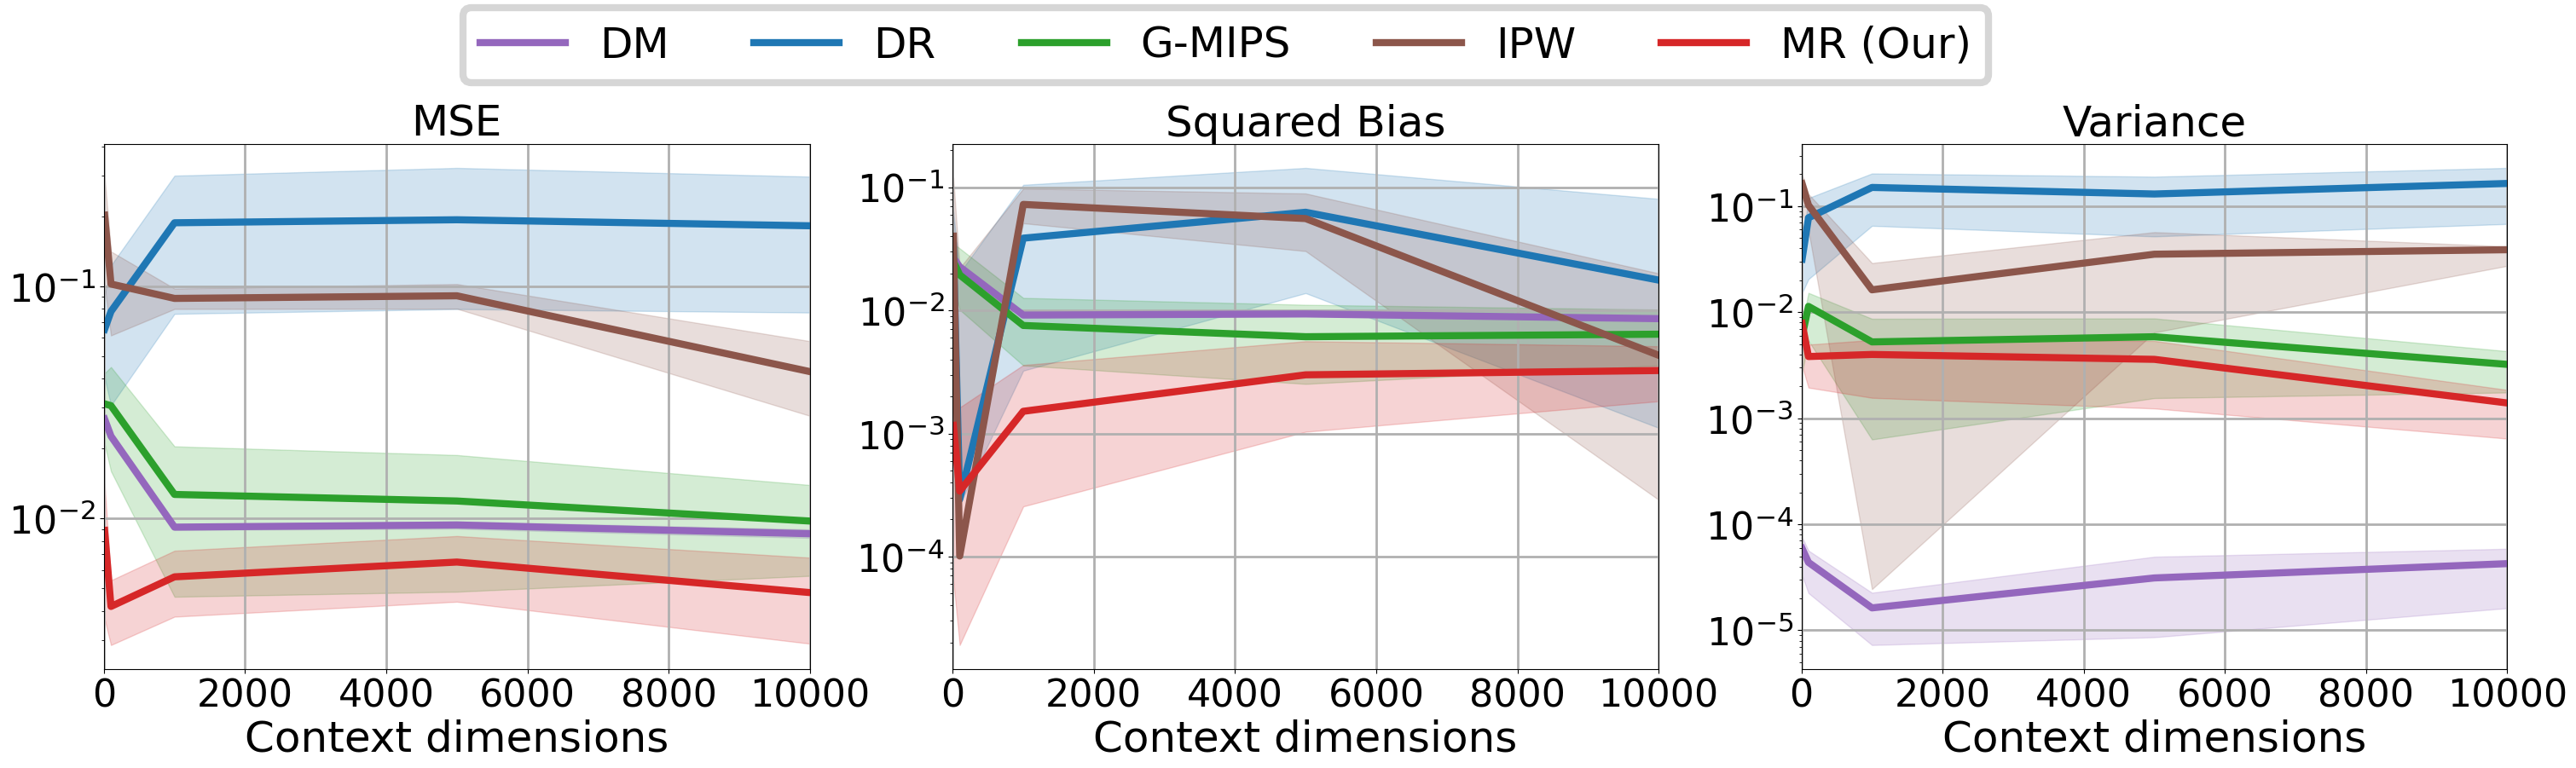
\includegraphics[width=0.75\textwidth]{figures/mr/ope_vs_dimc_nac_100_alphatar_0_8_neval_100_ntrain_100000.png}
%          \caption{Results with varying context dimensions $d$ for $n_{a}=100$, $n = 100$, $\alpha^\ast = 0.8$.}
%          \label{fig:mse-vs-d}
%      \end{subfigure}\\
%      \begin{subfigure}[b]{1\textwidth}
%          \centering
%          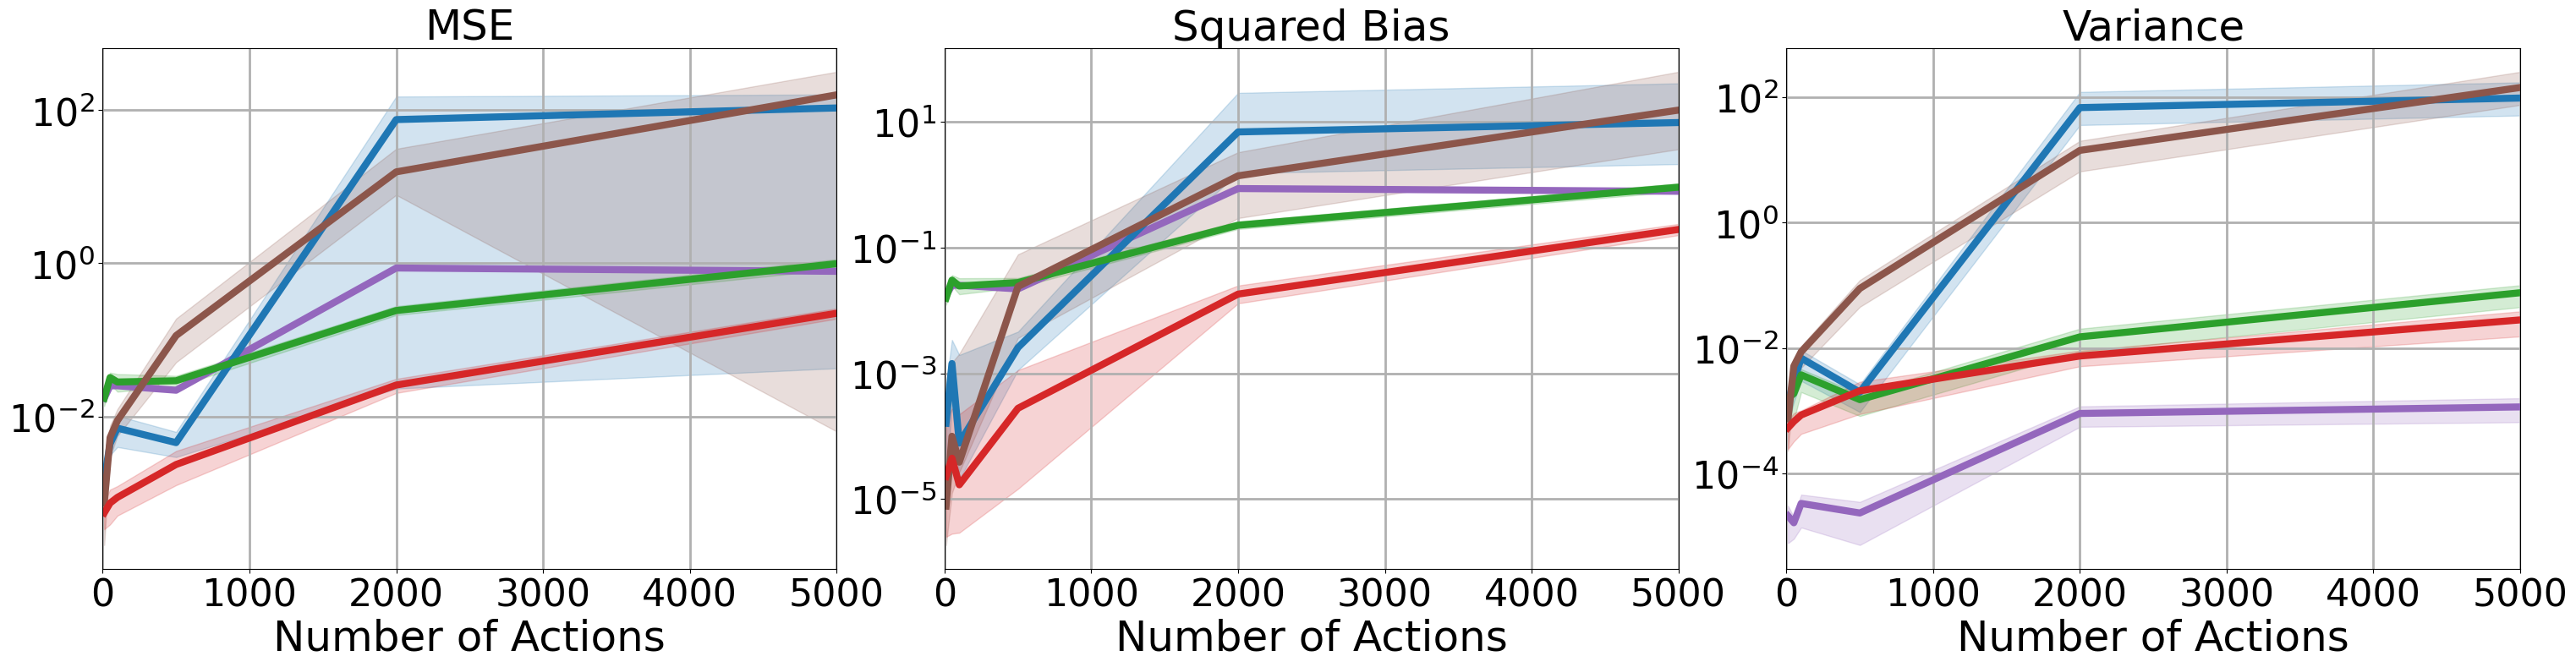
\includegraphics[width=0.75\textwidth]{figures/mr/ope_vs_nac_dimc_100_alphatar_0_2_neval_100_ntrain_100000.png}
%          \caption{Results with varying number of actions $n_{a}$ for $d=100$, $n = 100$, $\alpha^\ast = 0.2$.}
%          \label{fig:mse-vs-nac}
%      \end{subfigure}
%         \caption{Results with increasing $d$ and $n_a$.}
%         \label{fig:syn_results2}
% \end{figure}
% \paragraph{Varying $d$}
% Figure \ref{fig:mse-vs-d} plots how the results for different estimators changes as the context dimensions $d$ increases. While the results for the different baselines do not change significantly with increasing $d$, overall the MSE of MR estimator is smaller than that of other baselines.


% \paragraph{Varying $n_a$}
% Figure \ref{fig:mse-vs-nac} plots how the performance of different estimators changes as the number of actions $n_a$ increases. 
% It can be seen that the MSE and variance of IPW and DR estimators explodes when $n_a \geq 2000$. This happens because the variance of the policy ratios $\rho(a, x)$ is very large for large action spaces. In contrast, the MSE and variances of MR estimator remains relatively small even when $n_a$ is large. This shows that MR remains significantly robust in large action spaces. 

% Again, the MSE of MR estimator remains significantly smaller than the baselines with increasing values of $n_a$.
% \faaiz{think about plotting results versus the variance of policy ratios $\rho(x, a)$.}

\section{Discussion}
% \begin{itemize}
%     \item In this paper, we present marginal ratio estimator (MR) for off-policy evaluation which only considers the shift in the marginal distribution of the rewards resulting from the policy shift.
%     \item We show, theoretically and empirically, that the proposed method achieves better variance and MSE than the current SOTA methods, and is more data efficient overall.
%     \item We also show that our proposal can be used in the setting of causal inference, and provides more accurate results than the most commonly used methods.
% \end{itemize}

In this paper, we proposed an OPE method for contextual bandits called marginal ratio (MR) estimator, which considers only the shift in the marginal distribution of the outcomes resulting from the policy shift. Our theoretical and empirical analysis showed that MR achieves better variance and MSE compared to the current state-of-the-art methods and is more data efficient overall. Additionally, we demonstrated that MR applied to ATE estimation provides more accurate results than most commonly used methods. Next, we discuss limitations of our methodology and possible avenues for future work.

\myparagraph{Limitations}
The MR estimator requires the additional step of estimating $\hat{w}(y)$ which may introduce an additional source of bias in the value estimation. However, $\hat{w}(y)$ can be estimated by solving a simple 1d regression problem, and as we show empirically in Appendix \ref{app:experiments}, MR achieves the smallest bias among all baselines considered in most cases. Most notably, our ablation study in Appendix \ref{subsec:mips-empirical} shows that even when the training data is reasonably small, MR outperforms the baselines considered. 
% When the behaviour policy $\beh$ is unknown, MR estimator requires the splitting of training data to first estimate $\beh$ and subsequently to use this to estimate marginal weights $w(y)$. This data splitting can be costly in low-data settings, where we do not have access to large training datasets. However, as we empirically show in Appendix \ref{subsec:additional-experiments}, even when the training data is small, MR outperforms the baselines.  


\myparagraph{Future work}
The MR estimator can also be applied to policy optimisation problems, where the data collected using an `old' policy is used to learn a new policy. This approach has been used in Proximal Policy Optimisation (PPO) \citep{schulman2017proximal} for example, which has gained immense popularity and has been applied to reinforcement learning with human feedback (RLHF) \citep{lambert2022illustrating}. We believe that the MR estimator applied to these methodologies could lead to improvements in the stability and convergence of these optimisation schemes, given its favourable variance properties.



First and foremost I would like to thank my supervisors Rob Cornish, Arnaud Doucet and Yee Whye Teh 
for their support, patience and invaluable mentorship throughout my DPhil journey. 
They were present for me whenever I needed their help, while also providing me all the flexibility and independence that I needed to conduct my research. 
Their guidance taught me the importance of perseverance, rigour and not compromising on quality -- 
traits which I will cherish for the rest of my life.

I would also like to sincerely thank the collaborators who I have had the privilege of working with throught my DPhil. 
Special thanks to Jean-Francois Ton, Chris Holmes, Lenon Minorics and Yang Liu whose guidance and insights have not only contributed to the success of my research projects but also taught me valuable skills which I will draw upon in future as well.

I am deeply grateful to Google DeepMind for funding my DPhil. 
It would not have been possible for me to pursue my studies without their generous support.

My experience at Oxford would be incomplete without the friendships I developed here. 
I would like to specially mention the amazing people who enriched my time at the department with laughter and camaraderie: 
Jef, Sahra, Emi, Jin, Bobby, Robert, Michael, Alan, Carlo, Andrew, Valentin, Chris, Sheh, Tyler, Jessie, Guneet and Desi.  
Not only did they make my DPhil an enjoyable journey, these are also some of the most smart, talented and supportive individuals that I have ever met and they continue to inspire me everyday. 

To my sister, thank you for being the one unwavering constant in my ever-changing life. 
And to my parents, I cannot express the gratitude I feel for your untiring dedication towards my and my sister's education.
It is impossible for me to list the countless sacrifices that you have made to set us up for success in our lives. 

Finally, I am forever indebted to God for blessing me with this incredible life.
%%%%%%%%%%%%%%%%%%%%%%%%%%%%%%%%%%%%%%%%%%%%%%%%%%%%%%%%%%%%

\bibliography{sample}

\appendix

% \newpage
% \startcontents[sections]
% \printcontents[sections]{l}{1}{\setcounter{tocdepth}{2}}

\newpage

\section{Proofs}
\begin{proof}[Proof of Lemma \ref{lemma:weights-est}]
First, we express the weights $w(y)$ as the conditional expectation as follows:
\begin{align*}
    w(y) &= \frac{\ptar(y)}{\pbeh(y)} \\
    &= \int_{\Xspace, \Aspace} \frac{\ptar(x,a,y)}{\pbeh(y)}\,\mathrm{d}a\, \mathrm{d}x\\
    &= \int_{\Xspace, \Aspace} \frac{\ptar(x,a,y)}{\pbeh(y)}\,\frac{\pbeh(x, a\mid y)}{\pbeh(x, a\mid y)}\,\mathrm{d}a\, \mathrm{d}x\\
    &= \int_{\Xspace, \Aspace} \frac{\ptar(x,a,y)}{\pbeh(x, a, y)}\,\pbeh(x, a\mid y)\,\mathrm{d}a\, \mathrm{d}x\\
    &= \int_{\Xspace, \Aspace} \rho(a, x)\,\pbeh(x, a\mid y)\,\mathrm{d}a\, \mathrm{d}x\\
    &= \Ebeh[\rho(A, X)\mid Y=y],
\end{align*}
where $\rho(a, x) = \frac{\ptar(x, a, y)}{\pbeh(x, a, y)} = \frac{\tar(a\mid x)}{\beh(a\mid x)}$.
Since conditional expectations can be defined as the solution of regression problem, the result follows. 
\end{proof}

\begin{proof}[Proof of Proposition \ref{tv_prop}] We have
\begin{align*}
    \textup{D}_f\left(\ptar(x,a,y)\,||\, \pbeh(x,a,y)\right) &= \Ebeh\left[ f\left( \frac{\ptar(X,A,Y)}{\pbeh(X,A,Y)}\right) \right]\\
    &= \Ebeh\left[ f\left( \frac{\tar(A\mid X)}{\beh(A\mid X)}\right) \right]\\
    &= \Ebeh\left[\Ebeh\left[ f\left( \frac{\tar(A\mid X)}{\beh(A\mid X)}\right) \Bigg| Y \right]\right]\\
    &\geq \Ebeh\left[ f\left( \Ebeh\left[\frac{\tar(A\mid X)}{\beh(A\mid X)}\Bigg| Y \right]\right) \right]\quad\text{(Jensen's inequality)}\\
    &= \Ebeh\left[ f\left( \frac{\ptar(Y)}{\pbeh(Y)} \right) \right]\\
    &= \textup{D}_f\left(\ptar(y)\,||\, \pbeh(y)\right).
\end{align*}
\end{proof}

\begin{proof}[Proof of Proposition \ref{prop:var_mr}]
Since $\Ebeh[\thetaipw] = \Ebeh[\thetamr] = \Etar[Y]$, we have that,  
\begin{align*}
    \Vbeh[\thetaipw] - \Vbeh[\thetamr] &= \Ebeh[\thetaipw]^2 - \Ebeh[\thetamr]^2 \\
    &= \frac{1}{n} \left(\Ebeh\left[\rho(A, X)^2\, Y^2 \right] - \Ebeh\left[w(Y)^2\, Y^2 \right] \right)\\
    &= \frac{1}{n} \left(\Ebeh\left[\Ebeh[\rho(A, X)^2\mid Y]\, Y^2 \right] - \Ebeh\left[w(Y)^2\, Y^2 \right] \right)\\
    &= \frac{1}{n} \left(\Ebeh\left[\Ebeh[\rho(A, X)^2\mid Y]\, Y^2 \right] - \Ebeh\left[\Ebeh[\rho(A, X)\mid Y]^2\, Y^2 \right] \right)\\
    &= \frac{1}{n} \Ebeh \left[ \Vbeh\left[ \rho(A, X) \mid Y \right]\, Y^2 \right].
\end{align*}
In the second last step above, we use the fact that $w(y) = \Ebeh[\rho(A, X)\mid Y=y]$. 
\end{proof}

\begin{proof}[Proof of Proposition \ref{prop:var_dr}]
Let $\hat{\mu}(a, x) \approx \E[Y\mid X=x, A=a]$ denote the outcome model in DR estimator. Then, using multiple applications of the law of total variance we get that
\begin{align*}
    n\, \Vbeh[\thetadr] &= \Vbeh\left[\rho(A, X)\,(Y - \hat{\mu}(A, X)) + \sum_{a'\in \Aspace} \hat{\mu}(a', X)\,\tar(a'\mid X)\right]\\
    &= \Vbeh\left[\rho(A, X)\,(Y - \hat{\mu}(A, X)) + \Etar[\hat{\mu}(A, X)\mid X]\right]\\
    &= \Ebeh[\Vbeh[\rho(A, X)\,(Y - \hat{\mu}(A, X)) + \Etar[\hat{\mu}(A, X)\mid X]\mid X, A]]\\
    &\quad+ \Vbeh[\Ebeh[\rho(A, X)\,(Y - \hat{\mu}(A, X)) + \Etar[\hat{\mu}(A, X)\mid X]\mid X, A]]\\
    &= \Ebeh[\rho(A, X)^2 \var[Y\mid X, A]] \\
    &\quad+ \Vbeh[\Ebeh[\rho(A, X)\,(Y - \hat{\mu}(A, X)) + \Ebeh[\rho(A, X)\,\hat{\mu}(A, X)\mid X]\mid X, A]]\\
    &= \Ebeh[\rho(A, X)^2 \var[Y\mid X, A]] \\
    &\quad+ \Vbeh[\rho(A, X)\,(\mu(A, X) - \hat{\mu}(A, X)) + \Ebeh[\rho(A, X)\,\hat{\mu}(A, X)\mid X]]\\
    &= \Ebeh[\rho(A, X)^2 \var[Y\mid X, A]] \\
    &\quad+ \Vbeh[\Ebeh[\rho(A, X)\,(\mu(A, X) - \hat{\mu}(A, X)) + \Ebeh[\rho(A, X)\,\hat{\mu}(A, X)\mid X]\mid X]] \\
    &\quad+ \Ebeh[\Vbeh[\rho(A, X)\,(\mu(A, X) - \hat{\mu}(A, X)) + \Ebeh[\rho(A, X)\,\hat{\mu}(A, X)\mid X]\mid X]]\\
    &= \Ebeh[\rho(A, X)^2 \var[Y\mid X, A]]+ \Vbeh[\Ebeh[\rho(A, X)\,\mu(A, X)\mid X]] \\
    &\quad+ \Ebeh[\Vbeh[\rho(A, X)\,(\mu(A, X) - \hat{\mu}(A, X))\mid X]]\\
    &\geq \Ebeh[\rho(A, X)^2 \var[Y\mid X, A]] + \Vbeh[\Ebeh[\rho(A, X)\,\mu(A, X)\mid X]].
\end{align*}
Using this, we get that
\begin{align*}
    &n (\Vbeh[\thetadr] - \Vbeh[\thetamr]) \\
    &\quad\geq \Ebeh[\rho(A, X)^2 \var[Y\mid X, A]] +  \Vbeh \left[\Ebeh[\rho(A, X) \,\mu(A, X)\mid X]\right] - \Vbeh[w(Y)\,Y].
\end{align*}
Again, using the law of total variance,
\begin{align*}
    \Vbeh[\rho(A, X)\,Y] &= \Ebeh[\Vbeh[\rho(A, X)\,Y \mid X, A]] + \Vbeh[\Ebeh[\rho(A, X)\,Y\mid X, A]]\\
    &= \Ebeh[\rho(A, X)^2\var[Y \mid X, A]] + \Vbeh[ \rho(A, X)\,\mu(A, X)]\\
    &= \Ebeh[\rho(A, X)^2\var[Y \mid X, A]] + \Vbeh \left[\Ebeh[\rho(A, X) \,\mu(A, X)\mid X]\right] \\
    &\quad+ \Ebeh \left[\Vbeh[\rho(A, X) \,\mu(A, X)\mid X]\right].
\end{align*}
Rearranging and substituting back into the expression earlier, we get that
\begin{align*}
    &n (\Vbeh[\thetadr] - \Vbeh[\thetamr]) \\
    &\quad\geq \Vbeh[\rho(A, X)\,Y] - \Ebeh \left[\Vbeh[\rho(A, X) \,\mu(A, X)\mid X]\right] - \Vbeh[w(Y)\,Y].
\end{align*}
Now, from Proposition \ref{prop:var_mr} we know that \begin{align*}
    n (\Vbeh[\thetaipw] - \Vbeh[\thetamr]) = \Vbeh[\rho(A, X)\,Y] - \Vbeh[w(Y)\,Y] = \Ebeh \left[ \Vbeh\left[ \rho(A, X) \mid Y \right]\, Y^2 \right].
\end{align*}
Therefore, 
\begin{align*}
    &n (\Vbeh[\thetadr] - \Vbeh[\thetamr]) \\
    &\quad\geq \Ebeh \left[ \Vbeh\left[ \rho(A, X) \mid Y \right]\, Y^2 \right] - \Ebeh \left[\Vbeh[\rho(A, X) \,\mu(A, X)\mid X]\right]\\
    &\quad= \Ebeh \left[\Vbeh\left[ \rho(A, X)\,Y \mid Y \right] - \Vbeh[\rho(A, X) \,\mu(A, X)\mid X] \right].
\end{align*}
\end{proof}

% \begin{proof}[Proof of Proposition \ref{prop:var_dr}]
% Let $\hat{\mu}(a, x) \approx \E[Y\mid x, a]$ denote the outcome model in DR estimator. From \cite[Lemma 3.3(i)]{dudik2014doubly}, we know that
% \begin{align*}
%     n\, \Vbeh[\thetadr] &= \Ebeh[\rho(A, X)^2 \var[Y\mid X, A]] +  \var_{X\sim p(X)} \left[\Ebeh[\rho(A, X) \,\mu(A, X)\mid X]\right] \\
%     &\quad+ \E_{X\sim p(X)}[\Vbeh[\rho(A, X)(\hat{\mu}(A, X) - \mu(A, X))]]\\
%     &\geq \Ebeh[\rho(A, X)^2 \var[Y\mid X, A]] +  \var_{X\sim p(X)} \left[\Ebeh[\rho(A, X) \,\mu(A, X)\mid X]\right].
% \end{align*}
% Using this, we get that
% \begin{align*}
%     &n (\Vbeh[\thetadr] - \Vbeh[\thetamr]) \\
%     &\quad\geq \Ebeh[\rho(A, X)^2 \var[Y\mid X, A]] +  \var_{X\sim p(X)} \left[\Ebeh[\rho(A, X) \,\mu(A, X)\mid X]\right] - \Vbeh[w(Y)\,Y].
% \end{align*}
% Now, using the law of total variance,
% \begin{align*}
%     \Vbeh[\rho(A, X)\,Y] &= \Ebeh[\Vbeh[\rho(A, X)\,Y \mid X, A]] + \Vbeh[\Ebeh[\rho(A, X)\,Y\mid X, A]]\\
%     &= \Ebeh[\rho(A, X)^2\var[Y \mid X, A]] + \Vbeh[ \rho(A, X)\,\mu(A, X)]\\
%     &= \Ebeh[\rho(A, X)^2\var[Y \mid X, A]] + \var_{X\sim p(X)} \left[\Ebeh[\rho(A, X) \,\mu(A, X)\mid X]\right] \\
%     &\quad+ \E_{X\sim p(X)} \left[\Vbeh[\rho(A, X) \,\mu(A, X)\mid X]\right].
% \end{align*}
% Rearranging and substituting back into the expression earlier, we get that
% \begin{align*}
%     &n (\Vbeh[\thetadr] - \Vbeh[\thetamr]) \\
%     &\quad\geq \Vbeh[\rho(A, X)\,Y] - \E_{X\sim p(X)} \left[\Vbeh[\rho(A, X) \,\mu(A, X)\mid X]\right] - \Vbeh[w(Y)\,Y].
% \end{align*}
% Now, from Proposition \ref{prop:var_mr} we know that \begin{align*}
%     n (\Vbeh[\thetaipw] - \Vbeh[\thetamr]) = \Vbeh[\rho(A, X)\,Y] - \Vbeh[w(Y)\,Y] = \E_{Y\sim \pbeh(Y)} \left[ \Vbeh\left[ \rho(A, X) \mid Y \right]\, Y^2 \right].
% \end{align*}
% Therefore, 
% \begin{align*}
%     &n (\Vbeh[\thetadr] - \Vbeh[\thetamr]) \\
%     &\quad\geq \E_{Y\sim \pbeh(Y)} \left[ \Vbeh\left[ \rho(A, X) \mid Y \right]\, Y^2 \right] - \E_{X\sim p(X)} \left[\Vbeh[\rho(A, X) \,\mu(A, X)\mid X]\right]\\
%     &\quad= \Ebeh \left[\Vbeh\left[ \rho(A, X) \mid Y \right]\, Y^2 - \Vbeh[\rho(A, X) \,\mu(A, X)\mid X] \right].
% \end{align*}
% \end{proof}

\begin{comment}
    

\begin{proof}[Proof of Proposition \ref{prop:mips_var_reduction}]
The following proof, which is included for completeness, is a straightforward extension of \cite[Theorem 3.6]{saito2022off}. 
\begin{align*}
    &n (\Vbeh[\thetaipw] - \Vbeh[\hat{\theta}_{\textup{MIPS}}])\\
    &\quad= \Vbeh\left[\frac{\tar(A|X)}{\beh(A|X)}\,Y\right] - \Vbeh\left[\frac{\ptar(R)}{\pbeh(R)}\,Y \right]\\
     &\quad= \Vbeh\left[\Ebeh\left[\frac{\tar(A|X)}{\beh(A|X)}\,Y \Bigg| R\right]\right] + \Ebeh\left[ \Vbeh\left[\frac{\tar(A|X)}{\beh(A|X)}\,Y\Bigg| R \right]\right] - \Vbeh\left[\Ebeh\left[ \frac{\ptar(R)}{\pbeh(R)}\,Y \Bigg| R\right]\right]\\
     &\qquad- \Ebeh\left[\Vbeh\left[ \frac{\ptar(R)}{\pbeh(R)}\,Y \Bigg| R\right]\right]
\end{align*}
Now using the conditional independence Assumption \ref{assum:indep-general}, the first term on the RHS above becomes,
\begin{align*}
    \Vbeh\left[\Ebeh\left[\frac{\tar(A|X)}{\beh(A|X)}\,Y \Bigg| R\right]\right] &= \Vbeh\left[\Ebeh\left[\frac{\tar(A|X)}{\beh(A|X)}\Bigg| R\right]\,\Ebeh\left[Y | R\right]\right]\\
    &= \Vbeh\left[\frac{\ptar(R)}{\pbeh(R)}\,\Ebeh\left[Y | R\right]\right],
\end{align*}
where in the last step above we use the fact that
\begin{align*}
    \Ebeh\left[\frac{\tar(A|X)}{\beh(A|X)}\Bigg| R\right] = \frac{\ptar(R)}{\pbeh(R)}.
\end{align*}
Putting this together, we get that
\begin{align}
    &n (\Vbeh[\thetaipw] - \Vbeh[\hat{\theta}_{\textup{MIPS}}]) \nonumber\\ 
    &\quad= \Ebeh\left[ \Vbeh\left[\frac{\tar(A|X)}{\beh(A|X)}\,Y\Bigg| R \right]\right] - \Ebeh\left[\Vbeh\left[ \frac{\ptar(R)}{\pbeh(R)}\,Y \Bigg| R\right]\right]. \label{eq:variance-difference}
\end{align}
Since we have that 
\begin{align*}
    \Ebeh\left[\frac{\tar(A|X)}{\beh(A|X)}\,Y\Bigg| R \right] = \Ebeh\left[\frac{\tar(A|X)}{\beh(A|X)}\Bigg| R \right]\,\Ebeh\left[Y| R \right] = \frac{\ptar(R)}{\pbeh(R)}\,\Ebeh\left[Y| R \right],
\end{align*}
Eq. \eqref{eq:variance-difference} becomes,
\begin{align*}
    &\Ebeh\left[ \Vbeh\left[\frac{\tar(A|X)}{\beh(A|X)}\,Y\Bigg| R \right]\right] - \Ebeh\left[\Vbeh\left[ \frac{\ptar(R)}{\pbeh(R)}\,Y \Bigg| R\right]\right] \\
    &\quad= \Ebeh\left[ \Ebeh\left[ \left(\frac{\tar(A|X)}{\beh(A|X)}\,Y \right)^2\Bigg| R  \right] - \Ebeh\left[ \left(\frac{\ptar(R)}{\pbeh(R)}\,Y \right)^2\Bigg| R \right] \right]\\
    &\quad= \Ebeh\left[ \Ebeh\left[ \left(\frac{\tar(A|X)}{\beh(A|X)} \right)^2 \Bigg| R  \right] \, \Ebeh\left[Y^2 | R  \right] - \left(\frac{\ptar(R)}{\pbeh(R)}\right)^2\,\Ebeh\left[Y^2 | R \right] \right]\\
    &\quad= \Ebeh\left[\Ebeh\left[Y^2 | R \right]\, \left( \Ebeh\left[ \left(\frac{\tar(A|X)}{\beh(A|X)} \right)^2 \Bigg| R  \right] - \left(\Ebeh\left[ \frac{\tar(A|X)}{\beh(A|X)} \Bigg| R  \right]\right)^2\, \right) \right]\\
    &\quad=\Ebeh\left[\Ebeh\left[Y^2 | R \right]\, \Vbeh\left[\frac{\tar(A|X)}{\beh(A|X)} \Bigg| R \right]\right].
\end{align*}
\end{proof}
\end{comment}
\begin{comment}

\begin{proof}[Proof of Proposition \ref{prop:bias-and-var}]
\begin{align*}
    \textup{Bias}(\thetaipw) &= \Ebeh[\hat{\rho}(A, X)\, Y] - \Etar[Y] \\
    &= \Ebeh\left[\Ebeh[\hat{\rho}(A, X)\mid Y]\,Y \right] - \Etar[Y]  \\
    &= \Ebeh[\hat{w}(Y)\, Y] - \Etar[Y] \\
    &= \textup{Bias}(\thetadr)
\end{align*}
Next, we prove the variance result.
As shown above, $\Ebeh[\thetaipw] = \Ebeh[\thetamr]$. Therefore, we have that,  
\begin{align*}
    \Vbeh[\thetaipw] - \Vbeh[\thetamr] &= \Ebeh[\thetaipw]^2 - \Ebeh[\thetamr]^2 \\
    &= \frac{1}{n} \left(\Ebeh\left[\hat{\rho}(A, X)^2\, Y^2 \right] - \Ebeh\left[\hat{w}(Y)^2\, Y^2 \right] \right)\\
    &= \frac{1}{n} \left(\E_{Y\sim\pbeh(Y)}\left[\Ebeh[\hat{\rho}(A, X)^2\mid Y]\, Y^2 \right] - \Ebeh\left[\hat{w}(Y)^2\, Y^2 \right] \right)\\
    &= \frac{1}{n} \left(\E_{Y\sim\pbeh(Y)}\left[\Ebeh[\hat{\rho}(A, X)^2\mid Y]\, Y^2 \right] - \E_{Y\sim\pbeh(Y)}\left[\Ebeh[\hat{\rho}(A, X)\mid Y]^2\, Y^2 \right] \right)\\
    &= \frac{1}{n} \E_{Y\sim \pbeh(Y)} \left[ \Vbeh\left[ \hat{\rho}(A, X) \mid Y \right]\, Y^2 \right].
\end{align*}
Where, in the second last step above we use the fact that almost surely, $\hat{w}(Y) = \Ebeh[\hat{\rho}(A, X)\mid Y]$.
\end{proof}
\end{comment}


% \begin{proof}[Proof of Proposition \ref{prop:mips_generalised}]
%     First, we prove that the MIPS estimators are unbiased using induction on $j$. When $j=0$, we recover the IPW estimator, which we know is unbiased. Now, assume that $\Ebeh[\hat{\theta}^{(j)}_{\textup{MIPS}}] = \Etar[Y]$.

%     Conditional on $R^{(j)}$, $R^{(j+1)}$ does not depend on the policy. Therefore, 
%     \begin{align*}
%         \frac{\ptar(r^{(j)})}{\pbeh(r^{(j)})} = \frac{\ptar(r^{(j)})\,p(r^{(j+1)}\mid r^{(j)}) }{\pbeh(r^{(j)})\,p(r^{(j+1)}\mid r^{(j)})} = \frac{\ptar(r^{(j)}, r^{(j+1)})}{\pbeh(r^{(j)}, r^{(j+1)})}.
%     \end{align*}
%     And therefore,
%     \begin{align*}
%         \frac{\ptar(r^{(j+1)})}{\pbeh(r^{(j+1)})} &= \int_{r^{(j)}} \frac{\ptar(r^{(j)}, r^{(j+1)})}{\pbeh(r^{(j)}, r^{(j+1)})} \, \pbeh(r^{(j)} \mid r^{(j+1)}) \,\mathrm{d} r^{(j)}\\ 
%         &= \int_{r^{(j)}} \frac{\ptar(r^{(j)})}{\pbeh(r^{(j)})} \,\pbeh(r^{(j)} \mid r^{(j+1)}) \,\mathrm{d} r^{(j)}\\ 
%         &= \Ebeh\left[\frac{\ptar(R^{(j)})}{\pbeh(R^{(j)})} \Bigg|  R^{(j+1)}=r^{(j+1)}\right].
%     \end{align*}
%     Using this and the fact that $R^{(j)}\indep Y \mid R^{(j+1)}$, we get that
%     \begin{align*}
%         \Ebeh\left[\hat{\theta}^{(j+1)}_{\textup{MIPS}} \right] &= \Ebeh\left[\frac{\ptar(R^{(j+1)})}{\pbeh(R^{(j+1)})}\, Y \right]\\
%         &= \Ebeh\left[\frac{\ptar(R^{(j+1)})}{\pbeh(R^{(j+1)})}\, \Ebeh[Y| R^{(j+1)}] \right]\\
%         &= \Ebeh\left[\Ebeh\left[\frac{\ptar(R^{(j)})}{\pbeh(R^{(j)})} \Bigg|  R^{(j+1)}\right]\, \Ebeh[Y| R^{(j+1)}] \right] \\
%         &= \Ebeh\left[\Ebeh\left[\frac{\ptar(R^{(j)})}{\pbeh(R^{(j)})} \, Y \Bigg|  R^{(j+1)}\right]\right]\\
%         &= \Ebeh\left[ \frac{\ptar(R^{(j)})}{\pbeh(R^{(j)})} \, Y \right]\\
%         &= \Ebeh\left[\hat{\theta}^{(j)}_{\textup{MIPS}} \right] = \Etar[Y].
%     \end{align*}
%     Next, to prove the variance result we consider the difference
%     \begin{align*}
%         &\Vbeh[\hat{\theta}^{(j)}_{\textup{MIPS}}] - \Vbeh[\hat{\theta}^{(j+1)}_{\textup{MIPS}}] \\
%         &= \frac{1}{n}\left(\Vbeh\left[\frac{\ptar(R^{(j)})}{\pbeh(R^{(j)})}\, Y\right] - \Vbeh\left[\frac{\ptar(R^{(j+1)})}{\pbeh(R^{(j+1)})}\, Y\right]\right) \\
%         % &= \frac{1}{n}\left(\Vbeh\left[\frac{\ptar(R^{(j)})}{\pbeh(R^{(j)})}\, Y\right] - \Vbeh\left[\Ebeh\left[\frac{\ptar(R^{(j)})}{\pbeh(R^{(j)})} \Bigg|  R^{(j+1)}\right]\, Y\right]\right)\\
%         &= \frac{1}{n}\Bigg(\Vbeh\left[ \Ebeh\left[\frac{\ptar(R^{(j)})}{\pbeh(R^{(j)})}\, Y \Bigg| R^{(j+1)} \right] \right] + \Ebeh\left[ \Vbeh\left[\frac{\ptar(R^{(j)})}{\pbeh(R^{(j)})}\, Y \Bigg| R^{(j+1)} \right] \right] \\
%         &\qquad- \Vbeh\left[\frac{\ptar(R^{(j+1)})}{\pbeh(R^{(j+1)})}\, \Ebeh[Y\mid R^{(j+1)}]\right] - \Ebeh \left[\left(\frac{\ptar(R^{(j+1)})}{\pbeh(R^{(j+1)})}\right)^2\,\Vbeh[Y\mid R^{(j+1)}] \right] \Bigg)
%     \end{align*}
%     where in the last step we use the law of total variance. Now, using the fact that $R^{(j)}\indep Y \mid R^{(j+1)}$, we can rewrite the expression above as
%     \begin{align*}
%         &= \frac{1}{n}\Bigg(\Vbeh\left[ \Ebeh\left[\frac{\ptar(R^{(j)})}{\pbeh(R^{(j)})}\Bigg| R^{(j+1)} \right]\, \Ebeh[Y | R^{(j+1)} ] \right] + \Ebeh\left[ \Vbeh\left[\frac{\ptar(R^{(j)})}{\pbeh(R^{(j)})}\, Y \Bigg| R^{(j+1)} \right] \right] \\
%         &\qquad- \Vbeh\left[\frac{\ptar(R^{(j+1)})}{\pbeh(R^{(j+1)})}\, \Ebeh[Y\mid R^{(j+1)}]\right] - \Ebeh \left[\left(\frac{\ptar(R^{(j+1)})}{\pbeh(R^{(j+1)})}\right)^2\,\Vbeh[Y\mid R^{(j+1)}] \right] \Bigg)\\
%         &= \frac{1}{n}\Bigg( \Ebeh\left[ \Vbeh\left[\frac{\ptar(R^{(j)})}{\pbeh(R^{(j)})}\, Y \Bigg| R^{(j+1)} \right] \right] - \Ebeh \left[\left(\frac{\ptar(R^{(j+1)})}{\pbeh(R^{(j+1)})}\right)^2\,\Vbeh[Y\mid R^{(j+1)}] \right]\Bigg)
%     \end{align*}
%     Moreover, again using the conditional independence $R^{(j)}\indep Y \mid R^{(j+1)}$, we can expand the first term in the expression above as follows:
%     % \begin{align*}
%     %     \Vbeh\left[ \Ebeh\left[\frac{\ptar(R^{(j)})}{\pbeh(R^{(j)})}\, Y \Bigg| R^{(j+1)} \right] \right] &=
%     %     \Vbeh\left[ \Ebeh\left[\frac{\ptar(R^{(j)})}{\pbeh(R^{(j)})}\Bigg| R^{(j+1)}\right]\, \Ebeh\left[Y | R^{(j+1)} \right] \right]\\
%     %     &= \Vbeh\left[ \frac{\ptar(R^{(j+1)})}{\pbeh(R^{(j+1)})}\, \Ebeh\left[Y | R^{(j+1)} \right]\right]
%     % \end{align*}
%     \begin{align*}
%         \Ebeh\left[ \Vbeh\left[\frac{\ptar(R^{(j)})}{\pbeh(R^{(j)})}\, Y \Bigg| R^{(j+1)} \right] \right] &=
%         \Ebeh\Bigg[ \Ebeh\left[\frac{\ptar^2(R^{(j)})}{\pbeh^2(R^{(j)})} \Bigg| R^{(j+1)} \right]\,\Ebeh[Y^2 | R^{(j+1)}] \\
%         &\qquad- \left(\Ebeh\left[\frac{\ptar(R^{(j)})}{\pbeh(R^{(j)})} \Bigg| R^{(j+1)} \right] \Ebeh[Y | R^{(j+1)}] \right)^2 \Bigg]\\
%         &\geq 
%         \Ebeh\Bigg[ \left(\Ebeh\left[\frac{\ptar(R^{(j)})}{\pbeh(R^{(j)})} \Bigg| R^{(j+1)} \right]\right)^2 \,\Ebeh[Y^2 | R^{(j+1)}] \\
%         &\qquad- \left(\frac{\ptar(R^{(j+1)})}{\pbeh(R^{(j+1)})} \Ebeh[Y | R^{(j+1)}] \right)^2 \Bigg]\\
%         &= \Ebeh\Bigg[ \left(\frac{\ptar(R^{(j+1)})}{\pbeh(R^{(j+1)})}\right)^2 \, \Vbeh[Y\mid R^{(j+1)}] \Bigg]
%     \end{align*}
%     Here, to get the inequality above, we use the fact that $\E[X^2] \geq (\E[X])^2$. Putting this together, we get that $\Vbeh[\hat{\theta}^{(j)}_{\textup{MIPS}}] - \Vbeh[\hat{\theta}^{(j+1)}_{\textup{MIPS}}] \geq 0$.

%     Moreover, the result $\Vbeh[\hat{\theta}^{(2)}_{\textup{MIPS}}] \geq \Vbeh[\thetamr]$ follows straightforwardly from above by defining $R^{(3)} \coloneqq Y$. Then, the embeddings satisfy the causal structure 
%     \[
%     R^{(0)} \rightarrow R^{(1)} \rightarrow R^{(2)}  \rightarrow R^{(3)} \rightarrow Y.
%     \]
%     Using the result above, we know that $\Vbeh[\hat{\theta}^{(2)}_{\textup{MIPS}}] \geq \Vbeh[\hat{\theta}^{(3)}_{\textup{MIPS}}]$. But now it is straightforward to see that $\hat{\theta}^{(3)}_{\textup{MIPS}} = \thetamr$, and the result follows.
% \end{proof}

\begin{proof}[Proof of Theorem \ref{prop:mips_main_text}]
This result follows straightforwardly from Proposition \ref{prop:mips_generalised} in Appendix \ref{app:gmips}.    
\end{proof}

\begin{proof}[Proof of Proposition \ref{prop:bias-and-var-main}]
\begin{align*}
    \textup{Bias}(\thetaipw) &= \Ebeh[\hat{\rho}(A, X)\, Y] - \Etar[Y] \\
    &= \Ebeh\left[\Ebeh[\hat{\rho}(A, X)\mid Y]\,Y \right] - \Etar[Y]  \\
    &= \Ebeh[\hat{w}(Y)\, Y] - \Ebeh[\epsilon\, Y] - \Etar[Y] \\
    % &= \Ebeh[\hat{w}(Y)\, Y] - \Etar[Y]\\
    &= \textup{Bias}(\thetamr) - \Ebeh[\epsilon\, Y].
\end{align*}
Next, to prove the variance result, we first use the law of total variance to obtain
\begin{align*}
    \Vbeh[\thetaipw] &= \frac{1}{n} \Vbeh[\hat{\rho}(A, X)\,Y]\\
    &= \frac{1}{n} \left( \Vbeh[\Ebeh[\hat{\rho}(A, X)\,Y\mid Y]] + \Ebeh[\Vbeh[\hat{\rho}(A, X)\,Y\mid Y]]\right)\\
    % &= \frac{1}{n} \left( \Vbeh[\Ebeh[\hat{\rho}(A, X)\,Y\mid Y]] + \Ebeh[\Vbeh[\hat{\rho}(A, X)\,Y\mid Y]]\right)\\
    &= \frac{1}{n} \left( \Vbeh[\tilde{w}(Y)\,Y] + \Ebeh[\Vbeh[\hat{\rho}(A, X)\,Y\mid Y]]\right).
\end{align*}
Moreover, using the fact that $\hat{w}(Y) = \tilde{w}(Y) + \epsilon$ we get that,
\begin{align*}
    \Vbeh[\thetamr] &= \frac{1}{n} \Vbeh[\hat{w}(Y)\,Y]\\
    &= \frac{1}{n} \Vbeh[\left(\tilde{w}(Y) + \epsilon \right)\,Y]\\
    &= \frac{1}{n} \left( \Vbeh[\tilde{w}(Y)\,Y] + \Vbeh[\epsilon\,Y] + 2\,\textup{Cov}(\tilde{w}(Y)\,Y, \epsilon\,Y)\right).
    % &=\frac{1}{n} \left( \Vbeh[\Ebeh[\hat{\rho}(A, X)\mid Y]\,Y] + \Vbeh[\epsilon\,Y] + 2\,\Ebeh[\epsilon]\,\textup{Cov}(\Ebeh[\hat{\rho}(A, X)\mid Y]\,Y, Y)\right)
\end{align*}
% where, in the last step above we use the fact that $\epsilon \indep Y$ (and therefore, $\epsilon \indep \Ebeh[\hat{\rho}(A, X)\mid Y]$).
Putting together the two variance expressions derived above, we get that
\begin{align*}
    &\Vbeh[\thetaipw] - \Vbeh[\thetamr]\\
    &\quad=
    \frac{1}{n}\left(\Ebeh[\Vbeh[\hat{\rho}(A, X)\mid Y]\,Y^2] - \Vbeh[\epsilon\,Y] - 2\,\textup{Cov}(\tilde{w}(Y)\,Y, \epsilon\,Y) \right).
\end{align*}

% \begin{align*}
%     &\Vbeh[\thetaipw] - \Vbeh[\thetamr] \\
%     &\qquad= \Ebeh[\thetaipw]^2 - \Ebeh[\thetamr]^2 \\
%     &\qquad= \frac{1}{n} \left(\Ebeh\left[\hat{\rho}(A, X)^2\, Y^2 \right] - \Ebeh\left[\hat{w}(Y)^2\, Y^2 \right] \right)\\
%     &\qquad= \frac{1}{n} \left(\E_{Y\sim\pbeh(Y)}\left[\Ebeh[\hat{\rho}(A, X)^2\mid Y]\, Y^2 \right] - \Ebeh\left[\hat{w}(Y)^2\, Y^2 \right] \right)\\
%     &\qquad= \frac{1}{n} \left(\E_{Y\sim\pbeh(Y)}\left[\Ebeh[\hat{\rho}(A, X)^2\mid Y]\, Y^2 \right] - \E_{Y\sim\pbeh(Y)}\left[(\Ebeh[\hat{\rho}(A, X)\mid Y] + \epsilon)^2\, Y^2 \right] \right)\\
%     &\qquad= \frac{1}{n} \left(\E_{Y\sim\pbeh(Y)}\left[\Ebeh[\hat{\rho}(A, X)^2\mid Y]\, Y^2 \right] - \E_{Y\sim\pbeh(Y)}\left[\Ebeh[\hat{\rho}(A, X)\mid Y]^2\, Y^2 \right] - \Ebeh[\epsilon^2\, Y^2] \right)\\
%     &\qquad= \frac{1}{n} \left( \E_{Y\sim \pbeh(Y)} \left[ \Vbeh\left[ \hat{\rho}(A, X) \mid Y \right]\, Y^2 \right] - \Ebeh[\epsilon^2\,Y^2]\right)\\
%     &\qquad= \frac{1}{n} \left( \E_{Y\sim \pbeh(Y)} \left[ \Vbeh\left[ \hat{\rho}(A, X) \mid Y \right]\, Y^2 \right] - \Ebeh[\epsilon^2]\, \Ebeh[Y^2]\right)\\
%     &\qquad= \frac{1}{n} \left( \E_{Y\sim \pbeh(Y)} \left[ \Vbeh\left[ \hat{\rho}(A, X) \mid Y \right]\, Y^2 \right] - \Vbeh[\epsilon]\, \Ebeh[Y^2]\right).
% \end{align*}
% Where, in the second-last step above we use the fact that $\epsilon \indep Y$, and in the last step we use the fact that $\Ebeh[\epsilon] = 0$.
\end{proof}

% \newpage
\section{Comparison with extensions of the doubly robust estimator}\label{sec:dr-extensions}
In this section, we theoretically investigate the variance of MR against the commonly used extensions of the DR estimator, namely Switch-DR \citep{wang2017optimal} and DR with Optimistic Shrinkage (DRos) \citep{su2020doubly}. At a high level, these estimators seek to reduce the variance of the vanilla DR estimator by considering modified importance weights, thereby trading off the variance for additional bias.
Below, we provide the explicit definitions of these estimators for completeness.

\paragraph{Switch-DR estimator}
The original DR estimator can still have a high variance when the importance weights are large due to a large policy shift. Switch-DR \citep{wang2017optimal} aims to circumvent this problem by switching to DM when the importance weights are large:
\[
\thetaswitch \coloneqq \frac{1}{n} \sum_{i=1}^n \rho(a_i, x_i)\,(y_i - \hat{\mu}(a_i, x_i))\ind(\rho(a_i, x_i) \leq \tau) + \hat{\eta}(\tar),
\]
where $\tau \geq 0$ is a hyperparameter, $\hat{\mu}(a, x) \approx \E[Y \mid X=x, A=a]$ is the outcome model, and 
$$
\hat{\eta}(\tar) = \frac{1}{n} \sum_{i=1}^n \sum_{a'\in \Aspace} \hat{\mu}(a', x_i) \tar(a'\mid x_i) \approx \E_{\tar}[\hat{\mu}(A, X)]
$$
where $a_i^* \sim \tar(\cdot \mid x_i)$.

\paragraph{Doubly Robust with Optimal Shrinkage (DRos)}
DRos proposed by \citep{su2020doubly} uses new weights $\hat{\rho}_\lambda(a_i, x_i)$ which directly minimises sharp bounds on the MSE of the resulting estimator,
\[
\thetadros \coloneqq \frac{1}{n} \sum_{i=1}^n \hat{\rho}_\lambda(a_i, x_i)\,(y_i - \hat{\mu}(a_i, x_i)) + \hat{\eta}(\tar),
\]
where $\lambda \geq 0$ is a pre-defined hyperparameter and $\hat{\rho}_\lambda$ is defined as
\[
\hat{\rho}_\lambda(a, x) \coloneqq \frac{\lambda}{\rho^2(a, x) + \lambda}\, \rho(a, x).
\]
When $\lambda = 0$, $\hat{\rho}_\lambda(a, x) = 0$ leads to DM, whereas as $\lambda \rightarrow \infty$, $\hat{\rho}_\lambda(a, x) \rightarrow \rho(a, x)$ leading to DR.

More generally, both of these estimators can be written as follows:
\[
\hat{\theta}_{\textup{DR}}^{\tilde{\rho}} \coloneqq \frac{1}{n} \sum_{i=1}^n \tilde{\rho}(a_i, x_i)\,(y_i - \hat{\mu}(a_i, x_i)) + \hat{\eta}(\tar).
\]
Here, when $\tilde{\rho}(a, x) = \rho(a, x)\ind(\rho(a_i, x_i) \leq \tau)$, we recover the Switch-DR estimator and likewise when $\tilde{\rho}(a, x) = \hat{\rho}_\lambda(a, x)$, we recover DRos. 

\subsection{Variance comparison with the DR extensions}
Next, we provide a theoretical result comparing the variance of the MR estimator with these DR extension methods.
\begin{proposition}\label{prop:var_dr_extensions}
    When the weights $w(y)$ are known exactly and the outcome model is exact, i.e., $\hat{\mu}(a, x) = \mu(a, x) = \E[Y \mid X=x, A=a]$ in the DR estimator $\hat{\theta}_{\textup{DR}}^{\tilde{\rho}}$ defined above,
    \begin{align*}
    &\Vbeh[\hat{\theta}_{\textup{DR}}^{\tilde{\rho}}] - \Vbeh[\thetamr]\\
    &\qquad \qquad \qquad  \geq \frac{1}{n} \Ebeh \left[ \Vbeh\left[ \rho(A, X) \mid Y \right]\, Y^2 -  \Vbeh\left[ \rho(A, X)\mu(A, X) \mid X \right] \right] - \Delta,
\end{align*}
where $\Delta \coloneqq \frac{1}{n}\Ebeh\left[(\rho^2(A, X) - \tilde{\rho}^2(A, X))\,\V[Y\mid X, A]\right]$. 
\end{proposition}

\begin{proof}[Proof of Proposition \ref{prop:var_dr_extensions}]
Using the fact that $\hat{\mu}(a, x) = \mu(a, x) $ and the law of total variance, we get that
\begin{align*}
    n\,\Vbeh[\hat{\theta}_{\textup{DR}}^{\tilde{\rho}}] &= \Vbeh[\tilde{\rho}(A, X)\,(Y -\hat{\mu}(A, X)) + \sum_{a'\in \Aspace}\hat{\mu}(a', X)\tar(a'\mid X) ]\\
    &= \Vbeh[\tilde{\rho}(A, X)\,(Y -\hat{\mu}(A, X)) + \Etar[\hat{\mu}(A, X)\mid X] ]\\
    &= \Vbeh[\tilde{\rho}(A, X)\,(Y -\mu(A, X)) + \Etar[\mu(A, X)\mid X] ]\\
    &= \Vbeh[\Ebeh[\tilde{\rho}(A, X)\,(Y -\mu(A, X)) + \Etar[\mu(A, X)\mid X] \mid X, A]] \\
    &\qquad+ \Ebeh[\Vbeh[\tilde{\rho}(A, X)\,(Y -\mu(A, X)) + \Etar[\mu(A, X)\mid X]\mid X, A]]\\
    &= \Vbeh[\Etar[\mu(A, X)\mid X]] + \Ebeh[\tilde{\rho}^2(A, X)\V[Y\mid X, A]]\\
    &= \Vbeh[\Etar[\mu(A, X)\mid X]] + \Ebeh[\rho^2(A, X)\,\V[Y\mid X, A]] \\
    &\qquad+ \underbrace{\Ebeh[(\tilde{\rho}^2(A, X) - \rho^2(A, X))\,\V[Y\mid X, A]]}_{-n\,\Delta}\\
    &= \Vbeh[\Ebeh[\rho(A, X)\,\mu(A, X)\mid X]] + \Ebeh[\rho^2(A, X)\,\V[Y\mid X, A]] - n\,\Delta.
\end{align*}
    Again, using the law of total variance we can rewrite the second term on the RHS above as,
    \begin{align*}
        &\Ebeh[\rho^2(A, X)\,\V[Y\mid X, A]] \\
        &\quad= \Vbeh[\rho(A, X)\, Y] - \Vbeh[\rho(A, X)\,\mu(A, X)]\\
        &\quad= \Vbeh[\Ebeh[\rho(A, X)\mid Y]\, Y] + \Ebeh[\Vbeh[\rho(A, X)\mid Y]\,Y^2] \\
        &\qquad- \Vbeh[\rho(A, X)\,\mu(A, X)]\\
        &\quad= \Vbeh[w(Y)\, Y] + \Ebeh[\Vbeh[\rho(A, X)\mid Y]\,Y^2] - \Vbeh[\rho(A, X)\,\mu(A, X)]\\
        &\quad= n\,\Vbeh[\thetamr] + \Ebeh[\Vbeh[\rho(A, X)\mid Y]\,Y^2] - \Vbeh[\rho(A, X)\,\mu(A, X)].
    \end{align*}
    Putting this together, we get that
    \begin{align*}
        &n\,\Vbeh[\hat{\theta}_{\textup{DR}}^{\tilde{\rho}}] \\
        &\quad= n\,\Vbeh[\thetamr] + \Ebeh[\Vbeh[\rho(A, X)\mid Y]\,Y^2] - \Vbeh[\rho(A, X)\,\mu(A, X)] \\
        &\qquad+ \Vbeh[\Ebeh[\rho(A, X)\,\mu(A, X)\mid X]] - n\,\Delta\\
        &\quad= n\,\Vbeh[\thetamr] + \Ebeh[\Vbeh[\rho(A, X)\mid Y]\,Y^2] - \Ebeh[\Vbeh[\rho(A, X)\,\mu(A, X)\mid X]] - n\,\Delta,
    \end{align*}
    where in the last step above, we again use the law of total variance. Rearranging the above leads us to the result. 
\end{proof}
\paragraph{Intuition}
Note that for both of the DR extensions under consideration, the modified ratios $\tilde{\rho}(a, x)$ satisfy $0\leq \tilde{\rho}(a, x)\leq \rho(a, x)$ and hence $\Delta \geq 0$ (using the definition of $\Delta$ in Proposition \ref{prop:var_dr_extensions}).
When the modified ratios $\tilde{\rho}(a, x)$ are `close' to the true policy ratios $\rho(a, x)$, then using the definition of $\Delta$, we have that $\Delta \approx 0$. In this case, the result above provides a similar intuition to Proposition \ref{prop:var_dr} in the main text. Specifically, in this case we have that if $\Vbeh\left[ \rho(A, X)\,Y \mid Y \right]$ is greater than $\Vbeh\left[ \rho(A, X)\,\mu(A, X) \mid X \right]$ on average, the variance of the MR estimator will be less than that of the DR extension under consideration. 
% In other words, 
% the MR estimator will achieve lower variance 
% will not always have lower variance than DR, however, 
Intuitively, this will occur when the dimension of context space $\Xspace$ is high because in this case the conditional variance over $X$ and $A$, $\Vbeh\left[\rho(A, X)\,Y \mid Y \right]$ is likely to be greater than the conditional variance over $A$, $\Vbeh\left[ \rho(A, X)\,\mu(A, X) \mid X \right]$.

In contrast if the modified ratios $\tilde{\rho}(a, x)$ differ substantially from $\rho(a, x)$, then $\Delta$ will be large and the variance of MR may be higher than that of the resulting DR extension. However, this comes at the cost of significantly higher bias in the DR extension and consequently MSE of the DR extension will be high in this case.


% \newpage
\section{Weight estimation error} \label{sec:wide_nns_weight_estimation}
In this section, we theoretically investigate the effects of using the estimated importance weights $\hat{w}(y)$ rather than $\hat{\rho}(a, x)$ on the bias and variance of the resulting OPE estimator. Further to our discussion in Section \ref{subsec:weight-estimation-error}, we focus in this section on the approximation error when using a wide neural network to estimate the weights $\hat{w}(y)$. To this end, we use recent results regarding the generalization of wide neural networks \citep{lai2023generalization} to show that the estimation error of the approximation step (ii) in the Section \ref{subsec:weight-estimation-error} declines with increasing number of training data when $\hat{w}(y)$ is estimated using wide neural networks. Before providing the main result, we explicitly lay out the assumptions needed.

% \begin{proposition}\label{prop:bias-and-var-v2}
% Let 
% \[
% \approxipw = \frac{1}{n}\sum_{i=1}^n\hat{\rho}(a_i, x_i)\, y_i,
% \]
% where $\hat{\rho}(a, x)\approx \tar(a\mid x)/\beh(a\mid x)$. Additionally, let
% \[
% \approxmr = \frac{1}{n}\sum_{i=1}^n\hat{w}(y_i)\, y_i,
% \]
% where
% \begin{align}
% \hat{w}(Y) = \Ebeh[\hat{\rho}(A, X)\mid Y] + \epsilon, \label{eq:noisy-weights}
% \end{align}
% for some random variable $\epsilon$. Then,
% % $\Ebeh[\epsilon] = 0$ and 
% % $\epsilon \indep Y$. Then, 
% % \begin{align*}
% %     \textup{Bias}(\thetamr) &= \textup{Bias}(\thetaipw) \quad \textup{and,} \\
% %     n (\Vbeh[\thetaipw] - \Vbeh[\thetamr]) 
% %     &= \E_{Y\sim \pbeh(Y)} \left[ \Vbeh\left[ \hat{\rho}(A, X) \mid Y \right]\, Y^2 \right] - \Vbeh[\epsilon]\,\Ebeh[Y^2].
% % \end{align*}
% \begin{align*}
%     \textup{Bias}(\approxmr) - \textup{Bias}(\approxipw) &= \Ebeh[\epsilon\,Y]
% \end{align*}
% and,
% \begin{align*}
%     &n (\Vbeh[\approxipw] - \Vbeh[\approxmr]) \\
%     &\quad= \Ebeh[\Vbeh[\hat{\rho}(A, X)\mid Y]\,Y^2] - \Vbeh[\epsilon\,Y] - 2\,\textup{Cov}(\Ebeh[\hat{\rho}(A, X)\mid Y]\,Y, \epsilon\,Y).
% \end{align*}
% \end{proposition}


% \begin{assumption}\label{assumption:weights-in-rkhs}
%     Let 
%     $
%     \hat{w}^*(y) \coloneqq \Ebeh[\hat{\rho}(A, X)\mid Y=y].
%     $
%     Suppose $\hat{w}^*  \in \mathcal{H}_1$ and $||\hat{w}^*||_{\mathcal{H}_1} \leq R$ for some constant $R$, where $\mathcal{H}_1$ is the RKHS associated with the Neural Tangent Kernel $K_1$.
% \end{assumption}

% \begin{proposition}\label{prop:bias-and-var-v3}
% Let 
% \[
% \thetaipw = \frac{1}{n}\sum_{i=1}^n\hat{\rho}(a_i, x_i)\, y_i,
% \]
% where $\hat{\rho}(a, x)\coloneqq \tar(a\mid x)/\hatbeh(a\mid x)$. Additionally, let
% \[
% \thetamr = \frac{1}{n}\sum_{i=1}^n\hat{w}(y_i)\, y_i,
% \]
% where, $\hat{w}(y)$ is obtained by regressing to the estimated policy ratios $\hat{\rho}(a, x)$ using $m$ i.i.d. training samples $\mathcal{D}_{tr} \coloneqq \{(x_i, a_i, y_i)\}_{i=1}^m$, i.e., by minimising the loss
% \begin{align*}
%     \mathcal{L}(\theta) = \E_{(X, A, Y)\sim \mathcal{D}_{tr}} \left(\hat{\rho}(A, X) - f_{\theta}(Y)\right)^2.
% \end{align*}
% Suppose Assumption \ref{assumption:weights-in-rkhs} holds, then for any given $\delta \in (0, 1)$, if $f_\theta$ is a two-layer neural network with width $w$ that is sufficiently large and stops the gradient flow at time $t_* \propto m^{2/3}$, then for sufficiently large $m$, there exists a constants $C_1, C_2, C_3$ independent of $\delta$ and $m$, such that  
% \[
% |\textup{Bias}(\thetamr) - \textup{Bias}(\thetaipw)| \leq C_1\, m^{-1/3} \log{\frac{6}{\delta}} \qquad \textup{and,}
% \]
% \begin{align*}
%     &n (\Vbeh[\thetaipw] - \Vbeh[\thetamr]) = \Ebeh[\Vbeh[\hat{\rho}(A, X)\mid Y]\,Y^2] - C_2\,m^{-2/3}\,\log^2{\frac{6}{\delta}} - C_3\,m^{-1/3}\,\log{\frac{6}{\delta}}.
% \end{align*}
% holds with probability at least $(1-\delta)(1-o_{w}(1))$ where the randomness comes from the joint distribution of the random samples and the random initialization of parameters in the neural network $f_{\theta}$. 
% \end{proposition}

% Proposition \ref{prop:bias-and-var-v2} shows that if $\hat{w}(y)$ satisfies Eq. \eqref{eq:noisy-weights}, then the difference between the biases of IPW and MR methods decreases as $\epsilon \overset{\textup{a.s.}}{\rightarrow} 0$. Moreover, if additionally the variance of the noise \faaiz{approx error} $\epsilon$ is small enough, the variance of MR will be lower than that of IPW. In particular, when $\hat{w}(y)$ satisfies
% \begin{align}
%     \hat{w} = \arg\min_{f} \, \Ebeh \left[(\hat{\rho}(A, X)-f(Y))^2\right], \label{eq:estimated-marginal-ratio}
% \end{align}
% i.e. when marginal ratio estimate are obtained by exactly regressing to the approximate policy ratios $\hat{\rho}(a, x)$ and $\epsilon \eqas 0$, then $\Vbeh[\thetamr]\leq \Vbeh[\thetaipw]$. \faaiz{When $Y$ is discrete, the conditional mean $\Ebeh[\hat{\rho}(A, X)\mid Y=y]$ can be estimated unbiasedly using sample mean of $\hat{\rho}(A, X)$ on the event $\{Y=y\}$, i.e. $\Ebeh[\epsilon]=0$ in this case.} \faaiz{similar result comparing DR with MR?}

\subsection{Using wide neural networks to approximate the weights $\hat{w}(y)$}
\begin{assumption}\label{assumption:weights-in-rkhs}
    Let 
    $
    \tilde{w}(y) \coloneqq \Ebeh[\hat{\rho}(A, X)\mid Y=y].
    $
    Suppose $\tilde{w}  \in \mathcal{H}_1$ and $||\tilde{w}||_{\mathcal{H}_1} \leq R$ for some constant $R$, where $\mathcal{H}_1$ is the reproducing kernel Hilbert space (RKHS) associated with the Neural Tangent Kernel $K_1$ associated with 2 layer neural network defined on $\mathbb{R}$.
\end{assumption}
\begin{assumption}\label{assumption:outcome-bounded}
    There exists an $M \in [0, \infty)$ such that $\mathbb{P}_{\beh}(|Y| \leq M) = 1$.
\end{assumption}

\begin{assumption}\label{assumption:pol-ratios-bounded}
% There exists a $K\in [0, \infty)$ such that $\pbeh(\hat{\rho}(A, X)\leq K) = 1$.
$\hat{\rho}(a_i, x_i)$ satisfies
    \begin{align*}
        \hat{\rho}(a_i, x_i) = \tilde{w}(y_i) + \eta_i,
    \end{align*}
    where $\eta_i \overset{\textup{iid}}{\sim} \mathcal{N}(0, \sigma^2)$ for some $\sigma > 0$. 
\end{assumption}

% \faaiz{make it clear that the IPW estimator is fixed.}
% \faaiz{Does this work if we are also retraining $\hat{\rho}(A, X)$ with increasing training examples.} 
% \faaiz{MR does better with high number of training data (different from evaluation data).}
% \faaiz{we may need to assume that $\hat{\rho}(a, x)$ is bounded by $B > 0$}
\begin{theorem}\label{prop:bias-and-var-v3}
Suppose that the IPW and MR estimators are defined as,
\[
\approxipw \coloneqq \frac{1}{n}\sum_{i=1}^n\hat{\rho}(a_i, x_i)\, y_i, \quad \text{and }\quad \approxmr \coloneqq \frac{1}{n}\sum_{i=1}^n\hat{w}_m(y_i)\, y_i,
\]
where $\hat{w}_m(y)$ is obtained by regressing to the estimated policy ratios $\hat{\rho}(a, x)$ using $m$ i.i.d. training samples $\Dtr \coloneqq \{(x^\tr_i, a^\tr_i, y^\tr_i)\}_{i=1}^m$, i.e., by minimising the loss
\begin{align*}
    \mathcal{L}(\phi) = \E_{(X, A, Y)\sim \Dtr} \left[\left(\hat{\rho}(A, X) - f_{\phi}(Y)\right)^2\right].
\end{align*}
Suppose Assumptions \ref{assumption:weights-in-rkhs}-\ref{assumption:pol-ratios-bounded} hold, then for any given $\delta \in (0, 1)$, if $f_\phi$ is a two-layer neural network with width $k$ that is sufficiently large and stops the gradient flow at time $t_* \propto m^{2/3}$, then for sufficiently large $m$, there exists a constant $C_1$ independent of $\delta$ and $m$, such that  
\[
|\textup{Bias}(\approxmr) - \textup{Bias}(\approxipw)| \leq C_1\, m^{-1/3} \log{\frac{6}{\delta}}
\]
holds with probability at least $(1-\delta)(1-o_{k}(1))$. Moreover, 
% if additionally  Assumption \ref{assumption:outcome-bounded} holds as well, 
there exist constants $C_2, C_3$ independent of $\delta$ and $m$ such that 
\begin{align*}
    &n (\Vbeh[\approxipw] - \Vbeh[\approxmr]) \\
    &\qquad \qquad \qquad \geq \underbrace{\Ebeh[\Vbeh[\hat{\rho}(A, X)\,Y\mid Y]]}_{\geq 0} - C_2\,m^{-2/3}\,\log^2{\frac{6}{\delta}} - C_3\,m^{-1/3}\,\log{\frac{6}{\delta}}
\end{align*}
holds with probability at least $(1-\delta)(1-o_{k}(1))$. Here, the randomness comes from the joint distribution of training samples and random initialization of parameters in the neural network $f_{\phi}$. 
\end{theorem}

\begin{proof}[Proof of Theorem \ref{prop:bias-and-var-v3}]
The proof of this theorem relies on \cite[Theorem 4.1]{lai2023generalization}. 
% For completeness, we reproduce the Theorem as follows:
% \begin{theorem}[Theorem 4.1 in \cite{lai2023generalization}]
% Suppose that we observed $n$ i.i.d. samples $\{(x_i, y_i)\}_{i=1}^n$ from the model 
% \[
% y_i = f^\ast(x_i) + \epsilon_i,
% \]
% where $\epsilon_i \sim \mathcal{N}(0, \sigma^2)$ for some fixed $\sigma > 0$. Moreover, assume that $f^\ast \in \mathcal{H}_1$ and $|| f^\ast || \leq R$ for some constant $R$ where $\mathcal{H}_1$ is the RKHS associated with Neural Tangent Kernel $K_1$. 
% \end{theorem}
Recall the definition $\tilde{w}(Y)\coloneqq \Ebeh[\hat{\rho}(A, X) \mid Y]$. 
We can rewrite our setup in the setting of \cite[Theorem 4.1]{lai2023generalization}, by relabelling $\hat{\rho}(a, x)$ in our setup as $y$ in their setup and relabelling $y$ in our setup as $x$ in their setup. 
Then, given $\delta \in (0, 1)$, from \cite[Theorem 4.1]{lai2023generalization}, it follows that under Assumptions \ref{assumption:weights-in-rkhs}-\ref{assumption:pol-ratios-bounded} that there exists a constant $C$ independent of $\delta$ and $m$, such that
    \begin{align}
        \Ebeh[\epsilon^2] \leq C\, m^{-2/3} \, \log^2{\frac{6}{\delta}} \label{eqn:theorem-statement}
    \end{align}
    holds with probability at least $(1-\delta)(1-o_{k}(1))$, where $\epsilon \coloneqq \hat{w}_m(Y) - \tilde{w}(Y)$. Recall from Proposition \ref{prop:bias-and-var-main} that
    \[|\textup{Bias}(\approxmr) - \textup{Bias}(\approxipw)|  = |\Ebeh[\epsilon\,Y] |. \]
    From this it follows using Cauchy-Schwarz inequality that,
    \begin{align*}
        |\textup{Bias}(\approxmr) - \textup{Bias}(\approxipw)| &=|\Ebeh[\epsilon\,Y] | \leq \left(\Ebeh[\epsilon^2] \Ebeh[Y^2]\right)^{1/2}.
    \end{align*}
    Combining the above with Eqn. \eqref{eqn:theorem-statement}, it follows that,
    \begin{align*}
        |\textup{Bias}(\approxmr) - \textup{Bias}(\approxipw)| \leq C^{1/2}\, m^{-1/3}\, \log{\frac{6}{\delta}} (\Ebeh[Y^2])^{1/2} = C_1 \, m^{-1/3}\, \log{\frac{6}{\delta}}
    \end{align*}
    holds with probability at least $(1-\delta)(1-o_{k}(1))$, where $C_1 = C^{1/2}\, (\Ebeh[Y^2])^{1/2}$. 

    Next, to prove the variance result, we recall from Proposition \ref{prop:bias-and-var-main} that
    \begin{align*}
        n (\Vbeh[\approxipw] - \Vbeh[\approxmr]) &= \Ebeh[\Vbeh[\hat{\rho}(A, X) \mid Y]\, Y^2] - \Vbeh[\epsilon\,Y] - 2\,\textup{Cov}(\epsilon\,Y, \tilde{w}(Y)\,Y)
    \end{align*}
    Now note that, under Assumption \ref{assumption:outcome-bounded},
    \begin{align*}
         \Vbeh[\epsilon\,Y]  \leq \Ebeh[(\epsilon\,Y)^2] \leq M^2 \Ebeh[\epsilon^2] \leq C\, M^2\, m^{-2/3} \, \log^2{\frac{6}{\delta}} = C_2\, m^{-2/3} \, \log^2{\frac{6}{\delta}},
    \end{align*}
    holds with probability at least $(1-\delta)(1-o_{k}(1))$, where $C_2 = C\, M^2$. Similarly, we have that with probability at least $(1-\delta)(1-o_{k}(1))$,
    \begin{align*}
        |\textup{Cov}(\epsilon\,Y, \tilde{w}(Y)\,Y)| &= |\Ebeh[\epsilon\,\tilde{w}(Y)\,Y^2] - \Ebeh[\epsilon\,Y]\Ebeh[\tilde{w}(Y)\,Y] |\\ 
        &\leq |\Ebeh[\epsilon \,\tilde{w}(Y)\,Y^2]| + |\Ebeh[\epsilon\,Y]\Ebeh[\tilde{w}(Y)\,Y]|\\
        &\leq \left(\Ebeh[\epsilon^2]\Ebeh[\tilde{w}(Y)^2\,Y^4]\right)^{1/2} + (\Ebeh[\epsilon^2]\Ebeh[Y^2])^{1/2} |\Ebeh[\tilde{w}(Y)\,Y]|\\
        &= (\Ebeh[\epsilon^2])^{1/2}\,\left( (\Ebeh[\tilde{w}(Y)^2\,Y^4])^{1/2} + (\Ebeh[Y^2])^{1/2}\,|\Ebeh[\tilde{w}(Y)\,Y]|\right)\\
        &\leq C_3\,m^{-1/3}\,\log{\frac{6}{\delta}},
    \end{align*}
    where $C_3 = C\,(\Ebeh[\tilde{w}(Y)^2\,Y^4])^{1/2} + (\Ebeh[Y^2])^{1/2}\,|\Ebeh[\tilde{w}(Y)\,Y]|$, and we use Cauchy-Schwarz inequality in the third step above. Putting this together, we obtain the required result.
\end{proof}

\paragraph{Intuition} This theorem shows that as the number of training samples $m$ increases, the biases of MR and IPW estimators become roughly equal, whereas the variance of MR estimator falls below that of the IPW estimator. The empirical results shown in Appendix \ref{subsec:mips-empirical} are consistent with this result.
Moreover, in Theorem \ref{prop:bias-and-var-v3}, the estimated policy ratio $\hat{\rho}(a, x)$ is fixed for increasing $m$, i.e., we do not update $\hat{\rho}(a, x)$ as more training data becomes available. While this may seem as a disadvantage for the IPW estimator, we point out that the result also holds when the policy ratio is exact (i.e., $\hat{\rho}(a, x) = \rho(a, x)$) and hence the IPW estimator is unbiased.

\paragraph{Relaxing Assumption \ref{assumption:pol-ratios-bounded}}
\cite{lai2023generalization}[Theorem 4.1] suppose that the data has the relationship shown in Assumption \ref{assumption:pol-ratios-bounded}. However, the theorem relies on Corollary 4.4 in \cite{lin2020optimal}, which requires a strictly weaker assumption (Assumption 1 in \cite{lin2020optimal}). Therefore, we can relax Assumption \ref{assumption:pol-ratios-bounded} to the following assumption.
\begin{assumption}\label{assum:relaxed-assumption}
    There exists positive constants $Q$ and $M$ such that for all $l \geq 2$ with $l \in \mathbb{N}$
    \[
\Ebeh[\hat{\rho}(A, X)^l\mid Y] \leq \frac{1}{2} \,l!\,M^{l-2}\,Q^2 
    \]
    $\pbeh$-almost surely.
\end{assumption}
It is easy to check that Assumption \ref{assum:relaxed-assumption} is strictly weaker than Assumption \ref{assumption:pol-ratios-bounded}, and is also satisfied if the policy ratio $\hat{\rho}(A, X)$ is almost surely bounded. For simplicity, we use the stronger assumption in our Proposition \ref{prop:bias-and-var-v3}.  

% \newpage
\section{Generalised formulation of the MIPS estimator \citep{saito2022off}}\label{app:gmips}
As described in Section \ref{subsec:mips-comparison}, the MIPS estimator proposed by \cite{saito2022off} assumes the existence of \emph{action embeddings} $E$ which summarise all relevant information about the action $A$, and achieves a lower variance than the IPW estimator. To achieve this, the MIPS estimator only considers the shift in the distribution of $(X, E)$ as a result of policy shift, instead of considering the shift in $(X, A)$ (as in IPW estimator). In this section, we show that this idea can be generalised to instead consider general representations $R$ of the context-action pair $(X, A)$, which encapsulate all relevant information about the outcome $Y$. The MIPS estimator is a special case of this generalised setting where the representation $R$ is of the form $(X, E)$.

\paragraph{Generalised MIPS (G-MIPS) estimator}
Suppose that there exists an embedding $R$ of the context-action pair $(X, A)$, with the Bayesian network shown in Figure \ref{fig:embedding_single}. Here, $R$ may be a lower-dimensional representation of the $(X, A)$ pair which contains all the information necessary to predict the outcome $Y$. This corresponds to the following conditional independence assumption:
\begin{assumption}\label{assum:indep-general}
    The context-action pair $(X, A)$ has no direct effect on the outcome $Y$ given $R$, i.e., 
    $Y \indep (X, A) \mid R$.
\end{assumption}

% \begin{wrapfigure}{l}{0.4\textwidth}
\begin{figure}[ht]
\centering
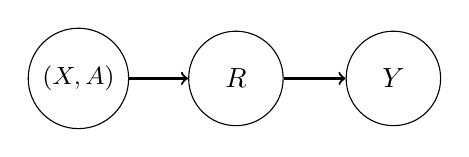
\begin{tikzpicture}

\node[circle,draw, minimum size=1.2cm] (R0) at (0,0) {\begin{small}$(X, A)$\end{small}
};
\node[circle,draw, minimum size=1.2cm] (R1) at (2,0) {$R$};
\node[circle,draw, minimum size=1.2cm] (Y) at (4,0) {$Y$};

\path[->, thick] (R0) edge (R1);
\path[->, thick] (R1) edge (Y);

\end{tikzpicture}
\caption{Bayesian network corresponding to Assumption \ref{assum:indep-general}.}
\label{fig:embedding_single}
% \vspace{-0.5cm}
% \end{wrapfigure}
\end{figure}
As illustrated in Figure \ref{fig:embedding_single}, Assumption \ref{assum:indep-general} means that the embedding $R$ fully mediates every possible effect of $(X, A)$ on $Y$. The generalised MIPS estimator $\hat{\theta}_{\textup{G-MIPS}}$ of target policy value, $\Etar[Y]$, is defined as
\[
\hat{\theta}_{\textup{G-MIPS}} \coloneqq \frac{1}{n}\sum_{i=1}^n \frac{\ptar(r_i)}{\pbeh(r_i)}\, y_i,
\]
where $\pbeh(r)$ denote the density of $R$ under the behaviour policy (likewise for $\ptar(r)$). Under assumption \ref{assum:indep-general}, $\hat{\theta}_{\textup{G-MIPS}}$ provides an unbiased estimator of target policy value. 
Similar to Lemma \ref{lemma:weights-est}, the density ratio $\frac{\ptar(r)}{\pbeh(r)}$ can be estimated by solving the regression problem
\begin{align}
    \arg \min_f \Ebeh \left(\frac{\tar(A\mid X)}{\beh(A\mid X)} - f\left(R\right)\right)^2. \label{eq:embedding-ratio-estimation}
\end{align}

\subsection{Variance reduction of G-MIPS estimator}\label{app:gmips-var-reduction}
By only considering the shift in the embedding $R$, the G-MIPS estimator achieves a lower variance relative to the vanilla IPW estimator. The following result, which is a straightforward extension of \cite[Theorem 3.6]{saito2022off}, formalises this.

\begin{proposition}[Variance reduction of G-MIPS]\label{prop:mips_var_reduction}
    When the ratios $\rho(a, x)$ and $\frac{\ptar(r)}{\pbeh(r)}$ are known exactly then under Assumption \ref{assum:indep-general}, we have that $\Ebeh[\thetaipw] = \Ebeh[\hat{\theta}_{\textup{G-MIPS}}] = \Etar[Y]$. Moreover,
\begin{align*}
     \Vbeh[\thetaipw] - \Vbeh[\hat{\theta}_{\textup{G-MIPS}}]
    \geq \frac{1}{n}\Ebeh \left[ \E[Y^2\mid R] \Vbeh[\rho(A, X)\mid R] \right] \geq 0.
\end{align*}
\end{proposition}

\begin{proof}[Proof of Proposition \ref{prop:mips_var_reduction}]
The following proof, which is included for completeness, is a straightforward extension of \cite[Theorem 3.6]{saito2022off}. 
\begin{align*}
    &n (\Vbeh[\thetaipw] - \Vbeh[\hat{\theta}_{\textup{MIPS}}])\\
    &\quad= \Vbeh\left[\frac{\tar(A|X)}{\beh(A|X)}\,Y\right] - \Vbeh\left[\frac{\ptar(R)}{\pbeh(R)}\,Y \right]\\
     &\quad= \Vbeh\left[\Ebeh\left[\frac{\tar(A|X)}{\beh(A|X)}\,Y \Bigg| R\right]\right] + \Ebeh\left[ \Vbeh\left[\frac{\tar(A|X)}{\beh(A|X)}\,Y\Bigg| R \right]\right] - \Vbeh\left[\Ebeh\left[ \frac{\ptar(R)}{\pbeh(R)}\,Y \Bigg| R\right]\right]\\
     &\qquad- \Ebeh\left[\Vbeh\left[ \frac{\ptar(R)}{\pbeh(R)}\,Y \Bigg| R\right]\right]
\end{align*}
Now using the conditional independence Assumption \ref{assum:indep-general}, the first term on the RHS above becomes,
\begin{align*}
    \Vbeh\left[\Ebeh\left[\frac{\tar(A|X)}{\beh(A|X)}\,Y \Bigg| R\right]\right] &= \Vbeh\left[\Ebeh\left[\frac{\tar(A|X)}{\beh(A|X)}\Bigg| R\right]\,\Ebeh\left[Y | R\right]\right]\\
    &= \Vbeh\left[\frac{\ptar(R)}{\pbeh(R)}\,\Ebeh\left[Y | R\right]\right],
\end{align*}
where in the last step above we use the fact that
\begin{align*}
    \Ebeh\left[\frac{\tar(A|X)}{\beh(A|X)}\Bigg| R\right] = \frac{\ptar(R)}{\pbeh(R)}.
\end{align*}
Putting this together, we get that
\begin{align}
    &n (\Vbeh[\thetaipw] - \Vbeh[\hat{\theta}_{\textup{MIPS}}]) \nonumber\\ 
    &\quad= \Ebeh\left[ \Vbeh\left[\frac{\tar(A|X)}{\beh(A|X)}\,Y\Bigg| R \right]\right] - \Ebeh\left[\Vbeh\left[ \frac{\ptar(R)}{\pbeh(R)}\,Y \Bigg| R\right]\right]. \label{eq:variance-difference}
\end{align}
Since we have that 
\begin{align*}
    \Ebeh\left[\frac{\tar(A|X)}{\beh(A|X)}\,Y\Bigg| R \right] = \Ebeh\left[\frac{\tar(A|X)}{\beh(A|X)}\Bigg| R \right]\,\Ebeh\left[Y| R \right] = \frac{\ptar(R)}{\pbeh(R)}\,\Ebeh\left[Y| R \right],
\end{align*}
Eq. \eqref{eq:variance-difference} becomes,
\begin{align*}
    &\Ebeh\left[ \Vbeh\left[\frac{\tar(A|X)}{\beh(A|X)}\,Y\Bigg| R \right]\right] - \Ebeh\left[\Vbeh\left[ \frac{\ptar(R)}{\pbeh(R)}\,Y \Bigg| R\right]\right] \\
    &\quad= \Ebeh\left[ \Ebeh\left[ \left(\frac{\tar(A|X)}{\beh(A|X)}\,Y \right)^2\Bigg| R  \right] - \Ebeh\left[ \left(\frac{\ptar(R)}{\pbeh(R)}\,Y \right)^2\Bigg| R \right] \right]\\
    &\quad= \Ebeh\left[ \Ebeh\left[ \left(\frac{\tar(A|X)}{\beh(A|X)} \right)^2 \Bigg| R  \right] \, \Ebeh\left[Y^2 | R  \right] - \left(\frac{\ptar(R)}{\pbeh(R)}\right)^2\,\Ebeh\left[Y^2 | R \right] \right]\\
    &\quad= \Ebeh\left[\Ebeh\left[Y^2 | R \right]\, \left( \Ebeh\left[ \left(\frac{\tar(A|X)}{\beh(A|X)} \right)^2 \Bigg| R  \right] - \left(\Ebeh\left[ \frac{\tar(A|X)}{\beh(A|X)} \Bigg| R  \right]\right)^2\, \right) \right]\\
    &\quad=\Ebeh\left[\Ebeh\left[Y^2 | R \right]\, \Vbeh\left[\frac{\tar(A|X)}{\beh(A|X)} \Bigg| R \right]\right].
\end{align*}
\end{proof}

\paragraph{Intuition}
Here, $R$ contains all relevant information regarding the outcome $Y$. Moreover, intuitively $R$ can be thought of as the state obtained by `filtering out' relevant information about $Y$ from $(X, A)$. Therefore, $R$ contains less `redundant' information regarding the outcome $Y$ as compared to the covariate-action pair $(X, A)$. As a result, the G-MIPS estimator which only considers the shift in the marginal distribution of $R$ due to the policy shift is more efficient than the IPW estimator, which considers the shift in the joint distribution of $(X, A)$ instead.
In fact, as the amount of `redundant' information regarding $Y$ decreases in the embedding $R$, the G-MIPS estimator becomes increasingly efficient with decreasing variance. We formalise this as follows:
\begin{assumption}\label{assum:two-embeddings}
    Assume there exist embeddings $R^{(1)}, R^{(2)}$ of the covariate-action pair $(X, A)$, with Bayesian network shown in Figure \ref{fig:embedding_double}. 
    This corresponds to the following conditional independence assumptions:
    \[
    R^{(2)} \indep (X, A) \mid R^{(1)}, \qquad \textup{and} \qquad Y \indep (R^{(1)}, X, A) \mid R^{(2)}.
    \]
\end{assumption}
\begin{figure}[h!]
\centering
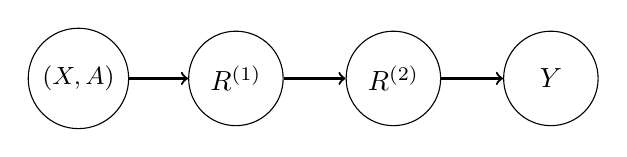
\begin{tikzpicture}

\node[circle,draw, minimum size=1.2cm] (R0) at (0,0) {\begin{small}$(X, A)$\end{small}};
\node[circle,draw, minimum size=1.2cm] (R1) at (2,0) {$R^{(1)}$};
\node[circle,draw, minimum size=1.2cm] (R2) at (4,0) {$R^{(2)}$};
\node[circle,draw, minimum size=1.2cm] (Y) at (6,0) {$Y$};

\path[->, thick] (R0) edge (R1);
\path[->, thick] (R1) edge (R2);
\path[->, thick] (R2) edge (Y);

\end{tikzpicture}
\caption{Bayesian network corresponding to Assumption \ref{assum:two-embeddings}.}
\label{fig:embedding_double}
\end{figure}  
% Here, $R^{(2)}$ can be thought of as the embedding obtained by `filtering out' relevant information about $Y$ from $R^{(1)}$, and as such $R^{(2)}$ contains less redundant information about $Y$ as compared to $R^{(1)}$. 
We can define G-MIPS estimators for these embeddings to obtain unbiased OPE estimators under Assumption \ref{assum:two-embeddings} as follows:
\[    \hat{\theta}^{(j)}_{\textup{G-MIPS}} \coloneqq \frac{1}{n}\sum_{i=1}^n \frac{\ptar(r_i^{(j)})}{\pbeh(r_i^{(j)})}\, y_i,
\]
for $j\in \{1, 2\}$. Here, $\frac{\ptar(r^{(j)})}{\pbeh(r^{(j)})}$ is the ratio of marginal densities of $R^{(j)}$ under target and behaviour policies. 
We next show that the variance of $\hat{\theta}^{(j)}_{\textup{G-MIPS}}$ decreases with increasing $j$.
\begin{proposition}\label{prop:mips_generalised}
    When the ratios $\rho(a, x)$, $w(y)$ and $\frac{\ptar(r^{(j)})}{\pbeh(r^{(j)})}$ are known exactly for $j \in \{1, 2\}$, then under Assumption \ref{assum:two-embeddings} we get that
    \[
    \Ebeh[\thetaipw] = \Ebeh[\hat{\theta}^{(1)}_{\textup{G-MIPS}}] = \Ebeh[\hat{\theta}^{(2)}_{\textup{G-MIPS}}] = \Ebeh[\thetamr] = \Etar[Y].
    \]
    Moreover, 
    \[
    \Vbeh[\thetaipw] \geq \Vbeh[\hat{\theta}^{(1)}_{\textup{G-MIPS}}] \geq  \Vbeh[\hat{\theta}^{(2)}_{\textup{G-MIPS}}] \geq \Vbeh[\thetamr].
    \]
\end{proposition}
\begin{proof}[Proof of Proposition \ref{prop:mips_generalised}]
    First, we prove that the G-MIPS estimators are unbiased using induction on $j$. We define $R^{(0)} \coloneqq (X, A)$ and $\hat{\theta}^{(0)}_{\textup{G-MIPS}}$ defined as
    \[
    \hat{\theta}^{(0)}_{\textup{G-MIPS}} \coloneqq \frac{1}{n}\sum_{i=1}^n \frac{\ptar(r_i^{(0)})}{\pbeh(r_i^{(0)})}\, y_i,
    \]
    recovers the IPW estimator $\thetaipw$. When $j=0$, we know that $\hat{\theta}^{(0)}_{\textup{G-MIPS}} = \thetaipw$ is unbiased. 
    Now, assume that $\Ebeh[\hat{\theta}^{(j)}_{\textup{G-MIPS}}] = \Etar[Y]$.

    Conditional on $R^{(j)}$, $R^{(j+1)}$ does not depend on the policy. Therefore, 
    \begin{align*}
        \frac{\ptar(r^{(j)})}{\pbeh(r^{(j)})} = \frac{\ptar(r^{(j)})\,p(r^{(j+1)}\mid r^{(j)}) }{\pbeh(r^{(j)})\,p(r^{(j+1)}\mid r^{(j)})} = \frac{\ptar(r^{(j)}, r^{(j+1)})}{\pbeh(r^{(j)}, r^{(j+1)})}.
    \end{align*}
    And therefore,
    \begin{align*}
        \frac{\ptar(r^{(j+1)})}{\pbeh(r^{(j+1)})} &= \int_{r^{(j)}} \frac{\ptar(r^{(j)}, r^{(j+1)})}{\pbeh(r^{(j)}, r^{(j+1)})} \, \pbeh(r^{(j)} \mid r^{(j+1)}) \,\mathrm{d} r^{(j)}\\ 
        &= \int_{r^{(j)}} \frac{\ptar(r^{(j)})}{\pbeh(r^{(j)})} \,\pbeh(r^{(j)} \mid r^{(j+1)}) \,\mathrm{d} r^{(j)}\\ 
        &= \Ebeh\left[\frac{\ptar(R^{(j)})}{\pbeh(R^{(j)})} \Bigg|  R^{(j+1)}=r^{(j+1)}\right].
    \end{align*}
    Using this and the fact that $R^{(j)}\indep Y \mid R^{(j+1)}$, we get that
    \begin{align*}
        \Ebeh\left[\hat{\theta}^{(j+1)}_{\textup{G-MIPS}} \right] &= \Ebeh\left[\frac{\ptar(R^{(j+1)})}{\pbeh(R^{(j+1)})}\, Y \right]\\
        &= \Ebeh\left[\frac{\ptar(R^{(j+1)})}{\pbeh(R^{(j+1)})}\, \Ebeh[Y| R^{(j+1)}] \right]\\
        &= \Ebeh\left[\Ebeh\left[\frac{\ptar(R^{(j)})}{\pbeh(R^{(j)})} \Bigg|  R^{(j+1)}\right]\, \Ebeh[Y| R^{(j+1)}] \right] \\
        &= \Ebeh\left[\Ebeh\left[\frac{\ptar(R^{(j)})}{\pbeh(R^{(j)})} \, Y \Bigg|  R^{(j+1)}\right]\right]\\
        &= \Ebeh\left[ \frac{\ptar(R^{(j)})}{\pbeh(R^{(j)})} \, Y \right]\\
        &= \Ebeh\left[\hat{\theta}^{(j)}_{\textup{G-MIPS}} \right] = \Etar[Y].
    \end{align*}
    Next, to prove the variance result we consider the difference
    \begin{align*}
        &\Vbeh[\hat{\theta}^{(j)}_{\textup{G-MIPS}}] - \Vbeh[\hat{\theta}^{(j+1)}_{\textup{G-MIPS}}] \\
        &= \frac{1}{n}\left(\Vbeh\left[\frac{\ptar(R^{(j)})}{\pbeh(R^{(j)})}\, Y\right] - \Vbeh\left[\frac{\ptar(R^{(j+1)})}{\pbeh(R^{(j+1)})}\, Y\right]\right) \\
        % &= \frac{1}{n}\left(\Vbeh\left[\frac{\ptar(R^{(j)})}{\pbeh(R^{(j)})}\, Y\right] - \Vbeh\left[\Ebeh\left[\frac{\ptar(R^{(j)})}{\pbeh(R^{(j)})} \Bigg|  R^{(j+1)}\right]\, Y\right]\right)\\
        &= \frac{1}{n}\Bigg(\Vbeh\left[ \Ebeh\left[\frac{\ptar(R^{(j)})}{\pbeh(R^{(j)})}\, Y \Bigg| R^{(j+1)} \right] \right] + \Ebeh\left[ \Vbeh\left[\frac{\ptar(R^{(j)})}{\pbeh(R^{(j)})}\, Y \Bigg| R^{(j+1)} \right] \right] \\
        &\qquad- \Vbeh\left[\frac{\ptar(R^{(j+1)})}{\pbeh(R^{(j+1)})}\, \Ebeh[Y\mid R^{(j+1)}]\right] - \Ebeh \left[\left(\frac{\ptar(R^{(j+1)})}{\pbeh(R^{(j+1)})}\right)^2\,\Vbeh[Y\mid R^{(j+1)}] \right] \Bigg)
    \end{align*}
    where in the last step we use the law of total variance. Now, using the fact that $R^{(j)}\indep Y \mid R^{(j+1)}$, we can rewrite the expression above as
    \begin{align*}
        &= \frac{1}{n}\Bigg(\Vbeh\left[ \Ebeh\left[\frac{\ptar(R^{(j)})}{\pbeh(R^{(j)})}\Bigg| R^{(j+1)} \right]\, \Ebeh[Y | R^{(j+1)} ] \right] + \Ebeh\left[ \Vbeh\left[\frac{\ptar(R^{(j)})}{\pbeh(R^{(j)})}\, Y \Bigg| R^{(j+1)} \right] \right] \\
        &\qquad- \Vbeh\left[\frac{\ptar(R^{(j+1)})}{\pbeh(R^{(j+1)})}\, \Ebeh[Y\mid R^{(j+1)}]\right] - \Ebeh \left[\left(\frac{\ptar(R^{(j+1)})}{\pbeh(R^{(j+1)})}\right)^2\,\Vbeh[Y\mid R^{(j+1)}] \right] \Bigg)\\
        &= \frac{1}{n}\Bigg( \Ebeh\left[ \Vbeh\left[\frac{\ptar(R^{(j)})}{\pbeh(R^{(j)})}\, Y \Bigg| R^{(j+1)} \right] \right] - \Ebeh \left[\left(\frac{\ptar(R^{(j+1)})}{\pbeh(R^{(j+1)})}\right)^2\,\Vbeh[Y\mid R^{(j+1)}] \right]\Bigg).
    \end{align*}
    Moreover, again using the conditional independence $R^{(j)}\indep Y \mid R^{(j+1)}$, we can expand the first term in the expression above as follows:
    % \begin{align*}
    %     \Vbeh\left[ \Ebeh\left[\frac{\ptar(R^{(j)})}{\pbeh(R^{(j)})}\, Y \Bigg| R^{(j+1)} \right] \right] &=
    %     \Vbeh\left[ \Ebeh\left[\frac{\ptar(R^{(j)})}{\pbeh(R^{(j)})}\Bigg| R^{(j+1)}\right]\, \Ebeh\left[Y | R^{(j+1)} \right] \right]\\
    %     &= \Vbeh\left[ \frac{\ptar(R^{(j+1)})}{\pbeh(R^{(j+1)})}\, \Ebeh\left[Y | R^{(j+1)} \right]\right]
    % \end{align*}
    \begin{align*}
        \Ebeh\left[ \Vbeh\left[\frac{\ptar(R^{(j)})}{\pbeh(R^{(j)})}\, Y \Bigg| R^{(j+1)} \right] \right] &=
        \Ebeh\Bigg[ \Ebeh\left[\frac{\ptar^2(R^{(j)})}{\pbeh^2(R^{(j)})} \Bigg| R^{(j+1)} \right]\,\Ebeh[Y^2 | R^{(j+1)}] \\
        &\qquad- \left(\Ebeh\left[\frac{\ptar(R^{(j)})}{\pbeh(R^{(j)})} \Bigg| R^{(j+1)} \right] \Ebeh[Y | R^{(j+1)}] \right)^2 \Bigg]\\
        &\geq 
        \Ebeh\Bigg[ \left(\Ebeh\left[\frac{\ptar(R^{(j)})}{\pbeh(R^{(j)})} \Bigg| R^{(j+1)} \right]\right)^2 \,\Ebeh[Y^2 | R^{(j+1)}] \\
        &\qquad- \left(\frac{\ptar(R^{(j+1)})}{\pbeh(R^{(j+1)})} \Ebeh[Y | R^{(j+1)}] \right)^2 \Bigg]\\
        &= \Ebeh\Bigg[ \left(\frac{\ptar(R^{(j+1)})}{\pbeh(R^{(j+1)})}\right)^2 \, \Vbeh[Y\mid R^{(j+1)}] \Bigg].
    \end{align*}
    Here, to get the inequality above, we use the fact that $\E[X^2] \geq (\E[X])^2$. Putting this together, we get that $\Vbeh[\hat{\theta}^{(j)}_{\textup{G-MIPS}}] - \Vbeh[\hat{\theta}^{(j+1)}_{\textup{G-MIPS}}] \geq 0$.

    Moreover, the result $\Vbeh[\hat{\theta}^{(2)}_{\textup{G-MIPS}}] \geq \Vbeh[\thetamr]$ follows straightforwardly from above by defining $R^{(3)} \coloneqq Y$. Then, the embeddings satisfy the causal structure 
    \[
    R^{(0)} \rightarrow R^{(1)} \rightarrow R^{(2)}  \rightarrow R^{(3)} \rightarrow Y.
    \]
    Using the result above, we know that $\Vbeh[\hat{\theta}^{(2)}_{\textup{G-MIPS}}] \geq \Vbeh[\hat{\theta}^{(3)}_{\textup{G-MIPS}}]$. But now it is straightforward to see that $\hat{\theta}^{(3)}_{\textup{G-MIPS}} = \thetamr$, and the result follows.
\end{proof}

\paragraph{Intuition}
Here, $R^{(j+1)}$ can be thought of as the embedding obtained by `filtering out' relevant information about $Y$ from $R^{(j)}$. As such, the amount of `redundant' information regarding the outcome $Y$ decreases successively along the sequence $R^{(0)} (\coloneqq (X, A)), R^{(1)}, R^{(2)}$. As a result, the G-MIPS estimators which only consider the shift in the marginal distributions of $R^{(j)}$ due to policy shift become increasingly efficient with decreasing variance as $j$ increases. Define the representation $R^{(3)} \coloneqq Y$, then the corresponding G-MIPS estimator reduces to the MR estimator, i.e., $\hat{\theta}^{(3)}_{\textup{G-MIPS}} = \thetamr$. Moreover, this estimator has minimum variance among all the G-MIPS estimators $\{\hat{\theta}^{(j)}_{\textup{G-MIPS}}\}_{0\leq j\leq k}$, as the representation $R^{(3)}$ contains precisely the least amount of information necessary to obtain the outcome $Y$. In other words, $Y$ itself serves as the `best embedding' of covariate-action pair $R^{(0)}$ which contains all relevant information regarding $Y$. We verify this empirically in Appendix \ref{subsec:mips-empirical} by reproducing the experimental setup in \cite{saito2022off} along with the MR baseline. Additionally, the MR estimator does not rely on assumptions like \ref{assum:indep-general} for unbiasedness. 

In addition to this, solving the regression problem in Eq. \eqref{eq:embedding-ratio-estimation} will typically be more difficult when $R$ is higher dimensional (as is likely to be the case for many choices of embeddings $R$), leading to high bias. In contrast, for MR the embedding $R=Y$ is one dimensional and therefore the regression problem is significantly easier to solve and yields lower bias. Our empirical results in Appendix \ref{app:experiments} confirm this.

\subsection{Doubly robust G-MIPS estimators}
Consider the setup for the G-MIPS estimator shown in Figure \ref{fig:embedding_single}. In this case, we can derive a doubly robust extension of the G-MIPS estimator, denoted as GM-DR, which uses an estimate of the conditional mean $\tilde{\mu}(r) \approx \E[Y\mid R=r]$ as a control variate to decrease the variance of G-MIPS estimator. This can be explicitly written as follows:
\begin{align}
\thetagmdr \coloneqq \frac{1}{n} \sum_{i=1}^n \frac{\ptar(r_i)}{\pbeh(r_i)}\,(y_i - \tilde{\mu}(r_i)) + \tilde{\eta}(\tar). \label{eq:gmips-dr}    
\end{align}
where $\tilde{\eta}(\tar) = \frac{1}{n} \sum_{i=1}^n \sum_{r' \in \mathcal{R}} \tilde{\mu}(r') \, \ptar(r' \mid x_i)$ is the analogue of the direct method. Here, $\mathcal{R}$ denotes the space of the possible of the representations $R$\footnote{the $\sum_{r' \in \mathcal{R}}$ can be replaced with $\int_{r' \in \mathcal{R}} \mathrm{d}r'$ when $\mathcal{R}$ is continuous}. Moreover, given the density $p(r \mid x, a)$, we can compute $\ptar(r\mid x)$ using
\[
\ptar(r\mid x) = \sum_{a' \in \Aspace} p(r \mid x, a')\,\tar(a'\mid x).
\]
It is straightforward to extend ideas from \cite{dudik2014doubly} to show that estimator $\thetagmdr$ is doubly robust in that it will yield accurate value estimates if either the importance weights $\frac{\ptar(r)}{\pbeh(r)}$ or the outcome model $\tilde{\mu}(r)$ is well estimated. 

\paragraph{There is no analogous DR extension of the MR estimator}
A consequence of considering the embedding $R=Y$ (as in MR) is that in this case we do not have an analogous doubly robust extension as above. To see why this is the case, note that when $R=Y$, we get that $\tilde{\mu}(r) = \E[Y\mid R=r] = \E[Y\mid Y=y] = y$. If we substitute this $\tilde{\mu}(r)$ in \eqref{eq:gmips-dr}, we are simply left with $\tilde{\eta}(\tar)$ on the right hand side (as the first term cancels out). This means that the resulting estimator does not retain the doubly robust nature as we no longer obtain an accurate estimate if either the outcome model or the importance ratios are well estimated.
% Additionally, $\tilde{\eta}(\tar)$ is an accurate estimate of the policy estimate only in the case when we have a good estimate of $\ptar(y\mid x)$.
% This is a non-trivial distribution to estimate as we do not have reward samples from the target distribution. Moreover, this also means that the resulting estimator does not retain the doubly robust nature as we no longer obtain an accurate estimate if either the outcome model or the importance ratios are well estimated.


% \newpage
\section{Application to causal inference}\label{app:causal-inference}
In this section, we investigate the application of the MR estimator for the estimation of average treatment effect (ATE). In this setting, we suppose that $\Aspace = \{0, 1\}$, and the goal is to estimate ATE defined as follows:
\[
\ate \coloneqq \E[Y(1)-Y(0)]
\]
Here, we use the potential outcomes notation \citep{robins1986new} to denote the outcome under a deterministic policy $\tar(a'\mid x) = \mathbbm{1}(a'=a)$ as $Y(a)$. 

Specifically, the IPW estimator applied to ATE estimation yields:
\[
\ateipw = \frac{1}{n} \sum_{i=1}^n \rho_{\ate}(a_i, x_i) \times y_i,
\]
where 
\[
\rho_{\ate}(a, x) \coloneqq \frac{\mathbbm{1}(a=1) - \mathbbm{1}(a=0)}{\beh (a|x)}.
\]
Similarly, the MR estimator can be written as
\[
\atemr = \frac{1}{n}\sum_{i=1}^n w_{\ate}(y_i)\times y_i, 
\]
where
\[
w_{\ate}(y) = \frac{p_{\pi^{(1)}}(y) - p_{\pi^{(0)}}(y)}{\pbeh(y)},
\] 
and $\pi^{(a)}(a'\mid x) \coloneqq \mathbbm{1}(a'=a)$ for $a\in \{0,1\}$.

Again, using the fact that $w_{\ate}(Y) \eqas \E[\rho_{\ate}(A, X)\mid Y]$, we can obtain $w_{\ate}$ by minimising a simple mean-squared loss:
\begin{align*}
    w_{\ate} =\arg \min_{f} \Ebeh \Big[\frac{\mathbbm{1}(A=1)- \mathbbm{1}(A=0)}{\beh (A|X)}-f(Y)\Big]^2.
\end{align*}
\begin{proposition}[Variance comparison with IPW ATE estimator]\label{prop:ate_variance}
When the weights $\rho_{\ate}(a, x)$ and $w_{\ate}(y)$ are known exactly, we have that $\V[\atemr] \leq \V[\ateipw]$. Specifically,
\begin{align*}
    \V[\ateipw] - \V[\atemr] = \frac{1}{n}\E\left[ \V\left[\rho_{\ate}(A, X) | Y \right]\,Y^2 \right] \geq 0.
\end{align*}
\end{proposition}
\begin{proof}[Proof of Proposition \ref{prop:ate_variance}] We have
\begin{align}
    \V[\ateipw] - \V[\atemr] &= \frac{1}{n}\left( \V[\rho_{\ate}(A, X)\, Y] - \V[w_{\ate}(Y)\,Y] \right). \label{eq:variance_ate_ipw_minus_mr}
\end{align}
Using the tower law of variance, we get that
\begin{align*}
    \V[\rho_{\ate}(A, X)\, Y] 
    &= \V[\E[\rho_{\ate}(A, X)\,  Y\mid Y]] + \E[\V[\rho_{\ate}(A, X)\, Y\mid Y]]\\
    &= \V[\E[\rho_{\ate}(A, X)\mid Y]\,  Y] + \E[\V[\rho_{\ate}(A, X)\mid Y]\,Y^2]\\
    &= \V[w_{\ate}(Y)\,Y] + \E[\V[\rho_{\ate}(A, X)\mid Y]\,Y^2].
\end{align*}
Putting this together with \eqref{eq:variance_ate_ipw_minus_mr} we obtain,
\begin{align*}
    \V[\ateipw] - \V[\atemr] &= \frac{1}{n} \E[\V[\rho_{\ate}(A, X)\mid Y]\,Y^2],
\end{align*}
which straightforwardly leads to the result.
\end{proof}

Given the above definitions, the IPW estimator for $\E[Y(a)]$ would only consider datapoints with $A=a$, as it weights the samples using the policy ratios $\mathbbm{1}(A=a)/\beh(A|X)$ which are only non-zero when $A=a$. 
This is however not the case with the MR estimator, as it uses the weights $\ptar(Y)/\pbeh(Y)$ which are not necessarily zero for $A\neq a$. Therefore, MR uses all evaluation datapoints $\D$ when estimating $\E[Y(a)]$. The MR estimator therefore leads to a more efficient use of evaluation data in this example. 
% The MR estimator, on the other hand, yields an unweighted average since $\ptar(Y)/\pbeh(Y)=1$, and more importantly, uses all datapoints when estimating $\E[Y(1)]$. The MR estimator therefore leads to a more efficient use of data in this example. 
% \faaiz{consider the comparison against DR estimator}

Likewise, the doubly robust (DR) estimator applied to ATE estimation yields,
\begin{align*}
    \atedr \coloneqq \frac{1}{n} \sum_{i=1}^n \rho_{\ate}(a_i, x_i)\,\left(y_i - \hat{\mu}(a_i, x_i)\right) + \frac{1}{n} \sum_{i=1}^n \left( \hat{\mu}(1, x_i)-  \hat{\mu}(0, x_i)\right),
\end{align*}
where $\hat{\mu}(a, x)\approx \E[Y\mid X=x, A=a]$. 
Like in classical off-policy evaluation, DR yields an accurate estimator of ATE when either the weights $\rho_{\ate}(a, x)$ or the outcome model i.e., $\hat{\mu}(a, x) = \E[Y\mid X=x, A=a]$, are well estimated.
However, despite this doubly robust nature of the estimator, we can show that the variance of the DR estimator may be higher than that of the MR estimator in many cases. The following result formalises this variance comparison between the DR and MR estimators, and is analogous to the result in Proposition \ref{prop:var_dr} derived for classical off-policy evaluation. 
\begin{proposition}[Variance comparison with DR ATE estimator]\label{prop:ate_var_dr}
    When the weights $\rho_{\ate}(a, x)$ and $w_{\ate}(y)$ are known exactly,
    \begin{align*}
    &\V[\atedr] - \V[\atemr]\\
    &\qquad \qquad \qquad \geq \frac{1}{n}\E \left[ \V\left[ \rho_\ate(A, X)\,Y \mid Y \right] -  \V\left[ \rho_\ate(A, X)\mu(A, X) \mid X \right] \right],
\end{align*}
where $\mu(A, X) \coloneqq \E[Y\mid X, A]$.
\end{proposition}

\begin{proof}[Proof of Proposition \ref{prop:ate_var_dr}]
Using the law of total variance, we get that
\begin{align*}
    n\,\V[\atedr] &= \V[\rho_\ate(A, X)\,(Y -\hat{\mu}(A, X)) + (\hat{\mu}(1, X) - \hat{\mu}(0, X))]\\
    &= \V[ \E[\rho_\ate(A, X)\,(Y -\hat{\mu}(A, X)) + (\hat{\mu}(1, X) - \hat{\mu}(0, X))\mid X, A]] \\
    &\qquad+ \E[\V[\rho_\ate(A, X)\,(Y -\hat{\mu}(A, X)) + (\hat{\mu}(1, X) - \hat{\mu}(0, X))\mid X, A]]\\
    &= \V[ \rho_\ate(A, X)\,(\mu(A, X) -\hat{\mu}(A, X)) + (\hat{\mu}(1, X) - \hat{\mu}(0, X))]\\
    &\qquad+ \E[\rho^2_\ate(A, X)\V[Y\mid X, A]].
\end{align*}
    Again, using the law of total variance we can rewrite the first term on the RHS above as,
    \begin{align*}
        &\V[ \rho_\ate(A, X)\,(\mu(A, X) -\hat{\mu}(A, X)) + (\hat{\mu}(1, X) - \hat{\mu}(0, X))]\\
        &\quad= \V[\E[ \rho_\ate(A, X)\,(\mu(A, X) -\hat{\mu}(A, X)) + (\hat{\mu}(1, X) - \hat{\mu}(0, X))\mid  X]] \\
        &\qquad+ \E[\V[ \rho_\ate(A, X)\,(\mu(A, X) -\hat{\mu}(A, X)) + (\hat{\mu}(1, X) - \hat{\mu}(0, X))\mid  X]] \\
        &\quad\geq  \V[\E[ \rho_\ate(A, X)\,(\mu(A, X) -\hat{\mu}(A, X)) + (\hat{\mu}(1, X) - \hat{\mu}(0, X))\mid  X]]\\
        &\quad=  \V[\E[ \rho_\ate(A, X)\,(\mu(A, X) -\hat{\mu}(A, X)) + \rho_\ate(A, X)\,\hat{\mu}(A, X)\mid  X]]\\
        &\quad=  \V[\E[ \rho_\ate(A, X)\,\mu(A, X)\mid  X]],
    \end{align*}
    where, in the second last step above we use the fact that 
    \[
    \E[\rho_\ate(A, X)\,\hat{\mu}(A, X)\mid  X] = \hat{\mu}(1, X) - \hat{\mu}(0, X).
    \]

    Putting this together, we get that
    \begin{align*}
        n\,\V[\atedr] \geq \V[\E[ \rho_\ate(A, X)\,\mu(A, X)\mid  X]] + \E[\rho^2_\ate(A, X)\V[Y\mid X, A]].
    \end{align*}
    Therefore, 
    \begin{align*}
        &n\,(\V[\atedr] - \V[\atemr]) \\
        &\quad\geq \V[\E[ \rho_\ate(A, X)\,\mu(A, X)\mid  X]] + \E[\rho^2_\ate(A, X)\V[Y\mid X, A]] - \V[w_\ate(Y)\,Y]\\
        &\quad= \V[\E[ \rho_\ate(A, X)\,\mu(A, X)\mid  X]] + \E[\V[\rho_\ate(A, X)\,Y\mid X, A]] - \V[w_\ate(Y)\,Y]\\
        &\quad= \V[\E[ \rho_\ate(A, X)\,\mu(A, X)\mid  X]] + \V[\rho_\ate(A, X)\, Y] - \V[\E[\rho_\ate(A, X)\,Y\mid X, A]]\\
        &\qquad- \V[w_\ate(Y)\,Y]\\
        &\quad= \V[\E[ \rho_\ate(A, X)\,\mu(A, X)\mid  X]] + \V[\E[\rho_\ate(A, X)\mid Y]\, Y] + \E[\V[\rho_\ate(A, X)\mid Y]\,Y^2]\\
        &\qquad- \V[\E[\rho_\ate(A, X)\,Y\mid X, A]]- \V[w_\ate(Y)\,Y]\\
        &\quad= \V[\E[ \rho_\ate(A, X)\,\mu(A, X)\mid  X]] + \V[w_\ate(Y)\, Y] + \E[\V[\rho_\ate(A, X)\mid Y]\,Y^2]\\
        &\qquad- \V[\E[\rho_\ate(A, X)\,Y\mid X, A]]- \V[w_\ate(Y)\,Y]\\
        &\quad= \V[\E[ \rho_\ate(A, X)\,\mu(A, X)\mid  X]]- \V[\E[\rho_\ate(A, X)\,Y\mid X, A]] + \E[\V[\rho_\ate(A, X)\mid Y]\,Y^2]\\
        &\quad= \V[\rho_\ate(A, X)\,\mu(A, X)] - \E[\V[\rho_\ate(A, X)\,\mu(A, X)\mid  X]] - \V[\rho_\ate(A, X)\,\mu(A, X)]\\
        &\qquad+ \E[\V[\rho_\ate(A, X)\mid Y]\,Y^2]\\
        &\quad= \E \left[ \V\left[ \rho_\ate(A, X) \mid Y \right]\, Y^2 -  \V\left[ \rho_\ate(A, X)\mu(A, X) \mid X \right] \right].
        % &\quad\geq \V[\E[ \rho_\ate(A, X)\,\mu(A, X)\mid  X]]- \V[\rho_\ate(A, X)\,\mu(A, X)] + \E[\V[\rho_\ate(A, X)\mid Y]\,Y^2]
    \end{align*}
\end{proof}

Proposition \ref{prop:ate_var_dr} shows that if $\V\left[Y\, \rho_\ate(A, X) \mid Y \right]$ is greater than $\V\left[ \rho_\ate(A, X)\mu(A, X) \mid X \right]$ on average, the variance of the MR estimator will be less than that of the DR estimator. Intuitively, this is likely to happen when the dimension of context space $\Xspace$ is high because in this case, the conditional variance over $X$ and $A$, $\V\left[Y\, \rho_\ate(A, X) \mid Y \right]$ is likely to be greater than the conditional variance over $A$, $\V\left[ \rho_\ate(A, X)\mu(A, X) \mid X \right]$.

% \newpage
\section{Experimental Results}\label{app:experiments}
In this section, we provide additional experimental details for the results presented in the main text. We also include extensive experimental results to provide further empirical evidence in favour of the MR estimator. 

\paragraph{Computational details}
We ran our experiments on Intel(R) Xeon(R) CPU E5-2690 v4 @ 2.60GHz with 8GB RAM
per core. We were able to use 150 CPUs in parallel to iterate over different configurations and seeds.
However, we would like to note that for each run our algorithms only requires 1 CPU and at most 30 minutes to run as our neural networks are relatively small. Throughout our experiments, whenever the outcome $Y$ was continuous, we used a fully connected neural network with three hidden layers with 512, 256 and 32 nodes respectively (and ReLU activation function) to estimate the weights $\hat{w}(y)$. On the other hand, when the outcome is discrete we can directly estimate $\hat{w}(y) \approx \E[\hat{\rho}(A, X)\mid Y=y]$ by calculating the sample mean of $\hat{\rho}(A, X)$ on samples with $Y=y$. Additionally, for each configuration of parameters in our experiments, we ran experiments for 10 different seeds (in \{0, 1, \ldots, 9\}).

\subsection{Alternative methodology of estimating MR}
In addition to the OPE baselines like IPW, DM and DR estimators considered in the main text, we also include empirically investigate an alternative methodology of estimating MR.
% results for MR estimated using an alternative methodology. 
Below we describe this methodology, denoted as `MR (alt)', in greater detail:
\subsubsection{MR (alt)}\label{sec:alt-estimation-method}
Recall our definition of MR estimator:
\[
\thetamr \coloneqq \frac{1}{n} \sum_{i=1}^n w(y_i)\,y_i.
\]
In the main text, we propose estimating the weights $w(y)$ first and using this to estimate $\thetamr$ using the above expression. Alternatively, we can estimate $h(y) \coloneqq y\,w(y)$ using 
\begin{align*}
    h = \arg\min_{f} \, \Ebeh \left[ \Bigg(Y\,\frac{\tar(A|X)}{\beh (A|X)}-f(Y)\Bigg)^2\right].
\end{align*}
Subsequently, the MR estimator can be written as:
\[
\thetamr = \frac{1}{n}\sum_{i=1}^n h(y_i).
\]
We refer to this alternative methodology as `MR-alt' and compare it empirically against the original methodology (which we simply refer to as `MR'). 
In general, it is difficult to say which of the two methods will perform better. Intuitively speaking, in cases where the behaviour of the quantity $Y\,\frac{\tar(A|X)}{\beh (A|X)}$ with varying $Y$ is `smoother' than that of $\frac{\tar(A|X)}{\beh (A|X)}$, the alternative method is expected to perform better. Our empirical results in the next sections show that the relative performance of the two methods varies for different data generating mechanisms.

% \subsubsection{Switch-DR estimator}\faaiz{duplication of these definitions}
% The original DR estimator can still have a high variance when the importance weights are large due to a large policy shift. Switch-DR \cite{wang2017optimal} aims to circumvent this problem by switching to DM when the importance weights are large:
% \[
% \thetaswitch \coloneqq \frac{1}{n} \sum_{i=1}^n \rho(a_i, x_i)\,(y_i - \hat{\mu}(a_i, x_i))\ind(\rho(a_i, x_i) \leq \tau) + \hat{\eta}(\tar)
% \]
% where $\tau \geq 0$ is a hyperparameter, $\hat{\mu}(a, x) \approx \E[Y \mid x, a]$ is the outcome model, and 
% \[
% \hat{\eta}(\tar) = \frac{1}{n} \sum_{i=1}^n \sum_{a'\in \Aspace} \hat{\mu}(a', x_i) \tar(a'\mid x_i) \approx \E_{\tar}[\hat{\mu}(A, X)].
% \]

% \subsubsection{Doubly Robust with Optimal Shrinkage (DRos)}
% DRos proposed by \citep{su2020doubly} uses new weights $\hat{\rho}_\lambda(a_i, x_i)$ which directly minimises sharp bounds on the MSE of the resulting estimator,
% \[
% \thetadros \coloneqq \frac{1}{n} \sum_{i=1}^n \hat{\rho}_\lambda(a_i, x_i)\,(y_i - \hat{\mu}(a_i, x_i)) + \hat{\eta}(\tar),
% \]
% where $\lambda \geq 0$ is a pre-defined hyperparameter and $\hat{\rho}_\lambda$ is defined as
% \[
% \hat{\rho}_\lambda(a, x) \coloneqq \frac{\lambda}{\rho^2(a, x) + \lambda}\, \rho(a, x).
% \]
% When $\lambda = 0$, $\hat{\rho}_\lambda(a, x) = 0$ leads to DM, whereas as $\lambda \rightarrow \infty$, $\hat{\rho}_\lambda(a, x) \rightarrow \rho(a, x)$ leading to DR.

\subsection{Synthetic data experiments}\label{subsec:mips-empirical}
Here, we include additional experimental details for the synthetic data experiments presented in Section \ref{sec:exp-synth} for completeness. For this experiment, we use the same setup as the synthetic data experiment in \cite{saito2022off}, reproduced by reusing their code with minor modifications. 


% To verify the theoretical results in Section \ref{subsec:mips-comparison}, we empirically compare the MR estimator with the MIPS estimator. To do this, we reproduce the experimental setup for the synthetic data experiment in \cite{saito2022off} by reusing their code. Below, we include the experimental details for completeness. 

\paragraph{Setup}
Here, we sample the $d$-dimensional context vectors $x$ from a standard normal distribution. 
The setup used also includes $3$-dimensional categorical action embeddings $E \in \mathcal{E}$, which are sampled from the following conditional distribution given action $A=a$,
\[
p(e\mid a) = \prod_{k=1}^{3}\frac{\exp{(\alpha_{a, e_{k}})}}{\sum_{e'\in \mathcal{E}_k} \exp{(\alpha_{a, e'})}},
\]
which is independent of the context $X$. $\{\alpha_{a, e_k}\}$ is a set of parameters sampled independently from the standard normal distribution. Each dimension of $\mathcal{E}$ has a cardinality of $10$, i.e., $\mathcal{E}_k = \{1, 2, \dots, 10\}$.

\paragraph{Reward function}
The expected reward is then defined as:
\[
q(x, e) = \sum_{k=1}^{3} \eta_k \cdot (x^T\, M\, x_{e_k} + \theta_x^T\, x + \theta_e^T\, x_{e_k}),
\]
where $M$, $\theta_x$ and $\theta_e$ are parameter matrices or vectors sampled from a uniform distribution with range $[-1, 1]$. $x_{e_k}$ is a context vector corresponding to the $k$-th dimension of the action embedding, which is unobserved to the estimators. $\eta_k$ specifies the importance of the $k$-th dimension of the action embedding, sampled from Dirichlet distribution so that $\sum_{k=1}^{3} \eta_k = 1$. 

\paragraph{Behaviour and target policies}
The behaviour policy $\beh$ is defined by applying the softmax function to $q(x, a) = \E[q(X, E)\mid A=a, X=x]$ as 
\[
\beh(a\mid x) = \frac{\exp{(-q(x, a))}}{\sum_{a'\in \Aspace}\exp{(-q(x, a'))}}.
\]
% where, like before, the $\beta$ parameter controls the optimality and entropy of the behaviour policy. 

For the target policy, we define the class of parametric policies,
\[
\pi^{\alpha^\ast}(a | x) = \alpha^\ast\,\ind(a = \arg\max_{a'\in \Aspace} q(x, a')) + \frac{1-\alpha^\ast}{|\Aspace|},
\]
where $\alpha^\ast \in [0, 1]$ controls the shift between the behaviour and target policies. As shown in the main text, as $\alpha^\ast \rightarrow 1$, the shift between behaviour and target policies increases.

\paragraph{Baselines}
In the main text, we compare MR with DM, IPW, DR and MIPS estimators. In addition to these baselines, here we also consider Switch-DR \citep{wang2017optimal} and DR with Optimistic Shrinkage (DRos) \citep{su2020doubly}.
Following \cite{saito2022off}, we use the random forest \citep{breiman2001machine} along with 2-fold cross-fitting \citep{newey2018cross} to obtain $\hat{q}(x, e)$ for DR and DM methods.
To estimate $\pbeh(a\mid x, e)$ for MIPS estimator, we use logistic regression. 
We also include the results for MR estimated using the alternative methodology described in Section \ref{sec:alt-estimation-method}. We refer to this as `MR (alt)'.
% We also include the results of MIPS with true importance weights as `MIPS (true)'. 

\paragraph{Estimation of behaviour policy $\hatbeh$ and marginal ratio $\hat{w}(y)$}
We do not assume that the true behaviour policy $\beh$ is known, and therefore estimate $\hatbeh$ using the available training data.
For the MR estimator, we estimate the behaviour policy using a random forest classifier trained on 50\% of the training data and use the rest of the training data to estimate the marginal ratios $\hat{w}(y)$ using multi-layer perceptrons (MLP). Moreover, for a fair comparison we use a different behaviour policy estimate $\hatbeh$ for all other baselines which is trained on the entire training data. 


\begin{figure}[h!]
    \centering
	\begin{subfigure}{0.8\textwidth}
	    \centering
	    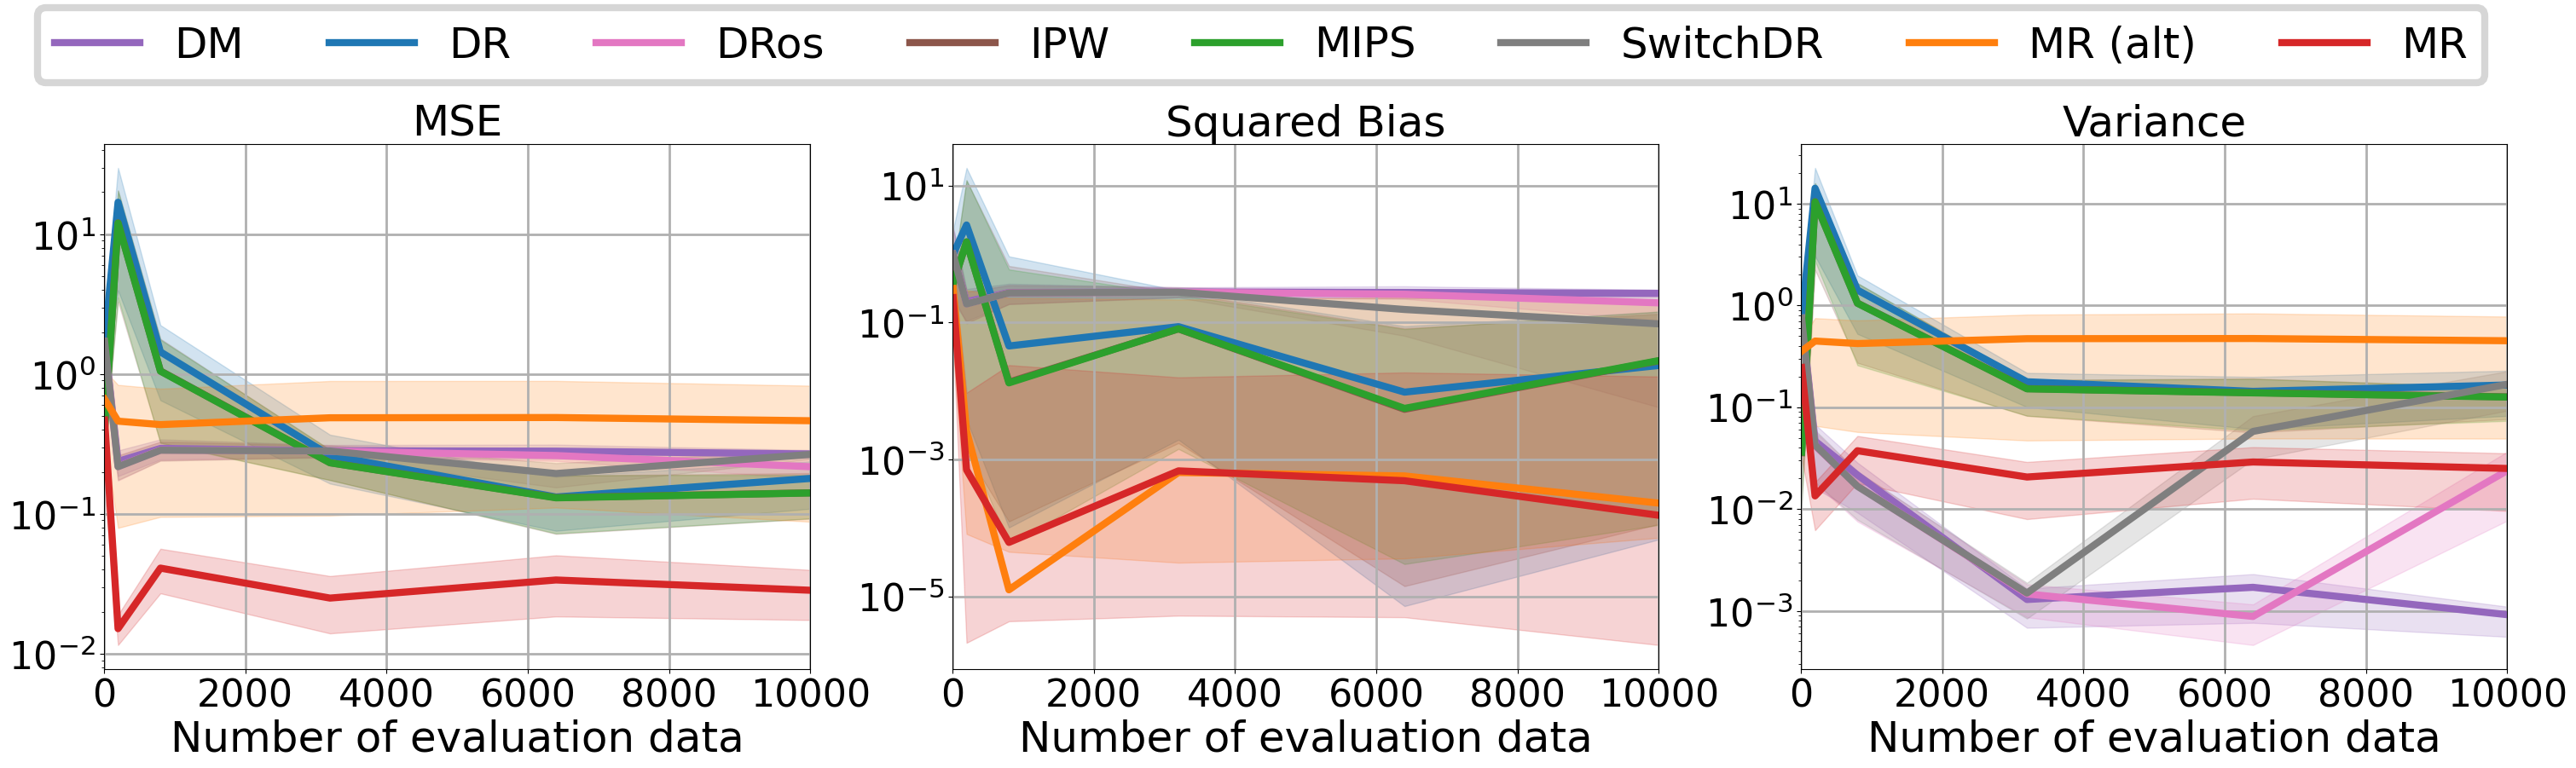
\includegraphics[width=1\textwidth]{figures/mr/mips_experiments/ope_vs_neval_nac_250_alphatar_0_8_dimc_5000.png}
	    \subcaption{$d=1000$, $n_{a}=100$, $\alpha^\ast = 0.8$}
	    \label{subfig:d-1000-na-250-neval-mips}
	\end{subfigure}\\
	\begin{subfigure}{0.8\textwidth} 
	    \centering
	    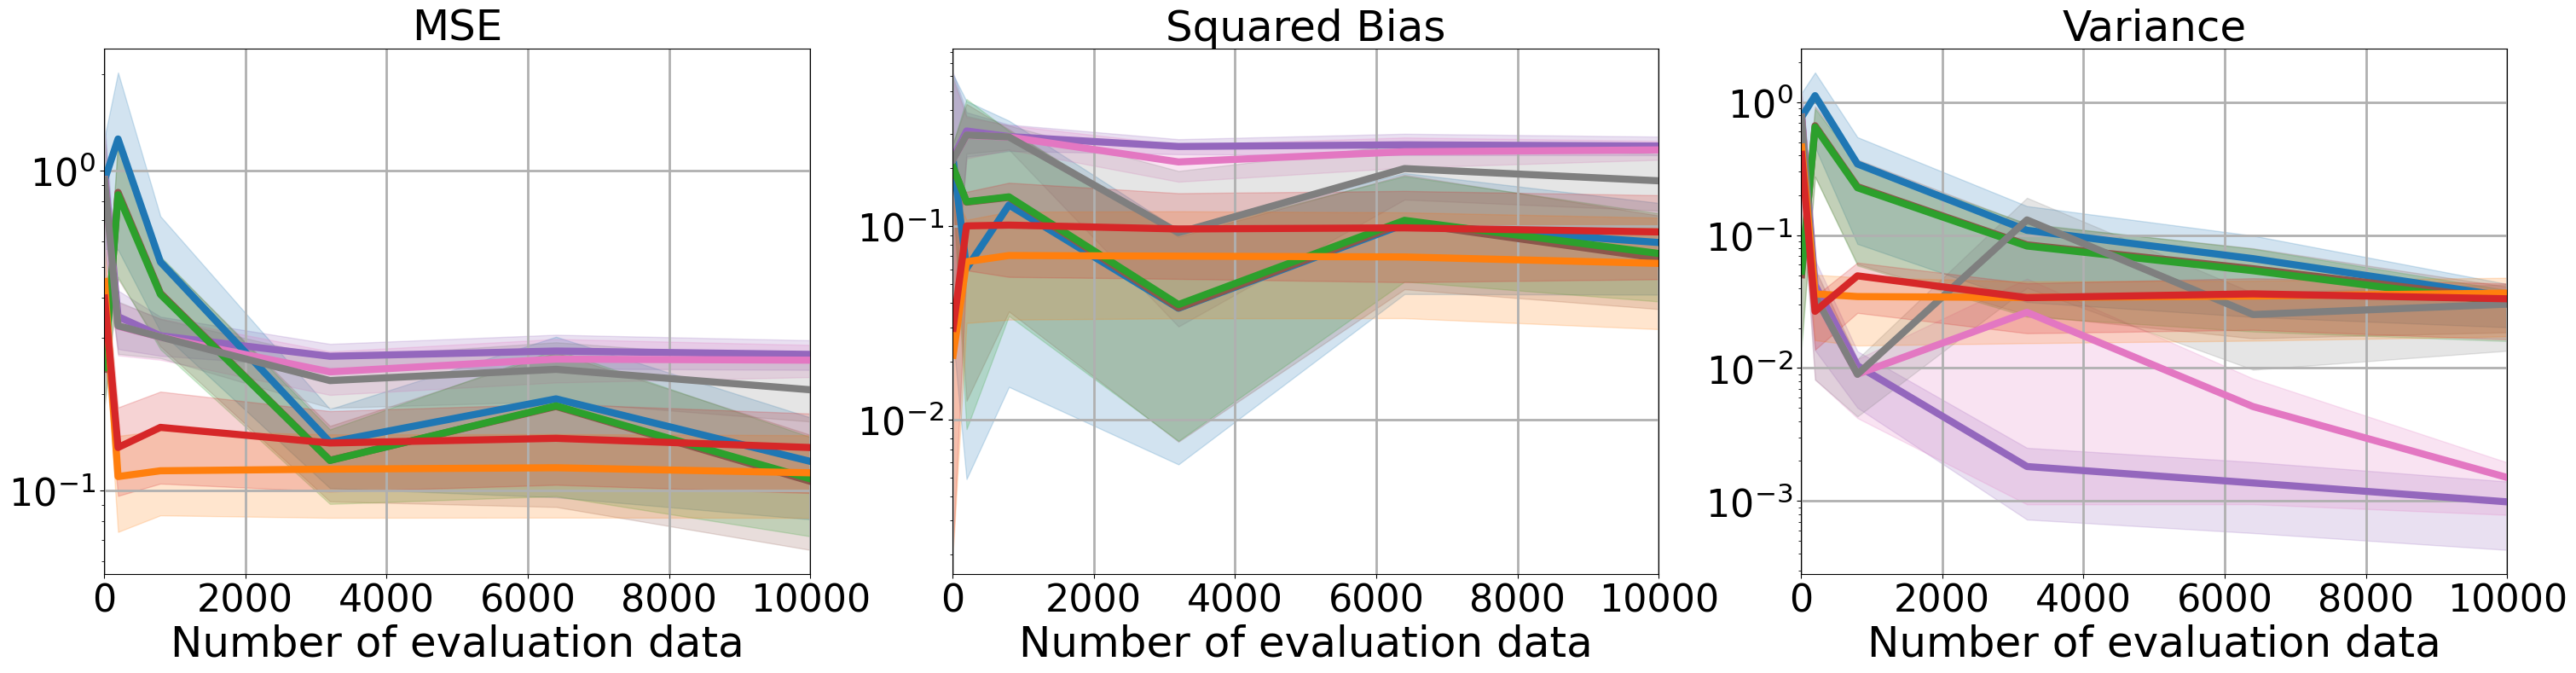
\includegraphics[width=1\textwidth]{figures/mr/mips_experiments/ope_vs_neval_nac_100_alphatar_0_8_dimc_1000.png}
	    \subcaption{$d=5000$, $n_{a}=250$, $\alpha^\ast = 0.8$}
	    \label{subfig:d-5000-na-250-neval-08-mips}
	\end{subfigure}\\
	\begin{subfigure}{0.8\textwidth} 
	    \centering
	    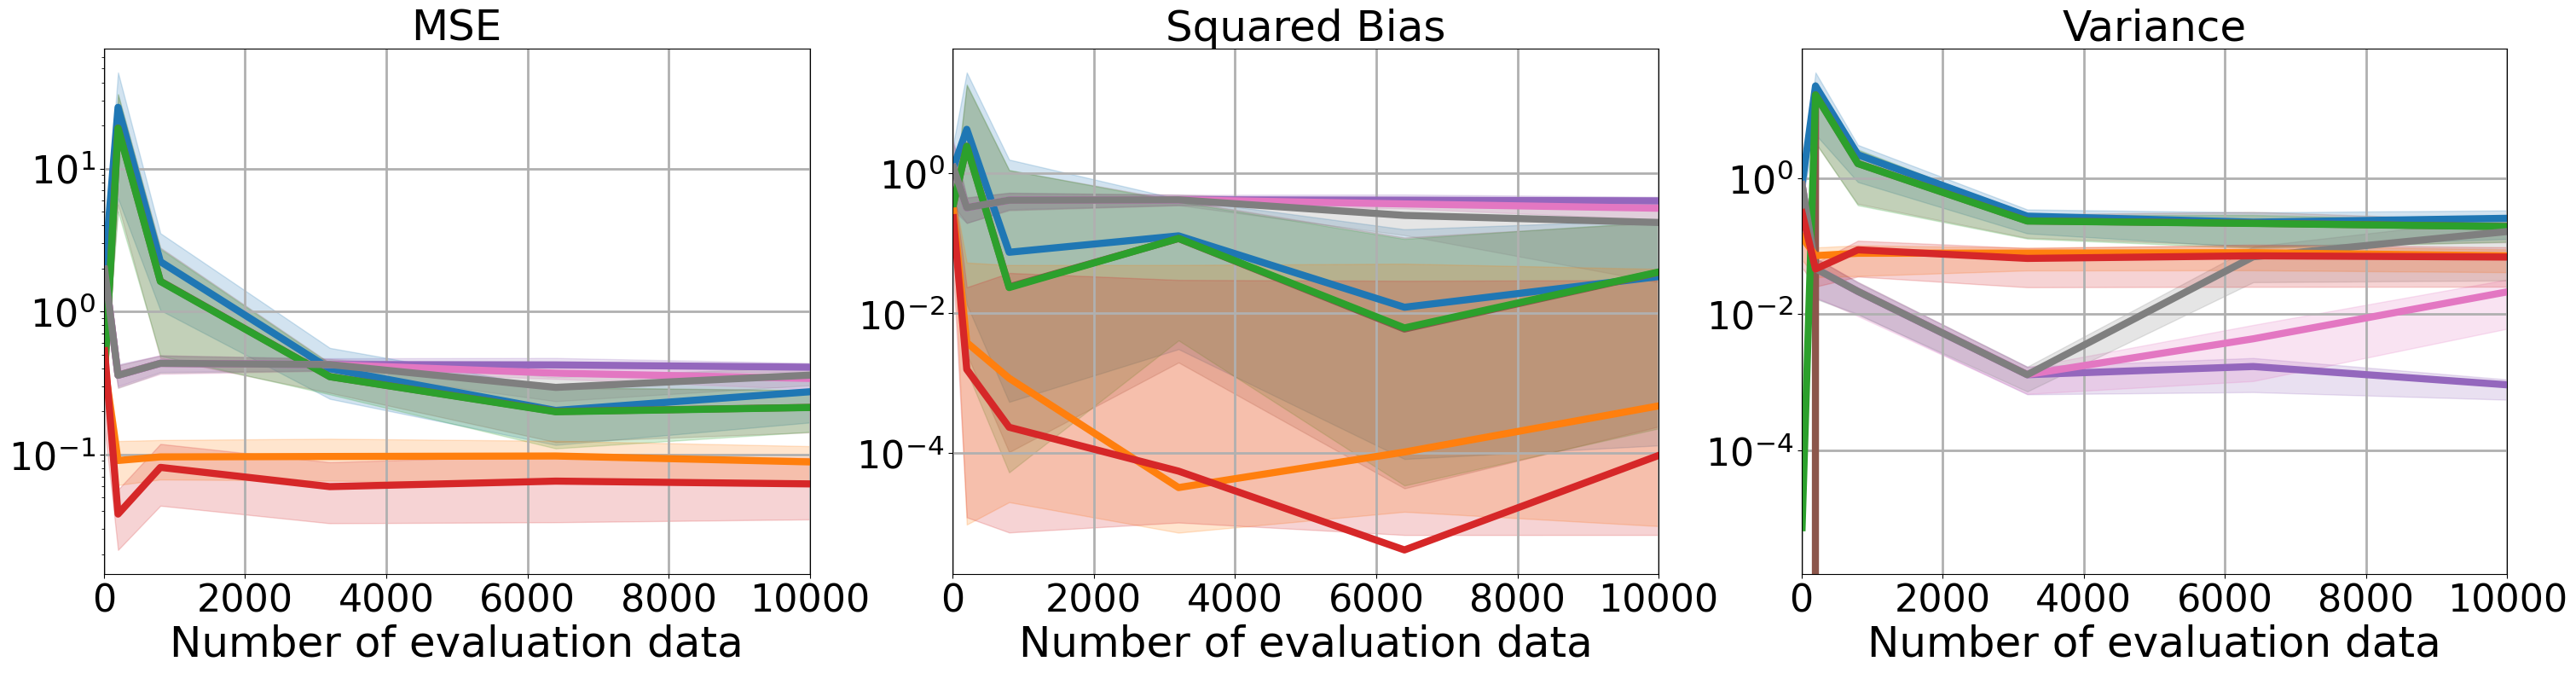
\includegraphics[width=1\textwidth]{figures/mr/mips_experiments/ope_vs_neval_nac_250_alphatar_1_0_dimc_5000.png}
	    \subcaption{$d=5000$, $n_{a}=250$, $\alpha^\ast = 1.0$}
	    \label{subfig:d-5000-na-250-neval-1-mips}
	\end{subfigure}
    \caption{MSE with varying size of evaluation dataset $n$ for different choices of parameters.}
    \label{fig:mse-vs-neval-mips}
\end{figure}

\begin{figure}[h!]
    \centering
	\begin{subfigure}{0.8\textwidth}
	    \centering
	    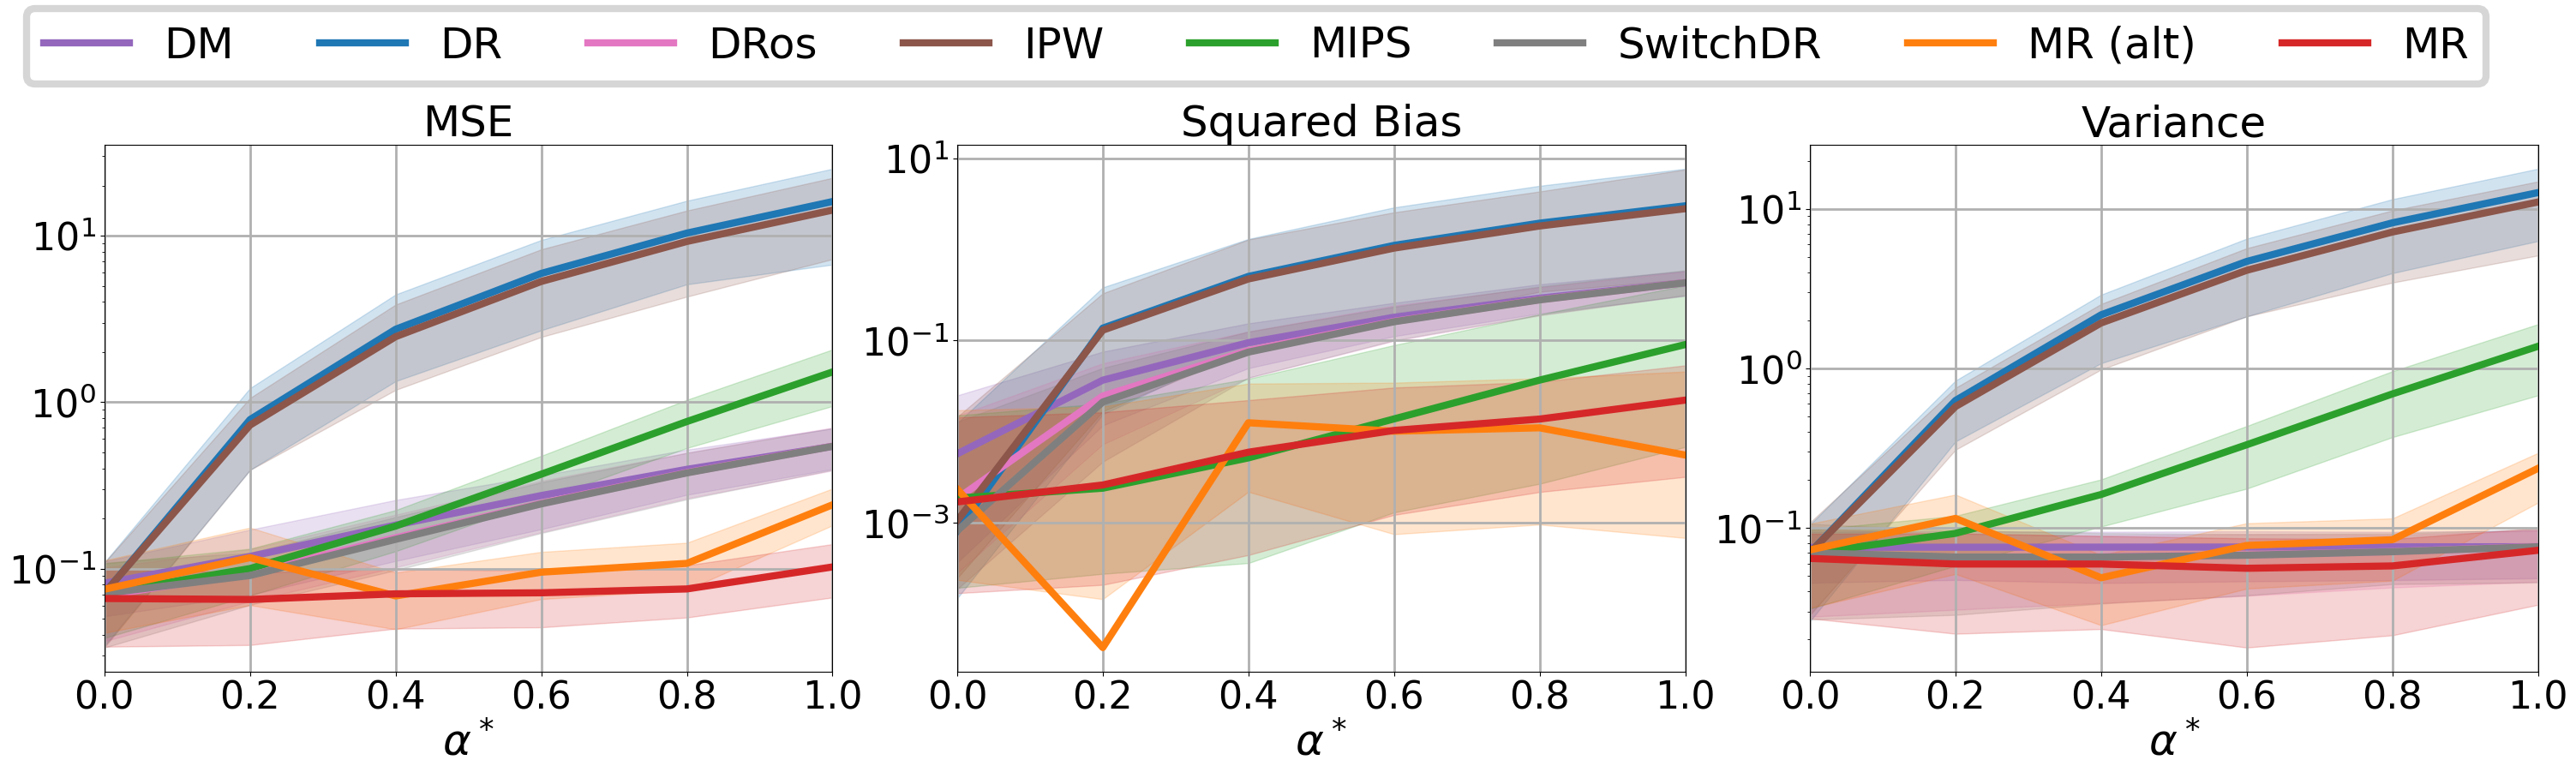
\includegraphics[width=1\textwidth]{figures/mr/mips_experiments/ope_vs_alphatar_dimc_100_neval_100_nac_100_ntrain_100000.png}
	    \subcaption{$d=100$, $n_{a}=100$, $n = 100$}
	    \label{subfig:d-100-na-100-neval-100-alphatar-mips}
	\end{subfigure}\\
	\begin{subfigure}{0.8\textwidth} 
	    \centering
	    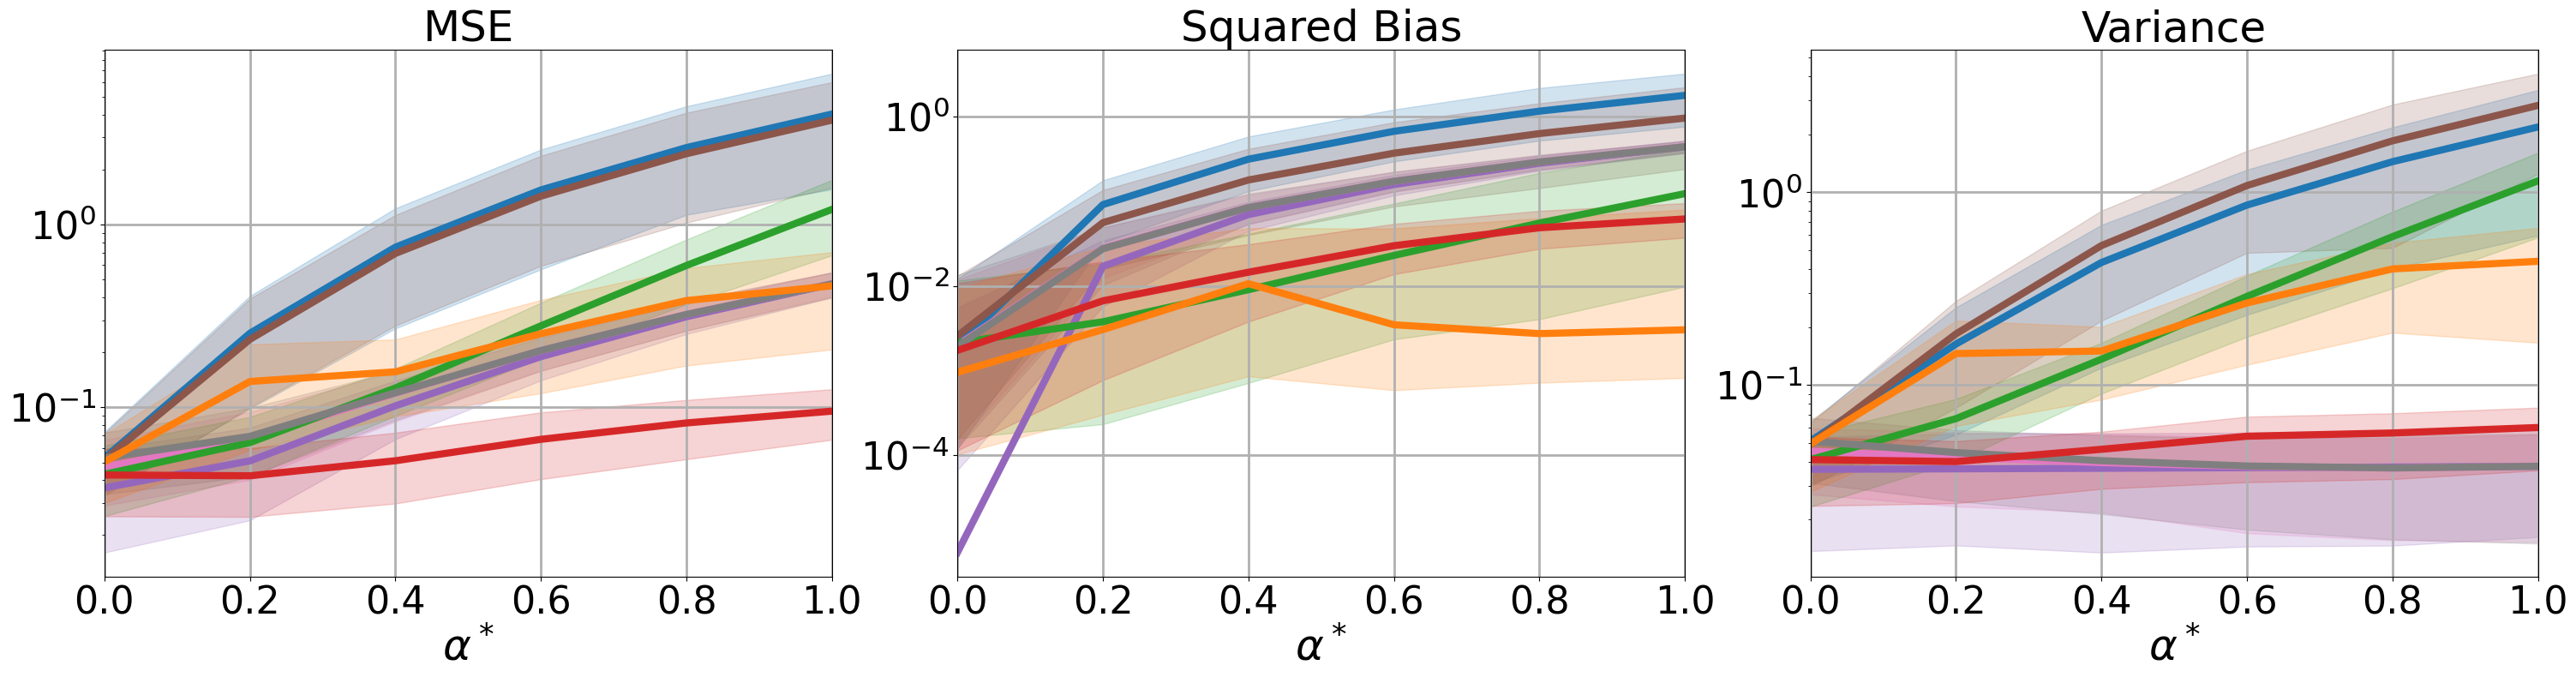
\includegraphics[width=1\textwidth]{figures/mr/mips_experiments/ope_vs_alphatar_dimc_100_neval_100_nac_250_ntrain_100000.png}
	    \subcaption{$d=100$, $n_{a}=250$, $n = 100$}
	    \label{subfig:d-100-na-250-neval-100-alphatar-mips}
	\end{subfigure}\\
	\begin{subfigure}{0.8\textwidth} 
	    \centering
	    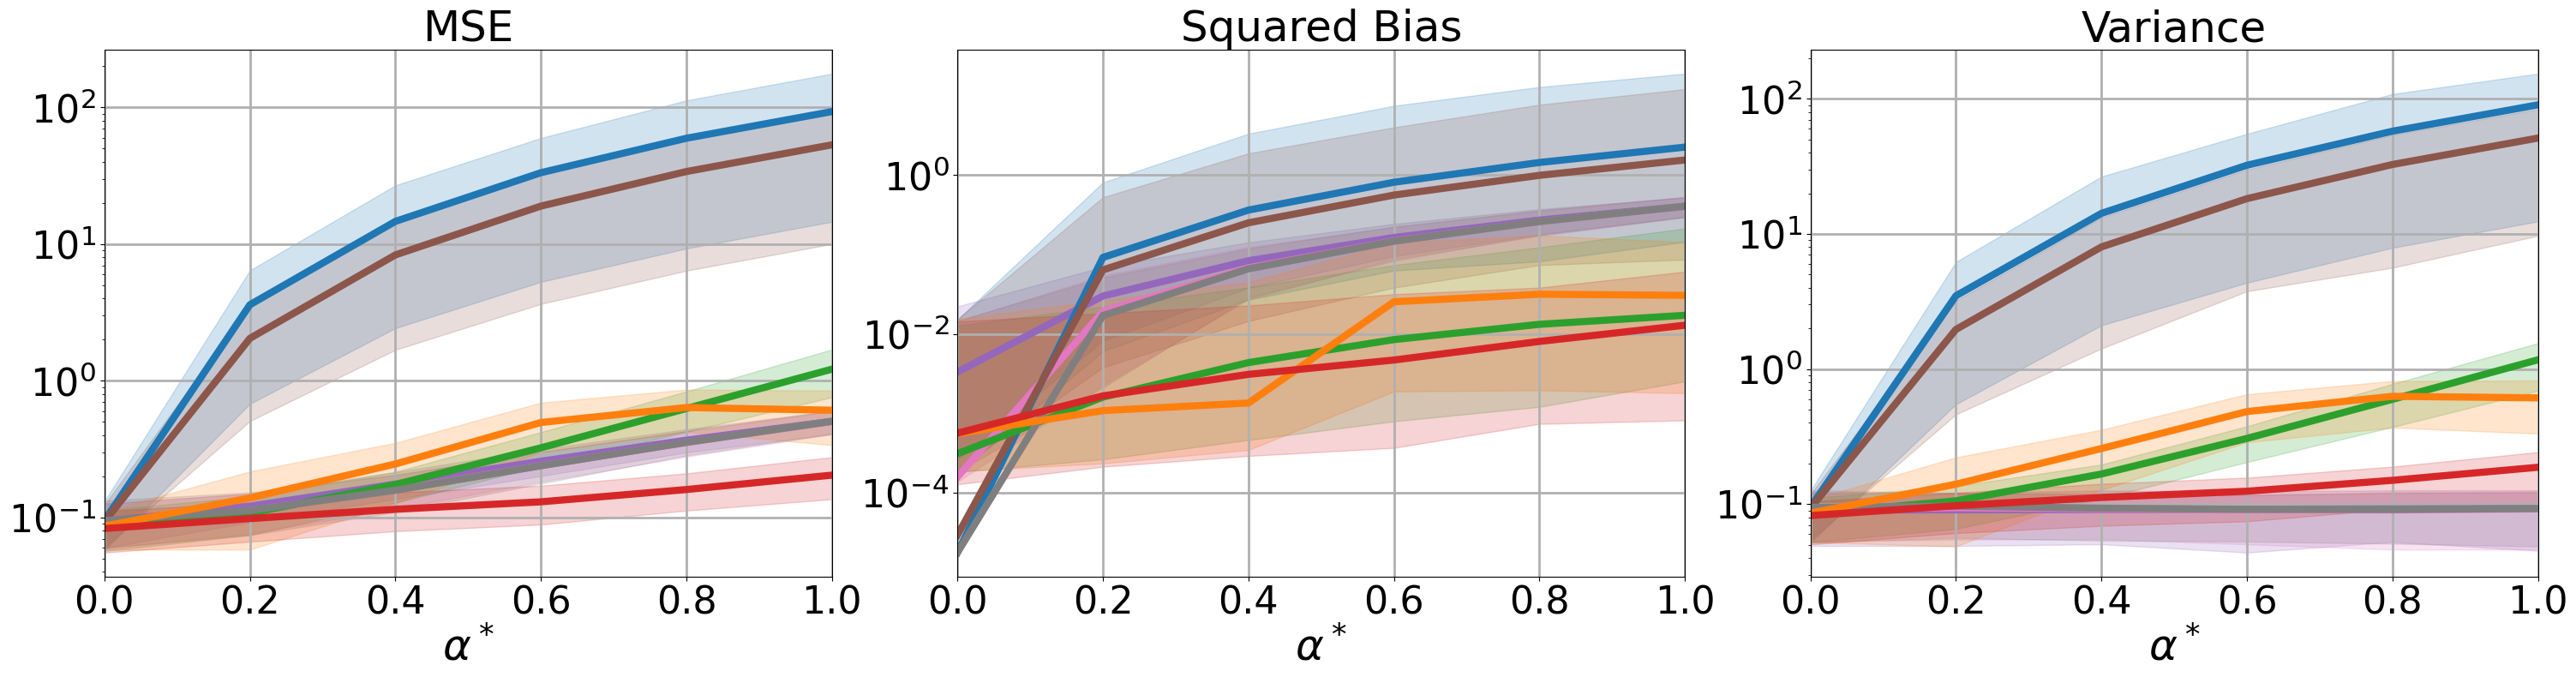
\includegraphics[width=1\textwidth]{figures/mr/mips_experiments/ope_vs_alphatar_dimc_1000_neval_100_nac_250_ntrain_100000.png}
	    \subcaption{$d=1000$, $n_{a}=250$, $n = 100$}
	    \label{subfig:d-1000-na-250-neval-100-alphatar-mips}
	\end{subfigure}
    \caption{MSE with varying $\alpha^\ast$ for different choices of parameters.}
    \label{fig:mse-vs-alphatar-mips}
\end{figure}

\subsubsection{Results}
For this experiment, the results are computed over 10 different sets of logged data replicated with different seeds, and in Figures \ref{fig:mse-vs-neval-mips} - \ref{fig:mse-vs-nac-mips} we use a total of $m=5000$ training data. 

\paragraph{Varying size of evaluation data $n$}
Figure \ref{fig:mse-vs-neval-mips} shows that MR outperforms the other baselines, in terms of MSE and squared bias, when the number of evaluation data $n\leq 1000$. Additionally, we observe that in this experiment, MR estimated using our original methods (`MR'), yields better results than the alternative method of estimating MR (`MR (alt)'). Moreover, while the variance of DM is lower than that of MR, the DM method has a high bias and consequently a high MSE. We note that while the difference between MSE and variance of MIPS and MR estimators decreases with increasing evaluation data size, MR still outperforms MIPS in terms of both MSE and variance.

\paragraph{Varying $\alpha^\ast$}
Figure \ref{fig:mse-vs-alphatar-mips} shows the results with increasing policy shift. It can be seen that overall MR methods achieve the smallest MSE with increasing policy shift. Moreover, the difference between MSE and variance of MR and IPW/DR methods increases with increasing policy shift, showing that MR performs especially better than these baselines when the difference between behaviour and target policies is large. Similarly, we observe in Figure \ref{fig:mse-vs-alphatar-mips} that as the shift between the behaviour and target policy increases with increasing $\alpha^\ast$, so does the difference between the MSE and variance of MR and the MIPS estimators. This shows that generally MR outperforms MIPS estimator in terms of variance and MSE, and that MR performs especially better than MIPS as the difference between behaviour and target policies increases.

\paragraph{Varying $d$ and $n_a$}
Figures \ref{fig:mse-vs-d-mips} and \ref{fig:mse-vs-nac-mips} show that MR outperforms the other baselines as the context dimensions and/or number of actions increase. In fact, these figures show that MR is significantly robust to increasing dimensions of action and context spaces, whereas baselines like IPW and DR perform poorly in large action spaces.

\paragraph{Varying $m$}
Figure \ref{fig:mse-vs-ntr-mips} shows the results with increasing number of training data $m$. We again observe that the MR methods `MR' and `MR (alt)' outperforms the other baselines in terms of the MSE and squared bias even when the number of training data is low. Moreover, the variance of both the MR estimators continues to improve with increasing number of training data.

In this experiment, we observe that overall `MR (alt)' performs worse than the original MR estimator (`MR' in the figures). However, as we observe in Appendix \ref{sec:app-additional-results}, this does not happen consistently across all experiments, which suggests that the comparative performance of the two MR methods depends on the data generating mechanism. 




\begin{figure}[h!]
    \centering
	\begin{subfigure}{0.8\textwidth}
	    \centering
	    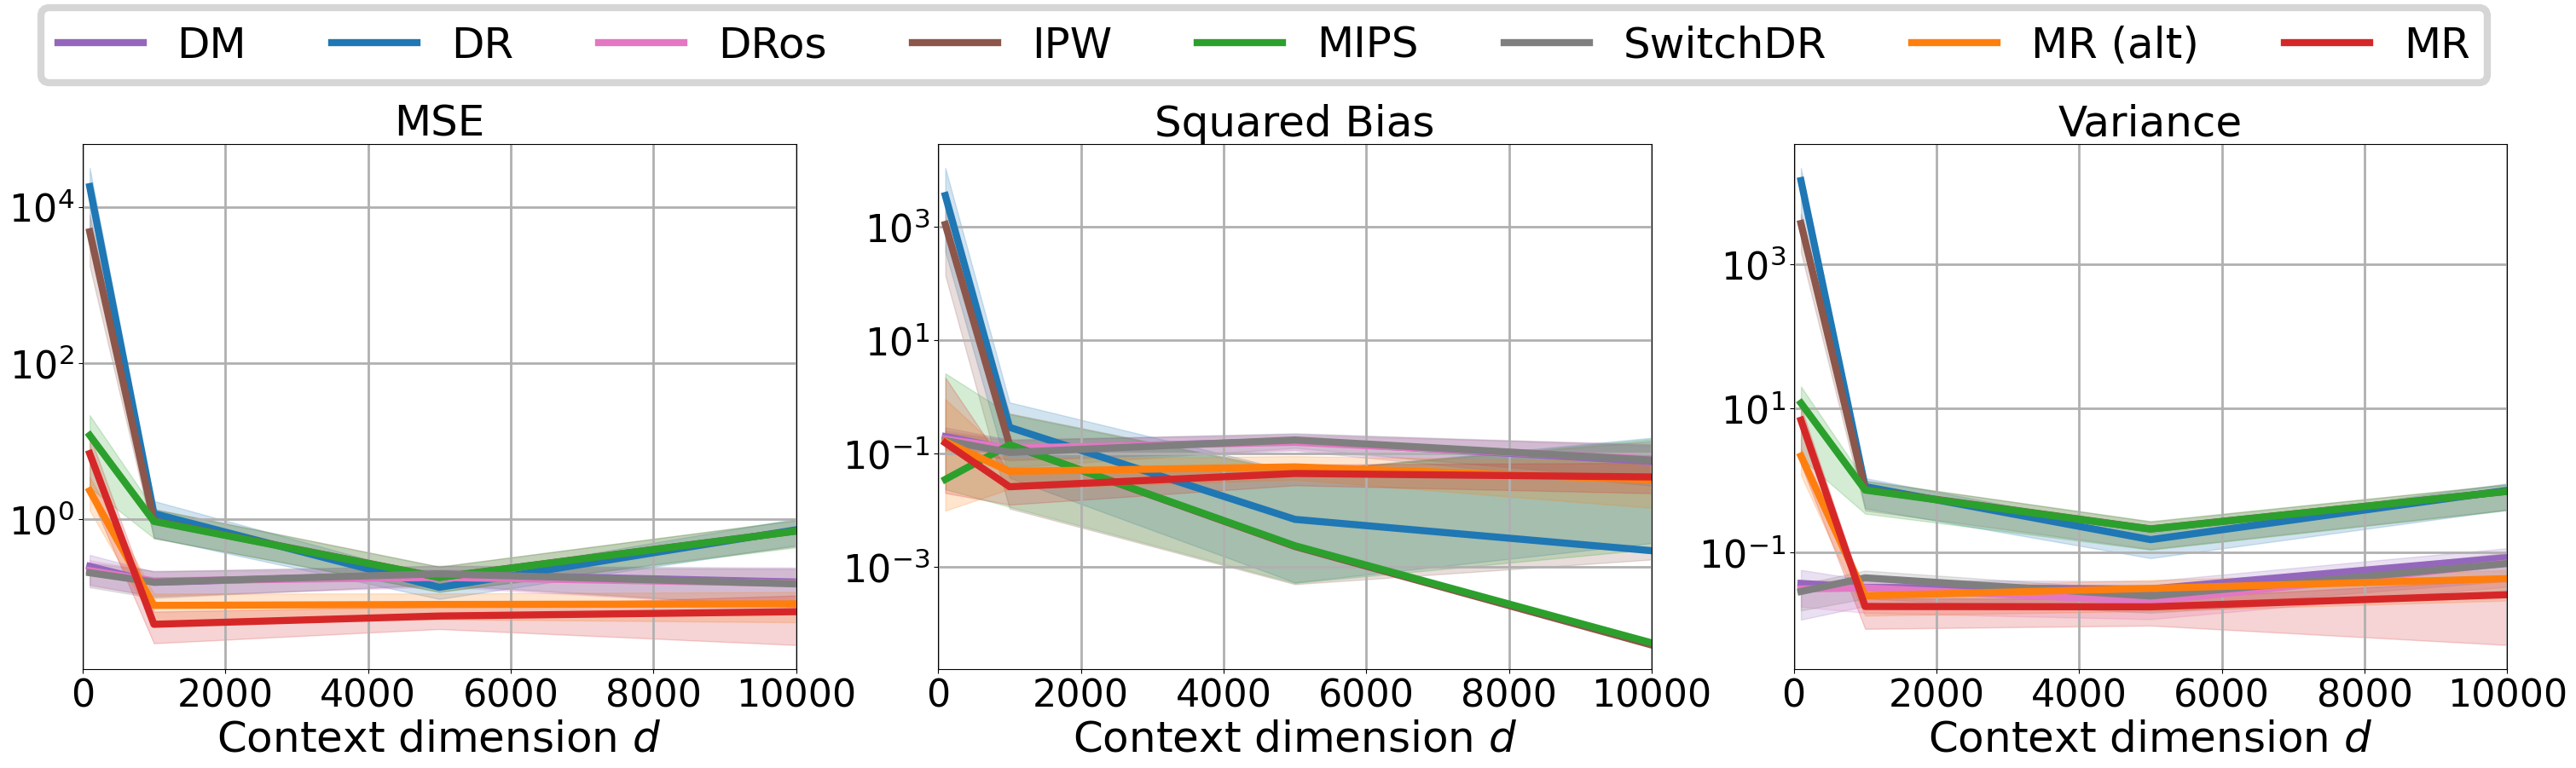
\includegraphics[width=1\textwidth]{figures/mr/mips_experiments/ope_vs_d_nac_20_alphatar_0_8_n_200.png}
	    \subcaption{$n_{a}=20$, $n = 200$, $\alpha^\ast = 0.8$}
	    \label{subfig:na-20-neval-200-alphatar-0-8-d-mips}
	\end{subfigure}\\
	\begin{subfigure}{0.8\textwidth} 
	    \centering
	    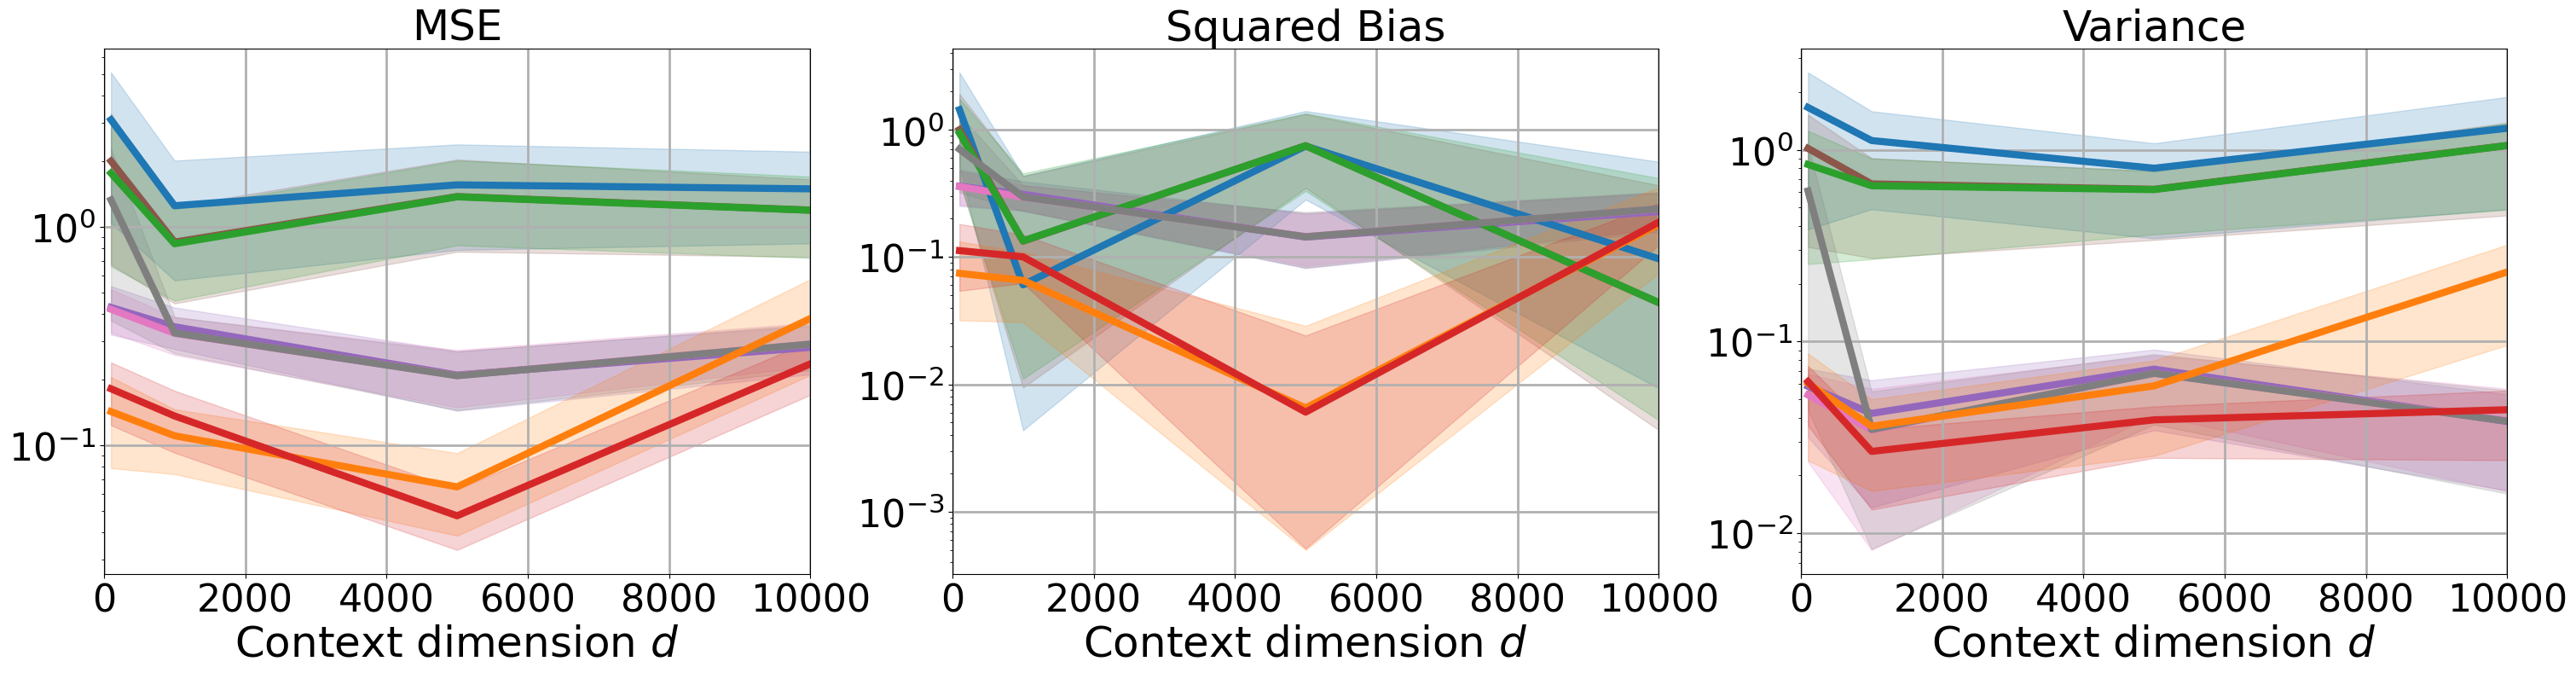
\includegraphics[width=1\textwidth]{figures/mr/mips_experiments/ope_vs_d_nac_100_alphatar_0_8_n_200.png}
	    \subcaption{$n_{a}=100$, $n = 200$, $\alpha^\ast = 0.8$}
	    \label{subfig:na-100-neval-200-alphatar-0-8-d-mips}
	\end{subfigure}\\
	\begin{subfigure}{0.8\textwidth} 
	    \centering
	    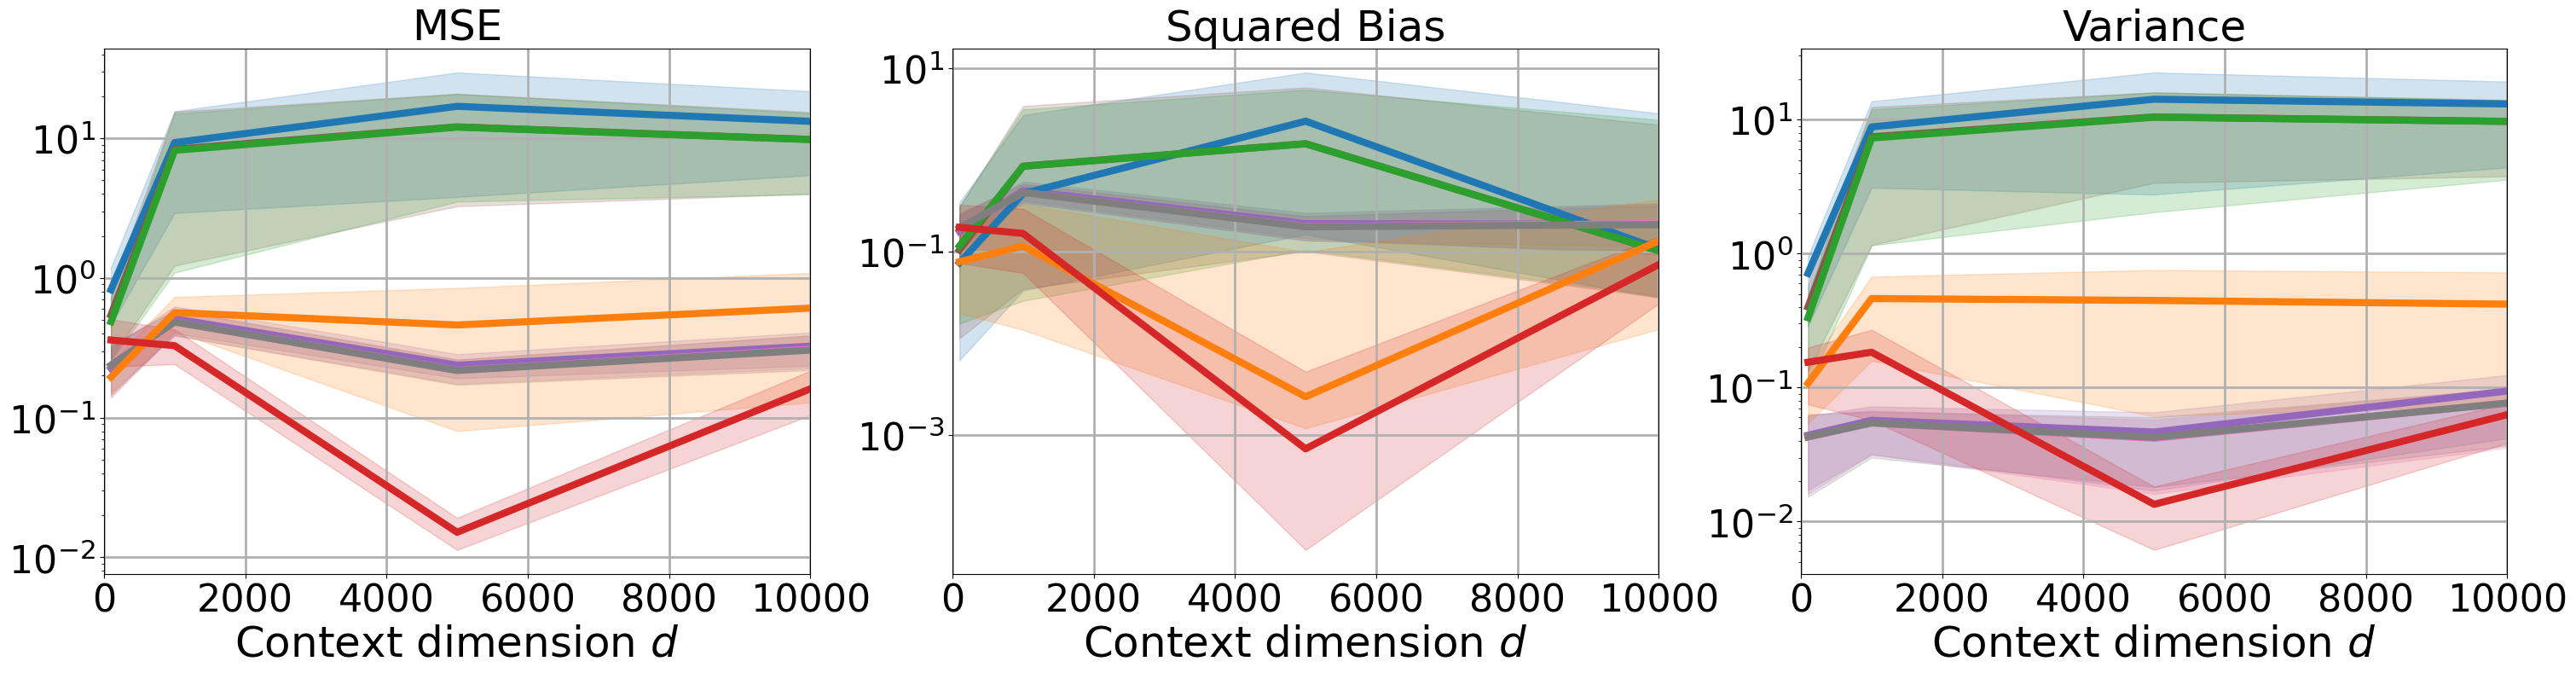
\includegraphics[width=1\textwidth]{figures/mr/mips_experiments/ope_vs_d_nac_250_alphatar_0_8_n_200.png}
	    \subcaption{$n_{a}=250$, $n = 200$, $\alpha^\ast = 0.8$}
	    \label{subfig:na-250-neval-200-alphatar-0-8-d-mips}
	\end{subfigure}
    \caption{MSE with varying context dimensions $d$ for different choices of parameters.}
    \label{fig:mse-vs-d-mips}
\end{figure}

\begin{figure}[h!]
    \centering
	\begin{subfigure}{0.8\textwidth}
	    \centering
	    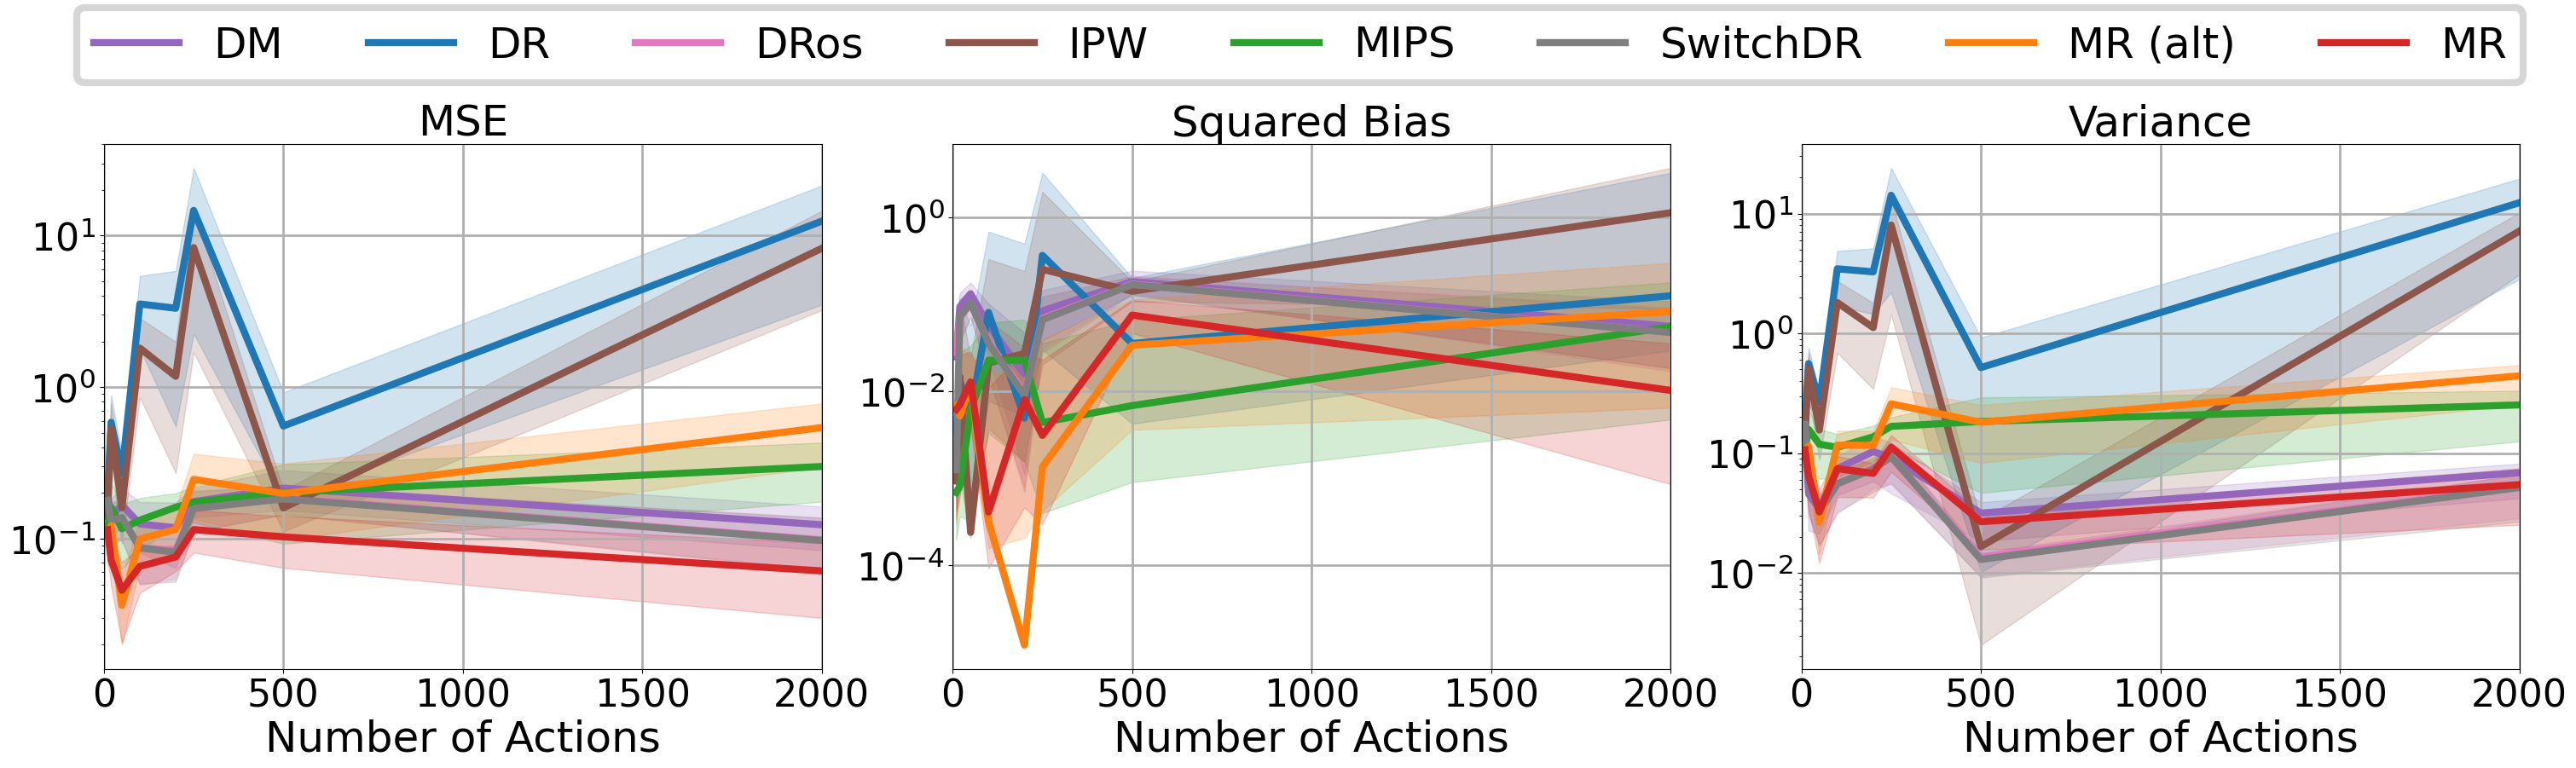
\includegraphics[width=1\textwidth]{figures/mr/mips_experiments/ope_vs_nac_dimc_1000_alphatar_0_4_neval_100_ntrain_100000.png}
	    \subcaption{$d=1000$, $n = 100$, $\alpha^\ast = 0.4$}
	    \label{subfig:d-1000-neval-100-alphatar-0-4-nac-mips}
	\end{subfigure}\\
	\begin{subfigure}{0.8\textwidth} 
	    \centering
	    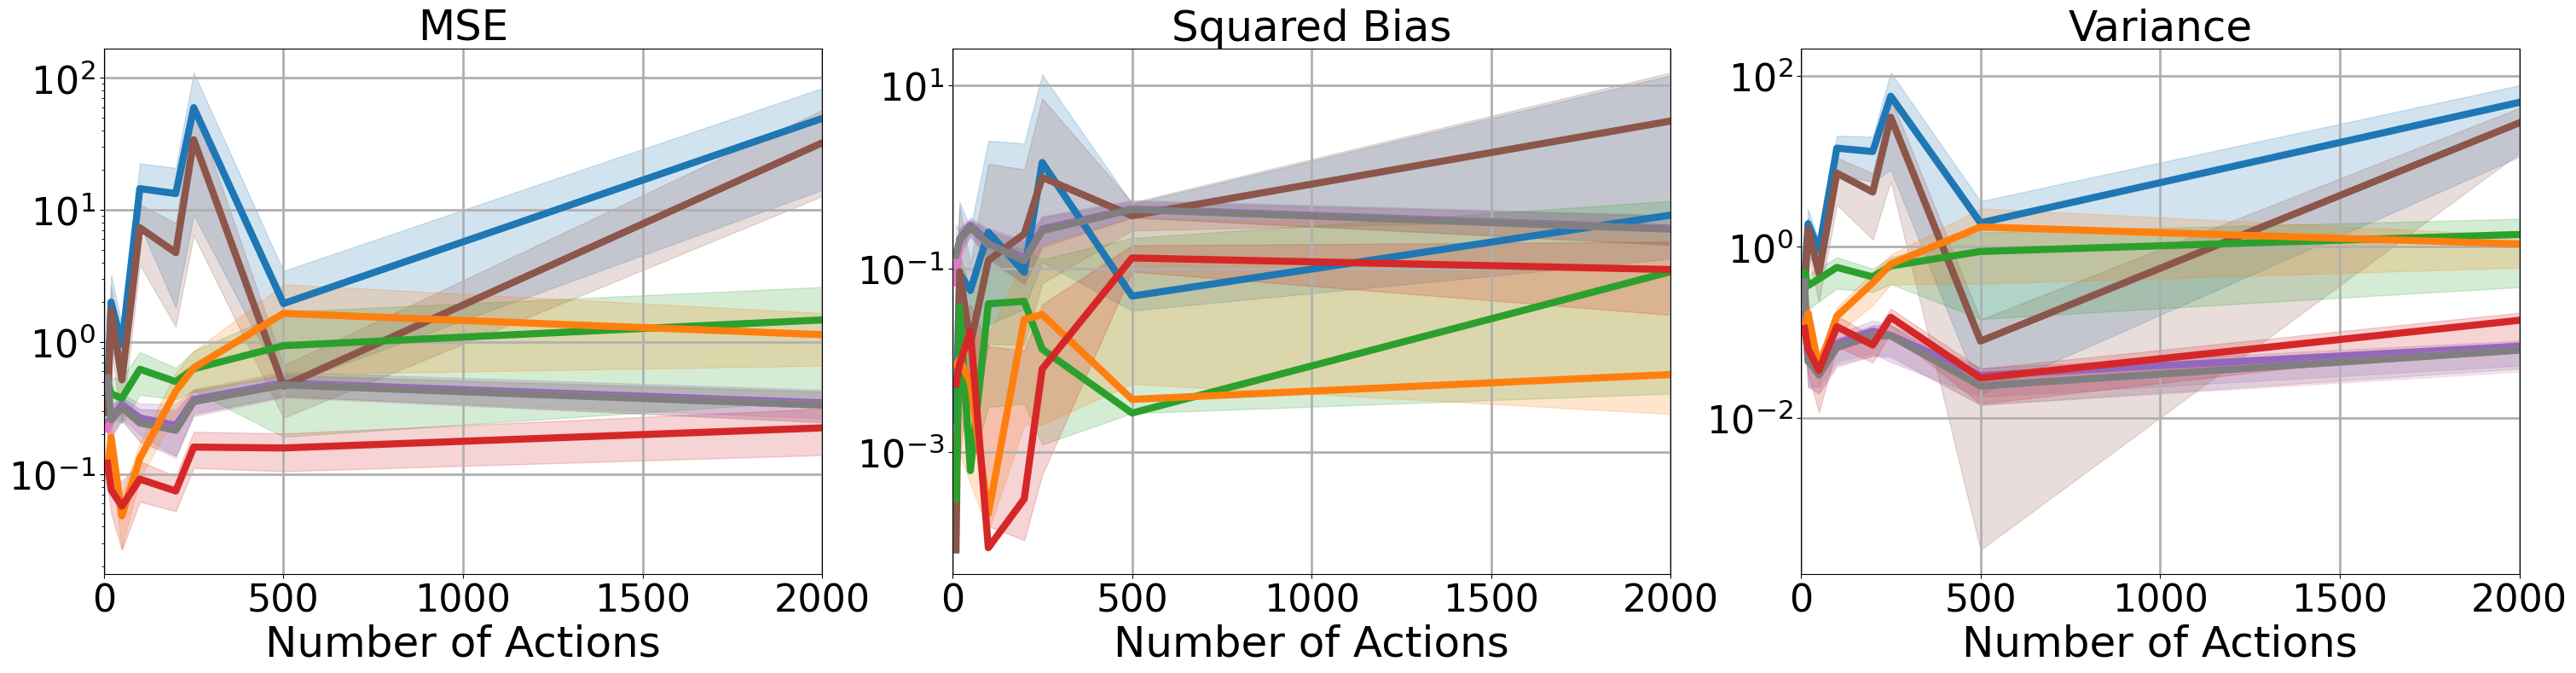
\includegraphics[width=1\textwidth]{figures/mr/mips_experiments/ope_vs_nac_dimc_1000_alphatar_0_8_neval_100_ntrain_100000.png}
	    \subcaption{$d=1000$, $n = 100$, $\alpha^\ast = 0.8$}
	    \label{subfig:d-1000-neval-100-alphatar-0-8-nac-mips}
	\end{subfigure}\\
	\begin{subfigure}{0.8\textwidth} 
	    \centering
	    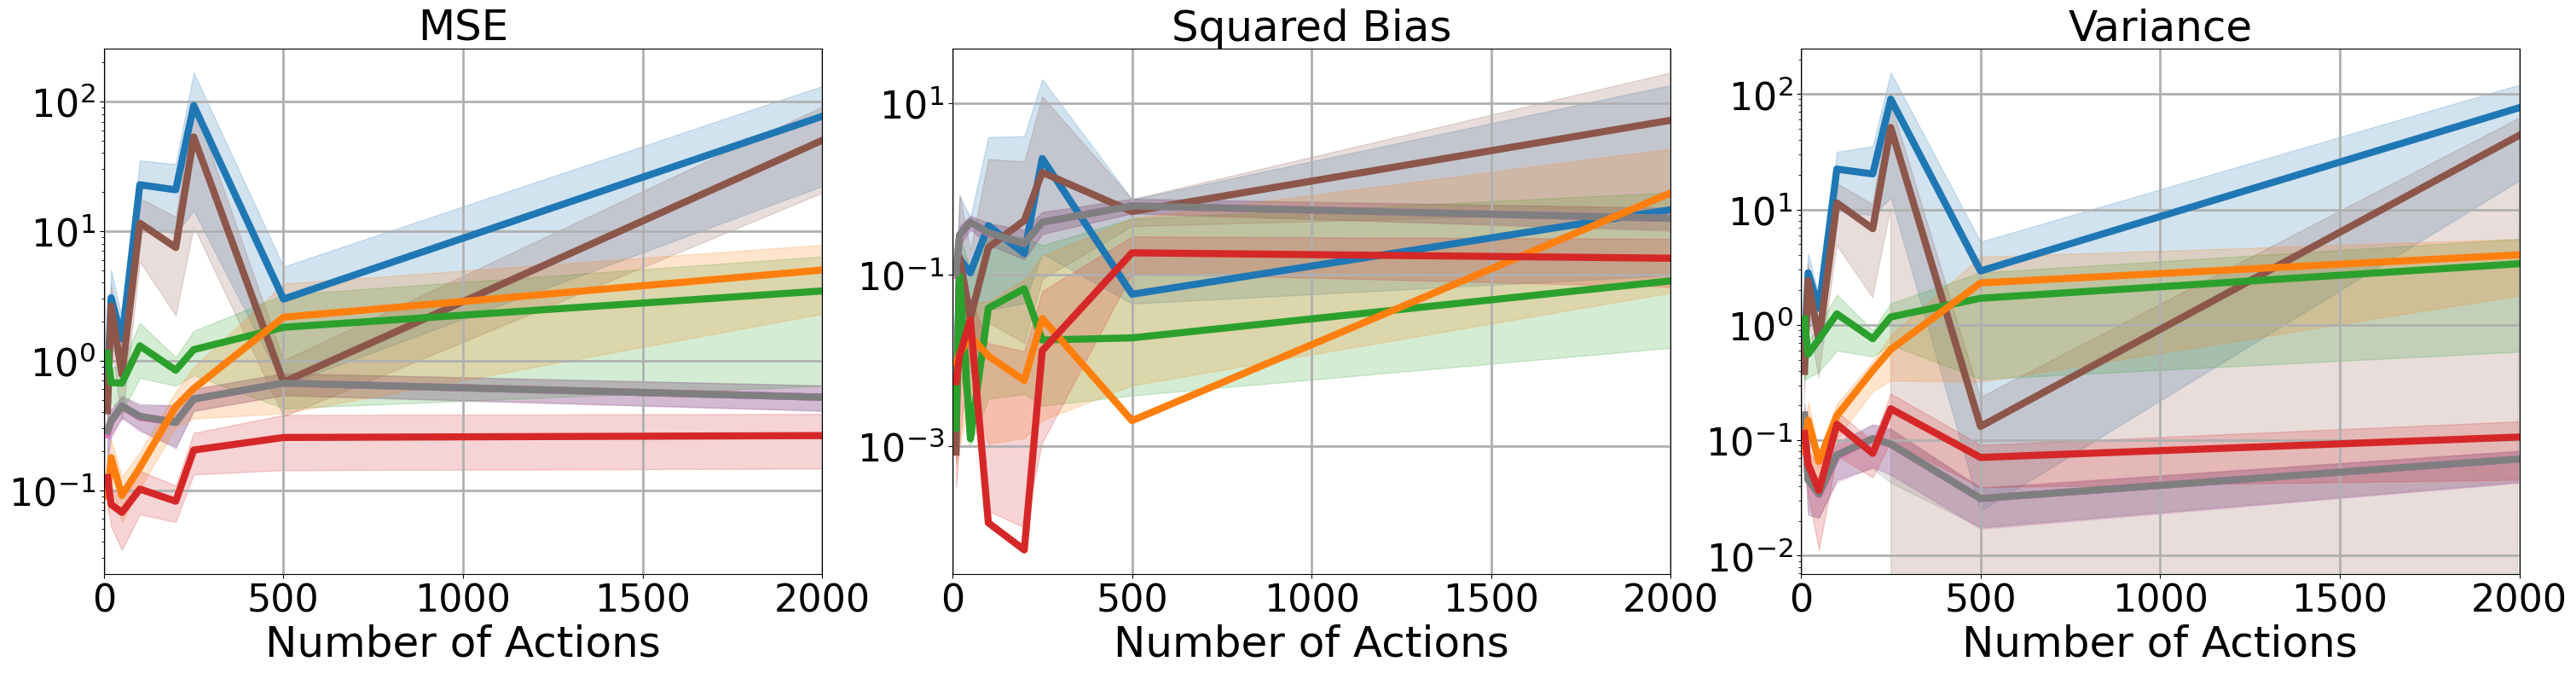
\includegraphics[width=1\textwidth]{figures/mr/mips_experiments/ope_vs_nac_dimc_1000_alphatar_1_0_neval_100_ntrain_100000.png}
	    \subcaption{$d=1000$, $n = 100$, $\alpha^\ast = 1.0$}
	    \label{subfig:d-1000-neval-100-alphatar-1-0-nac-mips}
	\end{subfigure}
    \caption{MSE with varying number of actions $n_a$ for different choices of parameters.}
    \label{fig:mse-vs-nac-mips}
\end{figure}

\begin{sidewaystable}[ht]
    \centering
        \caption{Mean-squared error results with 2 standard errors for synthetic data setup considered in Section \ref{sec:exp-synth} with $d=5000$, $n_a = 50$, $\alpha^\ast = 0.8$. We use a fixed budget of datapoints (denoted by $N$) for each baseline and in the case of MR we use $m=2000$ of the available datapoints to estimate $\hat{w}(y)$ and the rest of data to evaluate the MR estimator (i.e. $n = N-2000$ for MR). In contrast, for IPW and MIPS since the importance ratios are already known, we use all of the $N$ datapoints for evaluation of the off-policy value (i.e. $n=N$ for IPW and MIPS).}
    \label{tab:known_ratios}
    \begin{tiny}
    \begin{tabular}{l|llllll}
\toprule
& $N$ & 2800 & 3200 & 6400 & 10000 & 12000 \\
\midrule
\multirow{2}{*}{
\begin{tiny}
\textbf{GT weights $\rho(a, x)$ and estimated reward model $\hat{\mu}(a, x)$}
\end{tiny}}
& DM & 0.137$\pm$0.028 & 0.099$\pm$0.012 & 0.103$\pm$0.012 & 0.093$\pm$0.010 & 0.089$\pm$0.010 \\
\multirow{2}{*}{
\begin{tiny}
($m=2000$ used for training $\hat{\mu}(a, x)$ and $n=N-2000$ 
\end{tiny}}
& DR & 0.227$\pm$0.065 & 0.068$\pm$0.035 & 0.068$\pm$0.022 & \textbf{0.024$\pm$0.011} & 0.045$\pm$0.015 \\
\multirow{2}{*}{
\begin{tiny}
used for evaluation)
\end{tiny}} & DRos & 0.128$\pm$0.027 & 0.072$\pm$0.011 & 0.049$\pm$0.014 & 0.063$\pm$0.014 & 0.051$\pm$0.016 \\
& SwitchDR & 0.128$\pm$0.027 & 0.059$\pm$0.014 & 0.052$\pm$0.013 & 0.061$\pm$0.015 & 0.056$\pm$0.016 \\
\hline
\\
\multirow{2}{*}{
\begin{tiny}
\textbf{GT weights} (all of $N$ datapoints are used for evaluation)
\end{tiny}}
& IPW & 0.237$\pm$0.062 & 0.066$\pm$0.036 & 0.067$\pm$0.021 & 0.025$\pm$0.011 & \textbf{0.044$\pm$0.014} \\
& MIPS & 0.236$\pm$0.062 & 0.065$\pm$0.035 & 0.067$\pm$0.021 & 0.025$\pm$0.011 & \textbf{0.044$\pm$0.014} \\
\hline
\multirow{3}{*}{
\begin{tiny}
\textbf{Estimated weights $\hat{w}(y)$}
\end{tiny}}
\multirow{3}{*}{
\begin{tiny}
($m=2000$ used for training
\end{tiny}} \\
\multirow{3}{*}{
\begin{tiny}
and $n=N-2000$ used for evaluation)
\end{tiny}} 
& MR (Ours) & \textbf{0.045$\pm$0.015} & \textbf{0.042$\pm$0.014} & \textbf{0.048$\pm$0.020} & 0.049$\pm$0.020 & 0.047$\pm$0.016
\\
\\
\bottomrule
\end{tabular}
    \end{tiny}
\end{sidewaystable}
\subsubsection{Known policy ratios $\rho(a, x)$}
Our previous setting of unknown importance policy ratios $\rho(a, x)$ captures a wide variety of real-world applications, ranging from health care to autonomous driving. In addition, to demonstrate the utility of MR in settings with known $\rho(a, x), p(e\mid a, x)$ and unknown $w(y)$ (for our proposed method, MR), we have conducted additional experiments. Here, we use a fixed budget of datapoints (denoted by $N$) for each baseline and for MR we allocate $m=2000$ of the available datapoints to estimate $\hat{w}(y)$ and use the remaining for evaluating the MR estimator (i.e., $n=N-2000$ for MR). In contrast, for IPW and MIPS (since the importance ratios are already known), we use all of the $N$ datapoints to evaluate the off-policy value (i.e. $n=N$ for IPW and MIPS).

The results included in Table \ref{tab:known_ratios} show that MR achieves the smallest MSE among the baselines for $N\leq 6400$. However, we observe that the MSE of IPW, DR and MIPS (with true importance weights) falls below that of MR (with estimated weights $\hat{w}$) when the data size $N$ is large enough (i.e., $N\geq 10,000$). This is to be expected since IPW, DR and MIPS are unbiased (i.e., use ground truth importance ratios $\rho(a, x)$) whereas MR uses estimated weights $\hat{w}(y)$ (and hence may be biased). MR still performs the best when $N\leq 6400$.

\subsection{Experiments on classification datasets}\label{subsec:additional-experiments-classification}
Here, we conduct experiments on four classification datasets, OptDigits, PenDigits, SatImage and Letter datasets from the UCI repository \citep{dua2019uci}, the Digits dataset from scikit-learn library, as well as the Mnist \citep{deng2012mnist} and CIFAR-100 datasets \citep{krizhevsky2009learning}.

\paragraph{Setup}
Following previous works \citep{dudik2014doubly, kallus2021optimal, mehrdad2018more,wang2017optimal}, the classification datasets are transformed to contextual bandit feedback data. The classification dataset comprises $\{x_i, a^\gt_i\}_{i=1}^{n_0}$, where $x_i\in \Xspace$ are feature vectors and $a^\gt_i\in \Aspace$ are the ground-truth labels. In the contextual bandits setup, the feature vectors $x_i$ are considered to be the contexts, whereas the actions correspond to the possible class of labels. We split the dataset into training and testing datasets of sizes $m$ and $n$ respectively. We present the results for a range of different values of $m$ and $n$.

\paragraph{Reward function}
Let $X$ be a context with ground truth label $A^\gt$, we define the reward for action $A$ as:
\[
Y \coloneqq \ind(A = A^\gt).
\]

\paragraph{Behaviour and target policies}
Using the $m$ training datapoints, we first train a classifier $f: \Xspace\rightarrow \mathbb{R}^{|\Aspace|}$ which takes as input the feature vectors $x_i$ and outputs a vector of softmax probabilities over labels, i.e. the $a$-th component of the vector $f(x)$, denoted as $(f(x))_{a}$ corresponds to the estimated probability $\p(A^{\gt} = a \mid X=x)$.

Next, we use $f$ to define the ground truth behaviour policy, 
\[
\beh(a\mid x) = (f(x))_{a}.
\]
For the target policies, we use $f$ to define a parametric class of target policies using a trained classifier $f: \Xspace\rightarrow \mathbb{R}^{|\Aspace|}$. 
\[
\pi^{\alpha^\ast}(a\mid x) =\alpha^\ast\cdot \ind(a= \arg\max_{a' \in \Aspace} (f(x))_{a'}) +  \frac{1-\alpha^\ast}{|\Aspace|},
\]
where $\alpha^\ast \in [0, 1]$. A value of $\alpha^\ast$ close to 1 leads to a near-deterministic and well-performing policy. As $\alpha^\ast$ decreases, the policy gets increasingly worse and `noisy'. In this experiment, we consider target policies $\tar = \pi^{\alpha^\ast}$ for $\alpha^\ast \in \{0.0, 0.2, 0.4, \dots, 1.0\}$. 

Using the behaviour policy defined above, we generate the contextual bandits data described with training and evaluation datasets of sizes $m$ and $n$ respectively.

\paragraph{Estimation of behaviour policy $\hatbeh$ and marginal ratio $\hat{w}(y)$}
We do not assume that the behaviour policy $\beh$ is known, and therefore estimate it using training data. To estimate the behaviour policy $\hatbeh$, we train a random forest classifier using the training data. This estimate of behaviour policy is used for all the baselines in our experiment. 
Since the reward is binary, we can estimate the marginal ratios $\hat{w}(y) = \Ebeh[\hat{\rho}(A, X)\mid Y=y]$ by directly estimating the sample mean of $\hat{\rho}(A, X)$ for datapoints with $Y=y$. We re-use the $m$ training datapoints to estimate this sample mean. 

\paragraph{Baselines}
We compare our estimator with Direct Method (DM), IPW and DR estimators. 
In addition, we also consider Switch-DR \citep{wang2017optimal} and DR with Optimistic Shrinkage (DRos) \citep{su2020doubly}.
To estimate $\hat{q}(x, a)$ for DM and DR estimators, we use random forest classifiers (since reward $Y$ is binary). Moreover, because of the binary nature of $Y$, the alternative method of estimating MR yields the same estimator as the original method, therefore we do not consider the two separately here. Additionally, in this experiment, we do not include MIPS (or G-MIPS) baseline, as there is no natural informative embedding $E$ of the action $A$. 

\subsubsection{Results}
For this experiment, we compute the results over 10 different sets of logged data replicated with different seeds.
Figures \ref{fig:optdigits} - \ref{fig:cifar100} show the results corresponding to each baseline for the different datasets. It can be seen that across all datasets, the MR achieves the smallest MSE with increasing evaluation data size $n$. Moreover, across all datasets, MR attains the minimum MSE with relatively small number of evaluation data ($n\leq 100$).
% Moreover, the performance of the MR estimator improves significantly with increasing $n$, whereas there is little relative improvement in the performance of other baselines as $n$ increases. 
% In each of these experiments, we use the remaining dataset as the training data, i.e.\,

Unlike the experiments in Section \ref{sec:exp-synth}, we observe that the KL-divergence between target and behaviour policy decreases as $\alpha^\ast$ increases (see Figure \ref{fig:kl_div_multiclass}). 
Therefore, as $\alpha^\ast$ increases the shift between target and behaviour policies decreases.
Figures \ref{fig:optdigits} - \ref{fig:digits} show that as $\alpha^\ast$ increases, 
the difference between the MSE, squared bias and variance of MR and the other baselines decreases. This confirms our findings from earlier experiments that MR performs especially better than the other baselines when the difference between behaviour and target policies is large.

Moreover, the figures also include results with increasing number of training data $m$. It can be seen that MR out-performs the baselines even when the number of training data $m$ is small ($m = 100$). Moreover, the relative advantage of MR improves with increasing $m$.

\begin{figure}[t]
    \centering
    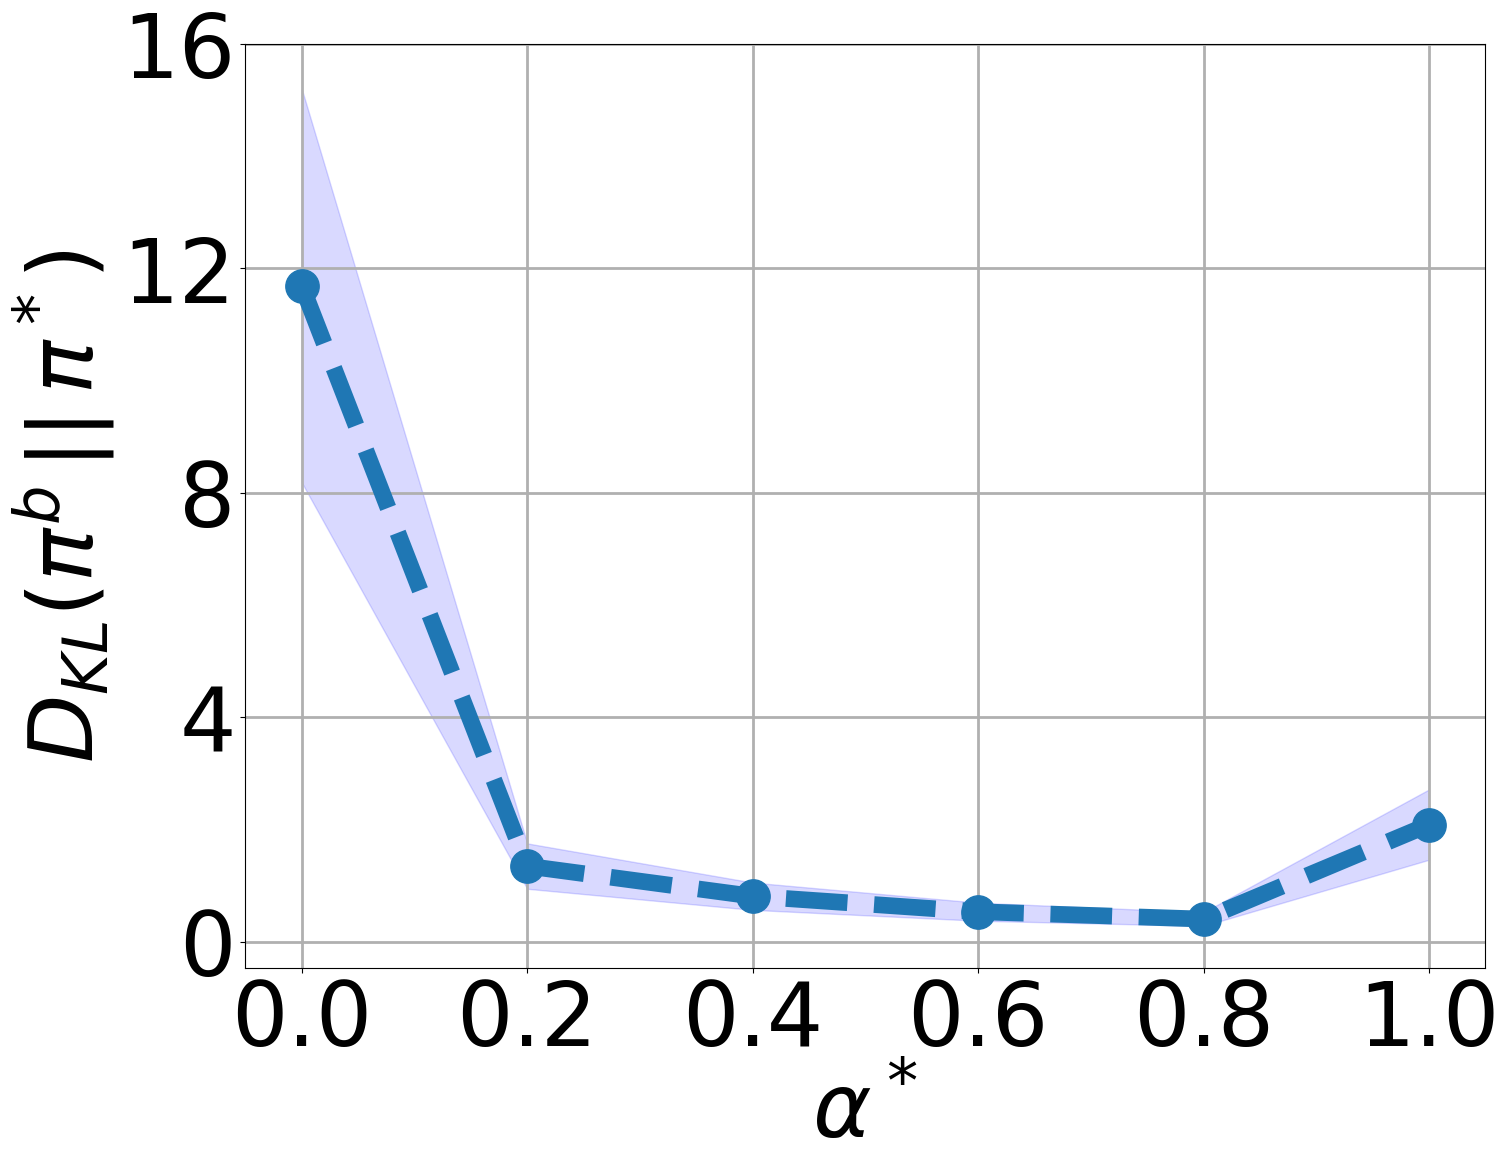
\includegraphics[width=0.3\textwidth]{figures/mr/kl-divergence-multiclass_w_uncertainty.png}
    \caption{KL divergence $D_{\textup{KL}}(\beh \, || \, \tar)$ with increasing $\alpha^\ast$ for the classification data experiments. Here, we only include the results for a specific choice of parameters for the Letter dataset. We observe similar results for other datasets and parameter choices.}
    \label{fig:kl_div_multiclass}
\end{figure}

\begin{figure}[ht]
    \centering
	\begin{subfigure}{0.8\textwidth}
	    \centering
	    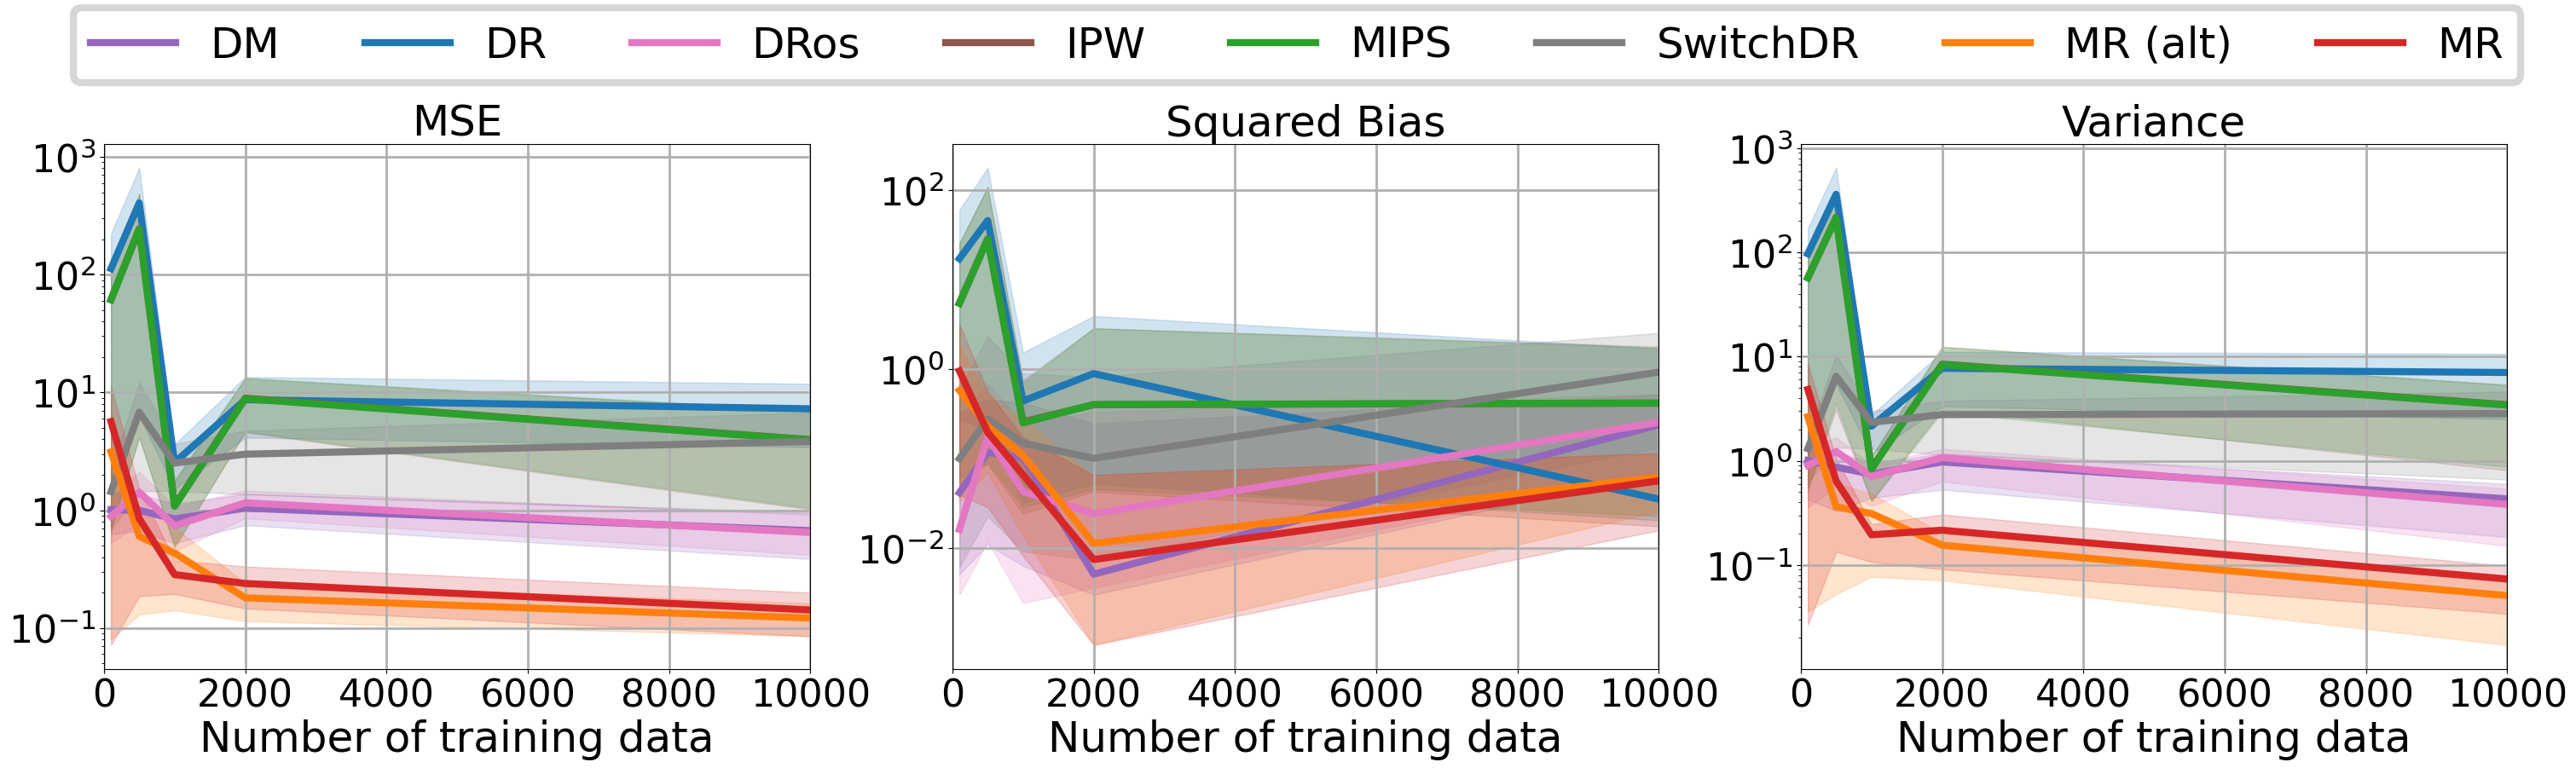
\includegraphics[width=1\textwidth]{figures/mr/mips_experiments/ope_vs_ntrain_dimc_1000_alphatar_0_8_nac_10_nev_10.png}
	    \subcaption{$d=1000$, $n = 10$, $\alpha^\ast = 0.8$}
	    \label{subfig:d-1000-neval-10-alphatar-0-8-ntr-mips}
	\end{subfigure}\\
	\begin{subfigure}{0.8\textwidth} 
	    \centering
	    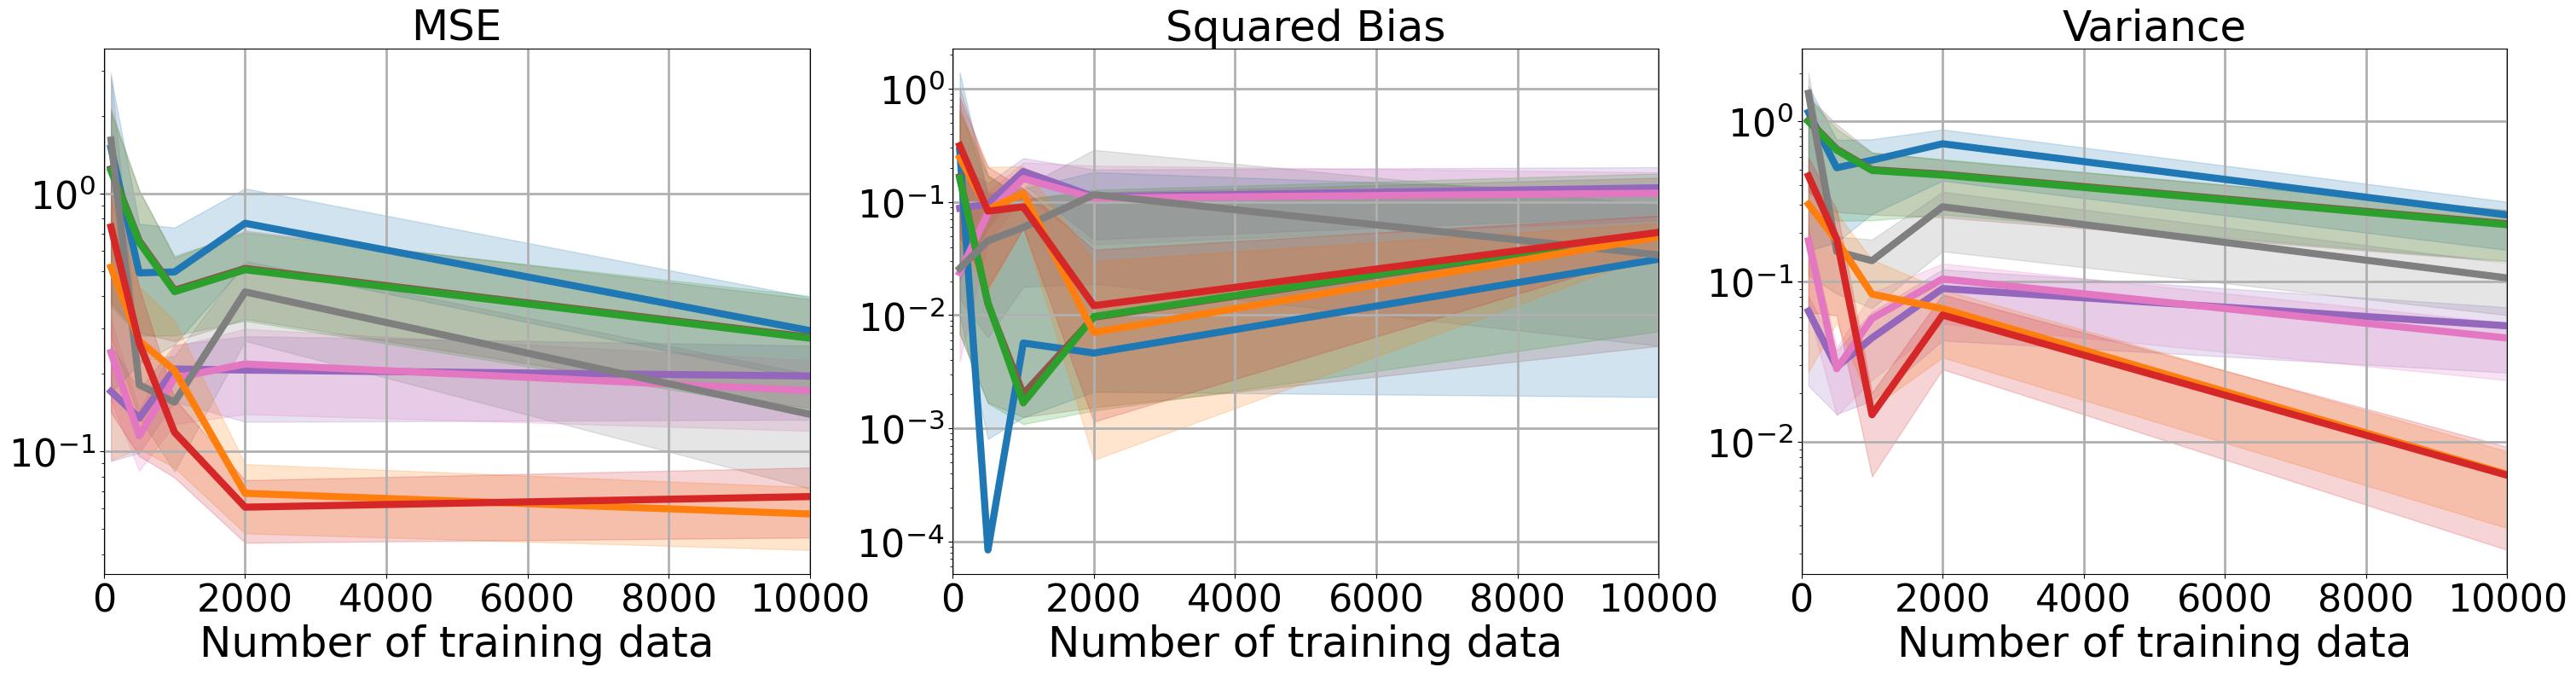
\includegraphics[width=1\textwidth]{figures/mr/mips_experiments/ope_vs_ntrain_dimc_1000_alphatar_0_8_nac_10_nev_200.png}
	    \subcaption{$d=1000$, $n = 200$, $\alpha^\ast = 0.8$}
	    \label{subfig:d-1000-neval-200-alphatar-0-8-ntr-mips}
	\end{subfigure}\\
	\begin{subfigure}{0.8\textwidth} 
	    \centering
	    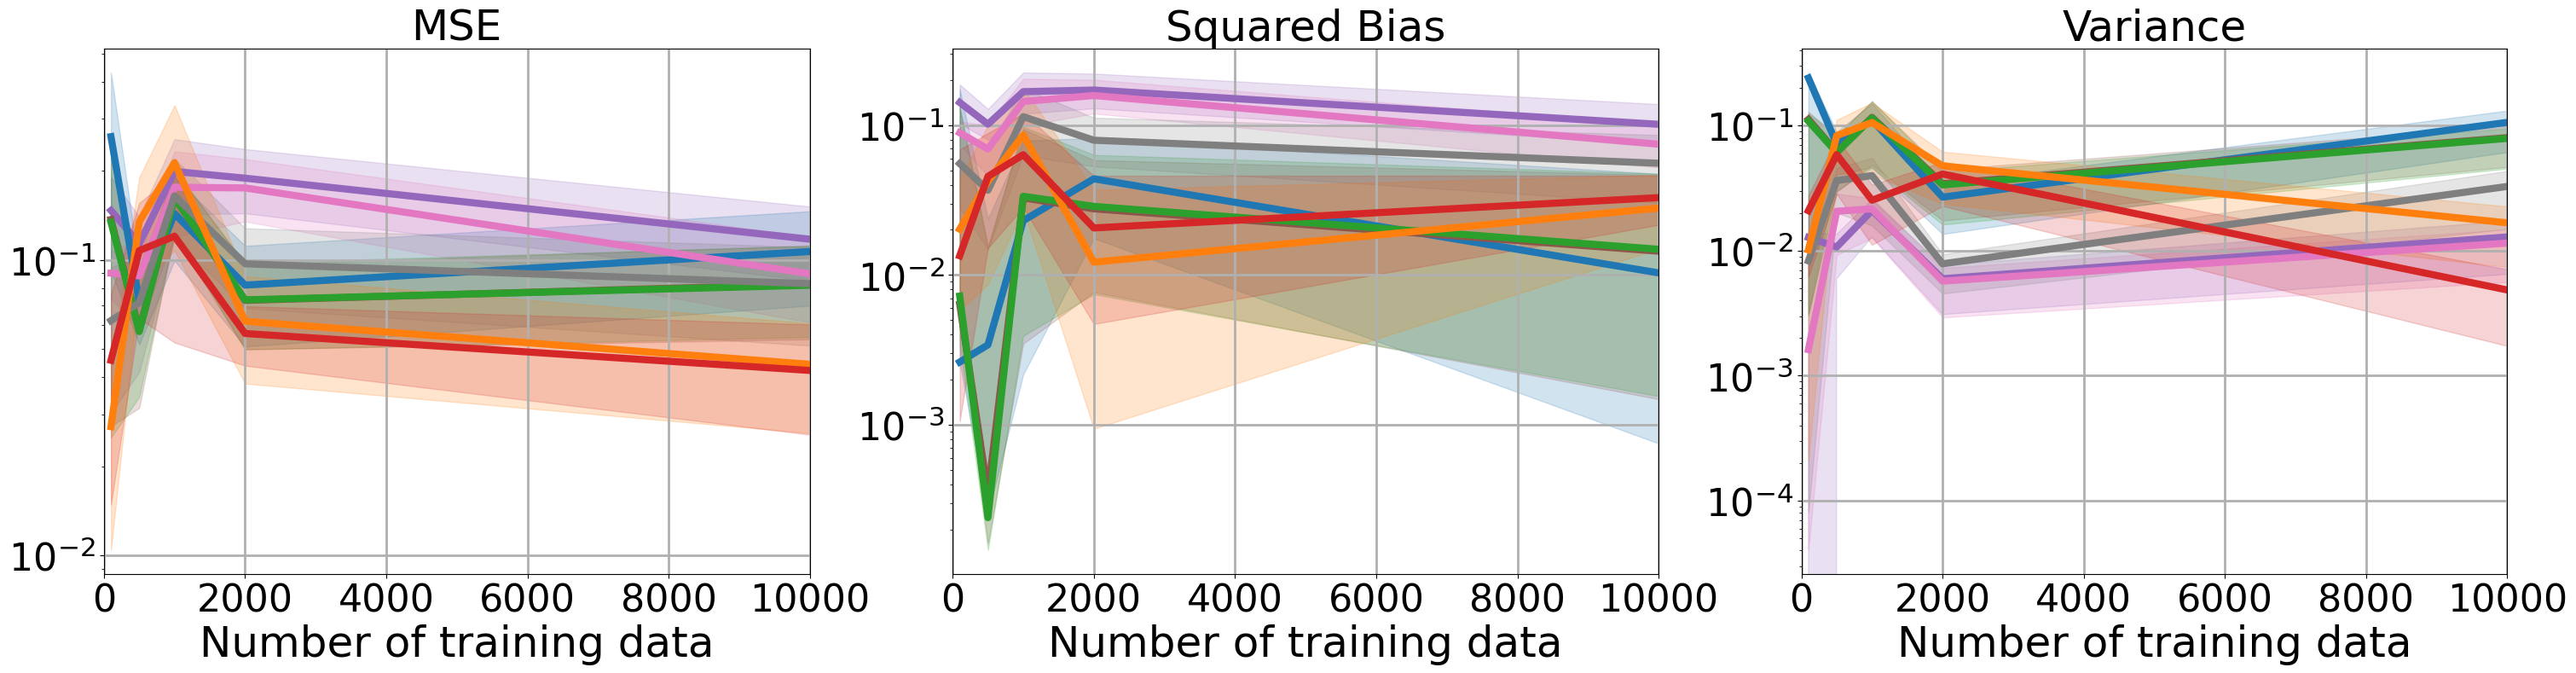
\includegraphics[width=1\textwidth]{figures/mr/mips_experiments/ope_vs_ntrain_dimc_1000_alphatar_0_8_nac_10_nev_800.png}
	    \subcaption{$d=1000$, $n = 800$, $\alpha^\ast = 0.8$}
	    \label{subfig:d-1000-neval-800-alphatar-0-8-ntr-mips}
	\end{subfigure}
    \caption{MSE with varying number of training data $m$ for different choices of parameters.}
    \label{fig:mse-vs-ntr-mips}
\end{figure}

\begin{figure}[h!]
    \centering
	\begin{subfigure}{0.8\textwidth}
	    \centering
	    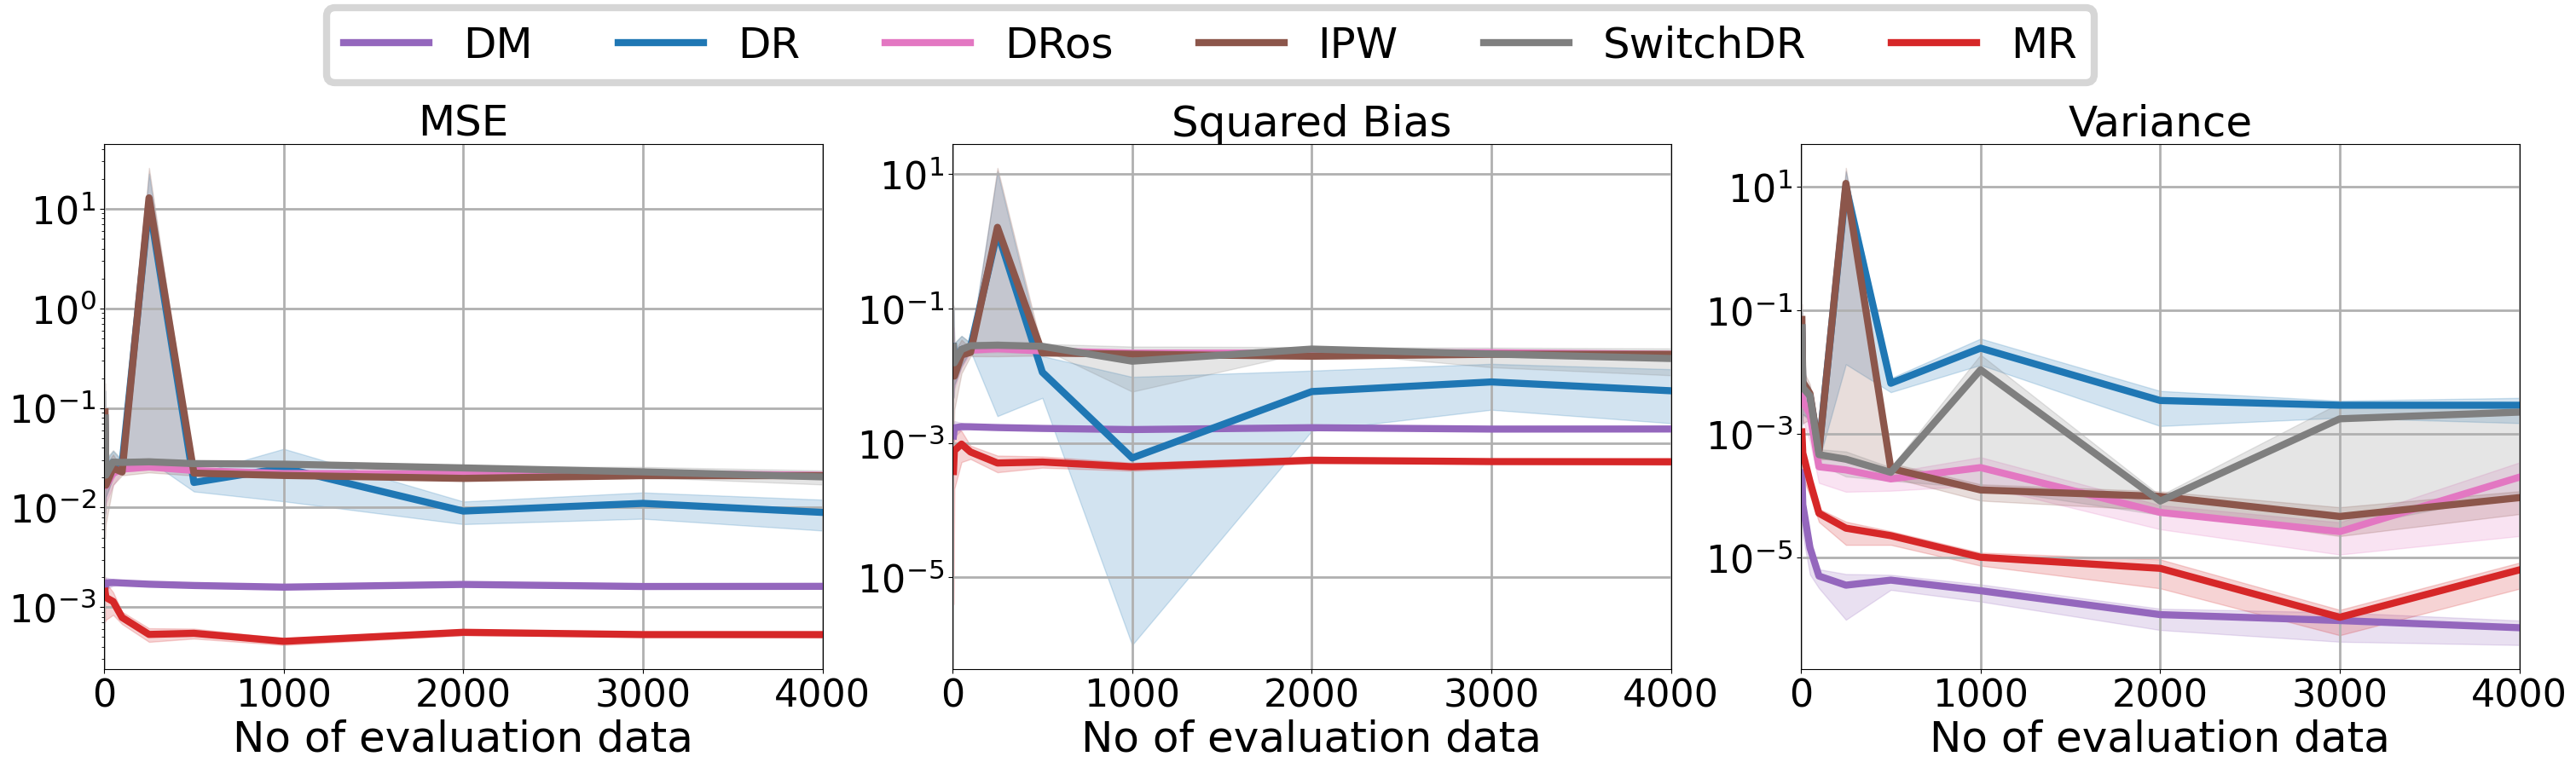
\includegraphics[width=1\textwidth]{figures/mr/multiclass/ope_vs_n_alphatar_0_2_optdigits_ntr1000.png}
	    \subcaption{Results with varying $n$ for $\alpha^\ast = 0.2$ and $m=1000$}
	    \label{subfig:opt-neval}
	\end{subfigure}\\
	\begin{subfigure}{0.8\textwidth} 
	    \centering
	    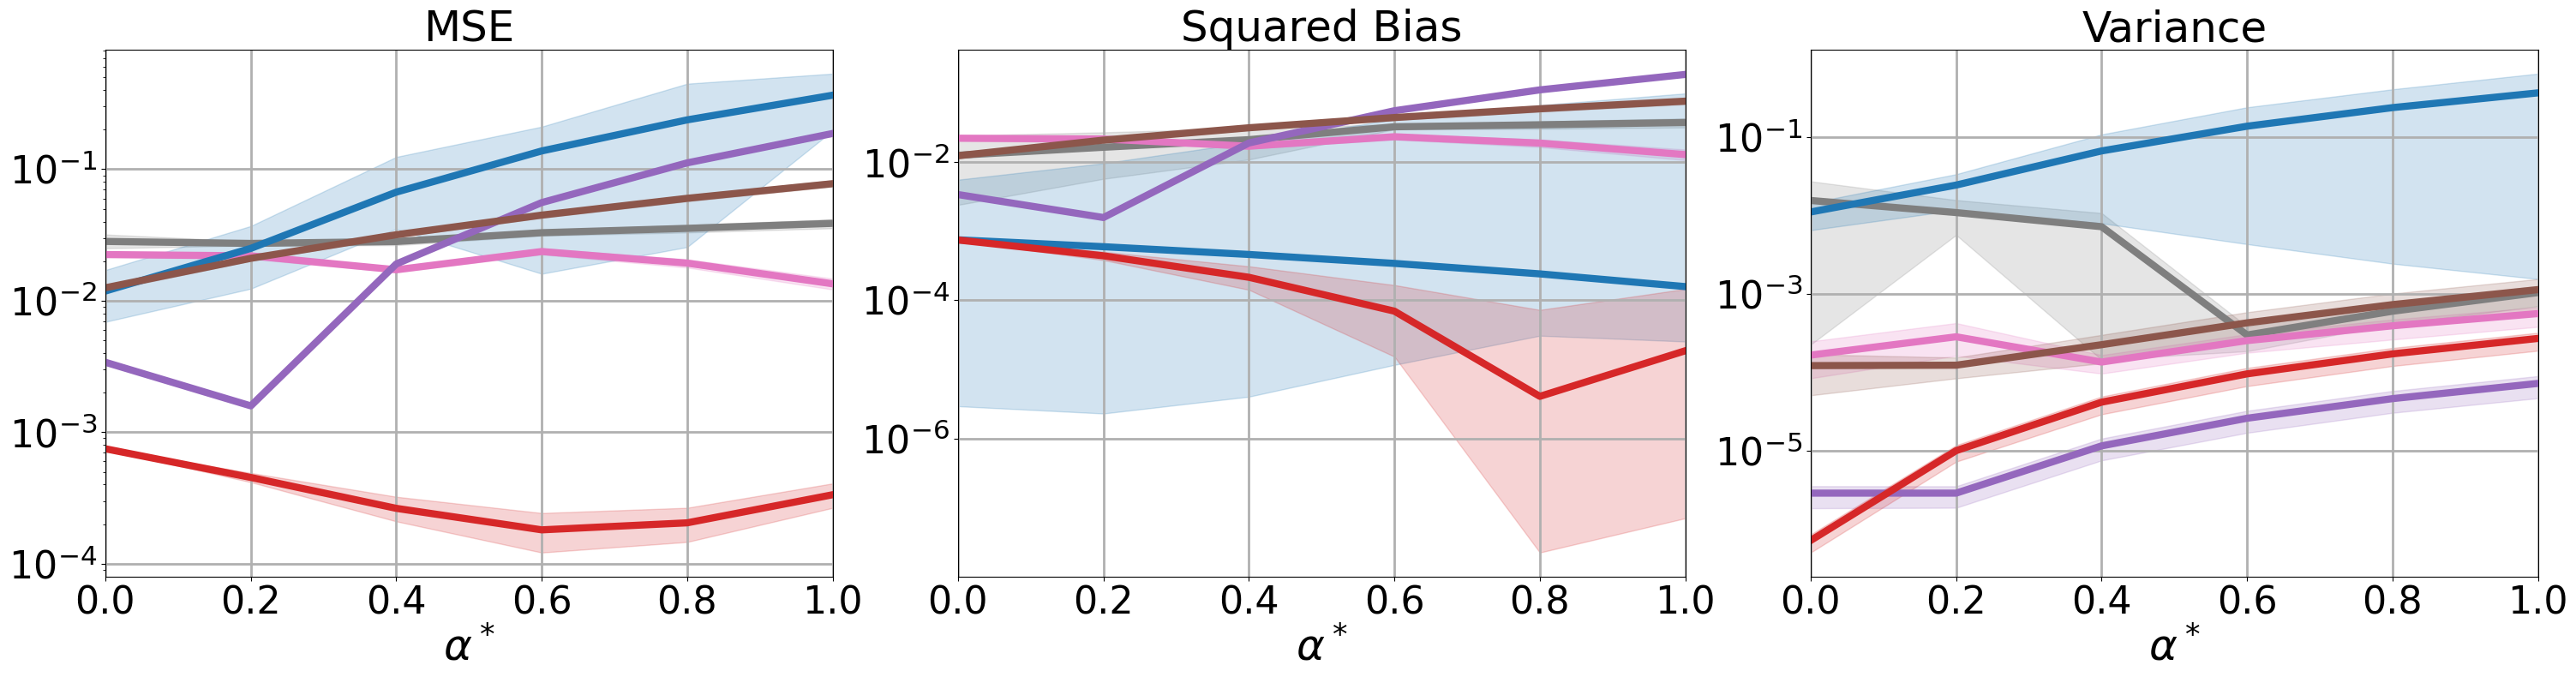
\includegraphics[width=1\textwidth]{figures/mr/multiclass/ope_vs_alphatar_neval_1000_optdigits_ntr_1000.png}
	    \subcaption{Results with varying $\alpha^\ast$ for $m = n = 1000$}
	    \label{subfig:opt-ae}
	\end{subfigure}\\
    \begin{subfigure}{0.8\textwidth} 
	    \centering
	    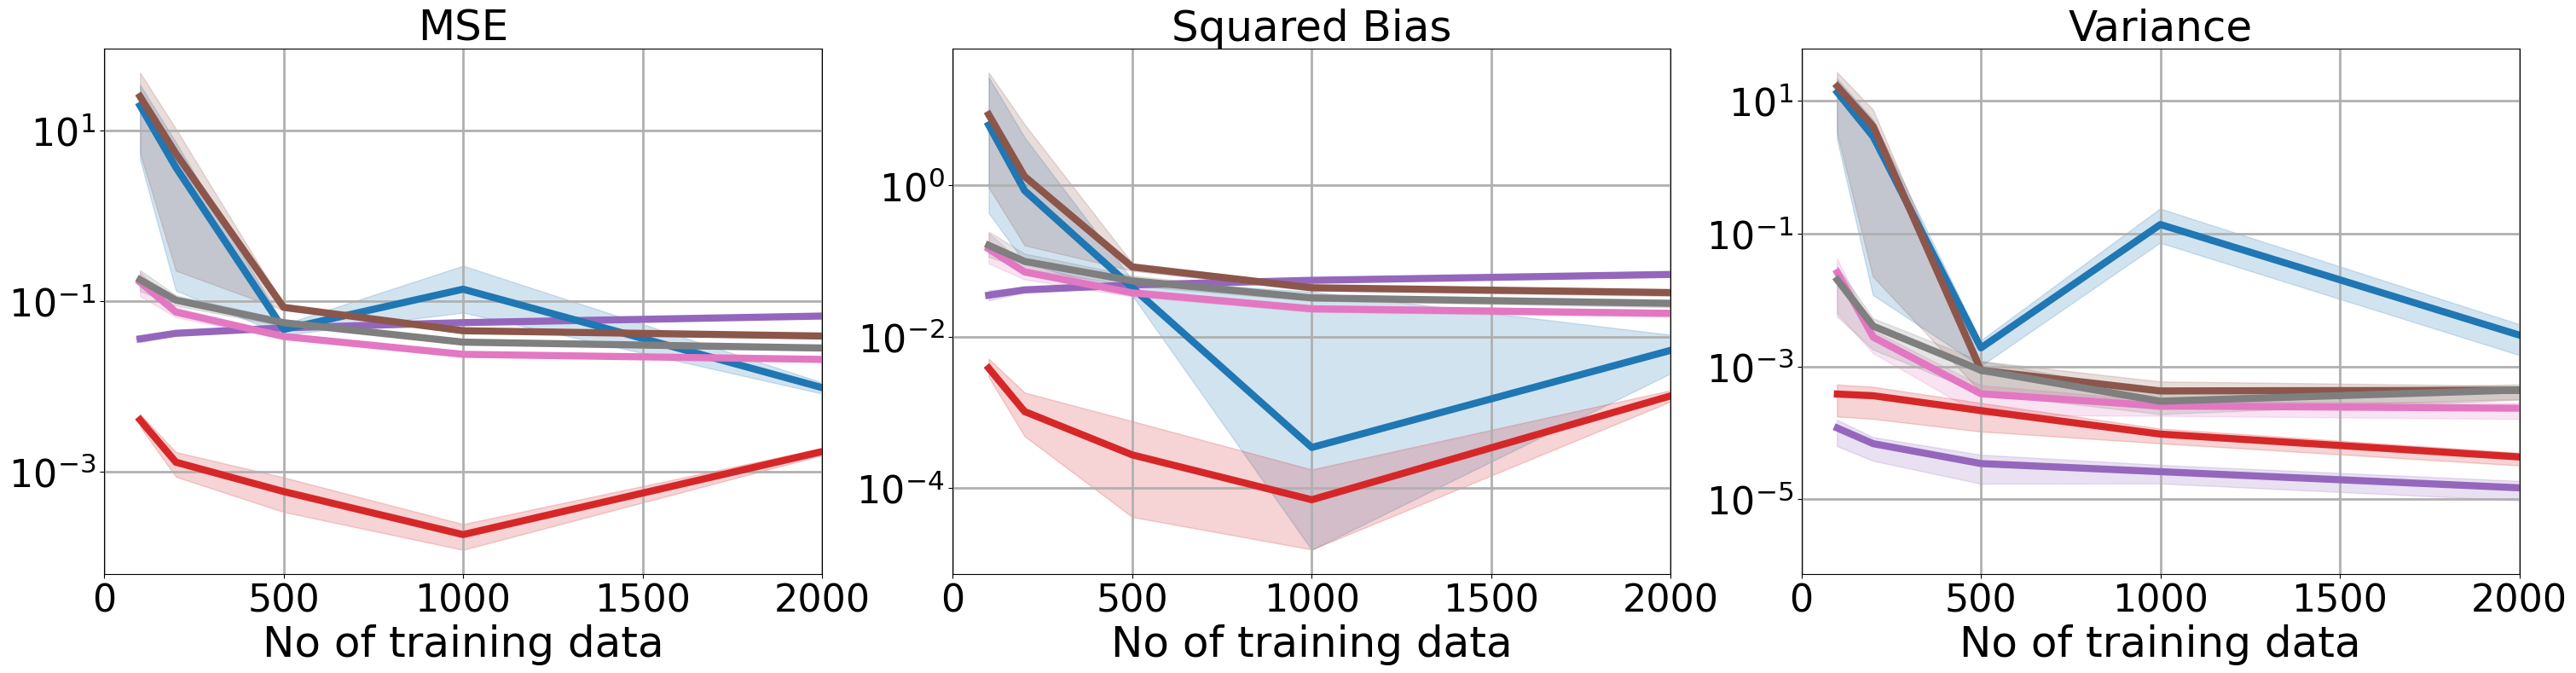
\includegraphics[width=1\textwidth]{figures/mr/multiclass/ope_vs_ntr_neval_1000_optdigits_alpha_0_6.png}
	    \subcaption{Results with varying $m$ for $n = 1000$ and $\alpha^\ast = 0.6$}
	    \label{subfig:opt-ntr}
	\end{subfigure}\\
	% \begin{subfigure}{1\textwidth} 
	%     \centering
	%     \includegraphics[width=6in]{figures/mr/optdigits_ab_neval_500_ae_0_0.png}
	%     \subcaption{Results with varying $\alpha^\ast$ for $n = 500$, $\alpha^b = 0.8$}
	%     \label{subfig:opt-ae}
	% \end{subfigure}
    \caption{Results for OptDigits dataset}
    \label{fig:optdigits}
\end{figure}

\begin{figure}[h!]
    \centering
	\begin{subfigure}{0.8\textwidth}
	    \centering
	    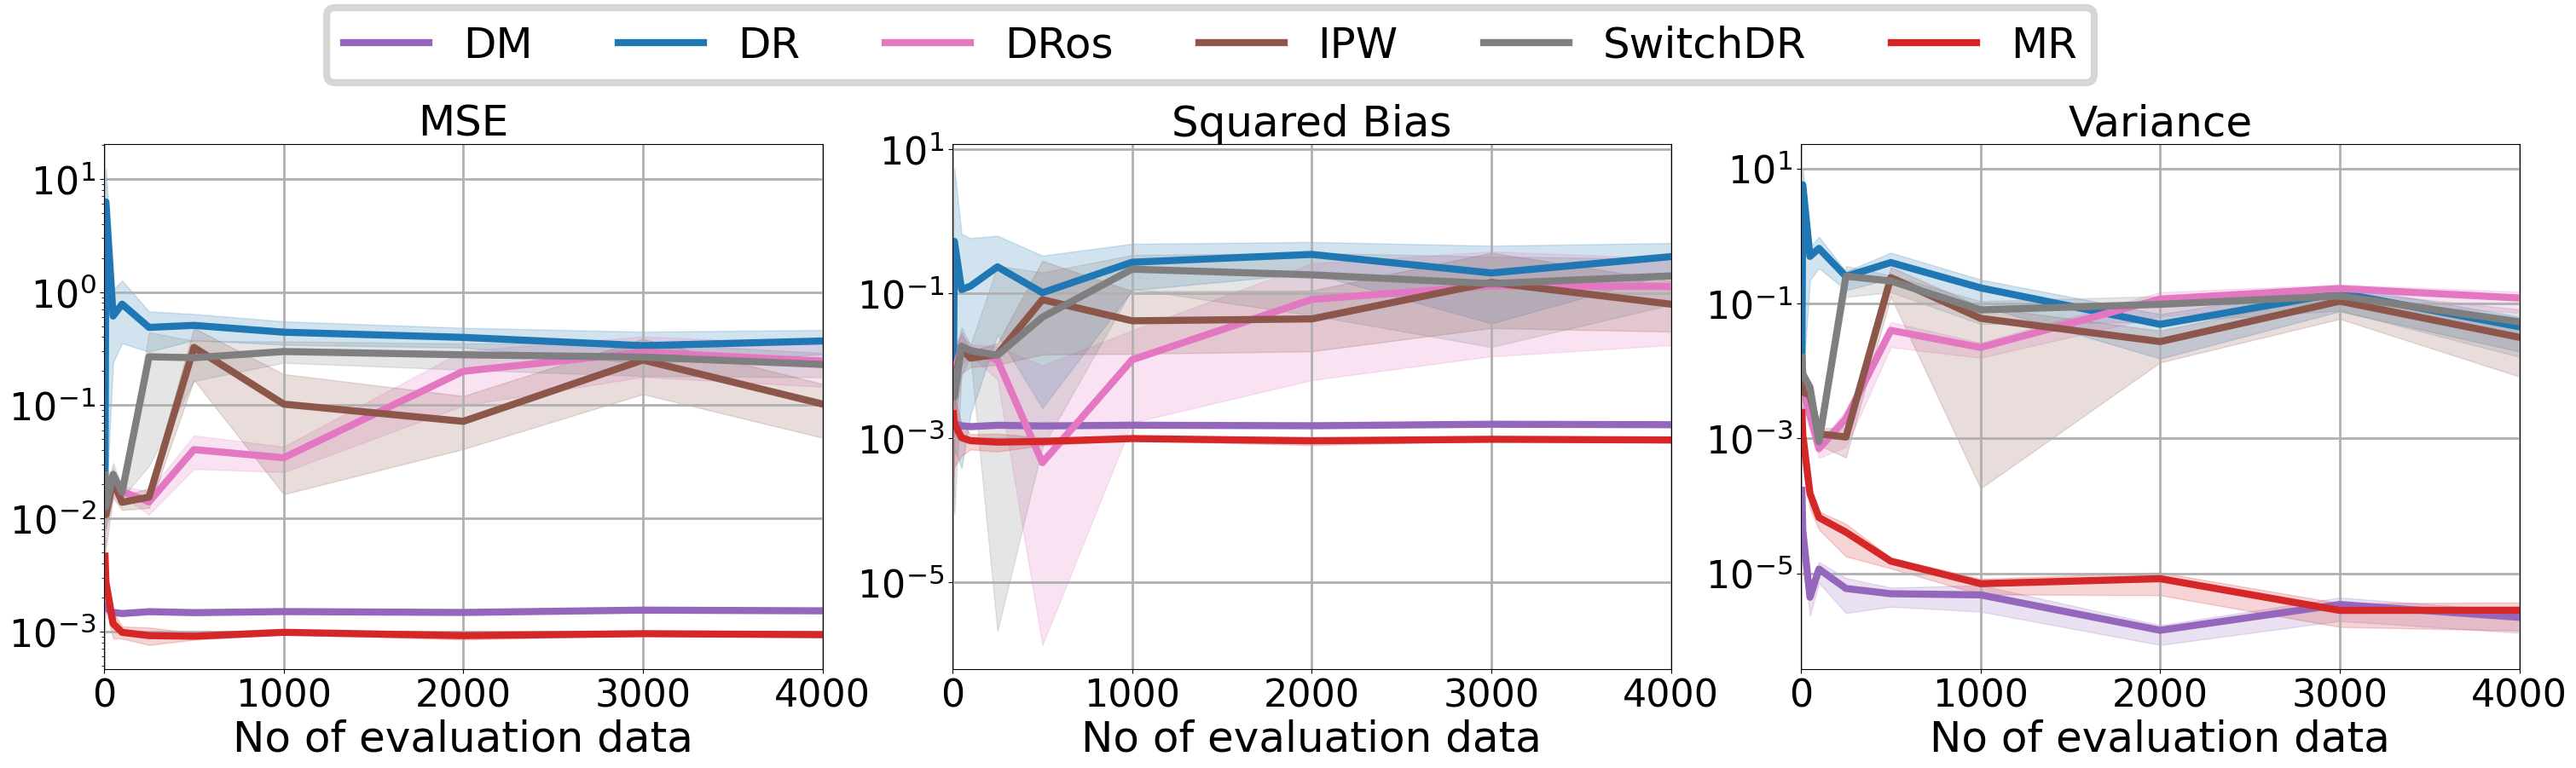
\includegraphics[width=1\textwidth]{figures/mr/multiclass/ope_vs_n_alphatar_0_2_pendigits_ntr1000.png}
	    \subcaption{Results with varying $n$ for $\alpha^\ast = 0.2$ and $m=1000$}
	    \label{subfig:pen-neval}
	\end{subfigure}\\
	\begin{subfigure}{0.8\textwidth} 
	    \centering
	    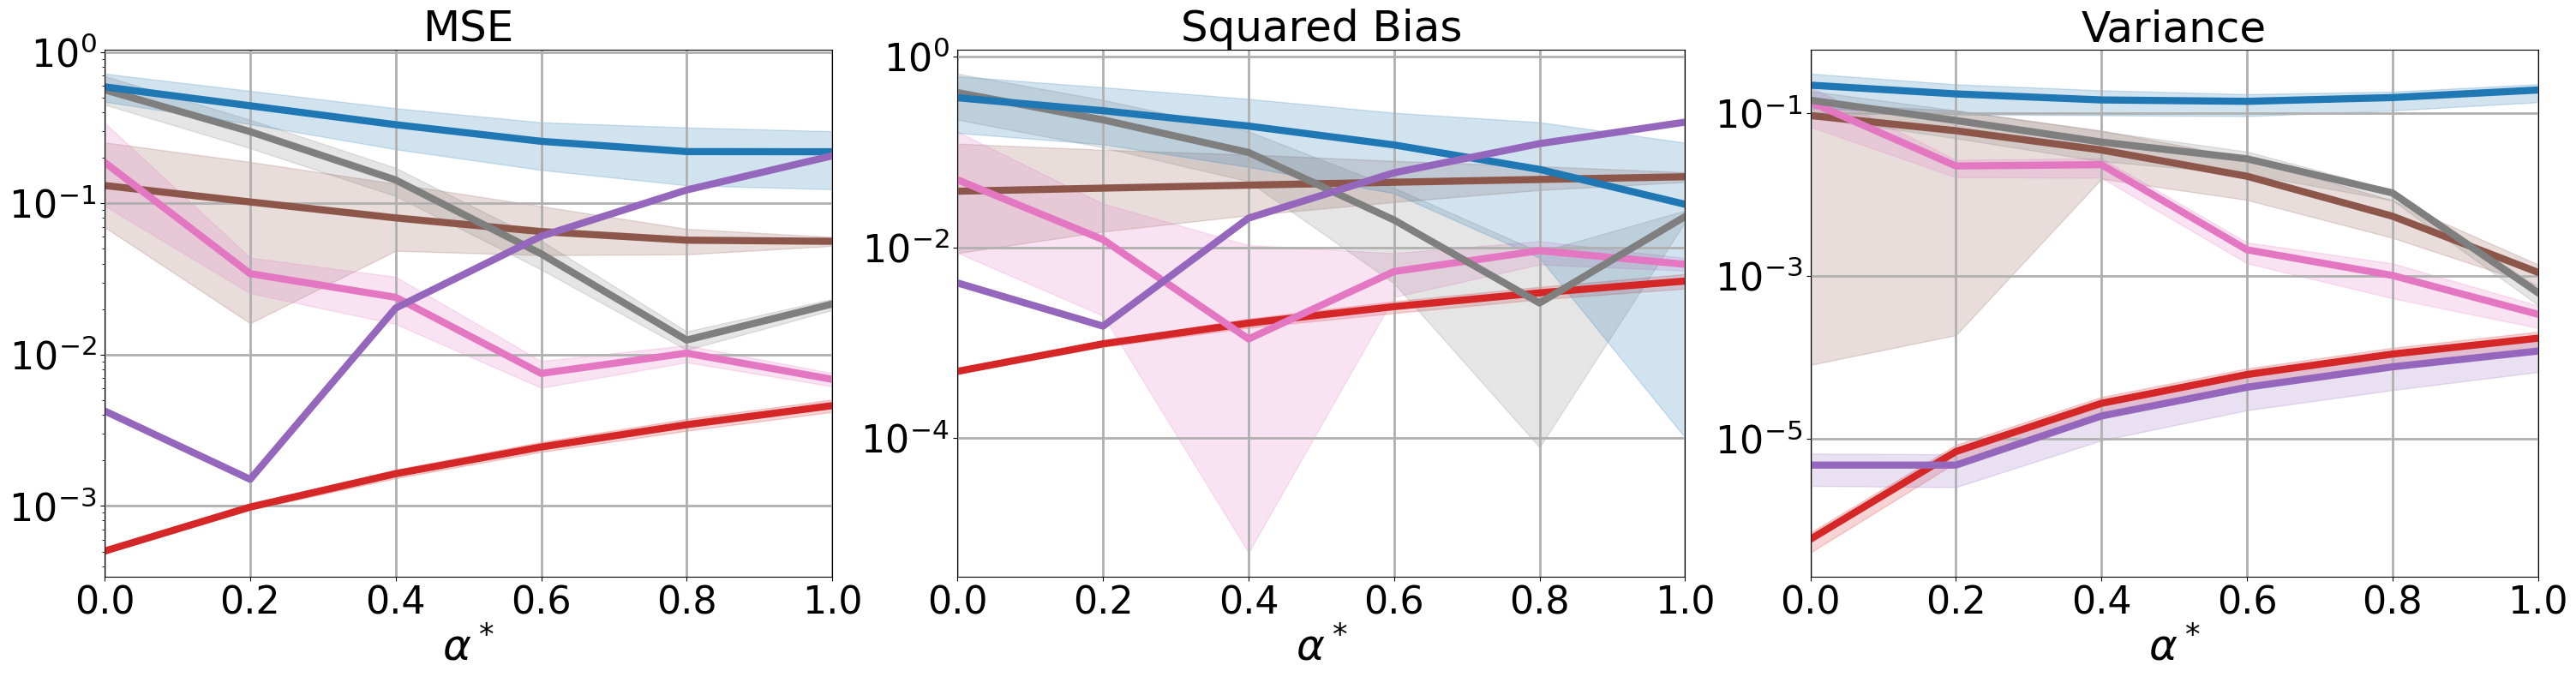
\includegraphics[width=1\textwidth]{figures/mr/multiclass/ope_vs_alphatar_neval_1000_pendigits_ntr_1000.png}
	    \subcaption{Results with varying $\alpha^\ast$ for $m = n = 1000$}
	    \label{subfig:pen-ae}
	\end{subfigure}\\
        \begin{subfigure}{0.8\textwidth} 
	    \centering
	    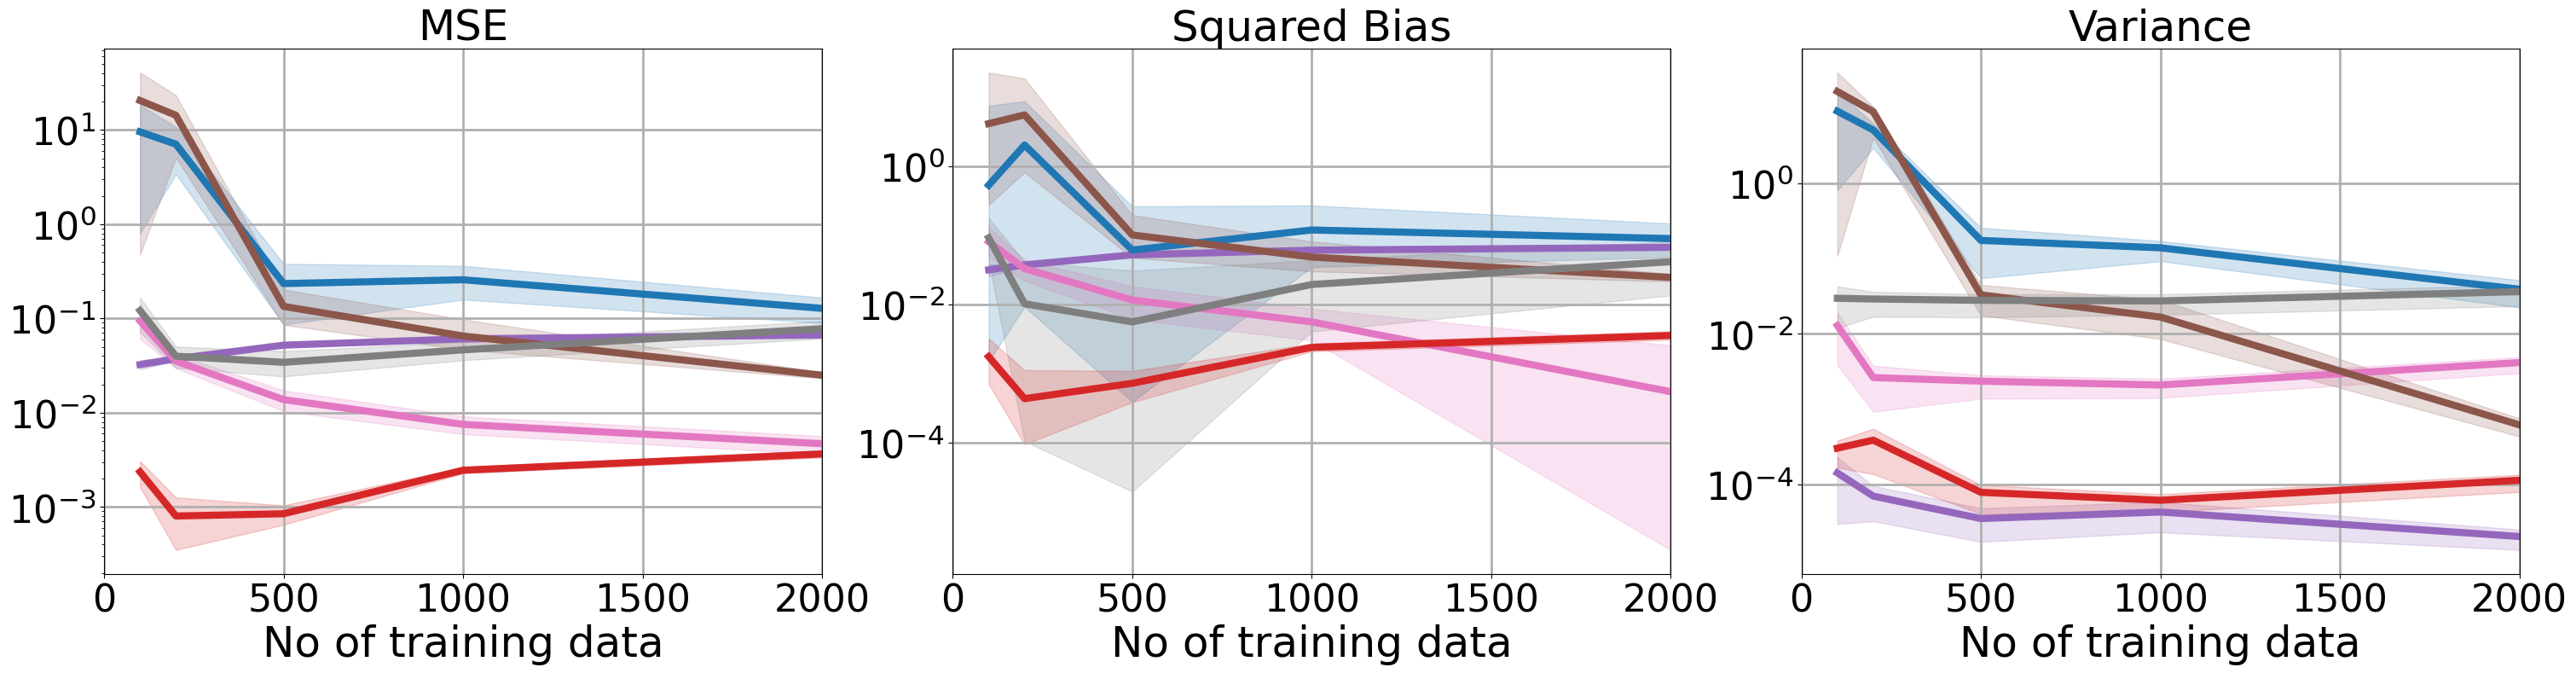
\includegraphics[width=1\textwidth]{figures/mr/multiclass/ope_vs_ntr_neval_1000_pendigits_alpha_0_6.png}
	    \subcaption{Results with varying $m$ for $\alpha^\ast=0.6$ and $n = 1000$}
	    \label{subfig:pen-tr}
	\end{subfigure}
    \caption{Results for PenDigits dataset}
    \label{fig:pendigits}
\end{figure}

\begin{figure}[h!]
    \centering
	\begin{subfigure}{0.8\textwidth}
	    \centering
	    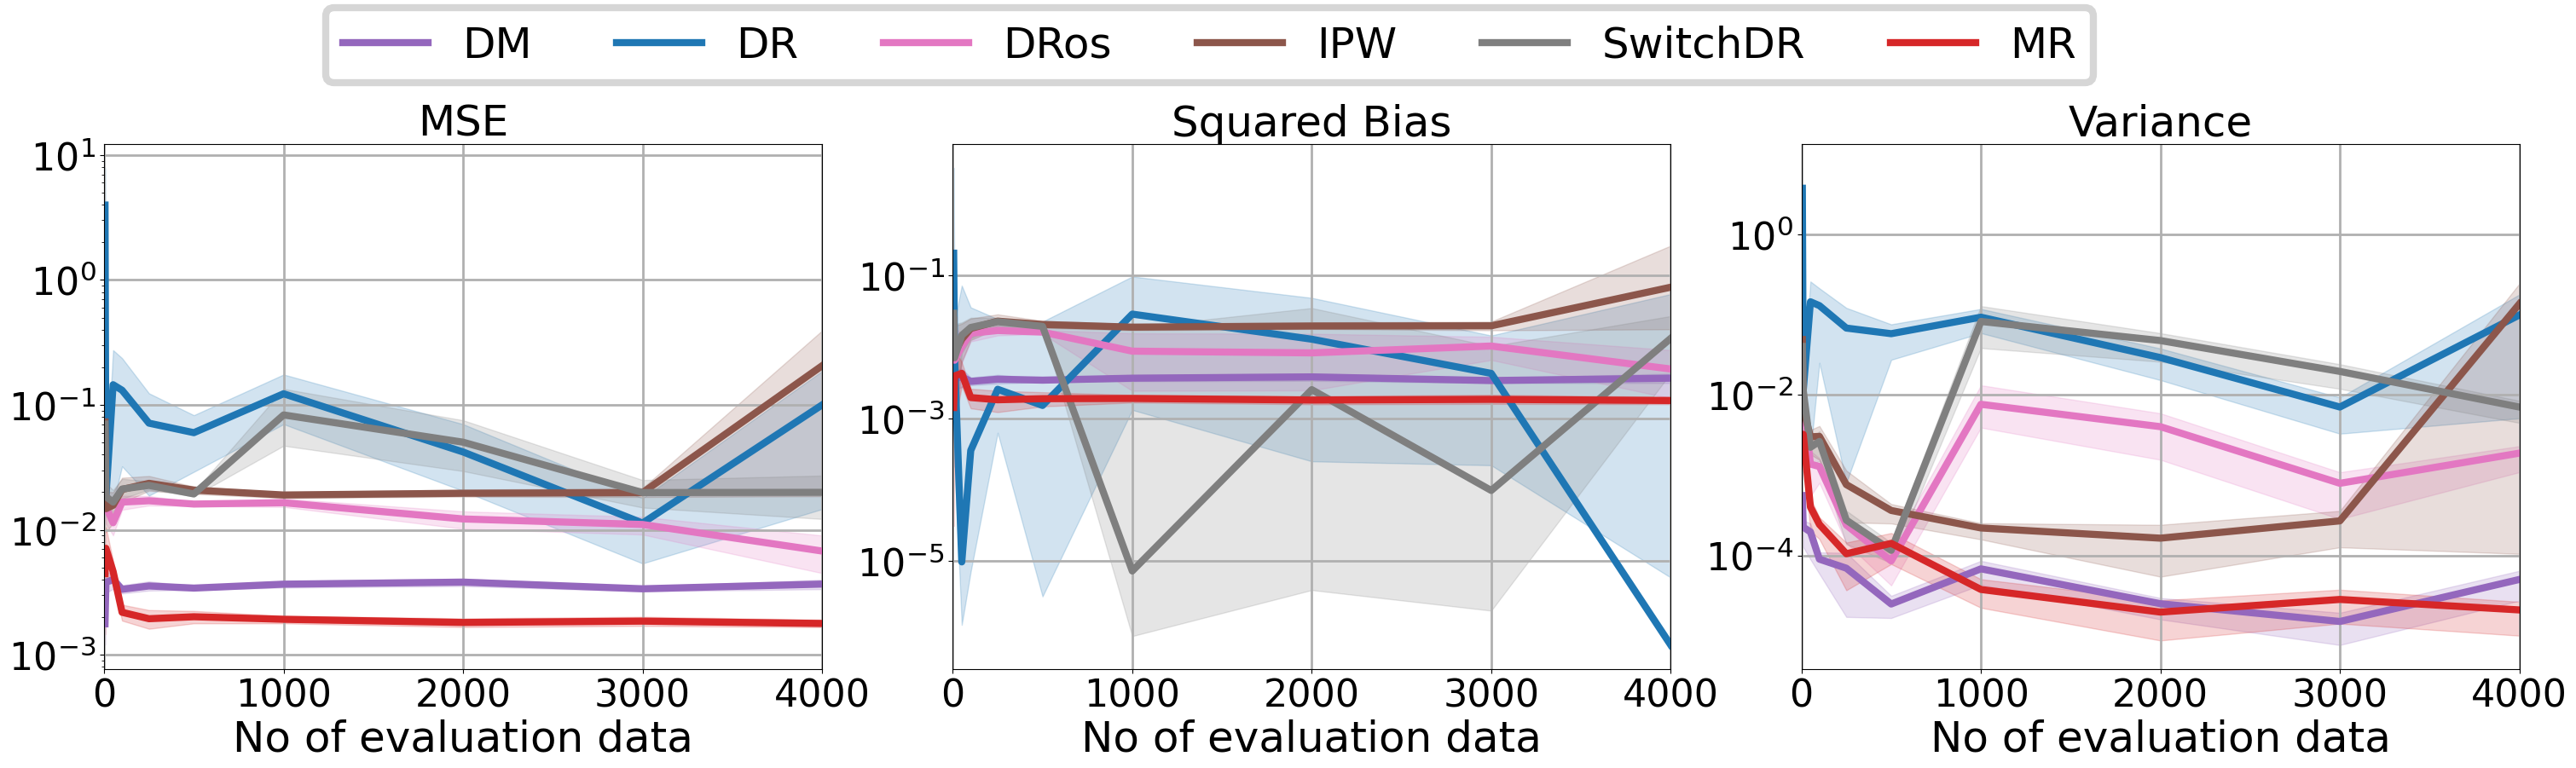
\includegraphics[width=1\textwidth]{figures/mr/multiclass/ope_vs_n_alphatar_0_2_satimage_ntr1000.png}
	    \subcaption{Results with varying $n$ for $\alpha^\ast = 0.2$ and $m=1000$}
	    \label{subfig:sat-neval}
	\end{subfigure}\\
	\begin{subfigure}{0.8\textwidth} 
	    \centering
	    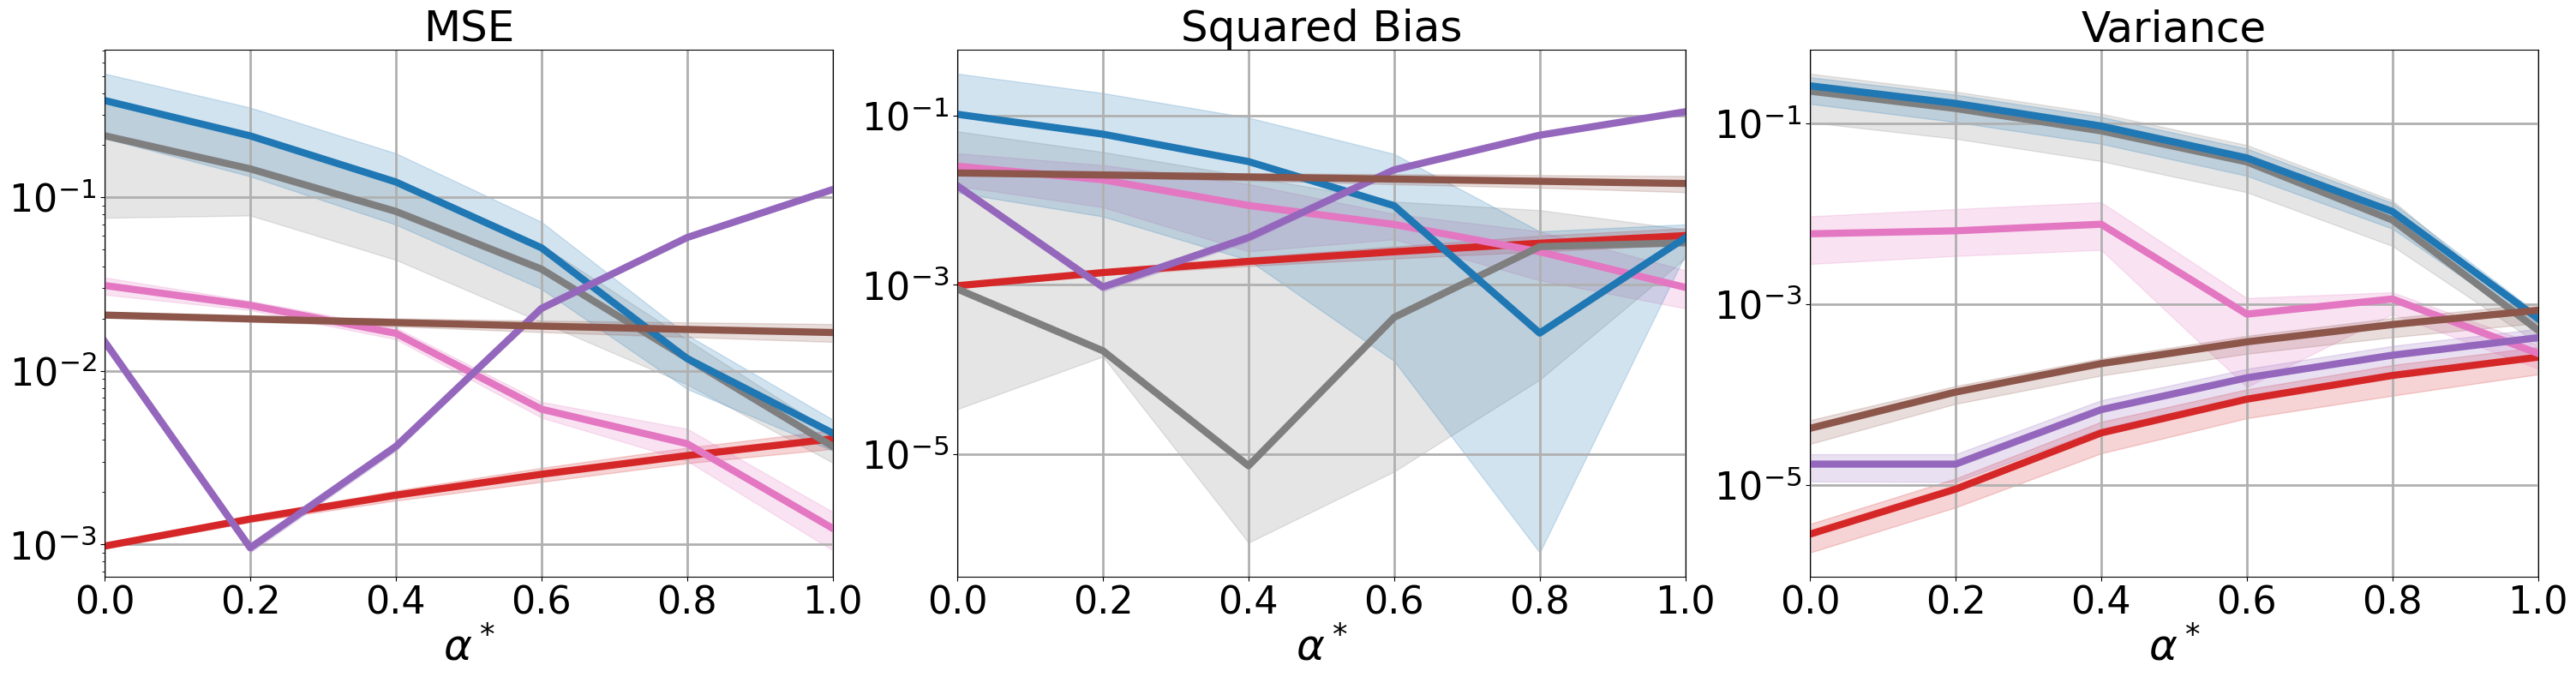
\includegraphics[width=1\textwidth]{figures/mr/multiclass/ope_vs_alphatar_neval_1000_satimage_ntr_1000.png}
	    \subcaption{Results with varying $\alpha^\ast$ for $n = 1000$}
	    \label{subfig:sat-ae}
	\end{subfigure}\\
 	\begin{subfigure}{0.8\textwidth} 
	    \centering
	    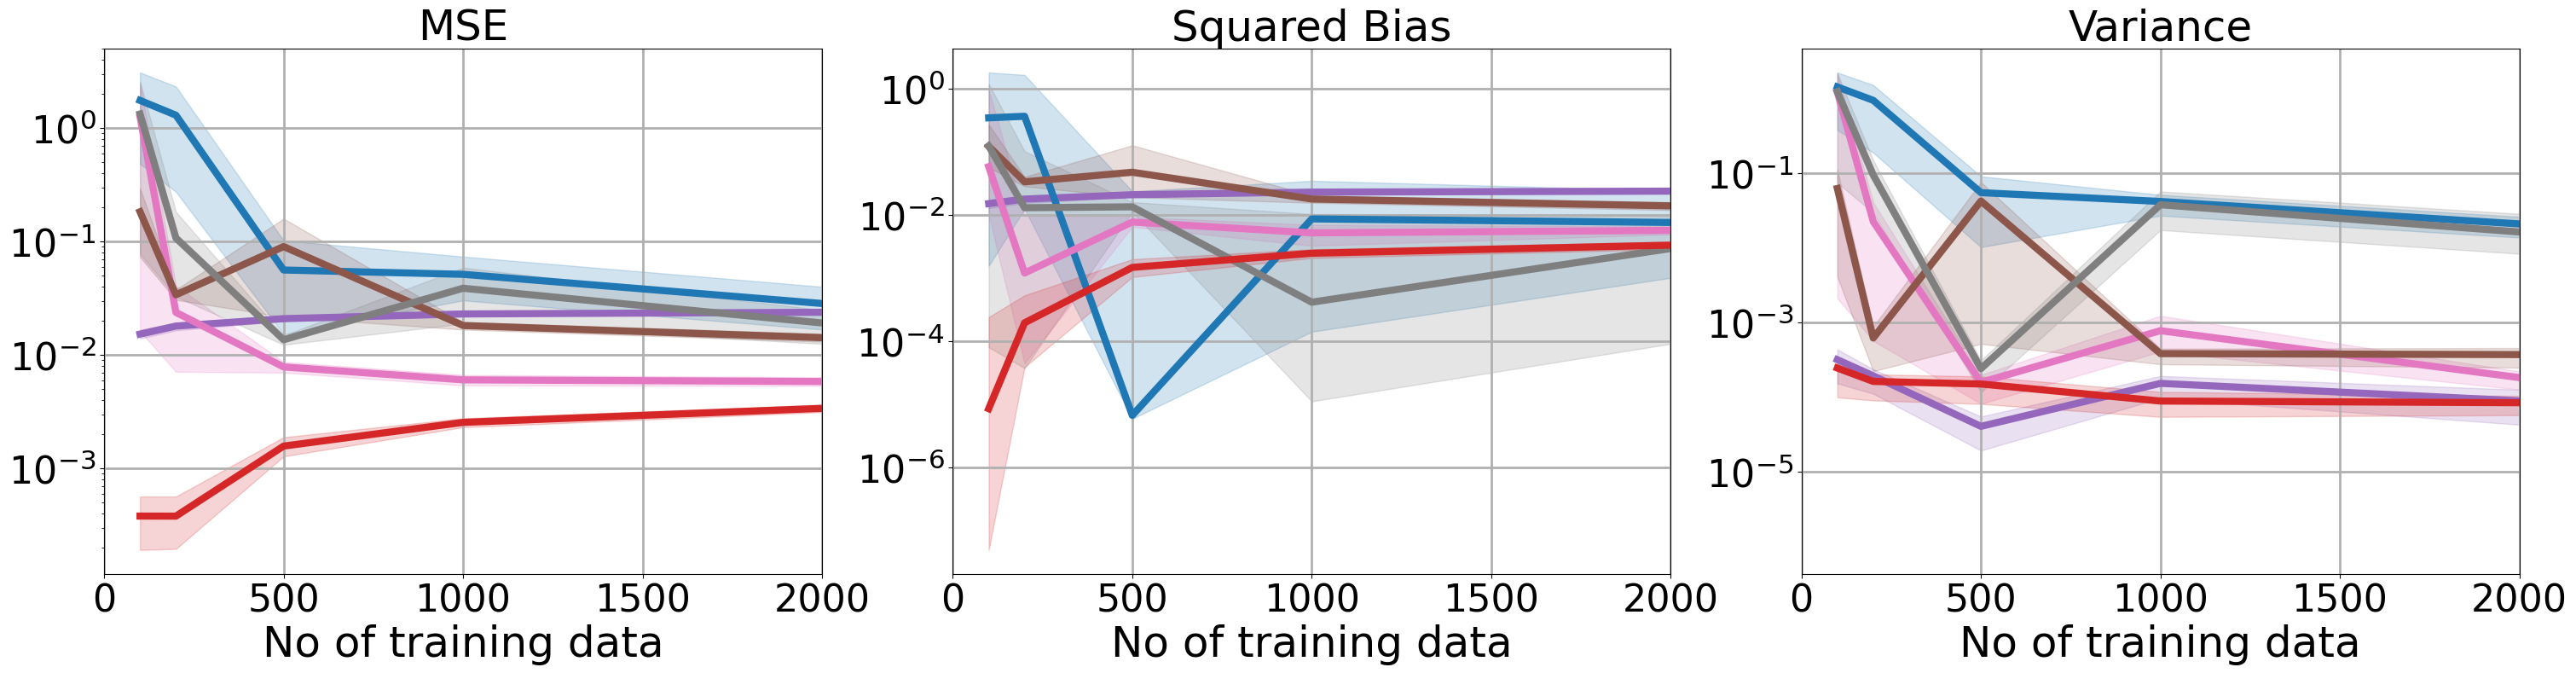
\includegraphics[width=1\textwidth]{figures/mr/multiclass/ope_vs_ntr_neval_1000_satimage_alpha_0_6.png}
	    \subcaption{Results with varying $m$ for $\alpha^\ast=0.6$ and $n = 1000$}
	    \label{subfig:sat-tr}
	\end{subfigure}
    \caption{Results for SatImage dataset}
    \label{fig:satimage}
\end{figure}

\begin{figure}[h!]
    \centering
	\begin{subfigure}{0.8\textwidth}
	    \centering
	    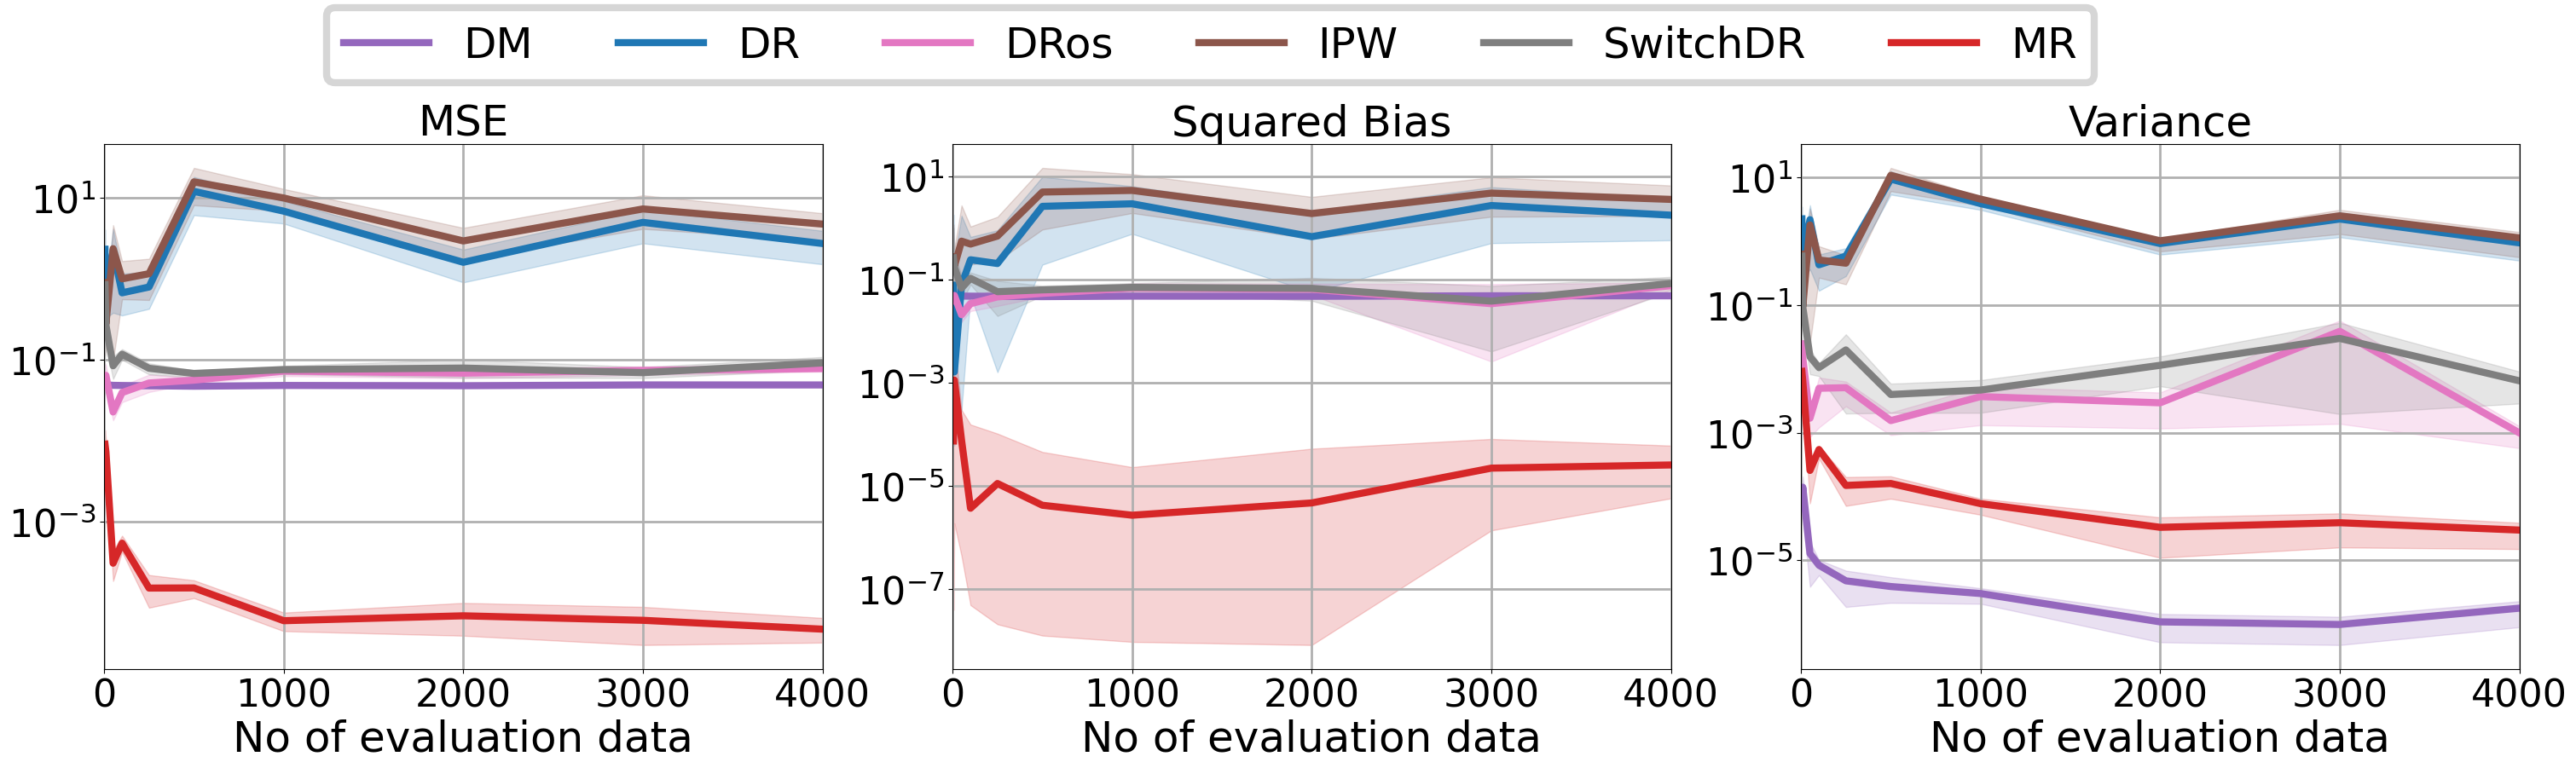
\includegraphics[width=1\textwidth]{figures/mr/multiclass/ope_vs_n_alphatar_0_2_letter_ntr1000.png}
	    \subcaption{Results with varying $n$ for $\alpha^\ast = 0.2$ and $m=1000$}
	    \label{subfig:letter-neval}
	\end{subfigure}\\
	\begin{subfigure}{0.8\textwidth} 
	    \centering
	    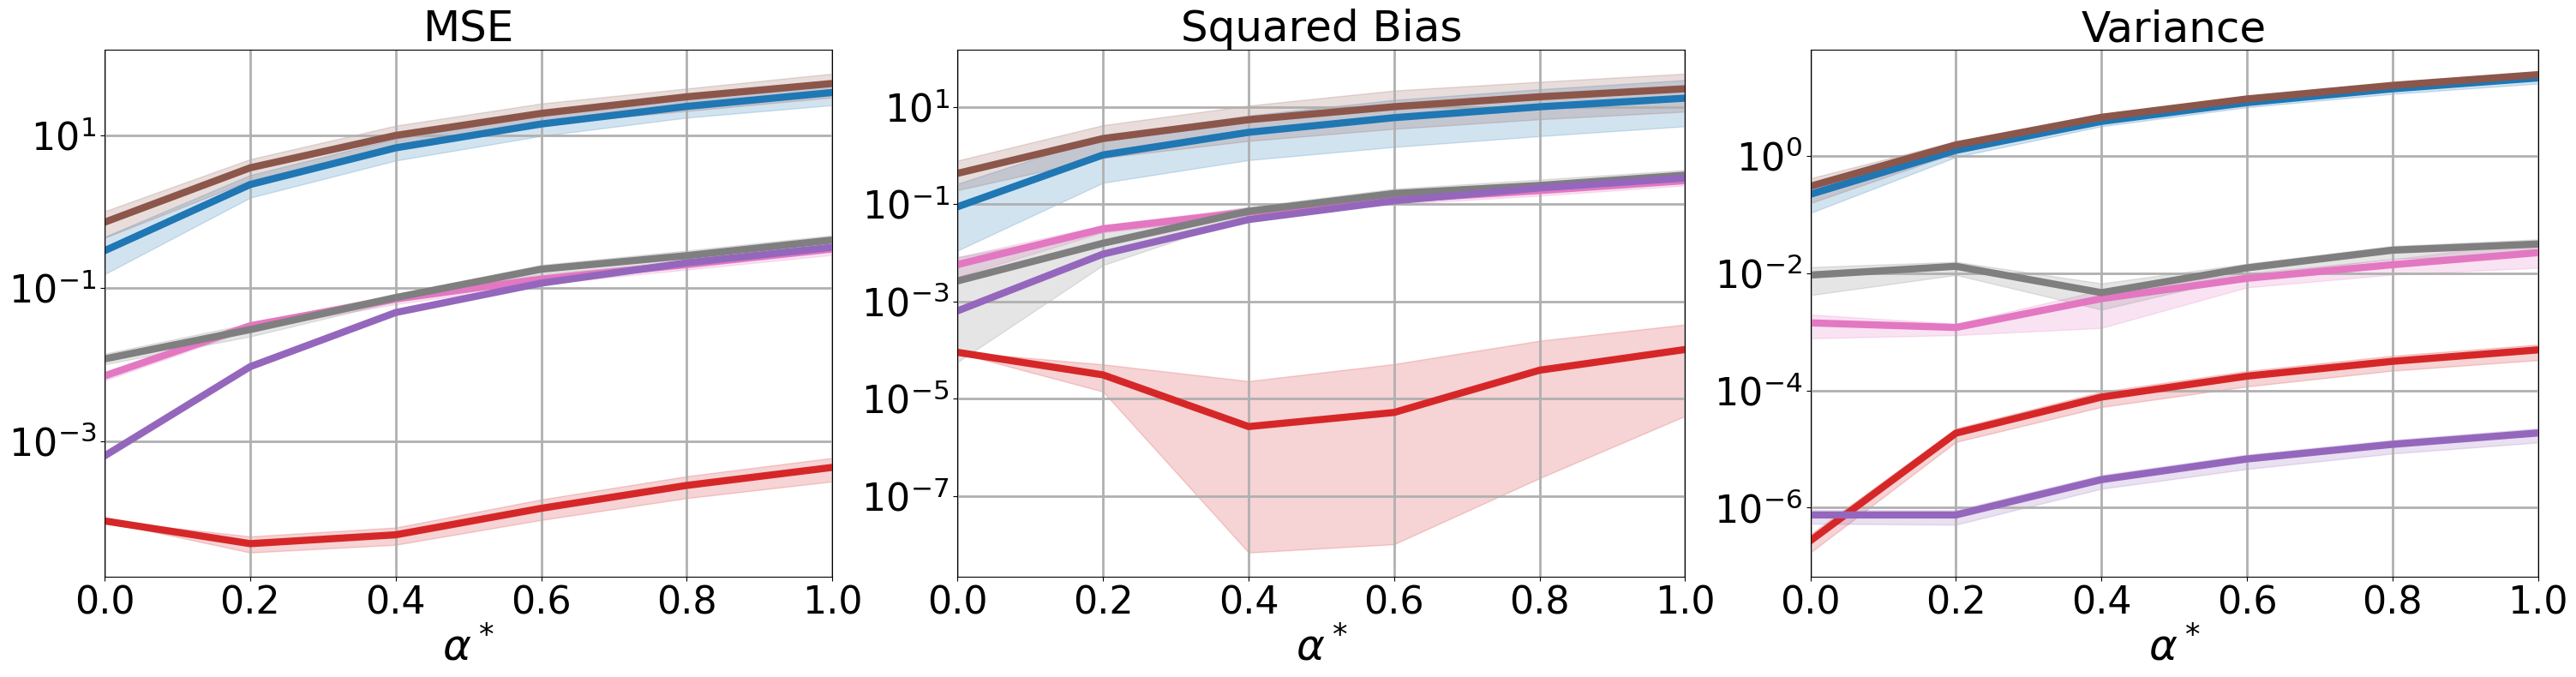
\includegraphics[width=1\textwidth]{figures/mr/multiclass/ope_vs_alphatar_neval_1000_letter_ntr_1000.png}
	    \subcaption{Results with varying $\alpha^\ast$ for $m = n = 1000$}
	    \label{subfig:letter-ae}
	\end{subfigure}\\
        \begin{subfigure}{0.8\textwidth} 
	    \centering
	    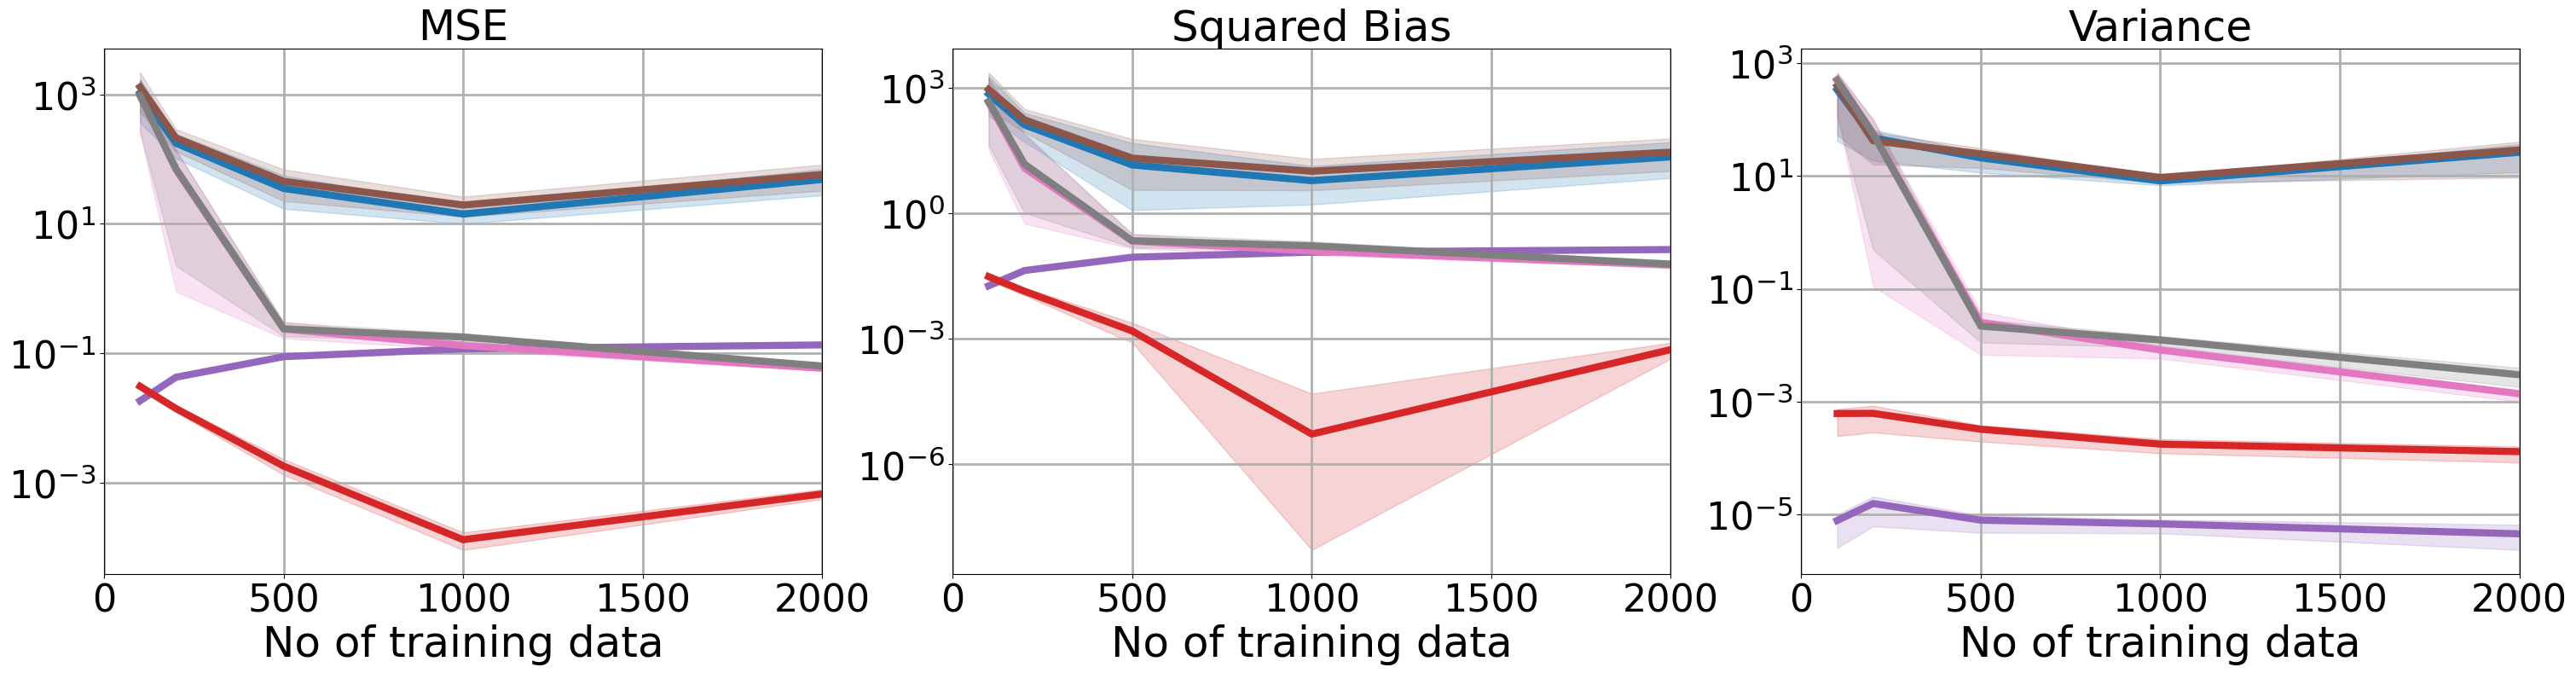
\includegraphics[width=1\textwidth]{figures/mr/multiclass/ope_vs_ntr_neval_1000_letter_alpha_0_6.png}
	    \subcaption{Results with varying $m$ for $\alpha^\ast=0.6$ and $n = 1000$}
	    \label{subfig:letter-tr}
	\end{subfigure}
    \caption{Results for Letter dataset}
    \label{fig:letter}
\end{figure}

\begin{figure}[h!]
    \centering
	\begin{subfigure}{0.8\textwidth}
	    \centering
	    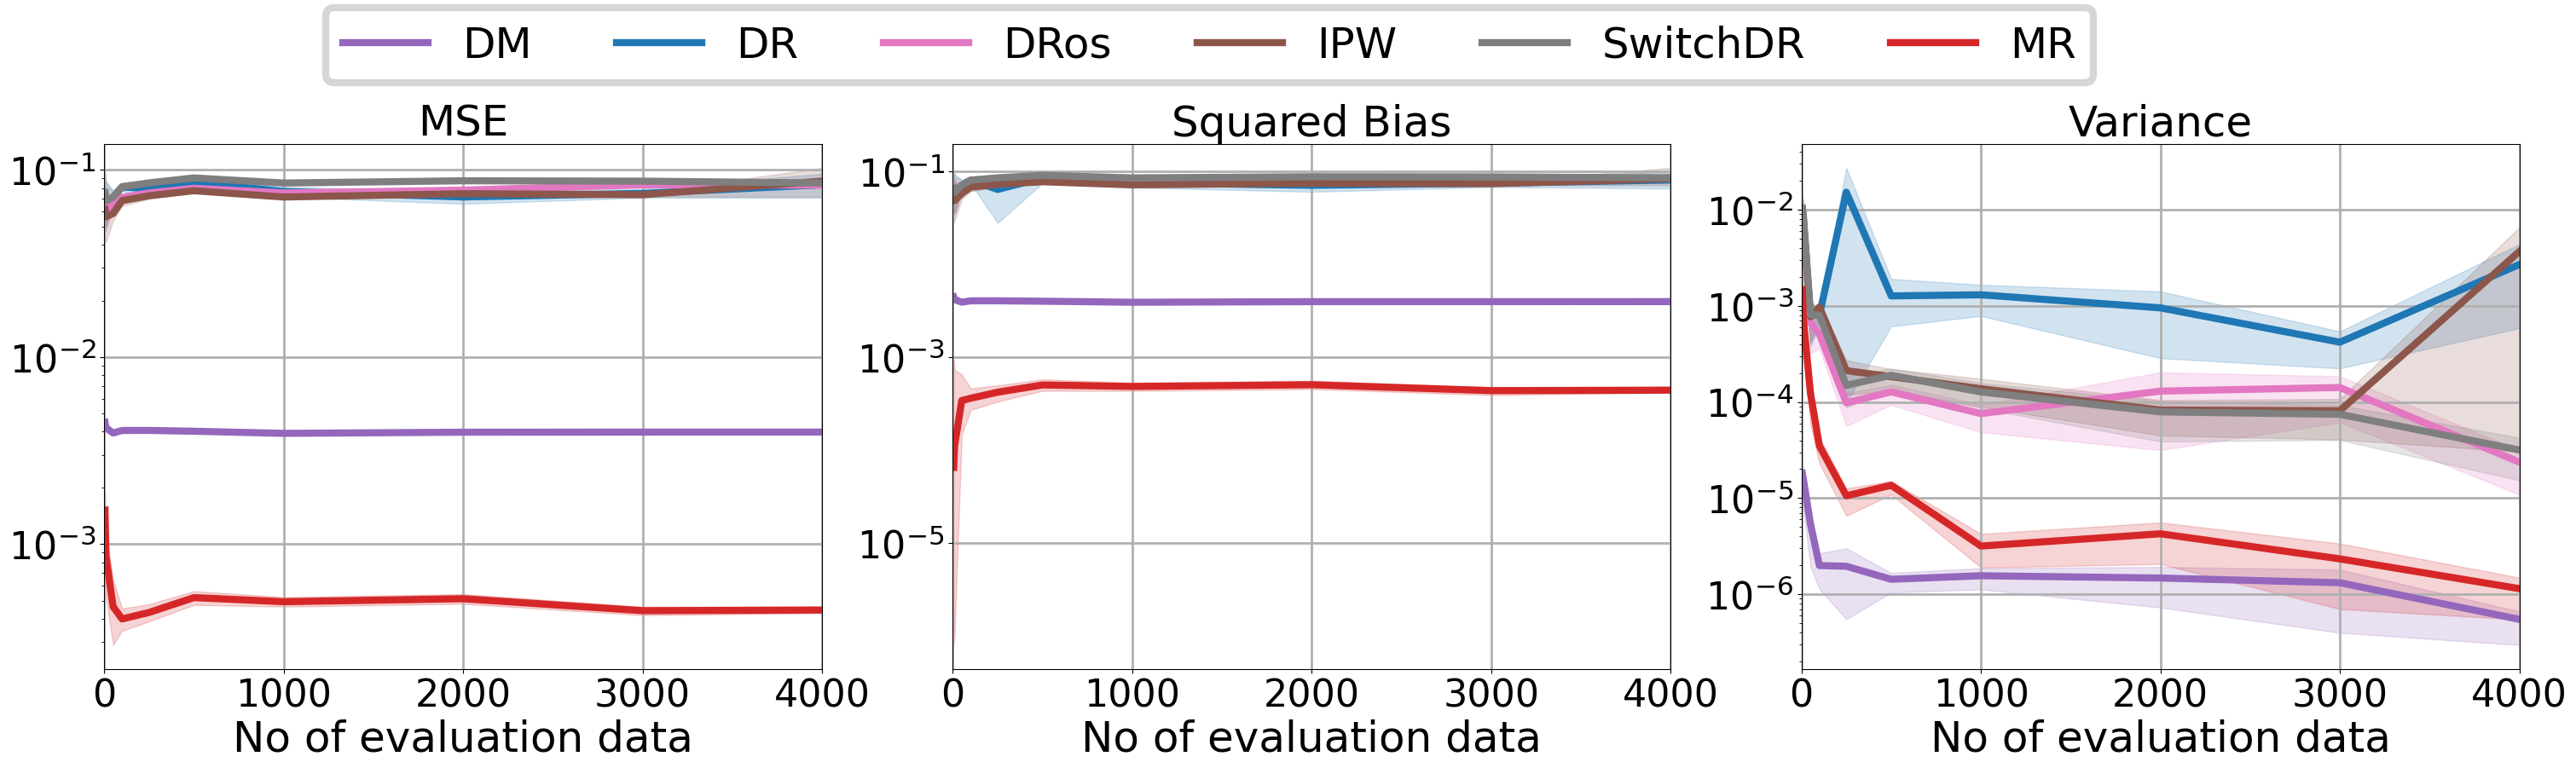
\includegraphics[width=1\textwidth]{figures/mr/multiclass/ope_vs_n_alphatar_0_2_mnist_ntr1000.png}
	    \subcaption{Results with varying $n$ for $\alpha^\ast = 0.2$ and $m=1000$}
	    \label{subfig:mnist-neval}
	\end{subfigure}\\
	\begin{subfigure}{0.8\textwidth} 
	    \centering
	    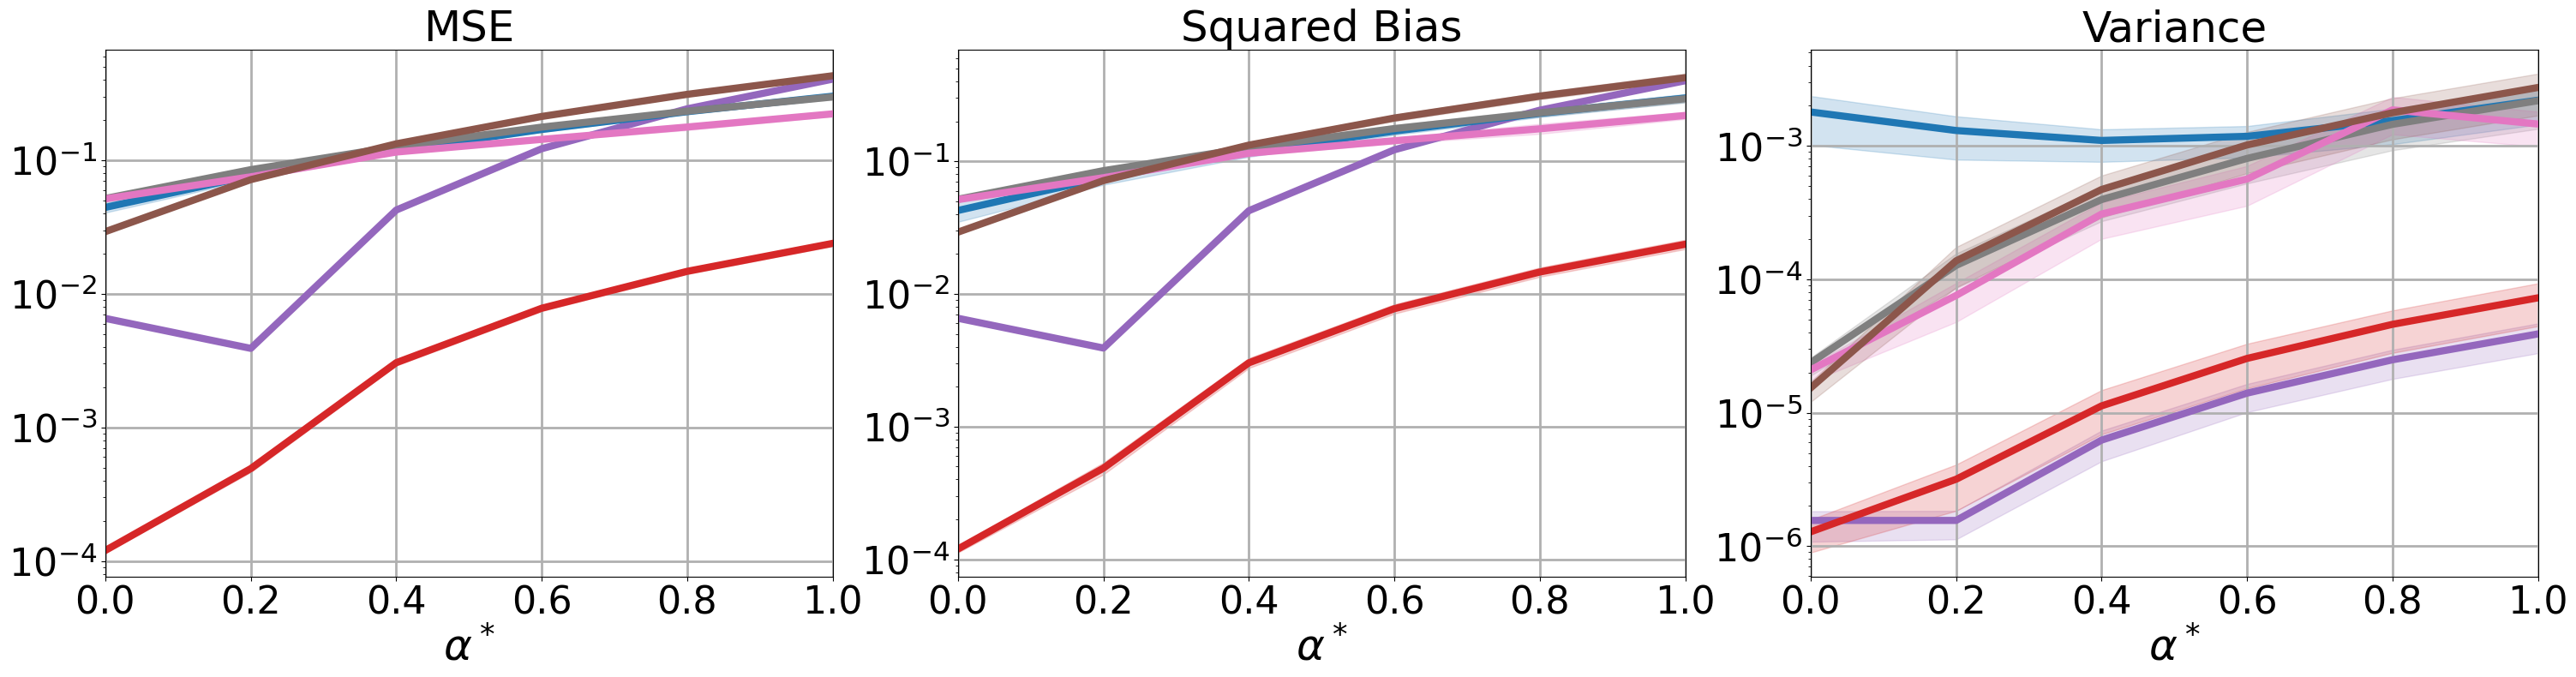
\includegraphics[width=1\textwidth]{figures/mr/multiclass/ope_vs_alphatar_neval_1000_mnist_ntr_1000.png}
	    \subcaption{Results with varying $\alpha^\ast$ for $m= n = 1000$}
	    \label{subfig:mnist-ae}
	\end{subfigure}\\
 	\begin{subfigure}{0.8\textwidth} 
	    \centering
	    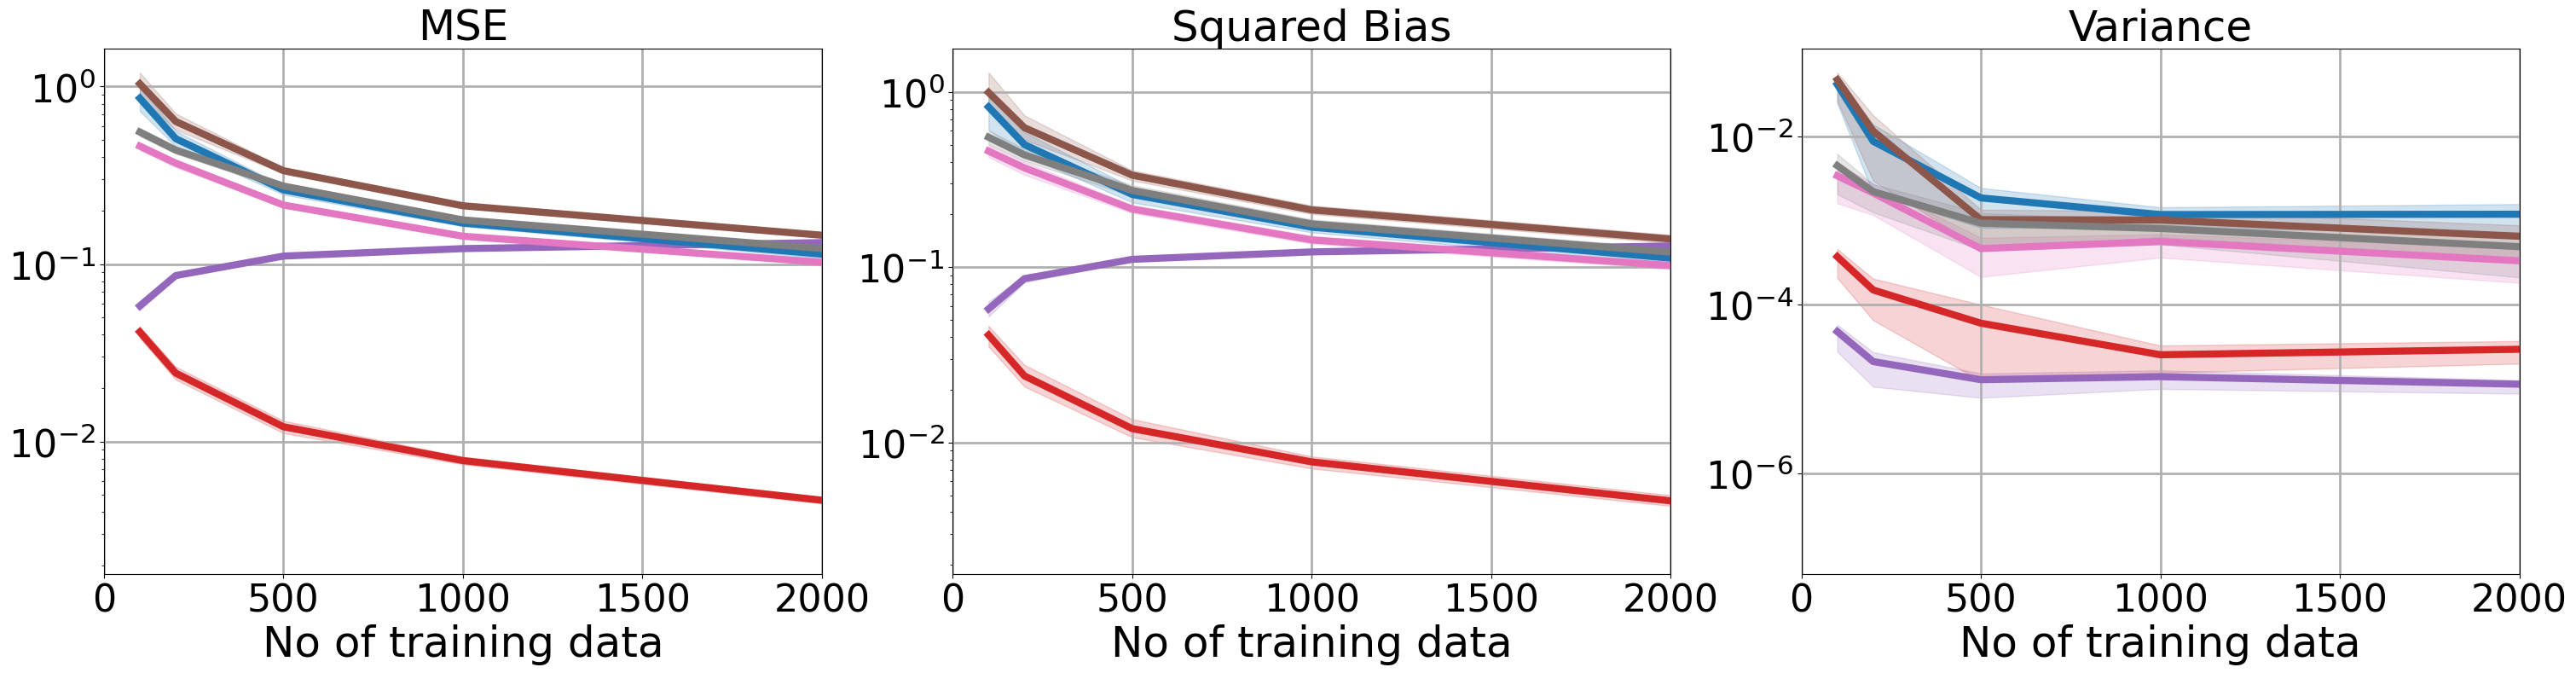
\includegraphics[width=1\textwidth]{figures/mr/multiclass/ope_vs_ntr_neval_1000_mnist_alpha_0_6.png}
	    \subcaption{Results with varying $m$ for $\alpha^\ast=0.6$ and $n = 1000$}
	    \label{subfig:mnist-tr}
	\end{subfigure}
    \caption{Results for Mnist dataset}
    \label{fig:mnist}
\end{figure}

\begin{figure}[h!]
    \centering
	\begin{subfigure}{0.8\textwidth}
	    \centering
	    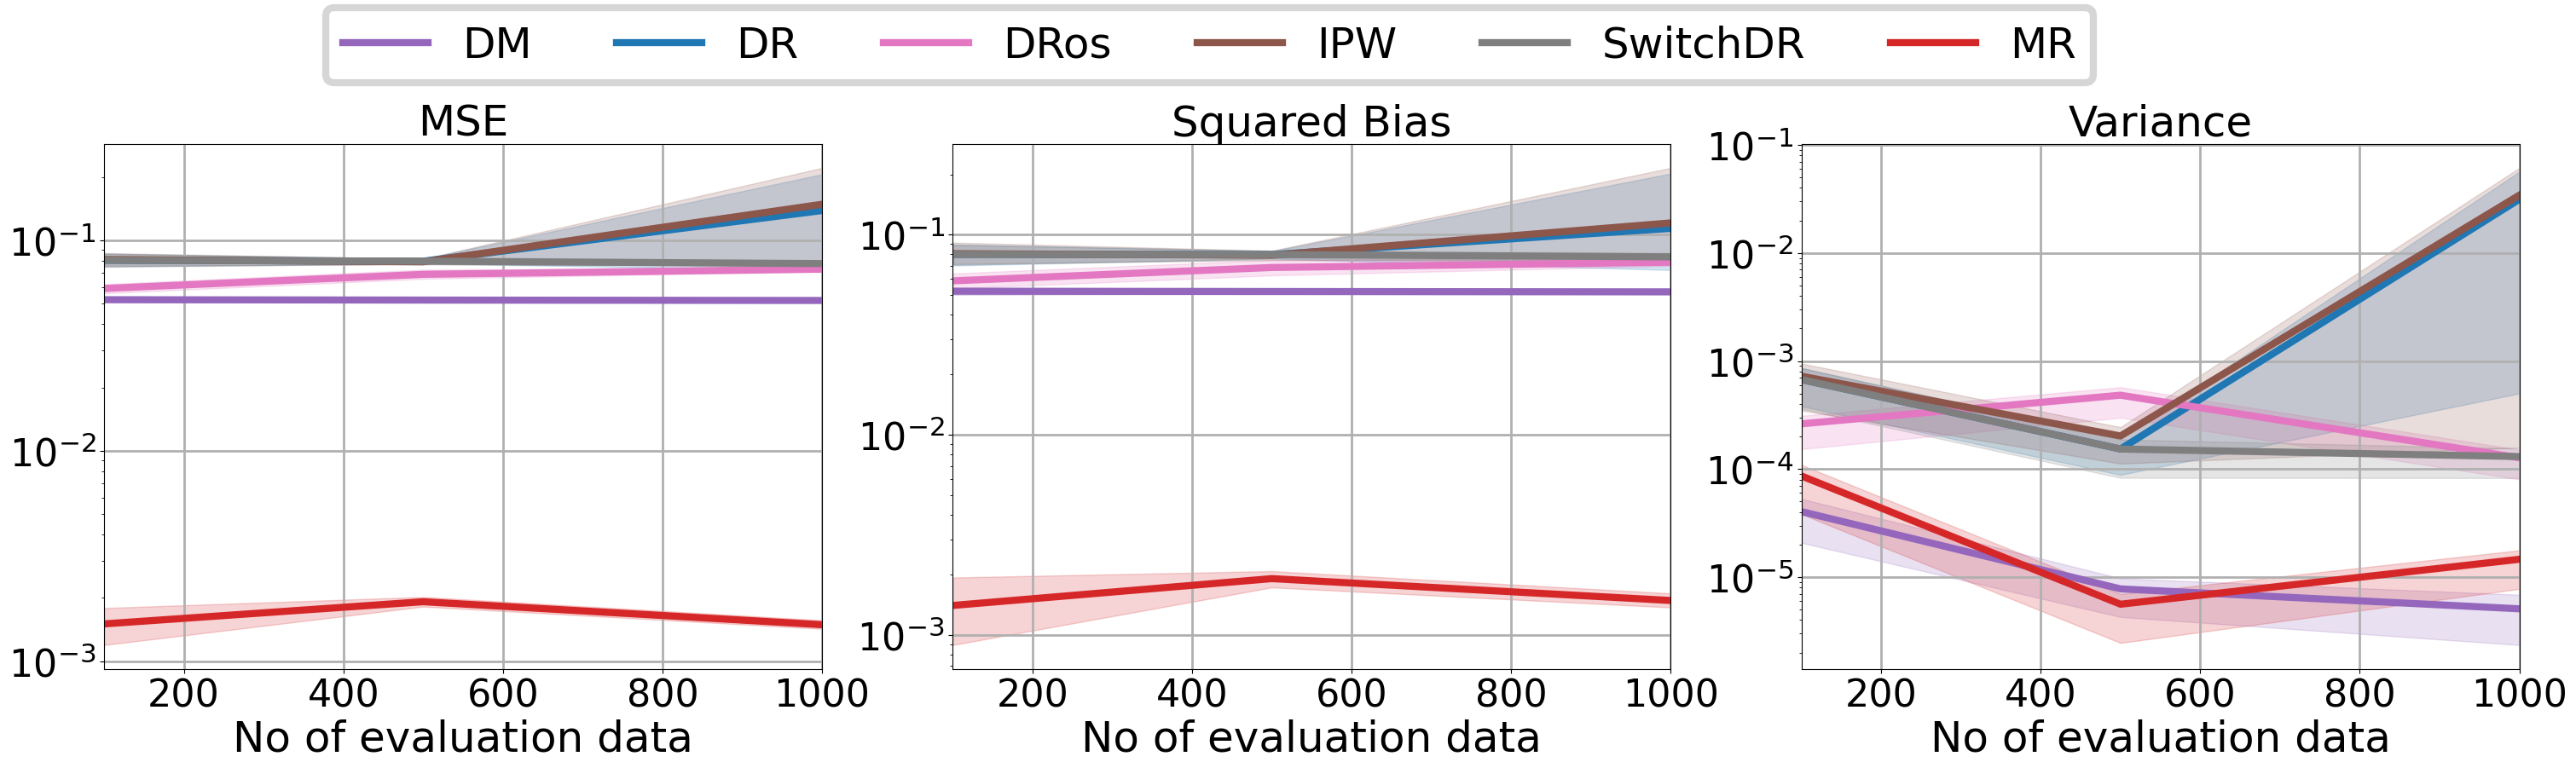
\includegraphics[width=1\textwidth]{figures/mr/multiclass/ope_vs_n_alphatar_0_2_digits_ntr500.png}
	    \subcaption{Results with varying $n$ for $\alpha^\ast = 0.2$ and $m=500$}
	    \label{subfig:digits-neval}
	\end{subfigure}\\
	\begin{subfigure}{0.8\textwidth} 
	    \centering
	    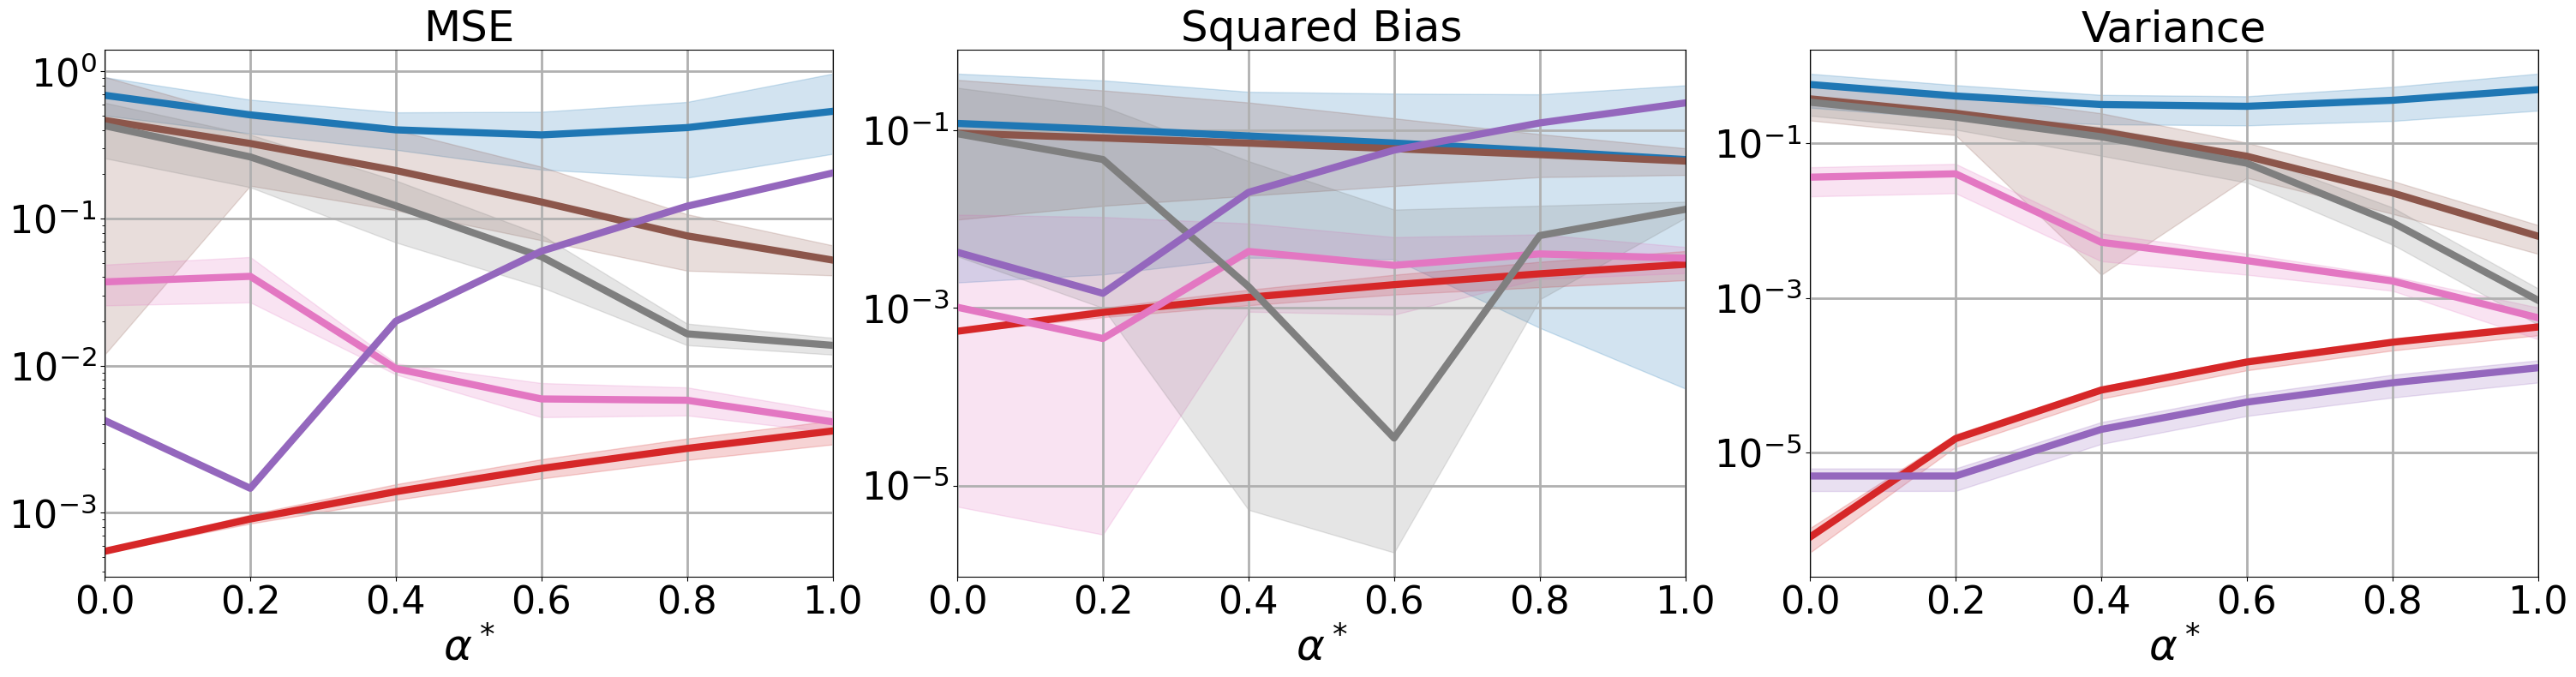
\includegraphics[width=1\textwidth]{figures/mr/multiclass/ope_vs_alphatar_neval_500_digits_ntr_1000.png}
	    \subcaption{Results with varying $\alpha^\ast$ for $n = 500$ and $m=1000$}
	    \label{subfig:digits-ae}
	\end{subfigure}\\
 	\begin{subfigure}{0.8\textwidth} 
	    \centering
	    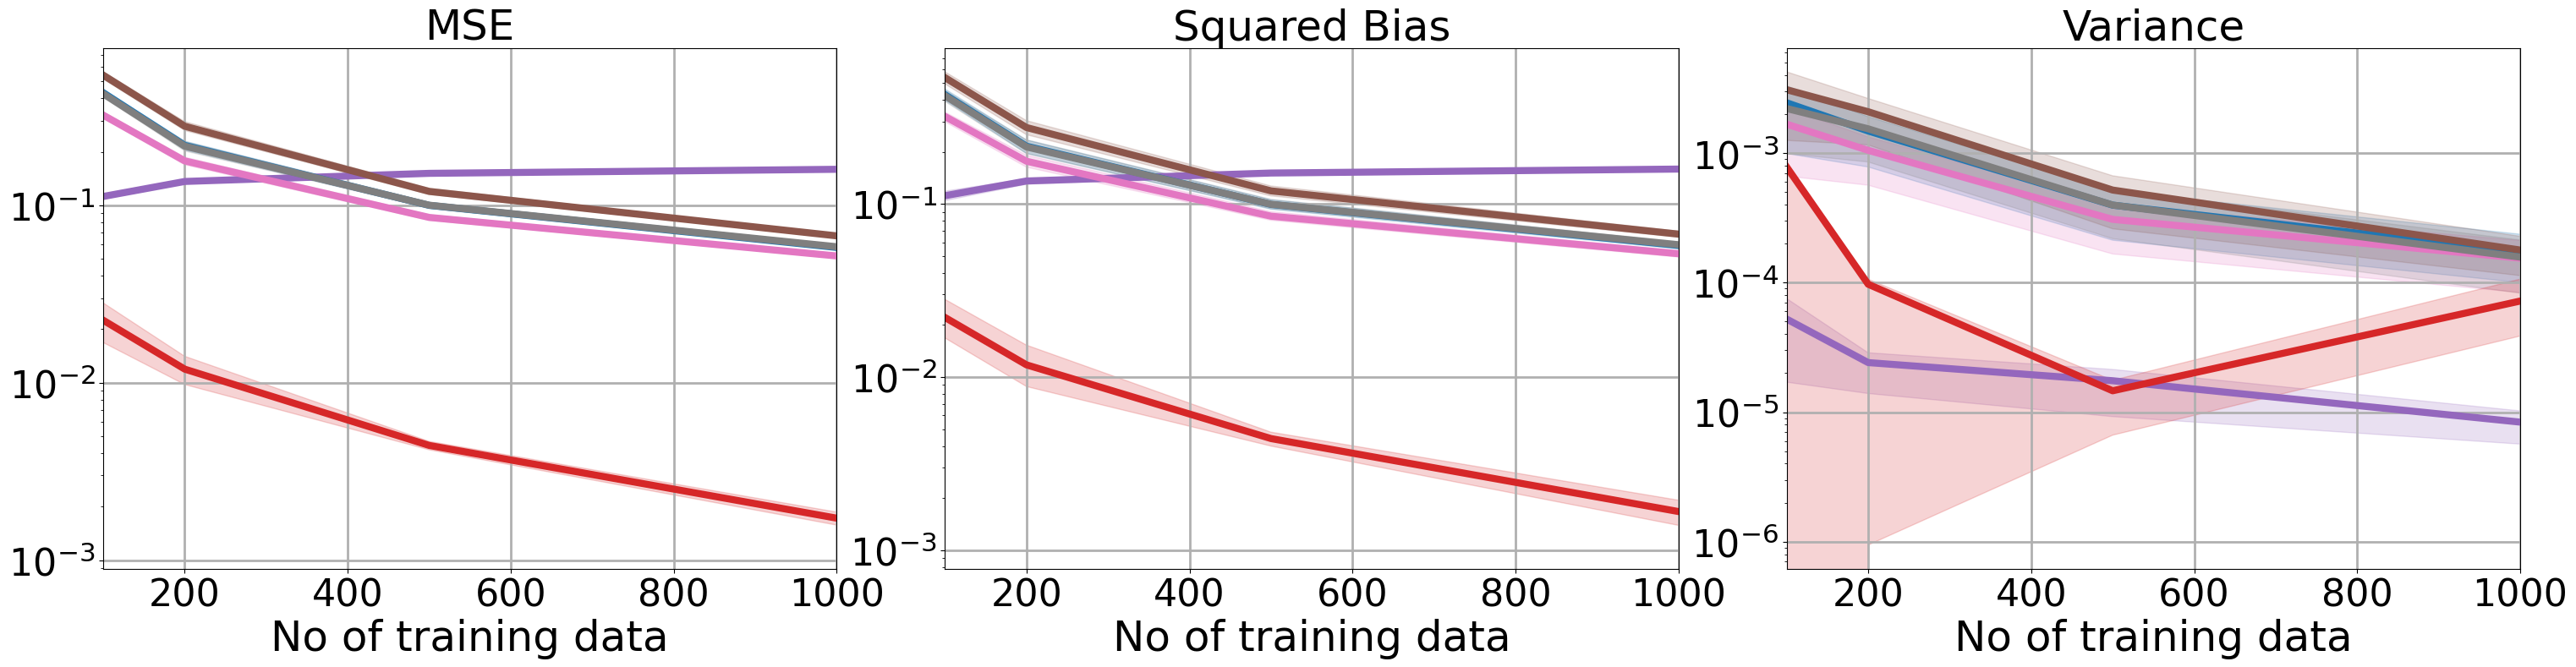
\includegraphics[width=1\textwidth]{figures/mr/multiclass/ope_vs_ntr_neval_500_digits_alpha_0_6.png}
	    \subcaption{Results with varying $m$ for $\alpha^\ast=0.6$ and $n = 500$}
	    \label{subfig:digits-tr}
	\end{subfigure}
    \caption{Results for Digits dataset. Note that compared to other datasets we consider smaller maximum dataset sizes $m,n$ here as the total number of available datapoints was 1797.}
    \label{fig:digits}
\end{figure}

\begin{figure}[h!]
    \centering
	\begin{subfigure}{0.8\textwidth}
	    \centering
	    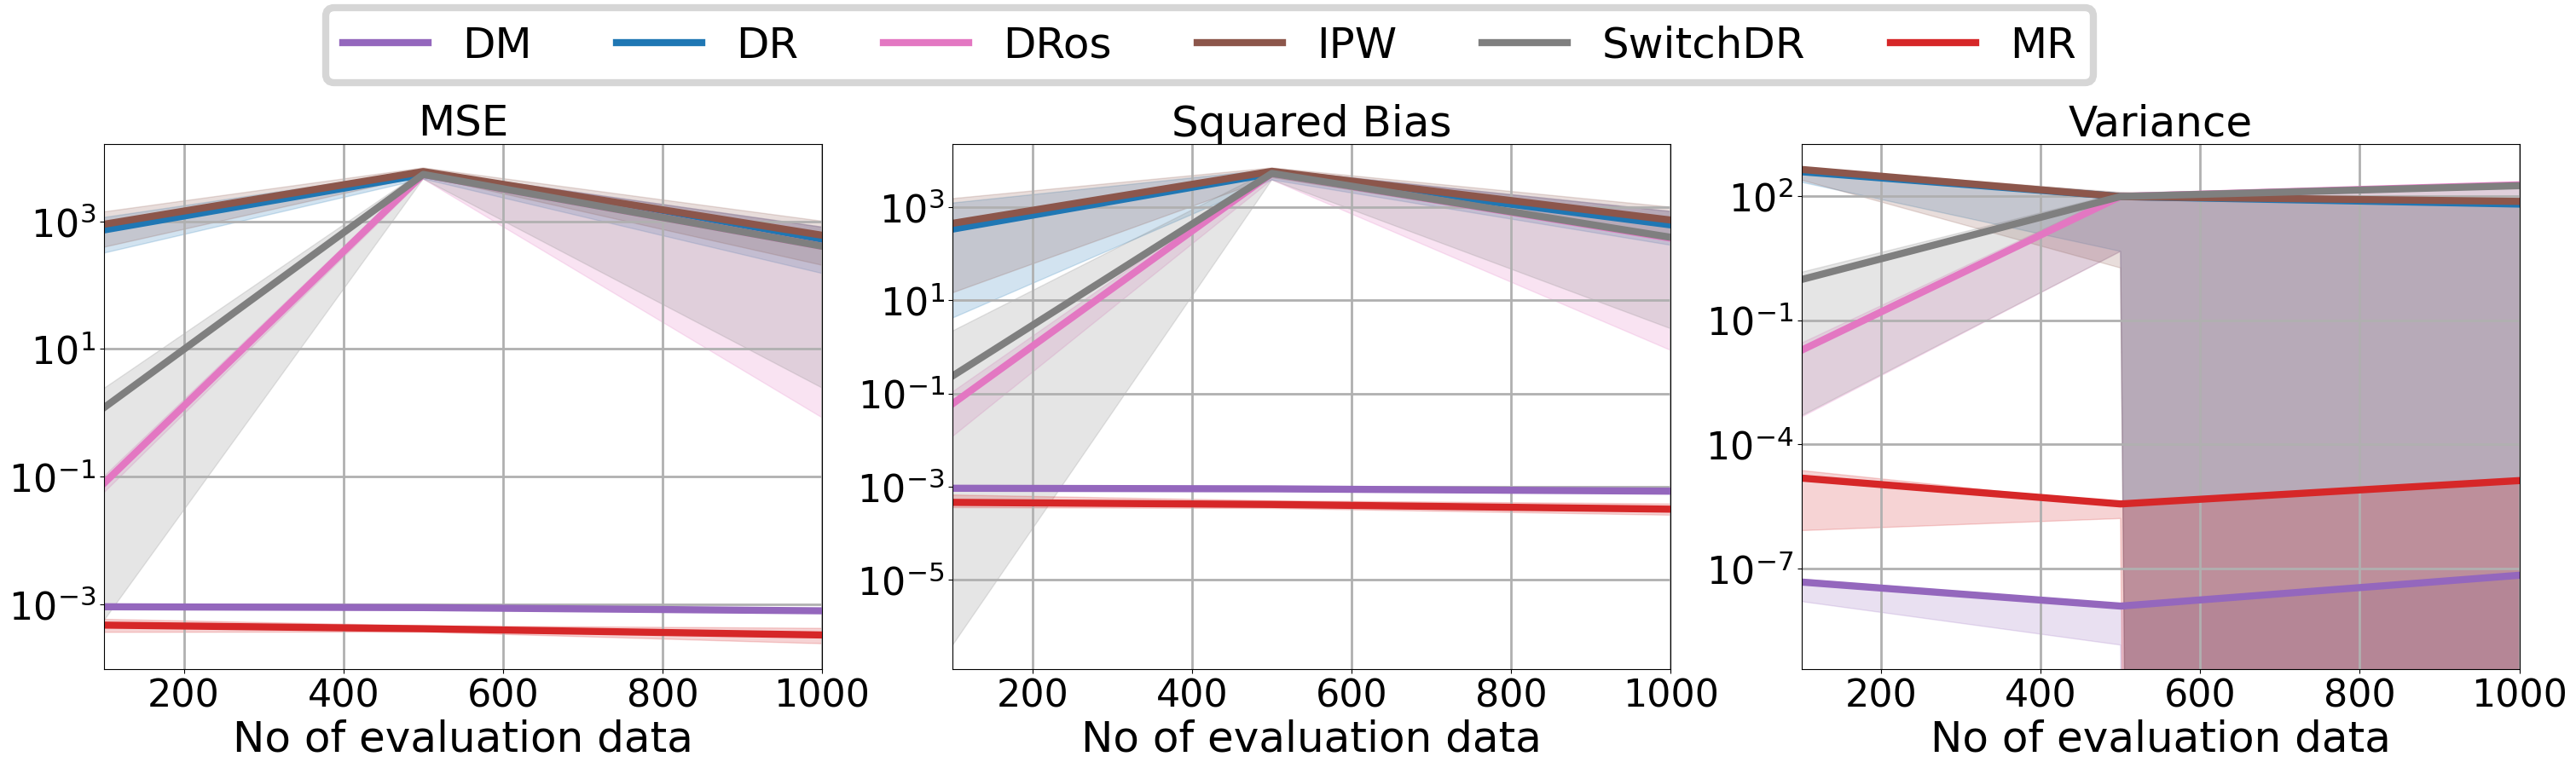
\includegraphics[width=1\textwidth]{figures/mr/multiclass/cifar100n_eval.png}
	    \subcaption{Results with varying $n$ for $\alpha^\ast = 0.4$ and $m=2000$}
	    \label{subfig:cifar100-neval}
	\end{subfigure}\\
	\begin{subfigure}{0.8\textwidth} 
	    \centering
	    \includegraphics[width=1\textwidth]{figures/mr/multiclass/cifar100alpha_star.png}
	    \subcaption{Results with varying $\alpha^\ast$ for $n = 100$ and $m=2000$}
	    \label{subfig:cifar-ae}
	\end{subfigure}\\
 	\begin{subfigure}{0.8\textwidth} 
	    \centering
	    \includegraphics[width=1\textwidth]{figures/mr/multiclass/cifar100n_train.png}
	    \subcaption{Results with varying $m$ for $\alpha^\ast=0.4$ and $n = 100$}
	    \label{subfig:cifar100-tr}
	\end{subfigure}
    \caption{Results for CIFAR-100 dataset.}
    \label{fig:cifar100}
\end{figure}

\subsection{Application to Average Treatment Effect (ATE) estimation}\label{app:ate-empirical}
In this subsection, we provide additional details for our experiment applying MR to the problem of ATE estimation presented in the main text. We begin by describing the dataset being used in this experiment.

\paragraph{Twins dataset}
We use the Twins dataset as studied by \cite{louizos2017causal}, which comprises data from twin births in the USA between 1989-1991. The treatment $a=1$ corresponds to being born the heavier twin and the outcome $Y$ corresponds to the mortality of each of the twins in their first year of life. Since the data includes records for both twins, their outcomes would be considered as the two potential outcomes. Specifically, $Y(1)$ corresponds to the mortality of the heavier twin (and likewise for $Y(0)$). Closely following the methodology of \cite{louizos2017causal}, we only chose twins which are the same sex and weigh less than 2kgs. This provides us with a dataset of 11984 pairs of twins. 

The mortality rate for the lighter twin is 18.9\% and for the heavier twin is 16.4\%, leading to the ATE value being $\theta_\ate = -2.5\%$. For each twin-pair we obtained 46 covariates relating to the parents, the pregnancy and birth. 

\paragraph{Treatment assignment}
To simulate an observational study, we selectively hide one of the two twins by defining the treatment variable $A$ which depends on the feature \emph{GESTAT10}. This feature, which takes integer values from 0 to 9, is obtained by grouping the number of gestation weeks prior to birth into 10 groups.
Then we sample actions $A$ as follows, 
\[
A \mid X \sim \textup{Bern}(Z/10),
\]
where $Z$ is \emph{GESTAT10}, and $X$ are all the 46 features corresponding to a twin pair (including \emph{GESTAT10}). 

Using the treatment assignments defined above, we generate the observational data by selectively hiding one of the two twins from each pair. Next, we randomly split this dataset into training and evaluation datasets of sizes $m$ and $n$ respectively. In this experiment, we consider $m=5000$ training datapoints. 

\paragraph{Baselines}
Recall that ATE estimation can be formulated as the difference between off-policy values of deterministic policies $\pi^{(1)} \coloneqq \ind(A=1)$ and $\pi^{(0)} \coloneqq \ind(A=0)$. Therefore, any OPE estimator can be applied to ATE estimation. In this experiment, we compare our estimator against the baselines considered in our OPE experiments in Section \ref{subsec:additional-experiments-classification}. This includes the Direct Method (DM), IPW and DR estimators as well as Switch-DR \citep{wang2017optimal} and DR with Optimistic Shrinkage (DRos) \citep{su2020doubly}. To estimate $\hat{q}(x, a)$ for DM and DR estimators, we use multi-layer perceptrons (MLP) trained on the $m$ training datapoints. Additionally, we estimate the behaviour policy $\hatbeh$ using random forest classifier trained on the full training dataset. 

Since the outcome in this experiment is binary, we estimate the weights $w(y) = \Ebeh[\hat{\rho}(A, X)\mid Y=y]$ directly by estimating the sample mean of $\hat{\rho}(A, X)$ for datapoints with $Y=y$. This means that the alternative method of estimating MR yields the same value as the default method. We therefore do not consider these estimators separately. Additionally, since there is no natural embedding $R$ of the covariate-action space which satisfies the conditional dependence Assumption \ref{assum:indep-general}, we do not consider the G-MIPS (or MIPS) estimator either.   
% We compare our estimator with Direct Method (DM), IPW and DR estimators for ATE. 
% In addition, we also consider Switch-DR \citep{wang2017optimal} and DR with Optimistic Shrinkage (DRos) \citep{su2020doubly}.


\paragraph{Performance metric}
For our evaluation, we consider the absolute error in ATE estimation, $\epsilon_\ate$, defined as:
\[
\epsilon_\ate \coloneqq | \hat{\theta}^{(n)}_\ate - \theta_\ate |.
\]
Here, $\hat{\theta}^{(n)}_\ate$ denotes the value of the ATE estimated using $n$ evaluation datapoints. For example, for the IPW estimator, the $\hat{\theta}^{(n)}_\ate$ can be written as:
\[
\hat{\theta}^{(n)}_\ate = \ateipw = \frac{1}{n} \sum_{i=1}^n \left(\frac{\ind(a_i=1)-\ind(a_i=0)}{\hatbeh(a_i\mid x_i)}\right)\, y_i.
\]

All results for this experiment are provided in the main text.

\subsection{Additional synthetic data experiments} \label{sec:app-additional-results}
\begin{figure}[ht]
     \centering
     \begin{subfigure}[b]{0.8\textwidth}
         \centering
         \includegraphics[width=\textwidth]{figures/mr/all_baselines/ope_vs_neval_nac_100_alphatar_0.4_dimc_1000_ntrain_100000.png}
         \caption{$d=1000$, $n_{a}=100$, $\alpha^\ast = 0.4$.}
         \label{fig:mse-vs-neval-conf2a}
     \end{subfigure}\\
     \begin{subfigure}[b]{0.8\textwidth}
         \centering
         \includegraphics[width=\textwidth]{figures/mr/all_baselines/ope_vs_neval_dimc_10000_alphatar_0.4_nac_100_ntrain_100000.png}
         \caption{$d=10000$, $n_{a}=100$, $\alpha^\ast = 0.4$.}
         \label{fig:mse-vs-neval-conf2b}
     \end{subfigure}
     \caption{Results with varying size of evaluation dataset $n$.}
     \label{fig:mse-vs-neval-conf2}
 \end{figure}

 \begin{figure}[ht]
     \centering
    \begin{subfigure}[b]{0.8\textwidth}
         \centering
         \includegraphics[width=\textwidth]{figures/mr/all_baselines/ope_vs_alphatar_dimc_1000_nac_100_neval_100_ntrain_10000.png}
         \caption{$d=1000$, $n_{a}=100$, $n = 100$.}
         \label{fig:mse-vs-betatar-conf2a}
     \end{subfigure}\\
     \begin{subfigure}[b]{0.8\textwidth}
         \centering
         \includegraphics[width=\textwidth]{figures/mr/all_baselines/ope_vs_alphatar_nac_100_neval_100_dimc_10000_ntrain_100000.png}
         \caption{$d=10000$, $n_{a}=100$, $n = 100$.}
         \label{fig:mse-vs-betatar-conf2b}
     \end{subfigure}
     \caption{Results with varying $\alpha^\ast$.}
     \label{fig:mse-vs-betatar-conf2}
 \end{figure}

 \begin{figure}[ht]
     \centering
    \begin{subfigure}[b]{0.8\textwidth}
         \centering
         \includegraphics[width=\textwidth]{figures/mr/all_baselines/ope_vs_dimc_nac_100_alphatar_0.4_neval_100_ntrain_100000.png}
         \caption{$n_{a}=100$, $n = 100$, $\alpha^\ast = 0.4$.}
         \label{fig:mse-vs-d-conf2a}
     \end{subfigure}\\
     \begin{subfigure}[b]{0.8\textwidth}
         \centering
         \includegraphics[width=\textwidth]{figures/mr/all_baselines/ope_vs_dimc_nac_500_neval_100_alphatar_0_2_ntrain_100000.png}
         \caption{$n_{a}=500$, $n = 100$, $\alpha^\ast = 0.4$.}
         \label{fig:mse-vs-d-conf2b}
     \end{subfigure}
     \caption{Results with varying context dimensions $d$.}
     \label{fig:mse-vs-d-conf2}
 \end{figure}

 \begin{figure}[ht]
     \centering
    \begin{subfigure}[b]{0.8\textwidth}
         \centering
         \includegraphics[width=\textwidth]{figures/mr/all_baselines/ope_vs_nac_dimc_100_alphatar_0.2_neval_100_ntrain_100000.png}
         \caption{$d=100$, $n = 100$, $\alpha^\ast = 0.2$.}
         \label{fig:mse-vs-nac-conf2a}
     \end{subfigure}\\
     \begin{subfigure}[b]{0.8\textwidth}
         \centering
         \includegraphics[width=\textwidth]{figures/mr/all_baselines/ope_vs_nac_dimc_100_alphatar_0.4_neval_100_ntrain_100000.png}
         \caption{$d=100$, $n = 100$, $\alpha^\ast = 0.4$.}
         \label{fig:mse-vs-nac-conf2b}
     \end{subfigure}
     \caption{Results with varying number of actions $n_{a}$.}
     \label{fig:mse-vs-nac-conf2}
 \end{figure}

In addition to the synthetic data experiments provided in Section \ref{sec:exp-synth}, we also consider an additional synthetic data setup to obtain further empirical evidence in favour of the MR estimator, and also compare it against the generalised version of the MIPS estimator (described as G-MIPS in Appendix \ref{app:gmips}).
Here, we use a similar setup to \cite{saito2022off} (albeit without action embeddings $E$) where the $d$-dimensional context vectors $x$ are sampled from a standard normal distribution. Likewise, the action space is finite and comprises of $n_a$ actions, i.e.\ $\Aspace = \{0, \dots, n_a-1\}$, with $n_a$ taking a range of different values. The reward function is defined as follows:

 \paragraph{Reward function}
The expected reward $q(x, a)\coloneqq\E[Y\mid x, a]$ for these experiments is defined as follows:
\[
    q(x, a) = \sin \left(a \cdot ||x||_2 \right). 
\]
The reward $Y$ is obtained by adding a normal noise random variable to $q(x, a)$
\[
Y = q(X, A) + \epsilon, 
\]
where $\epsilon \sim \mathcal{N}(0, 0.01)$. Here, it can be seen that conditional on $R=(||X||_2, A)$, the reward $Y$ does not depend on $(X, A)$, i.e., the embedding $R$ satisfies the conditional independence assumption $Y \indep (X, A) \mid R$. 

\paragraph{Behaviour and target policies}
We first define a behaviour policy by applying softmax function to $q(x, a)$ as
\[
\beh(a\mid x) = \frac{\exp{(q(x, a))}}{\sum_{a' \in \Aspace} \exp{(q(x, a'))}}.
\]
Just like in Section \ref{sec:exp-synth}, to investigate the effect of increasing policy shift, we define a class of policies,
\[
% \vspace{-0.05cm}
\pi^{\alpha^\ast}(a | x) = \alpha^\ast\,\ind(a = \arg\max_{a'\in \Aspace} q(x, a')) + \frac{1-\alpha^\ast}{|\Aspace|} \quad \textup{where} \quad q(x, a) \coloneqq \E[Y\mid X=x, A=a],
% \vspace{-0.05cm}
\]
where $\alpha^\ast \in [0, 1]$ allows us to control the shift between $\beh$ and $\tar$. Again, the shift between $\beh$ and $\tar$ increases as $\alpha^\ast \rightarrow 1$. Using the ground truth behaviour policy $\beh$, we generate a dataset which is split into training and evaluation datasets of sizes $m$ and $n$ respectively. 

In Figures \ref{fig:mse-vs-neval-conf2} - \ref{fig:mse-vs-nac-conf2}, we present the results for this experimental setup for different choices of paramater configurations. 

\paragraph{Estimation of behaviour policy $\hatbeh$ and marginal ratio $\hat{w}(y)$}
For the MR estimator, we estimate the behaviour policy using a random forest classifier trained on 50\% of the training data and use the rest of the training data to estimate the marginal ratios $\hat{w}(y)$ using multi-layer perceptrons (MLP). Moreover, for a fair comparison we use a different behaviour policy estimate $\hatbeh$ for all other baselines which is trained on the entire training data. 

\paragraph{Additional Baselines}
In addition to the baselines considered in the main text (Section \ref{sec:exp-synth}), we also consider Switch-DR \citep{wang2017optimal} and DR with Optimistic Shrinkage (DRos) \citep{su2020doubly}. In addition, we also include the results for MR estimated using the alternative method (`MR (alt)') outlined in Section \ref{sec:alt-estimation-method}. For the G-MIPS estimator (defined in Appendix \ref{app:gmips}) considered here, we use $R = (a, ||x||_2)$\footnote{It is easy to see that in our setup, the embedding $R = (a, ||x||_2)$ satisfies the conditional independence assumption $Y \indep (X, A) \mid R$ needed for G-MIPS estimator to be unbiased}. 
To estimate $\hat{q}(x, a)$ for DM and DR estimators, we use multi-layer perceptrons (MLPs).


\subsubsection{Results}
For this experiment, the results are computed over 10 different sets of logged data replicated with different seeds, and in Figures \ref{fig:mse-vs-neval-conf2} - \ref{fig:mse-vs-nac-conf2} we use a total of $m=5000$ training data. 

\paragraph{Varying $n$}
Figure \ref{fig:mse-vs-neval-conf2} shows that MR outperforms the other baselines, in terms of MSE and squared bias, when the number of evaluation data $n\leq 1000$. Additionally, we observe that in this experiment, MR esitmated using alternative methods, MR (alt), yields better results than the original method of estimating MR. Moreover, while the variance of DM is lower than that of MR, the DM method has a high bias and consequently a high MSE.

\paragraph{Varying $\alpha^\ast$}
Figure \ref{fig:mse-vs-betatar-conf2} shows the results with increasing policy shift. It can be seen that overall MR methods achieve the smallest MSE with increasing policy shift. Moreover, the difference between MSE and variance of MR and IPW/DR methods increases with increasing policy shift, showing that MR performs especially better than these baselines when the difference between behaviour and target policies is large.

\paragraph{Varying $d$ and $n_a$}
Figures \ref{fig:mse-vs-d-conf2} and \ref{fig:mse-vs-nac-conf2} show that MR outperforms the other baselines as the context dimensions and/or number of actions increase. In fact, Figure \ref{fig:mse-vs-nac-conf2} shows that MR is significantly robust to increasing action space, whereas baselines like IPW and DR perform poorly in large action spaces.

\paragraph{Varying $m$}
Figure \ref{fig:mse-vs-ntr-conf2} shows the results with increasing number of training data $m$. We again observe that the MR methods `MR' and `MR (alt)' outperforms the other baselines in terms of the MSE and squared bias even when the number of training data is low. Moreover, the variance of both the MR estimators continues to improve with increasing number of training data.

Unlike our experimental results in Section \ref{subsec:mips-empirical}, `MR (alt)' performs better than the original MR estimator overall. This shows that one of these two methods is not better than the other consistently in all cases, and their relative performance depends on the dataset under consideration. 

\begin{figure}[ht]
     \centering
    \begin{subfigure}[b]{0.8\textwidth}
         \centering
         \includegraphics[width=\textwidth]{figures/mr/all_baselines/ope_vs_ntr_dimc_5000_alphatar_0_2_nac_10_neval_100.png}
         \caption{$d=5000$, $n = 100$, $n_a = 10$, $\alpha^\ast = 0.2$.}
         \label{fig:mse-vs-ntr-conf2a}
     \end{subfigure}\\
     \begin{subfigure}[b]{0.8\textwidth}
         \centering
         \includegraphics[width=\textwidth]{figures/mr/all_baselines/ope_vs_ntr_dimc_5000_alphatar_0_4_nac_10_neval_100.png}
         \caption{$d=5000$, $n = 100$, $n_a = 10$, $\alpha^\ast = 0.4$.}
         \label{fig:mse-vs-ntr-conf2b}
     \end{subfigure}
     \caption{Results with varying number of training data $m$.}
     \label{fig:mse-vs-ntr-conf2}
 \end{figure}

     
% \begin{figure}[ht]
%      \centering
%      \begin{subfigure}[b]{0.8\textwidth}
%          \centering
%          \includegraphics[width=\textwidth]{figures/all-baselines/ope_vs_neval_dimc_1000_alphatar_0.4_nac_100_ntrain_100000.png}
%          \caption{Results with varying size of evaluation dataset $n$ for $d=1000$, $n_{a}=100$, $\alpha^\ast = 0.4$.}
%          \label{fig:mse-vs-neval-conf2}
%      \end{subfigure}\\
%      \begin{subfigure}[b]{1\textwidth}
%          \centering
%          \includegraphics[width=\textwidth]{figures/all-baselines/ope_vs_alphatar_nac_100_neval_100_dimc_1000_ntrain_100000.png}
%          \caption{Results with varying $\alpha^\ast$ for $d=1000$, $n_{a}=100$, $n = 100$.}
%          \label{fig:mse-vs-betatar-conf2}
%      \end{subfigure}\\
%      \begin{subfigure}[b]{1\textwidth}
%          \centering
%          \includegraphics[width=\textwidth]{figures/all-baselines/ope_vs_dimc_nac_100_neval_100_alphatar_0_2_ntrain_100000.png}
%          \caption{Results with varying context dimensions $d$ for $n_{a}=100$, $n = 100$, $\alpha^\ast = 0.4$.}
%          \label{fig:mse-vs-d-conf2}
%      \end{subfigure}\\
%      \begin{subfigure}[b]{1\textwidth}
%          \centering
%          \includegraphics[width=\textwidth]{figures/all-baselines/ope_vs_nac_dimc_100_alphatar_0.4_neval_100_ntrain_100000.png}
%          \caption{Results with varying number of actions $n_{a}$ for $d=100$, $n = 100$, $\alpha^\ast = 0.4$.}
%          \label{fig:mse-vs-nac-conf2}
%      \end{subfigure}
%         \caption{Results for synthetic data experiments}
%         \label{fig:syn_results-conf2}
% \end{figure}

% \begin{figure}[h!]
%     \centering
%     \includegraphics[width=5.5in]{figures/mr/latest/altmethod/ope_vs_neval_nac_100_alphatar_0.4_dimc_1000_ntrain_100000.png}
%     \caption{Results with varying size of evaluation dataset $n$ for $d=1000$, $n_{a}=100$, $\alpha^\ast = 0.4$.}
%     \label{fig:mse-vs-neval-conf2}
% \end{figure}

% \begin{figure}[h!]
%     \centering	    
%     \includegraphics[width=5.5in]{figures/mr/latest/altmethod/ope_vs_alphatar_dimc_1000_nac_100_neval_100_ntrain_10000.png}
%     \caption{Results with varying $\alpha^\ast$ for $d=1000$, $n_{a}=100$, $n = 100$.}
%     \label{fig:mse-vs-betatar-conf2}
% \end{figure}
% \begin{figure}[h!]
%     \centering
%     \includegraphics[width=5.5in]{figures/mr/latest/altmethod/ope_vs_dimc_nac_100_alphatar_0.4_neval_100_ntrain_100000.png}
%     \caption{Results with varying context dimensions $d$ for $n_{a}=100$, $n = 100$, $\alpha^\ast = 0.4$.}
%     \label{fig:mse-vs-d-conf2}
% \end{figure}
% \begin{figure}[h!]
%     \centering
%     \includegraphics[width=5.5in]{figures/mr/latest/altmethod/ope_vs_nac_dimc_100_alphatar_0.2_neval_100_ntrain_100000.png}
% 	 \caption{Results with varying number of actions $n_{a}$ for $d=100$, $n = 100$, $\alpha^\ast = 0.2$.}
%     \label{fig:mse-vs-nac-conf2}
% \end{figure}

\begin{comment}
    

\subsection{Synthetic data with binary rewards}
We use synthetically generated dataset for this experiment. Like the synthetic data experiments in the main text, $d$-dimensional context vectors $x$ are sampled from a standard normal distribution, i.e.\ $\Xspace \subseteq \mathbb{R}^d$, for various values of $d$ as described below. Likewise, the action space is finite and comprises of $n_a$ actions, i.e.\ $\Aspace = \{0, \dots, n_a-1\}$, with $n_a$ taking a range of different values. Unlike the synthetic data experiments in the main text, the reward $Y$ is binary, i.e.\ $Y\in \{0, 1\}$. 

\paragraph{Reward function}
The expected reward $q(x, a)\coloneqq\E[Y\mid x, a]$ for these experiments is defined as follows:
\[
    q(x, a) = \frac{1 + \sin \left(a \cdot ||x||_2 \right)}{2} . 
\]
The reward $Y$ conditional on $X$ and $A$ is a Bernoulli random variable with mean $q(X, A)$,
\[
Y \mid X, A \sim \textup{Bern}(q(X, A)). 
\]

\paragraph{Behaviour and target policies}
We first define a parametric class of policies by applying softmax function to $q(x, a)$ as
\[
\pi_\beta(a\mid x) = \frac{\exp{(\beta \cdot q(x, a))}}{\sum_{a' \in \Aspace} \exp{(\beta \cdot q(x, a'))}},
\]
where $\beta$ controls the optimality and entropy of the policy $\pi_\beta$. A large positive value of $\beta$ leads to a near-deterministic and well-performing policy, while lower values make the policy increasingly worse and `noisy'. In this experiment, we define the behaviour policy as $\beh = \pi_{\beta^b}$ for $\beta^b = 0.5$ and target policies as $\tar= \pi_{\beta^\ast}$ for $\beta^\ast \in \{0.0, 0.5, 1.0, \ldots, 3.0 \}$.

Using the ground truth behaviour policy $\beh$, we generate a dataset which is split into training and evaluation datasets of sizes $m$ and $n$ respectively. 

\paragraph{Estimation of behaviour policy $\hatbeh$ and marginal ratio $\hat{w}(y)$}
To estimate the behaviour policy, we train a logistic regression classifier using 50\% of the training data. 
Since the reward is binary, we can estimate the marginal ratios $\hat{w}(y)$ by directly estimating the following conditional mean using the rest of the training data:
\[
w(y) = \Ebeh[\rho(A, X)\mid Y=y].
\]

\paragraph{Baselines}
We compare our estimator with Direct Method (DM), IPW and DR estimators. 
In addtion, we also consider Switch-DR \citep{wang2017optimal} and DR with Optimistic Shrinkage (DRos) \citep{su2020doubly}.
To estimate $\hat{q}(x, a)$ for DM and DR estimators, we use multi-layer perceptrons (MLP).

\subsubsection{Results}
Figures \ref{fig:mse-vs-neval-binr} - \ref{fig:mse-vs-nac-binr} show how the MSE, Squared Bias and Variance of the methods under consideration vary with increasing parameters. It can be seen that overall, the variance dominates the mean-squared error whereas the squared bias of the different methods is at least an order of magnitude smaller than the variance. Moreover, the figures show that the variance of MR is smaller than all the other baselines. 

\begin{figure}[h!]
    \centering
	\begin{subfigure}{1\textwidth}
	    \centering
	    \includegraphics[width=6in]{figures/mr/binr_ope_vs_neval_dimc_1000_nac_100_beta_3_ntrain_10000.png}
	    \subcaption{$d=1000$, $n_{a}=100$, $\beta^\ast = 3.0$}
	    \label{subfig:d-1000-neval-binr}
	\end{subfigure}\\
	\begin{subfigure}{1\textwidth} 
	    \centering
	    \includegraphics[width=6in]{./figures/mr/binr_ope_vs_neval_dimc_5000_nac_100_beta_3_ntrain_10000.png}
	    \subcaption{$d=5000$, $n_{a}=100$, $\beta^\ast = 3.0$}
	    \label{subfig:d-5000-neval-binr}
	\end{subfigure}\\
	\begin{subfigure}{1\textwidth} 
	    \centering
	    \includegraphics[width=6in]{./figures/mr/binr_ope_vs_neval_dimc_10000_nac_100_beta_3_ntrain_10000.png}
	    \subcaption{$d=10000$, $n_{a}=100$, $\beta^\ast = 3.0$}
	    \label{subfig:d-10000-neval-binr}
	\end{subfigure}
    \caption{MSE with varying size of evaluation dataset $n$ for different choices of parameters.}
    \label{fig:mse-vs-neval-binr}
\end{figure}

\begin{figure}[h!]
    \centering
	\begin{subfigure}{1\textwidth}
	    \centering
	    \includegraphics[width=6in]{figures/mr/binr_ope_vs_betatar_dimc_1000_nac_100_neval_100_ntrain_10000.png}
	    \subcaption{$d=1000$, $n_{a}=100$, $n = 100$}
	    \label{subfig:d-1000-betatar-binr}
	\end{subfigure}\\
	\begin{subfigure}{1\textwidth} 
	    \centering
	    \includegraphics[width=6in]{figures/mr/binr_ope_vs_betatar_dimc_5000_nac_100_neval_100_ntrain_10000.png}
	    \subcaption{$d=5000$, $n_{a}=100$, $n = 100$}
	    \label{subfig:d-5000-betatar-binr}
	\end{subfigure}\\
	\begin{subfigure}{1\textwidth} 
	    \centering
	    \includegraphics[width=6in]{figures/mr/binr_ope_vs_betatar_dimc_10000_nac_100_neval_100_ntrain_10000.png}
	    \subcaption{$d=10000$, $n_{a}=100$, $n = 100$}
	    \label{subfig:d-10000-betatar-binr}
	\end{subfigure}
    \caption{Results with varying $\beta^\ast$ for different choices of parameters.}
    \label{fig:mse-vs-betatar-binr}
\end{figure}


\begin{figure}[h!]
    \centering
	\begin{subfigure}{1\textwidth}
	    \centering
	    \includegraphics[width=6in]{figures/mr/binr_ope_vs_d_nac_10_neval_100_ntrain_10000_betatar_3.png}
	    \subcaption{$n_{a}=10$, $n = 100$, $\beta^\ast = 3$}
	    \label{subfig:nac-10-d-binr}
	\end{subfigure}\\
	\begin{subfigure}{1\textwidth} 
	    \centering
	    \includegraphics[width=6in]{figures/mr/binr_ope_vs_d_nac_100_neval_100_ntrain_10000_betatar_3.png}
	    \subcaption{$n_{a}=100$, $n = 100$, $\beta^\ast = 3$}
	    \label{subfig:nac-100-d-binr}
	\end{subfigure}\\
	\begin{subfigure}{1\textwidth} 
	    \centering
	    \includegraphics[width=6in]{figures/mr/binr_ope_vs_d_nac_500_neval_100_ntrain_10000_betatar_3.png}
	    \subcaption{$n_{a}=500$, $n = 100$, $\beta^\ast = 3$}
	    \label{subfig:nac-500-d-binr}
	\end{subfigure}
    \caption{Results with varying $d$ for different choices of parameters.}
    \label{fig:mse-vs-d-binr}
\end{figure}


\begin{figure}[h!]
    \centering
	\begin{subfigure}{1\textwidth}
	    \centering
	    \includegraphics[width=6in]{figures/mr/binr_ope_vs_nac_d_1000_neval_100_ntrain_10000_betatar_3.png}
	    \subcaption{$d=1000$, $n = 100$, $\beta^\ast = 3$}
	    \label{subfig:nac-d-1000-binr}
	\end{subfigure}\\
	\begin{subfigure}{1\textwidth} 
	    \centering
	    \includegraphics[width=6in]{figures/mr/binr_ope_vs_nac_d_5000_neval_100_ntrain_10000_betatar_3.png}
	    \subcaption{$d=5000$, $n = 100$, $\beta^\ast = 3$}
	    \label{subfig:nac-d-5000-binr}
	\end{subfigure}\\
	\begin{subfigure}{1\textwidth} 
	    \centering
	    \includegraphics[width=6in]{figures/mr/binr_ope_vs_nac_d_10000_neval_100_ntrain_10000_betatar_3.png}
	    \subcaption{$d=10000$, $n = 100$, $\beta^\ast = 3$}
	    \label{subfig:nac-d-10000-binr}
	\end{subfigure}
    \caption{Results with varying $n_a$ for different choices of parameters.}
    \label{fig:mse-vs-nac-binr}
\end{figure}
\end{comment}

% \subsubsection{Results}
% We compute the ATE value using the $n$ evaluation datapoints, for a range different $n$ values. For this experiment, we use a total of $m = 5000$ training data and $\epsilon_\ate$ of the estimators is computed over 10 different sets of observational data replicated with different seeds.

% Table \ref{tab:ate_errors} shows the ATE estimation errors $\epsilon_\ate$ for different methods as the number of evaluation data $n$ increases. It can be seen that, the MR estimator achieves the lowest estimation error for all values of $n$ considered in this experiment. This is because, unlike the other methods which only consider datapoints with $A=a$ when estimating $\E[Y(a)]$, the MR estimator instead uses all the datapoints, including the ones with $A\neq a$. This leads to a more efficient ATE estimator which achieves more accurate results.

% \begin{table}[ht]
%     \centering
%     \caption{Mean absolute ATE estimation error $\epsilon_\ate$ with 2 standard deviations over 10 different seeds, for increasing number of evaluation data $n$.}
%     \label{tab:ate_errors}
%     \begin{small}
%     \begin{tabular}{lllllll}
% \toprule
% $n$ &             50   &             100  &             200  &             800  &             1600 &             3200 \\
% \midrule
% DM       &   0.092$\pm$0.010 &   0.092$\pm$0.010 &   0.092$\pm$0.010 &  0.093$\pm$0.011 &  0.092$\pm$0.012 &  0.092$\pm$0.012 \\
% DR       &  0.101$\pm$0.077 &  0.068$\pm$0.062 &  \textbf{0.065$\pm$0.028} &  0.068$\pm$0.015 &  0.071$\pm$0.016 &  0.069$\pm$0.014 \\
% DRos     &    0.100$\pm$0.053 &  0.089$\pm$0.036 &   0.089$\pm$0.020 &   0.091$\pm$0.010 &  0.093$\pm$0.012 &  0.087$\pm$0.012 \\
% IPW      &  0.092$\pm$0.076 &  0.092$\pm$0.063 &  0.088$\pm$0.044 &   0.076$\pm$0.020 &  0.067$\pm$0.023 &  0.067$\pm$0.021 \\
% SwitchDR &  0.101$\pm$0.077 &  0.068$\pm$0.062 &  \textbf{0.065$\pm$0.028} &  0.068$\pm$0.015 &  0.071$\pm$0.016 &  0.069$\pm$0.014 \\
% MR       &  \textbf{0.062$\pm$0.023} &   \textbf{0.060$\pm$0.022} &  \textbf{0.065$\pm$0.022} &   \textbf{0.062$\pm$0.020} &  \textbf{0.061$\pm$0.015} &  \textbf{0.061$\pm$0.018} \\
% \bottomrule
% \end{tabular}
% \end{small}
% \end{table}

% \newpage


\subsection{Self-normalised MR estimator}
\begin{figure}[ht]
     \centering
    \begin{subfigure}[b]{0.75\textwidth}
         \centering
         \includegraphics[width=\textwidth]{figures/mr/rebuttal/self-norm1.png}
         \caption{$d=10000$, $n = 200$, $n_a = 20$, $m = 5000$.}
         \label{fig:self-norma}
     \end{subfigure}\\
     \begin{subfigure}[b]{0.75\textwidth}
         \centering
         \includegraphics[width=\textwidth]{figures/mr/rebuttal/self-norm3.png}
         \caption{$d=5000$, $n = 200$, $n_a = 20$, $m=1000$.}
         \label{fig:self-normb}
     \end{subfigure}\\
     \begin{subfigure}[b]{0.75\textwidth}
         \centering
         \includegraphics[width=\textwidth]{figures/mr/rebuttal/self-norm2.png}
         \caption{$d=10000$, $n = 200$, $n_a = 20$, $m=5000$.}
         \label{fig:self-normc}
     \end{subfigure}
     \caption{Results for self-normalised estimators with varying target policy shift $\alpha^\ast$ for synthetic data setup considered in Section \ref{sec:exp-synth}. Here, ``SN'' denotes self-normalised estimators.}
     \label{fig:self-norm}
 \end{figure}
Self-normalization trick has been used in practice to reduce the variance in off-policy estimators \citep{swaminathan2015the}. This technique is also applicable to the MR estimator, and leads to the self-normalized MR estimator (denoted as $\thetasnmr$) defined as follows:
\[
\thetasnmr \coloneqq \sum_{i=1}^n \frac{w(Y_i)}{\sum_{j=1}^n w(Y_j)}\,Y_i.
\]

We conducted experiments to investigate the effect of self-normalisation on the performance of the IPW, DR and MR estimators. Figure \ref{fig:self-norm} shows results for three different choices of parameter configurations. Overall, we observe that in all settings, the MR and self-normalised MR (SNMR) estimator outperform all other baselines including the self-normalised IPW and DR estimators (denoted as SNIPW and SNDR respectively). Moreover, in some settings, where the importance ratios achieve very high values, self-normalisation can reduce the variance and MSE of the corresponding estimator (for example, Figure \ref{fig:self-normb}). However, we also observe cases in which self-normalization does not significantly change the results (Figure \ref{fig:self-norma}), or may even slightly worsen the MSE of the estimators (Figure \ref{fig:self-normc}). 


\end{document}